\documentclass[
	ngerman,
	a4paper,
	fontsize=10pt,
	parskip=half,
	titlepage=true,
	DIV=12,
	final
]{scrreprt}


%==============================================================================%
% PACKAGES
%

% Standard text formatting
\usepackage[utf8]{inputenc}
\usepackage{babel}
\usepackage[T1]{fontenc}
\usepackage{lmodern}
\usepackage{microtype}
\usepackage{ragged2e}

\usepackage{csquotes}
\usepackage{xspace}

\usepackage[toc,page]{appendix}

\usepackage{afterpage}
	\newcommand\blankpage{%
		\null
		\thispagestyle{empty}%
		\addtocounter{page}{-1}%
		\newpage}

\usepackage{epigraph}
	\setlength{\epigraphwidth}{.9\linewidth}

\usepackage{placeins}	% FloatBarrier.

% gfx
\usepackage{wrapfig}
\usepackage{graphicx}
\usepackage[bf]{caption}
	\captionsetup{format=plain}
\usepackage{placeins}
\usepackage[table]{xcolor}
	\definecolor{tabhighlight}{RGB}{230,240,255}
	\definecolor{MichaRose}{RGB}{255,208,192}
	\definecolor{MichaPink}{RGB}{255,220,220}
	\definecolor{AlexPurpl}{RGB}{255,192,220}
	\definecolor{chameleonblue1}{RGB}{25,162,189}
	\definecolor{chameleonblue2}{RGB}{141,211,225}
	\definecolor{chameleonblue3}{RGB}{48,132,149}
	\definecolor{chameleonblue4}{RGB}{0,98,90}
	\definecolor{grey}{RGB}{128,128,128}

\usepackage{tikz}
	\usetikzlibrary{positioning}
	\usetikzlibrary{matrix}
	\usetikzlibrary{shapes.geometric}
	\usetikzlibrary{backgrounds}
	\usetikzlibrary{calc}
	\usetikzlibrary{decorations.pathreplacing}
	\tikzstyle{every picture}+=[remember picture]
\usepackage{adjustbox}

% tcolorboxes
\usepackage[most]{tcolorbox}
	\newtcolorbox{plusbox}[1][Ausflug: C++]
		{colback=green!5!white,
		 colframe=blue!40!green,
		 title=#1,
		 arc=0pt,
		 outer arc=0pt
		}
	\newtcolorbox{cmdbox}[1][Kommandozeilen-Befehl]
		{colback=black,
		 coltext=white,
		 fontupper=\ttfamily ,
		 colframe=blue!40!black,
		 title=#1,
		 arc=0pt,
		 outer arc=0pt
		}
	\newtcolorbox{codebox}[1][Code]
		{colback=white,
		 fontupper=\ttfamily ,
		 colframe=blue!40!black,
		 leftupper=7mm,
		 title=#1,
		 arc=0pt,
		 outer arc=0pt
		}
	\newtcolorbox{warnbox}[1][Beachte]
		{colback=black!5!white,
		 colframe=red!40!black,
		 title=#1,
		 arc=0pt,
		 outer arc=0pt
		 }
	\newtcolorbox{hintbox}[1][Tipp]
		{colback=black!5!white,
		 colframe=green!40!black,
		 title=#1,
		 arc=0pt,
		 outer arc=0pt
		}
	\newenvironment{itembox}[1][]
		{
			\begin{tcolorbox}[title=#1,arc=0pt,outer arc=0pt]
			\begin{itemize}
		}{
			\end{itemize}
			\end{tcolorbox}
		}
	\newtcolorbox{doublebox}[1][.3]{
		righthand width=#1\linewidth,
		sidebyside,
		sidebyside gap=6mm,
		sidebyside align=center,
		lower separated=false}
	\tcbsetforeverylayer{
		 colback=cyan!10!white,
		 colframe=cyan!75!black,
		 arc=0pt,
		 outer arc=0pt
		}

% tables
\usepackage{tabularx}
\usepackage{booktabs}
\usepackage{multicol}
\usepackage{multirow}
\usepackage{makecell}
\usepackage{color, colortbl}

% math
\usepackage{amsmath}
\usepackage{amssymb}
\usepackage{dsfont}
\usepackage[arrowdel]{physics}
\usepackage{mathtools}

% indexes, links, page format
\usepackage{scrlayer-scrpage}
\usepackage[toc,page]{appendix}
\usepackage{setspace}
\usepackage[
	citecolor=black,
	colorlinks=true,
	linkcolor=black,
	anchorcolor=black,
	urlcolor=black,
	breaklinks=true
]{hyperref}
%\usepackage[a4paper, total={6in, 10in}]{geometry}

% bibliography
%\usepackage[backend=bibtex]{biblatex}
%	\bibliography{BA_Bib}

% misc
\usepackage{color}
%\usepackage[super]{nth}
%\usepackage[
%	output-decimal-marker={.},
%	input-symbols = {()},  			% do not treat "(" and ")" in any special way
%	group-digits  = true  			% guess what.
%]{siunitx}
\usepackage[newfloat]{minted}
%	\usemintedstyle{xcode}
%	\usemintedstyle{bw}
	\usemintedstyle{friendly}
	%\newenvironment{code}{\captionsetup{type=listing}}{}
	%\SetupFloatingEnvironment{listing}{name=Source Code}

%==============================================================================%
% GLOBAL MACROS
%
\newcommand{\myName}{Stefan Hartinger\xspace}
\newcommand{\myVersionTime}{April 2019}
%\newcommand{\currentPeriod}{Wintersemester 2020/21\xspace}
\newcommand{\currentPeriod}{Sommersemester 2021\xspace}
\newcommand{\myTitle}{Programmieren in C und C++\xspace}
\newcommand{\mySubtitle}{Begleitscript zur Vorlesung im \currentPeriod\xspace}

\newcommand*{\ie}{d.\,h.\xspace}
\newcommand*{\eg}{z.\,B.\xspace}
\newcommand*{\ua}{u.\,a.\xspace}
\newcommand*{\idR}{i.\,d.\,R. }

\addtokomafont{labelinglabel}{\sffamily}

\newcommand*{\tabcrlf}{\\ \hline}			% actually still allows for optional argument

\newcommand*{\smallfrac}  [2]{\ensuremath{{}^        {#1} \!/_        {#2}}}
\newcommand*{\smallfracrm}[2]{\ensuremath{{}^{\mathrm{#1}}\!/_{\mathrm{#2}}}}
%\newcommand*{\abs}[1]{\left\lvert {#1} \right\rvert}		% already defined in package physics - apparently does the same there.

% local abbreviations for this doc

%\newcommand\norm[2]{\left\lVert#1\right\rVert_{#2}}
%\newcommand*{\transp}{\ensuremath{^\top}}

\newcommand*{\thus}{\ensuremath{\rightarrow}\xspace}
\newcommand*{\Thus}{\ensuremath{\Rightarrow}\xspace}

%==============================================================================%
% GLOBAL PARAMTERS
%

\title{\myTitle}
\subtitle{\mySubtitle}
\author{\myName}
\date{\today}

% header, footer
\clearpairofpagestyles
	\cfoot
		[\pagemark]
		{\pagemark}
	\ohead
		[]
		{}
\pagestyle{scrheadings}

%==============================================================================%
% THE REAL STUFF
%
\begin{document}
	\begin{titlepage}
		\centering
		\makeatletter
		% activate some weird special mode that enables the use of \@title and other macros

		\Huge \textsc{\@title}

		\vspace{6\tabcolsep}

		\LARGE \textsc{\@subtitle}

		\vspace{6\tabcolsep}

		\large
		Stand \@date\\
		%
		\vspace{7\tabcolsep}

		\includegraphics[width=.3\paperwidth]{./gfx/urlogo}

		\vspace{6\tabcolsep}

		\large
		Universität Regensburg \\
		Fakultät Physik

		\makeatother			% deactivate special mode for \@title, etc.
	\end{titlepage}

	{
		\pagestyle{empty}
		\renewcommand*{\chapterpagestyle}{empty}

		\blankpage
		\section*{Vorwort}
Dieses Script soll Sie in der Vorlesung \emph{\myTitle} im \currentPeriod begleiten. Alle wichtigen Kursinhalte werden hier behandelt und anhand von Beispielen verdeutlicht. Es versteht sich von selbst, dass ein optimaler Lernerfolg nur bei Besuch der Vorlesung gegeben ist. Vorkenntnisse in anderen Programmiersprachen sind zur Arbeit mit diesem Script nicht notwendig. 

Hier wird von einer Linux-Arbeits\-umgebung ausgegangen und minimale Grundkenntnisse dieser Arbeits\-umgebung vorausgesetzt (Starten einer Kommandozeilen-Umgebung, Wechsel des Arbeitsverzeichnisses, Aufrufen von Programmen aus der Kommandozeile, Übergabe von Parametern an Programme). Die DozentInnen des Kurses können bei Bedarf erklären, wie die Arbeitsumgebung bedient wird.

Sie werden primär die Grundlagen der Programmiersprache C (Standardisierung der Sprache von 2011) erlernen. Die Sprache C erschien im Jahr 1972 und wird seither kontinuierlich weiterentwickelt. C erlaubt sehr systemnahe und daher effiziente und vielseitige Programmierung, was die lange Lebensdauer der Sprache erklärt. Anwendungsgebiete umfassen \ua wissenschaftliches Rechnen, Kernels von Betriebssystemen oder Gerätetreiber.

C inspirierte die Entwicklung vieler anderer Programmiersprachen (darunter C++, C\#, Java, D, Go, \ldots). Die hier erworbenen Kenntnisse sind daher leicht in andere Arbeitsfelder übertragbar und sind daher für Sie ein Sprungbrett in die Arbeit als ProgrammiererIn.

Die Sprache C++ versteht sich als Weiterentwicklung der Sprache C und soll hier nur in Ausblicken behandelt werden. Während C und C++ syntaktisch sehr ähnlich sind, handelt es sich um eigenständige Sprachen, die getrennt voneinander behandelt werden sollten. In diesem Sinne bereitet Sie dieser Kurs darauf vor, einen \enquote{vollen} C++-Kurs zu besuchen, wie er an der Universität Regensburg zum Ende jedes Sommersemesters als Blockkurs angeboten wird.

\begin{plusbox}[C++-spezifische Inhalte]
Inhalte, die sich auf C++ beziehen sind optisch durch Boxen vom restlichen Kurs abgehoben.
\end{plusbox}

Dieses Dokument ist keine vollständige Referenz der Sprachen C oder C++. Hier sollen nur die Grundlagen der Sprache C sowie Ausblicke auf die Arbeit mit C++ gegeben werden. Als Befehlsreferenz beider Sprachen empfehle ich auf die Seiten \url{https://en.cppreference.com/w/} (englische, ausführlichere Version) und bzw. \url{https://de.cppreference.com/w/} (deutsche Version mit eingeschränkter Verfügbarkeit der Artikel), auf die auch im Rahmen dieses Scriptes gelegentlich verwiesen wird.

Dieses Script wurde nach bestem Wissen und Gewissen zusammengestellt; Code-Beispiele wurden auf wenigstens einer Maschine getestet. Dennoch können menschliche Fehler nicht ausgeschlossen werden. Wem Unstimmigkeiten auffallen oder wer Vorschläge und Anregungen zu diesem Text einbringen will, möge mir dies sehr gerne mitteilen. Ich bin erreichbar unter meiner Email-Adresse:\\ \url{stefan.hartinger@stud.uni-regensburg.de}.
\begin{flushright}
\myName, \myVersionTime
\end{flushright}

\vfill

%\section*{Danksagung}
%Ich danke Stefan Solbrig und 
		\blankpage
		\tableofcontents

		\clearpage
	}

	\setcounter{page}{1}

	\chapter{Wie arbeitet ein Computer?}
\epigraph{The good news about computers is that they do what you tell them to do. The bad news is that they do what you tell them to do.}{Ted Nelson}

Es ist weitgehend bekannt, dass in Computern nur zwei Zustände existieren -- Strom an und Strom aus. Diese Information wird gerne als 1 und 0 ausgedrückt. Aber wie lassen sich mit diesen elementaren Zuständen Programme konstruieren?

\section{Binärdarstellung von positiven Ganzzahlen und Schriftzeichen}\label{sec:BinaryNumbers}
Viele solche an/aus-Informationen können zu größeren Einheiten zusammen geschlossen werden, um so andere Zahlen darzustellen:

Betrachten wir das Dezimalsystem, also unsere \enquote{normalen Zahlen}, \eg. die Zahl 1725.
\begin{tcolorbox}
	[title=Zerlegung einer Dezimalzahl,
	 arc=0pt,
	 outer arc=0pt
	]
\begin{center}
\begin{tikzpicture}[
  flow/.style={draw=black,->,shorten >=2pt}
]
  \node (s3) at (0, 2.3) {\tiny 3};
  \node (s2) at (1, 2.3) {\tiny 2};
  \node (s1) at (2, 2.3) {\tiny 1};
  \node (s0) at (3, 2.3) {\tiny 0};
  
  \node (n3) at (0, 2) {1};
  \node (n2) at (1, 2) {7};
  \node (n1) at (2, 2) {2};
  \node (n0) at (3, 2) {5};
  
  \node (e3) at (4.5, 0.0) {$1 \times 10^3 = 1000$};
  \node (e2) at (4.5, 0.5) {$7 \times 10^2 = ~700$};
  \node (e1) at (4.5, 1.0) {$2 \times 10^1 = ~~20$};
  \node (e0) at (4.5, 1.5) {$5 \times 10^0 = ~~~5$};
  
  \draw[flow] (n3.south) |- (e3.west);
  \draw[flow] (n2.south) |- (e2.west);
  \draw[flow] (n1.south) |- (e1.west);
  \draw[flow] (n0.south) |- (e0.west);
\end{tikzpicture}
\end{center}
\end{tcolorbox}

Wir beginnen dabei, die einzelnen Ziffern unserer Zahl \emph{von rechts} durchzunummerieren und beginnen dabei mit der null. Die \enquote{Wertigkeit} jeder einzelnen Ziffer ergibt sich aus dem Wert der Ziffer und ihrer Position: Sie ist jeweils das Produkt aus Ziffer und einer \emph{Zehnerpotenz}. Die gesamte Zahl ist dann die Summe der einzelnen Wertigkeiten.

Nach exakt demselben funktioniert die Interpretation einer \emph{Binärzahl}. Der einzige Unterschied ist, dass sich hier die Wertigkeit aus der Multiplikation mit einer \emph{Zweierpotenz} ergibt. Betrachten wir zum Beispiel die Darstellung der Zahl $42 = 32 + 8 + 2$ als Binärzahl:
\begin{tcolorbox}
	[title=Interpretation einer Binärzahl,
	 arc=0pt,
	 outer arc=0pt
	]
\begin{center}
\begin{tikzpicture}[
  flow/.style={draw=black,->,shorten >=2pt}
]
  \node (s5) at (0, 3.3) {\tiny 5};
  \node (s4) at (1, 3.3) {\tiny 4};
  \node (s3) at (2, 3.3) {\tiny 3};
  \node (s2) at (3, 3.3) {\tiny 2};
  \node (s1) at (4, 3.3) {\tiny 1};
  \node (s0) at (5, 3.3) {\tiny 0};
  
  \node (n5) at (0, 3) {1};
  \node (n4) at (1, 3) {0};
  \node (n3) at (2, 3) {1};
  \node (n2) at (3, 3) {0};
  \node (n1) at (4, 3) {1};
  \node (n0) at (5, 3) {0};
  
  \node (e5) at (6.5, 0.0) {$1 \times 2^5 = 32$};
  \node (e4) at (6.5, 0.5) {$0 \times 2^4 = ~0$};
  \node (e3) at (6.5, 1.0) {$1 \times 2^3 = ~8$};
  \node (e2) at (6.5, 1.5) {$0 \times 2^2 = ~0$};
  \node (e1) at (6.5, 2.0) {$1 \times 2^1 = ~2$};
  \node (e0) at (6.5, 2.5) {$0 \times 2^0 = ~0$};
  
  \draw[flow] (n5.south) |- (e5.west);
  \draw[flow] (n4.south) |- (e4.west);
  \draw[flow] (n3.south) |- (e3.west);
  \draw[flow] (n2.south) |- (e2.west);
  \draw[flow] (n1.south) |- (e1.west);
  \draw[flow] (n0.south) |- (e0.west);
\end{tikzpicture}
\end{center}
\end{tcolorbox}

\begin{figure}[b!]
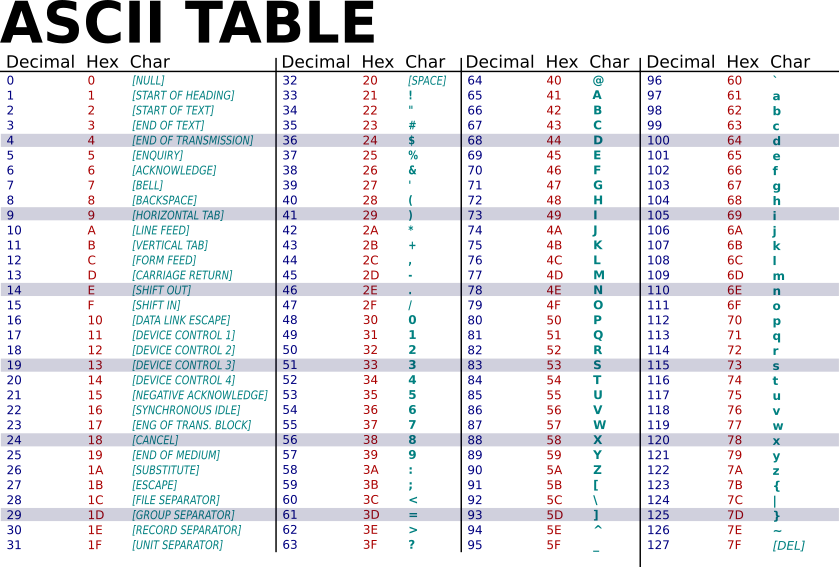
\includegraphics[width=\linewidth]{./gfx/ASCII_table}\newline
\caption
	[ASCII-Codes]
	{ASCII: American Standard Code for Information Interchange\newline
         Quelle: \url{source: https://commons.wikimedia.org/wiki/File:ASCII-Table-wide.svg}
    }
\label{fig:ASCII}
\end{figure}
Texte werden intern als Folge von Dezimalzahlen behandelt. Jedem Zeichen wird eine Zahl zugeordnet und mittels einer Tabelle \enquote{übersetzt}. Aus technischen Gründen ist die Zahl der darstellbaren Zeichen für einfache Programme auf 256 begrenzt\footnote{In der Vorlesung \emph{Algorithmen und Datenstrukturen} an der Universtität Regensburg können Sie erfahren, wie sie diese Schranke umgehen und so \eg internationale Schriftzeichen in ihren Programmierprojekten verwerten. Sie können sich hierzu auch selbst Wissen zum Stichword \emph{Unicode} aneignen.}. Davon sind die ersten 128 Zuordnungen international genormt; die zweite Hälfte der Tabelle hängt von den Ländereinstellungen am jeweiligen Rechner ab. Siehe Abb.\,\ref{fig:ASCII} für die Zuordnung.

Damit können wir mit den Mitteln der Elektronik bereits beliebig große positive Ganzzahlen und Schriftzeichen darstellen\footnote{negative Zahlen und Dezimalbrüche werden in Abschnitt \ref{sec:Datawidth} behandelt}. Wie aber schafft man es, aus Zahlen komplexe Programme zu bauen?

\section{Von Zahlen zu Befehlen} \label{sec:assembly}
Die \emph{CPU} (Central Processing Unit) eines Computers ist ein elektronisches Bauteil, in dem eine gewisse Anzahl sehr einfacher Arbeitsschritte \enquote{mechanisch} im Chip umgesetzt sind. Solche Arbeitsschritte sind etwa \enquote{addiere zwei Zahlen} oder \enquote{lade einen Wert vom Speicher}. Diese Befehle kann man sich als \enquote{durchnummeriert} denken. Ist \texttt{17} beispielsweise die Nummer des Befehls \texttt{multipliziere}, so drückt die Zahlenkette \texttt{17 21 2} also den Auftrag \texttt{multipliziere die Zahlen 21 und 2 miteinander} aus. Genau aus solchen Zahlenketten besteht jedes Computerprogramm. Die Zahlen werden im \emph{Binärformat} gespeichert, also als Kette von 0en und 1en, die auch als Schriftzeichen interpretiert werden könnten. Öffnet man mit einem Textbearbeitungsprogramm eine ausführbare Datei, so zeigt dieses nur einen unverständlichen Zeichensalat an. Für einen Menschen wäre es beschwerlich, eine solche Datei zu lesen; theoretisch ist es aber möglich, mithilfe einer geeigneten Tabelle ausführbare Dateien zu \enquote{lesen}.

In den Pioniertagen der Computertechnik musste man tatsächlich die Zuordnung der Zahlen zu den Befehlen kennen, um ein Computerprogramm zu schreiben. Diese Arbeitsweise ist selbstverständlich sehr umständlich und fehleranfällig. Erste Abhilfe schuf hier die Programmiersprache \emph{Assembler}. Jedem CPU-Befehl wurde ein kurzer Text zugeordnet, der für Menschen leichter zu lesen und zu merken ist: Zeilen wie \texttt{mul 21 2} erlauben bereits bedeutend komfortableres Schreiben und Warten von Programmen.

Die Programmierung in Assembler ist immer noch sehr kleinschrittig und erlaubt es kaum, komplexe Projekte umzusetzen\footnote{Die erste Generation der Gameboy-Spielereihe \emph{Pokémon} wurde in Assembler programmiert. Obgleich dies eine beachtliche Leistung darstellt sind diese Spiele heute bekannt für die Vielzahl von in diesen enthaltenen \emph{Glitches} (Fehlern im Code, die unbeabsichtigte Effekte auslösen)}. Aus diesem Grund wurden \emph{Hochsprachen} wie C entwickelt, in denen komplette \enquote{Arbeitspakete} wie \enquote{Gib einen Text auf dem Bildschirm aus} in einem einzelnen Befehl zusammengefasst sind. Damit diese C-Befehle vom Computer verstanden werden, müssen diese natürlich erst wieder in Maschinensprache zurückübersetzt werden, also in eine Folge von Zahlen, die die CPU interpretieren kann. Diese Aufgabe benutzt ein sogenannter \emph{Compiler}, also ein spezielles Computerprogramm\footnote{Tatsächlich wird häufig erst von der Hochsprache in Assembler übersetzt. Der letzte Schritt -- die Übersetzung von Assembler-Code in Maschinensprache -- übernimmt ein \emph{Assembler}. In der Praxis sagt man aber einfach \enquote{kompilieren} zur Gesamtheit aller Übersetzungsschritte bis hin zur Maschinensprache.}.

Ein Vorteil von Hochsprachen ist, dass man mit ihnen eigene Befehle definieren und so noch komplexere Konstrukte schreiben kann. Häufig wiederkehrende Aufgaben werden in sogenannten \emph{Bibliotheken} oder \emph{Libraries} gesammelt und -- oft schon \emph{vorkompiliert} (also bereits in Maschinensprache  übersetzt) -- anderen Programmierern zur Verfügung gestellt. So existiert in C beispielsweise die  \emph{math-library}, in der Operationen wie \emph{finde die Quadratwurzel einer Zahl} umgesetzt werden. Ein sogenannter \emph{Linker} sorgt dafür, dass Code aus eigenen Projekten und vordefinierten Libraries korrekt verknüpft werden.

\section{Aufruf des Compilers} \label{sec:Compile}
Für diesen Kurs benutzen wir den \emph{GNU C-Compiler} (gcc). Dieses Programm ist sowohl ein Compiler als auch ein Linker. Gehen wir davon aus, im aktuellen Arbeitsverzeichnis liegt eine Datei mit dem Namen \texttt{myCode.c} vor. Diese Datei kann kompiliert werden mit dem Kommandozeilen-Befehl:
\begin{cmdbox}[Kommandozeilen-Befehl: Kompilieren]
gcc myCode.c
\end{cmdbox}

Der gcc kompiliert mit diesem Befehl die Datei \texttt{myCode.c} und erstellt eine ausführbare Datei mit dem Dateinamen \texttt{a.out}. Diese kann nun über den Kommandozeilen-Befehl:
\begin{cmdbox}[Kommandozeilen-Befehl: Kompiliertes Programm ausführen]
./a.out
\end{cmdbox}
ausgeführt werden. Besteht der Code aus mehreren \emph{Modulen}\footnote{\ie mehrere Dateien; im Detail steckt mehr hinter diesem Begriff, worauf wir in Kapitel \ref{chp:modules} näher eingehen werden.}, so können diese einfach beim Aufruf des gcc hintereinander durch Leerzeichen getrennt aufgelistet werden. Neben Code-Dateien (Erweiterung \texttt{.c}) können auch vorkompilierte \enquote{Object Codes} (Erweiterung \texttt{.o}) aufgelistet werden.
\begin{cmdbox}[Kommandozeilen-Befehl: Kompilieren mehrerer Module]
gcc myCode.c otherCode.c moreCode.c objectFile.o otherObject.o
\end{cmdbox}

In jedem Fall wird die Datei \texttt{a.out} erstellt (bzw. überschrieben, falls diese schon existiert). Möchte man, dass das kompilierte Programm einen anderen Namen erhält, so kann die Option \texttt{-o [OutputName]} angegeben werden; \texttt{[OutputName]} ist dabei der neue Dateiname. Beispiel: die zu erstellende ausführbare Datei soll den Namen \texttt{myProgram} tragen:
\begin{cmdbox}[Kompilieren mit vorgegebenem Dateinamen für das kompilierte Programm]
gcc -o myProgram myCode.c
\end{cmdbox}
Entsprechend startet man dieses Programm dann mit der Zeile
\begin{cmdbox}[Kommandozeilen-Befehl: Kompiliertes Programm ausführen]
./myProgram
\end{cmdbox}

Während der Entwicklung eines Programmes wird man häufig Fehler machen. Manche dieser Fehler sorgen für Code, der vom Compiler nicht interpretiert werden kann; man spricht \ua von \emph{Syntaxfehlern}. Dies können beispielsweise fehlende Klammern sein. Enthält der Code solche Fehler, wird das Kompilieren abgebrochen und keine ausführbare Datei erzeugt. Stattdessen zeigt der Compiler Informationen zum Fehler in der Kommandozeile an. (Wir gehen in den folgenden Kapiteln genauer auf diese Rückmeldungen ein).

Andere Code-Elemente können zwar in \enquote{validen Maschinencode} umgesetzt werden, weisen aber auf logische Fehler hin. Standardmäßig gibt der Compiler hierzu keine Rückmeldung. Wir können aber mit den Kommandozeilenoptionen \texttt{-Wall}, \texttt{-Wimplicit-fallthrough} und \texttt{-Wpedantic} einstellen, dass auf solche Strukturen in der Compiler-Ausgabe ebenfalls hingewiesen werden soll. In der Compiler-Ausgabe werden diese dann als \emph{warnings} vermerkt (daher das \texttt{W} in \texttt{Wall}, \texttt{-Wimplicit-fallthrough} und \texttt{Wpedantic}). Ich empfehle sehr stark, diese Optionen zu nutzen und den Code so zu verbessern, bis alle Warnungen beseitigt sind; in meinen Projekten hat diese Funktion einige Fehler aufgedeckt und mir viel Zeit erspart.

Ein Aufruf mit diesen Optionen sieht also so aus:
\begin{cmdbox}[Kompilieren mit Ausgabe aller Warnungen]
gcc -Wall -Wimplicit-fallthrough -Wpedantic -o myProgram myCode.c
\end{cmdbox}

Bibliotheken (\eg \texttt{.o}-Dateien) liegen in der Regel nicht im aktuellen Arbeitsverzeichnis, sondern in einem Standard-Verzeichnis, so dass alle Codes auf der Festplatte diese gleichermaßen Nutzen können. Um dem Compiler mitzuteilen, dass eine solche Bibliothek mit in den Linking-Prozess einbezogen werden soll, benutzen wir die Kommandozeilen-Option \texttt{-l[library]}, wobei \texttt{[library]} der Name der Bibliothek ist, die einbezogen werden soll. Im Kurs wollen wir \eg desöfteren mathematische Funktionen aus der Mathe-Bibliothek \texttt{m} benutzen. entsprechend ergänzen wir den Compiler-Aufruf um die Option \texttt{-lm}:
\begin{cmdbox}[Kompilieren und Linken mit der math-library]
gcc -Wall -Wimplicit-fallthrough -Wpedantic -o myProgram -lm myCode.c
\end{cmdbox}

Im Vorwort wurde erwähnt, dass C laufend fortentwickelt wird. Dies hat Auswirkungen auf die Interpretation des Codes; derselbe Code wird von älteren Versionen des Compilers nicht zwangsweise in derselben Art umgesetzt wie von neueren. Der gcc kann sowohl nach älteren als auch neueren Versionen der Sprache C kompilieren. Welche Version der Sprache benutzt werden soll, wird mit der Kommandozeilenoption \texttt{-std=[standard]} angegeben. Im Kurs halten wir uns an den Standard aus dem Jahr 2011, und ergänzen den Kommandozeilen-Aufruf entsprechend um \texttt{-std=c11}:
\begin{cmdbox}[Kompilieren mit nach Standard C11]
gcc -std=c11 -Wall -Wimplicit-fallthrough -Wpedantic -o myProgram myCode.c -lm
\end{cmdbox}

Neben den gezeigten Optionen existieren noch viele weitere Schalter, über die die Arbeitsweise des Compilers beeinflusst werden können; auf diese soll hier jedoch nicht weiter eingegangen werden. Interessierte KursteilnehmerInnen können mit dem Befehl \texttt{man} eine Übersicht aller Optionen mit Erklärungen anzeigen lassen.
\begin{cmdbox}[man-page des gcc]
man gcc
\end{cmdbox}

\begin{plusbox}
Die hier gegebenen Erklärungen und Optionen gelten so auch für C++. Jedoch sollte der Compiler \texttt{g++} benutzt werden. Das heißt, an allen Stellen, in denen oben \texttt{gcc} stand, muss durch \texttt{g++} ersetzt werden. Außerdem muss Als Standard muss dann \texttt{-std=c++11} angegeben werden.
\end{plusbox}

\begin{hintbox}
Da es lästig werden kann, wiederholt dieselben Optionen zu tippen, arbeite ich für kleinere Projekte gerne mit einem kleinen Script wie dem folgenden\footnote{Für größere Projekte gibt es Mechaniken, die hier nicht angesprochen werden können. Interessierte KursteilnehmerInnen können die DozentInnen bei Interesse auf \emph{makefiles} ansprechen.}:
\begin{codebox}[Mini-Script \texttt{compile} zum komfortablen kompilieren]
\begin{minted}[linenos]{bash}
OPTIONS="-std=c11 -Wall -Wimplicit-fallthrough -Wpedantic"
LIBS="-lm -lncurses"

INFILE=$1
OUTFILE="${INFILE%%.*}"

clear

rm -f $OUTFILE
echo ==================================
echo attempting to compile
echo gcc $OPTIONS -o $OUTFILE $INFILE $LIBS 
echo ..................................
echo ""

gcc $OPTIONS -o $OUTFILE $INFILE $LIBS 

echo ""
echo ..................................
echo Compilation successfull.
echo ..................................
echo ""
./$OUTFILE
\end{minted}
\end{codebox}

Dieses Script kann \eg in einer Textdatei mit Namen \texttt{compile} gespeichert und als ausführbares Script markiert werden. Letzeres geschieht über einen Kommandozeilen-Befehl:
\begin{cmdbox}[Kommandozeile: Script ausführbar machen]
chmod +x ./compile
\end{cmdbox}

Mit diesen Schritten reicht es, nur noch
\begin{cmdbox}[Kommandozeile: Script ausführen]
./compile myCode.c
\end{cmdbox}
einzugeben. Der Code automatisch mit den besprochenen Optionen kompiliert und direkt ausgeführt, sofern der Code erfolgreich kompiliert werden konnte.
\end{hintbox}
	\chapter{Ein erstes Programm}
\epigraph{The secret to getting ahead is getting started.}{Mark Twain}
In diesem Kapitel werden wir zunächst ein sogenanntes \emph{Hello World} besprechen: Dieses Programm gibt einen kurzen Text auf dem Bildschirm aus und enthält sonst \enquote{nur} den Grundaufbau eines C-Programms\footnote{Der Begriff \emph{Hello World} wird auch im Kontext anderer Sprachen benutzt und bedeutet dort dasselbe.}. Im Weiteren betrachten wir auch Möglichkeiten, die Sprache C für einfache Rechnungen zu verwenden.

\section{Hello World}
Die folgenden Zeilen zeigen ein Programm, das den Text \texttt{Hello World!} auf dem Bildschirm ausgibt.
\begin{codebox}
\begin{minted}[linenos]{c}
#include <stdio.h>

int main() {
   printf("Hello World!\n");
}
\end{minted}
\end{codebox}
Betrachten wir den Code Zeile für Zeile.

Es wurde bereits angesprochen, dass häufig wiederkehrende Aufgaben in Bibliotheken ausgelagert werden können und so in vielen Projekten zur Verfügung stehen. Eine solche Bibliothek stellt Routinen zur Ein-und Ausgabe bereit und trägt den Namen \texttt{stdio} (\emph{standard in/output}). Um die Routinen im Code nutzbar zu machen, müssen diese einmalig \emph{deklariert} werden. Mit dem Befehl \mintinline{c}{#include} wird die Datei \texttt{stdio.h} in den Code mit eingebunden\footnote{Die Datei befindet sich in einem Standard-Verzeichnis, das bei der Installlation des gcc angelegt und voreingestellt wird.}. Diese Datei wird ein \emph{Header} genannt und enthält alle notwendigen Deklarationen für die Textein- und Ausgabe. In Kapitel \ref{chp:modules} werden wir hierauf zurück kommen. Für den Moment reicht es zu wissen, dass die \mintinline{c}{#include}-Zeile notwendig ist, um Ein/Ausgabe-Befehle benutzen zu können.

Programme sind in funktionelle Einheiten (\enquote{Funktionen}) gegliedert, die von \{geschweiften Klammern\} eingefasst werden. Zeile 3 deklariert eine solche Funktion mit Namen \texttt{main}, die bis Zeile 5 reicht. Ein Programm kann beliebig viele solcher Funktionen besitzen, die sich jeweils im Namen unterscheiden müssen. Groß- und Kleinschreibung wird beachtet, \texttt{main} ist also von \texttt{Main} verschieden. Die Funktion \texttt{main} ist das Hauptprogramm; nur dieses wird automatisch ausgeführt. Auch hierzu werden wir in Kapitel \ref{chp:funcs} vertiefen (insbeseondere die Bedeutung von \mintinline{c}{int} und den Klammern). Für unsere ersten Programme können wir diese Zeile einfach kopieren.

Zeile 4 enthält den Befehl \texttt{printf}. Dieser Befehl gibt Text auf dem Bildschirm aus. (Das \texttt{f} in \texttt{printf} steht dabei für \emph{formatted}. In Abschnitt \ref{sec:formattedOutput} werden wir einige Details hierzu kennen lernen.) Welcher Text das ist, wird als \emph{Parameter} übergeben, \ie in Klammern hinter den Befehl selbst gestellt. Hier also ist der Parameter zu \texttt{printf} der Ausdruck \texttt{"Hello World!\textbackslash n"}. Um Texte von restlichem Code abzugrenzen muss der Text in \texttt{"}doppelte Anführungszeichen\texttt{"} gesetzt werden. Dieser Text enthält auch einen Zeilenumbruch, codiert als \texttt{\textbackslash n} (n für \emph{new line}).

Wichtig ist das Semikolon (;) am Ende der Zeile -- hiermit wird ein Befehl abgeschlossen. Jeder Befehl muss mit einem Semikolon abgeschlossen werden. Fehlt dieses, gibt der Compiler eine Fehlermeldung aus und bricht die Kompilation ab. Mehrere Befehle dürfen in derselben Zeile stehen, solange diese von einem Semikolon voneinander abgetrennt sind.

Wir können beliebig Leerzeichen, Tabulatoren oder Zeilenumbrüche in den Code einfügen, um diesem eine optische Struktur zu geben. Nur die \emph{Schlüsselwörter} (\eg Befehle, bzw. die \enquote{Worte} des Codes) dürfen nicht zertrennt werden. Einrückungen werden verwendet, um \enquote{Hierarchieebenen} zu verdeutlichen und machen den Code besser les- und wartbar. Ich empfehle, gleich von Anfang an Einrückungen wie in diesem Script gezeigt zu verwenden. Vom Compiler werden Leerzeilen komplett ignoriert und können zur Abgrenzung von Codeblöcken beliebig eingefügt werden.

Der folgende Code erzeugt dasselbe Ergebnis wie oben und soll nur verdeutlichen, wo Leerzeichen eingefügt werden können.
\begin{codebox}
\begin{minted}[linenos]{c}
  #include     <stdio.h>
  int    main   (   )    {
      printf   (   "Hello World!\n"   )   ;
   }
\end{minted}
\end{codebox}

Code wird vom Compiler von oben nach unten gelesen und bearbeitet. Die Reihenfolge der einzelnen Anweisungen ist also von großer Bedeutung. Verschiebt man beispielsweise die \mintinline{c}{#include}-Zeile an das Ende des Codes, so erhält man Fehlermeldungen, da der Befehl \texttt{printf} deklariert werden muss (durch Einbinden der Datei \texttt{stdio.h}) \emph{bevor} er zum ersten Mal aufgerufen wird.

\section{Variablen, Datentypen, Operatoren} \label{sec:expressions}
Nützliche Programme entwickeln sich über die Zeit, berechnen also \eg ein Ergebnis oder reagieren auf Benutzereingaben. Um dies zu ermöglichen, existieren in C \emph{Variablen}, also Symbole, die einen Wert beschreiben, der sich über die \emph{Laufzeit} eines Programmes ändern.

\subsection{Variablen}
Eine Variable hat einen Namen, einen \emph{Datentyp} und einen Wert.

Der Name einer Variablen ist eine beliebige Kombination aus \emph{alphanumerischen Zeichen}\footnote{Die Buchstaben a-z, A-Z, die Ziffern 0-9 sowie der Unterstrich (\_), jedoch keine Umlaute, Sonderzeichen oder das scharfe ß.}. Er muss mit einem Buchstaben beginnen, darf keine Leerzeichen enthalten und kann bis zu 40 Zeichen lang sein. Auch hier wird zwischen Groß- und Kleinschreibung unterschieden. Variablennamen müssen \emph{eindeutig} sein, \ie es darf keine zwei Variablen mit demselben Namen geben. Auch Funktionsnamen gelten als \enquote{verbraucht}; wir können keine Variable \texttt{main} nennen.

Anfänger neigen dazu, sehr kurze, nichtssagende Variablennamen zu vergeben. Um Programme gut les- und wartbar zu machen (und um somit Fehler zu vermeiden) sollte der Variablenname bereits ihre Funktion im Code angeben. Statt \texttt{a, b, c} also lieber \texttt{elementCount, averageNote, currentIndex}.

Unter \emph{Datentyp} versteht man die Art der Information, die in der Variablen gespeichert wird, \eg Ganzzahl, Kommazahl oder Text. Dies ist notwendig, da der Computer intern nur Einsen und Nullen speichern kann. Ohne Kontext ist es also nicht möglich, zu erkennen, wie eine Bit-Folge zu interpretieren ist. Dieser Kontext ist durch Zuweisung eines Datentyps gegeben.

Der Wert einer Variablen kann schließlich alles sein, was ihrem Datentypen entspricht; eine Variable kann \eg eine einzelne Zahl oder ein ganzes Bild speichern.

\subsection{Variablen Deklarieren} \label{sec:DeclareVars}
Um Variablen zu benutzen müssen diese zuerst \emph{deklariert} werden. Dies geschieht in der Form
\begin{codebox}[Syntax: Variablen Deklarieren]
\texttt{Datentyp VariablenName;}
\end{codebox}
Mehrere Variablen können in einem Schritt deklariert werden, indem man sie durch Kommata voneinander abtrennt.

Für den Moment wollen wir uns auf die Datentypen \mintinline{c}{int} (Ganzzahlen) und \mintinline{c}{double} (Kommazahlen) beschränken. Mit diesen können wir also folgende Variablen deklarieren:
\begin{codebox}[Beispiel: Deklaration von mehreren Variablen]
\begin{minted}[linenos]{c}
int main () {
   int    Ganzzahl;
   double Kommazahl, andereZahl;
}
\end{minted}
\end{codebox}
Variablen werden also \emph{innerhalb von Funktionen} deklariert\footnote{In Abschnitt \ref{sec:globals} werden wir hierzu mehr hören; für den Moment beschränken wir uns auf den Fall, dass alle Variablen am Anfang der Funktion \texttt{main} deklariert werden.}.

Ihnen mag die Ähnlichkeit zwischen der Deklaration von Ganzzahl-Variablen und der Funktion \texttt{main} aufgefallen sein. Dies ist kein Zufall. Tatsächlich ist formell die Funktion \texttt{main} die Vorschrift einen \mintinline{c}{int}-Wert zu berechnen. Das Symbol \texttt{main} ist eine Variable, die auf diese Vorschrift verweist. Hierzu mehr in Kapitel \ref{chp:OS-Link}.

\subsection{Wertezuweisung} \label{sec:valueAssignment}
Werte können über den \emph{Operator} = zugewiesen werden:
\begin{codebox}[Beispiel: Wertzuweisung]
\begin{minted}[linenos]{c}
int main () {
  int    Ganzzahl;
  double Kommazahl, andereZahl;
  
  Ganzzahl   = 7;
  Ganzzahl   = 8;
\end{minted}
\end{codebox}

\begin{codebox}[]
\begin{minted}[linenos, firstnumber=last]{c}
   Kommazahl  = 4.3;
   andereZahl = 5.0;
}
\end{minted}
\end{codebox}

In Zeile 5 wird also der Variablen \texttt{Ganzzahl} der Wert 7 zugewiesen. In der folgenden Zeile 6 überschreiben wir diesen Wert mit dem Wert 8.

In den Zeilen 7 und 8 erhalten die beiden \mintinline{c}{double}-Variablen ebenfalls Werte. Wir bemerken, dass hier ein \emph{Dezimalpunkt} gesetzt wird, also kein Komma.

Deklaration und Wertzuweisung können auch in einem einzigen Schritt geschehen:
\begin{codebox}[Beispiel: Kombinierte Deklaration und Wertzuweisung]
\begin{minted}[linenos]{c}
int main () {
   int    Ganzzahl   = 8;
   double Kommazahl  = 4.3,
          andereZahl = 5.0;
}
\end{minted}
\end{codebox}

\begin{hintbox}[Nicht-Initialisierte Variablen]
Wenn eine Variable deklariert wird, sorgt der Compiler lediglich dafür, dass genug Platz im Speicher reserviert wird, um diesen Wert zu erfassen. Im Allgemeinen wird aber kein bestimmter \enquote{Startwert} festgelegt. Die neue Variable startet mit dem Wert, den das Bitmuster an der Stelle festlegt, an der Platz für die Variable reserviert wurde. Dies ist ein zufälliger Wert! Programme, die mit einem solchen Zufallswert weiterarbeiten haben generell \emph{undefiniertes} Verhalten und können abstürzen oder sogar Schaden anrichten. Es ist daher also ratsam, allen Variablen bei der Deklaration gleich einen sinnvollen oder sicheren Startwert zuzuweisen.
\end{hintbox}

\begin{hintbox}[Fließkommazahlen ohne Nachkommastelle]
In der Mathematik gilt $5 = 5.0$. Ein Computer arbeitet zwar nach mathematischen Prinzipien; streng genommen gilt diese Gleichheit für den Prozessor aber nicht. Wie wir in Abschnitt \ref{sec:DataRepresentation} sehen werden kann dieselbe (mathematische) Zahl auf verschiedene Weisen binär dargestellt werden. Insbesondere zwischen Ganzzahlen und Kommazahlen bestehen große Unterschiede in der Binär-Darstellung. Der gcc kann zwar Umwandlungen automatisch durchführen, und würde auch
\begin{codebox}[Beispiel: Implizite Typumwandlung von Ganzzahl zu Fließkommazahl]
\begin{minted}[linenos]{c}
int main () {
   double Kommazahl = 5;
}
\end{minted}
\end{codebox}
\enquote{korrekt} umsetzen. Hier wird versucht, die \emph{Ganzzahl} \texttt{5} in der \mintinline{c}{double}-Variablen \texttt{Kommazahl} zu speichern. Da dies direkt nicht möglich ist, wandelt der gcc diese Ganzzahl zuerst in die Fließkommazahl \texttt{5.0} um und speichert dann diese. Eine solche \emph{implizite Typumwandlung} kann aber unbeabsichtigte Nebeneffekte haben und sollte daher vermieden werden. Als Beispiel für solche Nebeneffekte möchte ich Ihnen das folgende Beispiel geben:
\end{hintbox}
%
\begin{hintbox}[]
\begin{codebox}[Beispiel: Implizite Typumwandlung von Fließkommazahl zu Ganzzahl]
\begin{minted}[linenos]{c}
int main () {
   int Ganzzahl = 5.5;
}
\end{minted}
\end{codebox}
Analog zum Beispiel oben wird nun implizit die Zahl \texttt{5.5} zu einer Ganzzahl konvertiert. Natürlich ist Ihnen bewusst, dass es keine ganze Zahl gibt, die gleich $5.5$ ist. Es wird also gerundet. Im Gegensatz zur menschlichen Intuition rundet der gcc hier aber \emph{ab}. Außerdem können die \enquote{fehlenden} $0.5$ das Verhalten des Programms in der Laufzeit gegenüber der Erwartung verändern.

Damit der Datentyp (und damit das Verhalten des Programms) immer ersichtlich ist, sollten daher \enquote{ganzzahlige Fließkommawerte} als Kommawert (\eg \texttt{5.0}) gesetzt werden.
\end{hintbox}

\subsection{Rechnen mit Variablen -- Operatoren}\label{sec:OperatorsArithmetic}
Mit Variablen kann auch gerechnet werden. Hierzu stehen 6 \enquote{Grundrechenarten} zur Verfügung (siehe Tabelle \ref{tab:OperatorsArithmetic}). Mehrere solche Rechenoperationen können hintereinander geschaltet werden. Es gilt wie üblich Punkt-vor-Strich; Klammern können gesetzt werden um eine andere Reihenfolge festzulegen.
\begin{table}[h!]
	\newcolumntype{C}{>{\ttfamily\centering\arraybackslash} p{.2\linewidth}}
\begin{center}
\begin{tabularx}
	{.95\linewidth}
	{cC|cC}
\toprule[1pt]
	
	Operation   & \normalfont Zeichen  &  Operation                              & \normalfont Zeichen
\tabcrlf
	Addition    & +                    &  Multiplikation                         & * \\
	Subtraktion & -                    &  Division                               & / \\
	Negation    & -                    &  Rest der Division (\enquote{Modulo})   & \%\\
	
\bottomrule[1pt]
\end{tabularx}
\end{center}
\caption{Rechenoperatoren in C}\label{tab:OperatorsArithmetic}
\end{table}

\begin{codebox}[Beispiel: Rechnen mit Variablen]
\begin{minted}[linenos]{c}
int main () {
   int    Ganzzahl;
   double Kommazahl, andereZahl;
   
   Ganzzahl   = 7;
   Ganzzahl   = Ganzzahl + 8;
   
   Kommazahl  = 4.3;
   andereZahl = 3.0 * (-Kommazahl + 7.9) / 2.0;
}
\end{minted}
\end{codebox}

Wichtig ist, dass Variablen bereits deklariert sind \emph{bevor} auf sie verwiesen wird, \ie bevor sie in anderen Ausdrücken vorkommen. Folgendes Beispiel funktioniert daher nicht:
\begin{codebox}[Beispiel: Fehlerhafter Code{,} Variablen zu spät deklariert]
\begin{minted}[linenos]{c}
int main () {
  Ganzzahl = 7;
  int Ganzzahl;
}
\end{minted}
\end{codebox}
und erzeugt die folgende Fehlermeldung:
\begin{cmdbox}[Fehlermeldungen des gcc]
\begin{minted}{text}
myProgram.c: In function ‘main’:
myProgram.c:2:4: error: ‘Ganzzahl’ undeclared (first use in this 
function)
    Ganzzahl = 7;
    ^~~~~~~~
myProgram.c:2:4: note: each undeclared identifier is reported only once 
for each function it appears in
\end{minted}
\end{cmdbox}
Jede Fehlermeldung beginnt mit einem Verweis auf die Fehlerhafte Datei und die Funktion darin, in der das Problem aufgetreten ist (\texttt{myProgram.c: In function ‘main’:}). In der folgenden Zeile der Fehlerausgabe wird genauer spezifiziert in welcher Zeile, und an welcher Stelle der Fehler auftrat (\texttt{myProgram.c:2:4}, also  Zeile 2, Spalte 4) und welcher Fehler gefunden wurde (\texttt{‘Ganzzahl’ undeclared}). Schließlich gibt der Compiler noch die relevante Stelle aus und markiert die kritische Stelle.

\begin{hintbox}[Zur Division mit Ganzzahl- und Fließkomma-Werten]
Der Datentyp einer Division hängt vom Datentyp von Divisor und Dividend ab. Ist einer der beiden ein Fließkommawert, so wird auch das Ergebnis als Fließkommawert berechnet. Sind beide Werte Ganzzahlen, wird auch das Ergebnis als Ganzzahl berechnet und gegebenenfalls abgerundet. Betrachten wir folgendes Beispiel:
\begin{codebox}[Beispiel: Division von Ganzzahlen und Fließkommazahlen]
\begin{minted}[linenos]{c}
double x = 3   / 2  ,
       y = 3.0 / 2.0,
       z = 3.0 / 2  ,
       w = 3   / 2.0;
\end{minted}
\end{codebox}
Die Variable \texttt{x} geht aus der Division zweier Ganzzahlen hervor, und wird damit zu \texttt{1.0} abgerundet. Bei der Berechnung von \texttt{y} hingegen gehen Fließkommazahlen in die Division ein; somit wird das Ergebnis nicht gerundet und als 1.5 gespeichert. Dasselbe gilt für \texttt{z} und \texttt{w}, da zumindest \emph{eine} der an der Division beteiligten Zahlen eine Fließkommazahl war.
\end{hintbox}

\subsection{Shorthands}
Häufig soll sich der Wert einer Variablen \emph{inkrementiert} (\enquote{hochgezählt}) werden. Dies kann codiert werden als:
\begin{codebox}[Beispiel: Inkrementieren einer Variablen i]
\begin{minted}[linenos]{c}
int main () {
   int i = 5;
   i = i + 1;  // i hat jetzt den Wert 6
}
\end{minted}
\end{codebox}

Daneben gibt es auch den \emph{Shorthand} (Kurzform) \texttt{variable++}:
\begin{codebox}[Beispiel: Inkrementieren einer Variablen i mit Shorthand ++]
\begin{minted}[linenos]{c}
int main () {
   int i = 5;
   i++;       // i hat jetzt den Wert 6
}
\end{minted}
\end{codebox}

In beiden Beispielen wird der Wert von \texttt{i} in Zeile 3 um 1 erhöht.

Analog dazu existiert der \emph{Dekrement}-Operator \texttt{variable-{}-}, der den Wert von \texttt{variable} um 1 verringert.

Weiter existieren der Operator-Shorthand \texttt{variable += expression}. Zu \texttt{variable} wird der Wert von \texttt{expression} hinzugezählt und anschließend in \texttt{variable} gespeichert. \texttt{expresion} darf dabei ein beliebig komplexer Ausdruck sein:
\begin{codebox}[Beispiel: Inkrementieren einer Variablen i mit Shorthand \texttt{+=}]
\begin{minted}[linenos]{c}
int main () {
   int i = 5,
       j = 2;
   i += 3 * j + 1;
}
\end{minted}
\end{codebox}
Hier wird zunächst der Ausdruck \texttt{3 * j + 1} ausgewertet zu \texttt{7}; als nächster Schritt wird die Summe \texttt{i + 7} berechnet, und diese dann in \texttt{i} gespeichert. Die Variable \texttt{i} hat also nach Zeile 4 den Wert 12.

Analog existieren auch die Shorthands \texttt{-=}, \texttt{*=}, \texttt{/=} und \texttt{\%=}. 

\begin{hintbox}[Inkrement und Dekrement: Prefix und Postfix]
Die Operatoren \texttt{++} und \texttt{-{}-} können sowohl \emph{vor} als auch \texttt{hinter} einen Ausdruck gesetzt werden (Wir sprechen von \emph{Prefix} und \emph{Postfix}). Für sich alleine ist in beiden Fällen der Effekt derselbe -- der Wert des Ausdrucks wird um 1 erhöht bzw. Verringert. Kombiniert mit anderen Operationen ergeben sich aber Unterschiede. Betrachten wir folgendes Beispiel:

\begin{codebox}[Beispiel: Unterschiede bei Prefix- und Postfix-Inkrement]
\begin{minted}[linenos]{c}
int main () {
   int i, j;
   
   // Postfix-Form
   i = 5;
   j = i++;		// i = 6, j = 5.
   
   // Prefix-Form
   i = 5;
   j = ++i;		// i = 6, j = 6.
}
\end{minted}
\end{codebox}

In der Postfix-Form (Zeile 6) wird zuerst der Wert von \texttt{i} gelesen und der Variablen \texttt{j} zugewiesen; danach wird \texttt{i} inkrementiert.

Bei der Prefix-Form (Zeile 10) dagegen wird zuerst \texttt{i} inkrementiert und danach der Wert von \texttt{i} in \texttt{j} gespeichert.
\end{hintbox}
%
\begin{hintbox}[]
Um den Code leicht les- und wartbar zu halten, empfehle ich, alle gedanklichen Schritte in abgeschlossene Befehle zu setzen. Äquivalent zum obigen Code ist der folgende, intuitiv leichter verständliche Code:

\begin{codebox}[Beispiel: Äquivalente Codes]
\begin{minted}[linenos]{c}
int main () {
   int i, j;
   
   // zur Postfix-Form
   i = 5;
   j = i;
   i++;		// i = 6, j = 5.
   
   // zur Prefix-Form
   i = 5;
   i++;
   j = i;		// i = 6, j = 6.
}
\end{minted}
\end{codebox}
\end{hintbox}

\section{Formatierte Ausgabe}\label{sec:formattedOutput}
Wir wollen nun auch die berechneten Ergebnisse in Erfahrung bringen. Dazu können wir den bereits bekannten Befehl \texttt{printf} benutzen. Betrachten wir folgendes Beispiel:

\begin{codebox}[Beispiel: Ausgabe einer Berechnung mit \texttt{printf}]
\begin{minted}[linenos]{c}
#include <stdio.h>

int main () {
   double result = 5.0 / 7.0;
   
   printf("5.0 / 7.0 = %lf\n", result);
}
\end{minted}
\end{codebox}

Die Ausgabe lautet:
\begin{cmdbox}[Ausgabe einer Berechnung mit \texttt{printf}]
5.0 / 7.0 = 0.714286
\end{cmdbox}

Wie oben besprochen wird zuerst in Zeile 4 das Ergebnis der Division zweier Fließkommazahlen berechnet und in der Variablen \texttt{result} gespeichert. Zur Ausgabe auf dem Bildschirm übergeben wir dem Befehl \texttt{printf} jetzt \emph{zwei} Argumente:

Das erste Argument wird \emph{Format-String} genannt und ist in unserem Beispiel der Anteil:
\begin{center}
\mintinline{c}{"5.0 / 7.0 = %lf\n"}.
\end{center}

Ein Format-String ist eine Zeichenkette, die besondere \emph{Platzhalter} enthält. Diese beginnen mit dem Zeichen \texttt{\%} gefolgt von einem oder mehreren Zeichen, die beschreiben, wofür Platz freigehalten werden soll. In diesem Fall steht der Platzhalter \texttt{\%lf}, was für eine \mintinline{c}{double}-Zahl steht. Diese Zahl wird hinter dem Format-String genannt und von diesem durch ein Komma abgetrennt. Andere Platzhalter-Symbole sind in Tabelle \ref{tab:FormatOutNum} aufgelistet.

In einem Format-String können beliebig viele Platzhalter stehen; für jeden Platzhalter muss eine entsprechende Einsetzung hinter dem Formatstring selbst genannt werden. 
\begin{codebox}[Beispiel: Ausgabe mehrerer Werte mit \texttt{printf}]
\begin{minted}[linenos]{c}
#include <stdio.h>

int main () {
   double f = 3.14;
   int    g = 42;
   
   printf(
      "Ganzzahl i = %d, Fliesskommazahl d = %lf, weitere Zahl = %d",
                    g,                      f,                  99);
}
\end{minted}
\end{codebox}

Werden hinter dem Formatstring zu viele oder zu wenige Werte angegeben, so meldet der Compiler eine Warnung:
\begin{cmdbox}[Warnung bei zu wenigen Argumenten für den Formatstring]
\begin{minted}{text}
myProgram.c: In function ‘main’:
myProgram.c:4:12: warning: format ‘%i’ expects a matching ‘int’ argument 
[-Wformat=]
   printf("%i\n");
           ~^
\end{minted}
\end{cmdbox}
Das Programm wird jedoch \enquote{erfolgreich} kompiliert und ausgeführt. An Stelle des Platzhalters wird ein zufälliger Wert vom Speicher eingesetzt\footnote{Bugs dieser Art sind leider häufig. Der im Jahr 2014 entdeckte \emph{Heartbleed-Bug} in der OpenSSL-Library geht auf einen ähnlichen Mechanismus zurück. Hacker konnten \enquote{fehlerhafte Anfragen} an einen Server schicken und so den Speicherinhalt des Servers auslesen -- und damit \eg Zugangsdaten der User auslesen. Compiler-Warnungen sollten also sehr ernst genommen werden.}.

Ähnliches stellen wir fest, wenn wir das folgende Beispiel betrachten:

\begin{codebox}[Beispiel: Ausgabe mehrerer Werte mit \texttt{printf}]
\begin{minted}[linenos]{c}
#include <stdio.h>

int main () {
   printf("%d\n", 1.5);
}
\end{minted}
\end{codebox}
Der Formatstring \texttt{\%d} beschreibt die Ausgabe einer \emph{Ganzzahl}; als Wert für diesen Platzhalter wird aber eine Fließkommazahl angeboten. Die Compiler-Warnung:

\begin{cmdbox}[Warnung bei falscher Zuordnung Platzhalter/Datensatz]
\begin{minted}{text}
myProgram.c: In function ‘main’:
myProgram.c:4:12: warning: format ‘%d’ expects argument of type ‘int’, but 
argument 2 has type ‘double’ [-Wformat=]
   printf("%d\n", 1.5);
           ~^
           %f
\end{minted}
\end{cmdbox}
weist darauf hin, dass die Ausgabe mit \texttt{\%d} für Fließkommawerte ungeeignet ist (und weist auf die Möglichkeit hin, mit \texttt{\%f} auszugeben). Trotz dieses Fehlers kann das Programm umgesetzt und erfolgreich ausgeführt werden. Angezeigt wird aber nicht \texttt{1.5}, sondern \texttt{-2102427368}. Diese Zahl ergibt sich, wenn das Bitmuster der Zahl \texttt{1.5} als Ganzzahl interpretiert wird\footnote{Genauer: Die ersten 32 bit des Bitmusters; \texttt{1.5} ist eine double-Zahl und damit 64 bit breit. In jedem Fall ist diese Ausgabe \enquote{unsinnig}.}.

Wir hatten zuvor schon \texttt{\textbackslash n} als Umschreibung des Zeilenumbruchs kennengelernt. Diese Umschreibung bestimmter Zeichen nennen wir \emph{Escape-Sequence}. Solche Escape-Sequenzen werden benutzt um Zeichen einzufügen, die Teil der C-Syntax sind und sonst nur schwer auf dem Bildschirm ausgegeben werden können. In diesem Kurs werden wir \texttt{\textbackslash n} (Zeilenumbruch), \texttt{\textbackslash \textbackslash} (Backslash) und \texttt{\textbackslash ''} (Anführungszeichen) häufiger sehen.

In den Tabellen \ref{tab:FormatOutNum} und \ref{tab:FormatOutSpc} im Anhang sind die wichtigsten Codes für Platzhalter und Escape-Sequenzen aufgelistet.

Formatstrings legen nicht nur den \emph{Datentyp} der Ausgabe fest. Zusätzlich kann eine Information hinterlegt werden, wie viel Platz auf dem Bildschirm benutzt werden soll. Auf diese Weise können tabellarische Ausgaben stattfinden. Zu diesem Zweck setzt man zwischen das \texttt{\%} und dem Platzhalter-Symbol (\eg \texttt{d} für Ganzzahl) eine Zahl:

\begin{codebox}[Beispiel: Format-String mit Platzangabe (1)]
\begin{minted}[linenos]{c}
#include <stdio.h>

int main () {
   printf("Text %3d\n", 1);
   printf("Text %3d\n", 10);
   printf("Text %3d\n", 100);
   printf("Text %3d\n", 1000);
}
\end{minted}
\end{codebox}

\begin{cmdbox}[Ausgabebeispiel: Format-String mit Platzangabe (1)]
\begin{minted}{text}
Text   1
Text  10
Text 100
Text 1000
\end{minted}
\end{cmdbox}

Sie sehen also dass die ersten drei Zeilen rechtsbündig ausgegeben. Dies liegt daran, dass mit \texttt{\%3d} drei Textzeichen für einen Ganzzahl-Wert vorgesehen werden. Die vierte Zeile enthält eine Zahl, die länger ist als die vorgesehenen drei Zeichen. Daher erfolgt die Ausgabe, als wäre keine Zahl eingefügt.

Es gibt auch die Möglichkeit, Platz linksbündig zu reservieren. In diesem Fall gibt man negative Zahlen an:


\begin{codebox}[Beispiel: Format-String mit Platzangabe (2)]
\begin{minted}[linenos]{c}
#include <stdio.h>

int main () {
   printf("Text %-3d Text\n", 1);
   printf("Text %-3d Text\n", 10);
   printf("Text %-3d Text\n", 100);
   printf("Text %-3d Text\n", 1000);
}
\end{minted}
\end{codebox}

\begin{cmdbox}[Ausgabebeispiel: Format-String mit Platzangabe (2)]
\begin{minted}{text}
Text 1   Text
Text 10  Text
Text 100 Text
Text 1000 Text
\end{minted}
\end{cmdbox}

Bei Fließkommazahlen können wir zusätzlich zum Gesamtplatz für die Ausgabe auch angeben, wie viele Stellen hinter dem Komma angegeben werden sollen. Die Ausgabe wird dabei automatisch gerundet, wenn weniger Nachkommastellen angegeben werden als die auszugebende Zahl:

\begin{codebox}[Beispiel: Format-String mit Platzangabe (3)]
\begin{minted}[linenos]{c}
#include <stdio.h>

int main () {
   printf("Text %5.3lf Text\n", 1.5);
   printf("Text %5.3lf Text\n", 1.555);
   printf("Text %5.3lf Text\n", 1.5555);
   printf("Text %5.3lf Text\n", 15.0);
}
\end{minted}
\end{codebox}

\begin{cmdbox}[Ausgabebeispiel: Format-String mit Platzangabe (3)]
\begin{minted}{text}
Text 1.500 Text
Text 1.555 Text
Text 1.556 Text
Text 15.000 Text
\end{minted}
\end{cmdbox}

\section{Kommentare}
Im Optimalfall ist Code selbsterklärend. \enquote{Sprechende} Variablennamen und gute Struktur erlauben, viele Zusammenhänge intuitiv zu erfassen. Dennoch ist es oft notwendig (und dann auch guter Stil), Programme mit Kommentaren zu versehen.

Kommentare können auf zwei Arten gesetzt werden:
\begin{itemize}
\item Mehrzeilige Kommentare beginnen mit \texttt{/*} und enden mit \texttt{*/}. Achtung: Kommentare können nicht \enquote{verschachtelt} werden!
\item Einzeilige Kommentare werden durch zwei \emph{forward slashes} \texttt{//} eingeleitet. Sie enden mit dem nächsten Zeilenumbruch\footnote{Diese Form der Kommentare ist erst seit dem Standard C99 aus dem Jahr 1999 zulässig; davor existierte nur die \enquote{Sternchen-Form}.}.
\end{itemize}

\begin{codebox}[Beispiel: Kommentare]
\begin{minted}[linenos]{c}
int main () {
   int i = 0;
   i++;  // Inkrement-Shorthand
   // Das ist noch ein einzilger Kommentar.

   /* Kommentar der sich über mehrere Zeilen erstreckt.
    * Oft setzt man weitere Sternchen an den Zeilenanfang, dies
    * dient aber nur optischen Zwecken und kann
      nach belieben ausgelassen werden.
    */
    
   /* "Stern-Form" auch für einzeilige Kommentare */
   
   /* Ein weiterer Kommentar
    *  /* FEHLER -- keine verschachtelten Kommentare */ 
    */
}
\end{minted}
\end{codebox}

\section{Hello World in C++}
\begin{plusbox}
Die hier gegebenen Erklärungen und Optionen gelten so auch für C++. Das bedeutet, dass der oben gezeigte Code auch in C++ so kompiliert werden kann und dasselbe Ergebnis erzeugt. Jedoch steht hier für die Textausgabe auch das Konzept \emph{Streams} zur Verfügung. Betrachten wir den folgenden Code:

\begin{codebox}[Beispiel: Hello World in C++]
\begin{minted}[linenos]{c++}
#include <iostream>

int main() {
   std::cout << "Hello world!" << std::endl;
}
\end{minted}
\end{codebox}

Wie schon zuvor wird mit \mintinline{c++}{#include} ein Header geladen (Achtung: Hier keine Erweiterung \texttt{.h}!). In diesem Fall ist es der Header, der Input- und Output-Streams definiert. Ein \emph{Stream} ist ein Programm-Interface, das Daten in verschiedenen Formaten annehmen und verarbeiten kann.

Die Deklaration des Hauptprogramms \texttt{main} verläuft völlig analog zur Form in C.

\texttt{std::cout} ist der \enquote{Ausgabe-Stream}. Mit dem Operator \texttt{<{}<} können Datenobjekte an den Stream übergeben werden. Mehrere Datenobjekte können \enquote{hintereinander} in den Stream geschickt werden. So wird hier nach dem Text \texttt{Hello World!} ein Zeilenumbruch \texttt{std::endl} an den Stream übergeben.

Platzhalter sind bei der Arbeit mit \texttt{std::cout} nicht notwendig.
\end{plusbox}

\begin{plusbox}[]
Um weitere Details für die Ausgabe festzulegen siehe:
\begin{itemize}
\item \url{https://en.cppreference.com/w/cpp/io/manip/setw} -- Gesamtbreite für die Ausgabe einer Zahl
\item \url{https://en.cppreference.com/w/cpp/io/manip/setprecision} -- Anzahl der Nachkommastellen
\item \url{https://en.cppreference.com/w/cpp/io/manip/setiosflags} -- Ausgabeformat (exponentialschreibweise, hexadezimal, ...)
\end{itemize}
Siehe außerdem \url{https://en.cppreference.com/w/cpp/io/cout}
\end{plusbox}
	\chapter{Von der Information zum Bit-muster}
\epigraph{When I see a bird that walks like a duck and swims like a duck and quacks like a duck, I call that bird a duck.}{James Whitcomb Riley}

Damit ein Prozessor eine Information verarbeiten kann, muss diese in Form von Ketten aus 1 und 0 vorliegen -- also in \emph{binärer} Form. Aus einer Reihe von Bits geht jedoch nicht hervor, ob diese nun als Zahl, Text, Bild, \ldots interpretiert werden sollen\footnote{Da jede digitalisierbare Information auch als Zahl interpretiert werden kann, kommt es zu der bizarren Situation, dass manche (sehr große) Zahlen urheberrechtlich geschützte Werke beschreiben. Insbesondere ist es möglich, solche Zahlen als Primzahlen zu konstruieren. Diese Zahlen werden in Fachkreisen \emph{Illegale Primzahlen} genannt. Ob die gefundenen Primzahlen tatsächlich als illegal gelten, wurde bislang nicht vor Gericht verhandelt.}. In C (und den damit verwandten Sprachen) muss daher zu jeder Information ein \emph{Datentyp} mit angegeben werden\footnote{Andere Sprachen wie etwa Python versuchen, aus dem Kontext zu \enquote{erraten}, welche Art Information vorliegt. Bezug nehmend auf das Zitat zu Eingang des Kapitels nennt man solche Sprachen \emph{duck typed}. C dagegen ist \emph{strong typed}. Die Meinungen zu \emph{Duck-Typing} gehen teils weit auseinander und werden bisweilen recht emotional diskutiert.}.

Wir wollen uns hier vertieft mit der Datenstruktur von Zahlen im Speicher beschäftigen, um im weiteren die Arbeitsweise vieler Befehle genau zu verstehen.

\section{Daten im Speicher}
\subsection{Registerbreite und Vorzeichen bei Zahlen}\label{sec:DataRepresentation}
\label{sec:Datawidth}
In Abschnitt \ref{sec:BinaryNumbers} haben wir bereits gesehen wie positive Ganzzahlen und Schriftzeichen als binäre Werte dargestellt werden können. Ein Prozessor kann jedoch nur Einheiten von je 8 Bits (also ganze \emph{Bytes}) behandeln. Eine Gruppe aus 8 Bits kann einen von $2^8 = 256$ Werten darstellen, also beispielsweise den Zahlenbereich von 0 bis 255. Soll mit größeren Werte gearbeitet werden, müssen mehrere Bytes zu einer Einheit zusammengefasst werden. Zwei Bytes (16 Bits) erlauben also $2^{16} = 65\,536$ verschiedene Werte, bei 4 Bytes (32 Bits) sind dies bereits $2^{32} = 4\,294\,967\,296$ verschiedene Werte. Natürlich muss dem Compiler mitgeteilt werden, wie viele Bytes zu einer Einheit zusammengefasst werden. Dies geschieht über den \emph{Datentyp}. Wir haben bereits den Datentyp \mintinline{c}{int} kennengelernt. Eine Variable vom Typ \mintinline{c}{int} ist eine Ganzzahl, deren genaue Größe von der \emph{Architektur des Zielsystems} abhängt, also von der Art des Rechners, auf dem der Compiler läuft. Der Compiler entscheidet hier also, um ein möglichst effizient laufendes Programm zu erstellen. Üblicherweise werden \mintinline{c}{int}s als 32bit-Variablen umgesetzt; für bestimmte Microcontroller oder ältere Prozessoren kann dies aber auch als 16bit-Wert interpretiert werden. Neben \mintinline{c}{int} gibt es außerdem noch \mintinline{c}{short int} (16 bit), \mintinline{c}{char} (8 bit), \mintinline{c}{long int} (32 bit, auch auf älteren Prozessoren), und \mintinline{c}{long long int} (64 bit). Wo es wichtig ist, die \emph{Registerbreite} einer Ganzzahl-Variable exakt zu kennen, stehen noch andere Datentypen zur Verfügung -- Siehe die Tabellen \ref{tab:DatatypesStd} und \ref{tab:DatatypesExt} im Anhang.

Negative Zahlen werden durch die Behandlung des Bits mit der höchsten Wertigkeit als \emph{Vorzeichen-Bits} dargestellt. Das bedeutet, dass ein Bit die Information positiv/negativ enthält anstatt zum normalen Teil der Zahl zu gehören. Um zu vermeiden, dass es eine \enquote{positive Null} gibt, die verschieden von der \enquote{negativen Null} ist, wird die Wertigkeit des Vorzeichenbits von der gesamten Zahl abgezogen. Dieses schwierig in Worte zu fassende Konzept wird klarer, wenn wir es anhand eines Beispiels betrachten:

\begin{tcolorbox}
	[title=Darstellung einer vorzeichenbehafteten Zahl,
	 arc=0pt,
	 outer arc=0pt
	]
\begin{center}
\begin{tikzpicture}[
  flow/.style={draw=black,->,shorten >=2pt}
]
  \node (s7) at (0, 4.3) {\tiny 7};
  \node (s6) at (1, 4.3) {\tiny 6};
  \node (s5) at (2, 4.3) {\tiny 5};
  \node (s4) at (3, 4.3) {\tiny 4};
  \node (s3) at (4, 4.3) {\tiny 3};
  \node (s2) at (5, 4.3) {\tiny 2};
  \node (s1) at (6, 4.3) {\tiny 1};
  \node (s0) at (7, 4.3) {\tiny 0};
  
  \node (n7) at (0, 4) {1};
  \node (n6) at (1, 4) {0};
  \node (n5) at (2, 4) {1};
  \node (n4) at (3, 4) {0};
  \node (n3) at (4, 4) {1};
  \node (n2) at (5, 4) {0};
  \node (n1) at (6, 4) {1};
  \node (n0) at (7, 4) {0};
  
  \node (e7) at (8.5, 0.0) {$\mathtt{-1 \times 2^7 = -128}$};
  \node (e6) at (8.5, 0.5) {$\mathtt{ 0 \times 2^6 = ~~~0}$};
  \node (e5) at (8.5, 1.0) {$\mathtt{ 1 \times 2^5 = ~~32}$};
  \node (e4) at (8.5, 1.5) {$\mathtt{ 0 \times 2^4 = ~~~0}$};
  \node (e3) at (8.5, 2.0) {$\mathtt{ 1 \times 2^3 = ~~~8}$};
  \node (e2) at (8.5, 2.5) {$\mathtt{ 0 \times 2^2 = ~~~0}$};
  \node (e1) at (8.5, 3.0) {$\mathtt{ 1 \times 2^1 = ~~~2}$};
  \node (e0) at (8.5, 3.5) {$\mathtt{ 0 \times 2^0 = ~~~0}$};
  
  \draw[flow] (n7.south) |- (e7.west);
  \draw[flow] (n6.south) |- (e6.west);
  \draw[flow] (n5.south) |- (e5.west);
  \draw[flow] (n4.south) |- (e4.west);
  \draw[flow] (n3.south) |- (e3.west);
  \draw[flow] (n2.south) |- (e2.west);
  \draw[flow] (n1.south) |- (e1.west);
  \draw[flow] (n0.south) |- (e0.west);
\end{tikzpicture}
\end{center}
\end{tcolorbox}
Für die Bits 0 bis 6 ändert sich nichts an der Interpretation, die bereits in Abschnitt \ref{sec:BinaryNumbers} besprochen wurde. Lediglich das Bit 7 wird nun als Vorzeichenbit interpretiert und erhält somit seine \emph{negative Wertigkeit}. Es ergibt sich ein Wert von $-128 + 32 + 8 + 2 = -86$.

\mintinline{c}{int}s sind \emph{vorzeichenbehaftet}. Will man nur positive Zahlen speichern, kann man bei der Deklaration der Variablen den \emph{Modifier} \mintinline{c}{unsigned} benutzen:
\begin{codebox}[Beispiel: Deklaration einer vorzeichenlosen Ganzzahl]
\begin{minted}[linenos]{c}
int main () {
   unsigned int positiv = 9;
}
\end{minted}
\end{codebox}

Was geschieht nun, wenn man einer \mintinline{c}{unsigned}-Variable einen negativen Wert zuweisen will? Betrachten wir das Beispiel:
\begin{codebox}[Beispiel: Zuweisung einer negativen Zahl zu einer unsigned-Variable]
\begin{minted}[linenos]{c}
int main () {
   unsigned char positiv = -1;
}
\end{minted}
\end{codebox}
Hier wird der Compiler zuerst das Bitmuster der Zahl \texttt{-1} mit einer Breite von 8 Bit erzeugen, da ein \mintinline{c}{char} geschrieben werden soll. Dieses Bitmuster lautet \texttt{11111111}. Da die Variable \texttt{positiv} aber ein \mintinline{c}{unsigned char} ist, wird dieses Bitmuster nun als positive Zahl interpretiert und im Folgenden als \texttt{255} gelesen.

Für die Darstellung von Kommazahlen (in der Literatur meist \emph{Fließkommazahlen} genannt) stehen die Datentypen \mintinline{c}{float} (32 bit), \mintinline{c}{double} (64 bit) und \mintinline{c}{long double} (80 bit) zur Verfügung, die im Detail selten verstanden werden müssen. Durch die größere Datenmenge bei \mintinline{c}{double}s und \mintinline{c}{long double}s fallen Rundungsfehler bei der Arbeit mit diesen Typen weniger ins Gewicht, jedoch sind Berechnungen hier zeitaufwändiger. In den meisten Fällen ist \mintinline{c}{double} der am besten geeignetste Datentyp beim Umgang mit Fließkommazahlen.

Es gibt keine vorzeichenlosen Fließkommazahlen.

KursteilnehmerInnen, die sich weiter für den Aufbau von Fließkommawerten interessieren, können nach dem Stichwort \emph{Standard IEEE 754} suchen. Insbesondere finden Sie unter der Adresse \url{https://steve.hollasch.net/cgindex/coding/ieeefloat.html} eine einsteigerfreundliche Erklärung. Im Kurs \emph{Numerik} der Universität Regensburg wird die Darstellung von Fließkommazahlen ebenfalls behandelt.


\subsection{Adressierung -- Pointer} \label{sec:Pointer}
Man kann sich den Arbeitsspeicher als langes Band von kleinen, nummerierten Speicherzellen vorstellen. Jede Zelle fässt genau ein Byte. Um einen Wert zu lesen oder zu schreiben muss dem Prozessor die Nummer der Zelle mitgeteilt werden, die verändert wird. Diese Nummer wird \emph{Adresse} oder \emph{Pointer} genannt. Wenn wir im Code Variablen benutzen, übersetzt der Compiler diese in Adressen. Für die einfachsten Aufgaben kann der Compiler die Speicherverwaltung komplett übernehmen. Wir werden jedoch schon in Kapitel \ref{chp:Input} Situationen kennen lernen, wo wir diese Speicherstruktur kennen müssen. 

\begin{tcolorbox}[title=Speicherbild]
\begin{center}
\begin{tikzpicture}
  [ 
    cell/.style={text width=8mm,
      text height=4mm, draw=black, inner sep=1mm},
    ld/.style={draw=blue,shorten >=2pt,->}
  ]
  \node (c1) at (0,0) [cell] {\ttfamily 99};
  \node (c2) at (1,0) [cell] {\ttfamily 1};
  \node (c3) at (2,0) [cell] {\ttfamily 255};
  \node (c4) at (3,0) [cell] {\ttfamily 0};
  \node (c5) at (4,0) [cell] {\ttfamily 80};
  \node (c6) at (5,0) [cell] {\ttfamily ...};

  \node (labelMem) at (8,  1) {Symbole im Code};
  \node (labelMem) at (8,  0) {Werte im Speicher};
  \node (labelMem) at (8, -1) {Adressen};
  
  \node (a1) [below=2mm of c1]            {\tiny 0x27ff};
  \node (a2) [below=2mm of c2, color=red] {\tiny 0x2800};
  \node (a3) [below=2mm of c3]            {\tiny 0x2801};
  \node (a4) [below=2mm of c4]            {\tiny 0x2802};
  \node (a5) [below=2mm of c5]            {\tiny 0x2803};
  \node (a6) [below=2mm of c6]            {\tiny 0x2804};
  
  \node (ptr) [below=8mm of c1] {\scriptsize Adresse von \texttt{x}};
  \node (vc2) [above=6mm of c1] {\scriptsize Variable \texttt{x}};
  \node (vc0) [above=2mm of c1] {\scriptsize Variable \texttt{y}};
  
  \draw [ld] (ptr.east) .. controls +(0.3,0) .. (a2.south);
  \draw [ld] (vc0.east) .. controls +(0.4,0) .. (c2.north);
  \draw [ld] (vc2.east) .. controls +(2.4,0) .. (c4.north);
\end{tikzpicture}
\end{center}
\end{tcolorbox}

Adressen sind Zahlen und können damit auch im Speicher als binäre Werte abgebildet werden. Abhängig von der \emph{Prozessorarchitektur} handelt es sich dabei um 32bit- oder 64bit-Ganzzahlen. Aus technischen Gründen werden diese meist nicht als \emph{Dezimalzahlen} sondern als \emph{Hexadezimalzahlen} angegeben (\ie mit den \enquote{Ziffern} \texttt{0, 1, 2, 3, 4, 5, 6, 7, 8, 9, A, B, C, D, E, F}. Siehe Abschnitt \ref{sec:NumSystems} für weitere Details hierzu.

Neben der Information, wo im Speicher eine bestimmte Information liegt, muss natürlich auch bekannt sein, wie diese zu interpretieren ist. Daher wird an dieser Stelle zu jedem Datentyp ein zugehöriger \emph{Pointer} eingeführt, also ein Datentyp, der die Adresse einer Information enthält.

Pointer können ebenfalls in Variablen gespeichert werden. Die Deklaration erfolgt wie schon in Abschnitt \ref{sec:DeclareVars}. Der einzige Unterschied ist, dass ein Pointer-Typ gegenüber seinem \emph{Basistyp} durch ein Sternchen \texttt{*} ausgezeichnet wird.

\begin{codebox}[Beispiel: Deklaration von Pointer-Variablen]
\begin{minted}[linenos]{c}
int main () {
   int   normaleVariable;
   int * pointer;
}
\end{minted}
\end{codebox}

Um die Adresse anderer Variablen in Erfahrung zu bringen bedienen wir uns des Adress-Operators \texttt{\&}:

\begin{codebox}[Beispiel: Deklaration von Pointer-Variablen]
\begin{minted}[linenos]{c}
int main () {
   int   normaleVariable;
   int * pointer = &normaleVariable;
}
\end{minted}
\end{codebox}

Wir sagen also, \texttt{pointer} \enquote{zeigt auf} \texttt{normaleVariable}, \ie in der Variablen \texttt{pointer} ist die Information gespeichert, wo \texttt{normaleVariable} im Speicher zu finden ist.

Pointer können \emph{dereferenziert} werden; das heißt, anstatt mit der Adresse selbst zu arbeiten, behandeln wir den Wert, auf den der Pointer zeigt. Dies kann sowohl lesend als auch schreibend stattfinden. Wir benutzen den \emph{Dereferenzierungs-Operator} \texttt{*}:

\begin{codebox}[Beispiel: Dereferenzierung eines Pointers]
\begin{minted}[linenos]{c}
#include <stdio.h>

int main () {
   int   normaleVariable = 5;
   int * pointer = &normaleVariable;
   
   printf("normaleVariable = %d\n", normaleVariable);
   printf("*pointer        = %d\n", *pointer);
   printf("Adresse von normaleVariable: %p\n", pointer);

   *pointer = 8;
   printf("normaleVariable = %d\n", normaleVariable);
}
\end{minted}
\end{codebox}

Wir legen zuerst eine normale Variable mit Wert \texttt{5} an, sowie einen Pointer, der auf diese Variable zeigt. Wenn über den \emph{dereferenzierten Pointer} \texttt{*pointer} in Zeile 8 ein lesender Zugriff stattfindet, passiert genau dasselbe, als würde direkt mit der Variablen \texttt{normaleVariable} selbst gearbeitet werden: \texttt{printf} liest den Wert \texttt{5} aus dem Speicher.
Ebenso ändert auch der Zugriff über \texttt{*pointer} in Zeile 11 tatsächlich den Wert von \texttt{normaleVariable}. Die Ausgabe des Wertes von \texttt{pointer} selbst (also ohne Dereferenzierungs-Operator \texttt{*}) in Zeile 9 liefert eine große Zahl in Hexadezimal-Darstellung, die mit dem \emph{Wert} von \texttt{normaleVariable} nichts zu tun hat.

Folglich lautet die Ausgabe:

\begin{cmdbox}[Ausführungsbeispiel: Dereferenzierung eines Pointers]
\begin{minted}{text}
normaleVariable = 5
*pointer        = 5
Adresse von normaleVariable: 0x7ffdea635c5c
normaleVariable = 8
\end{minted}
\end{cmdbox}

\begin{warnbox}[Große Bedeutung von Pointern in C]
In der Sprache C ist der Umgang mit Pointern unumgänglich. Verinnerlichen Sie daher die soebenen gezeigten Konzepte; wir werden hierauf immer wieder aufbauen.
\end{warnbox}

\FloatBarrier
\begin{figure}
\begin{center}
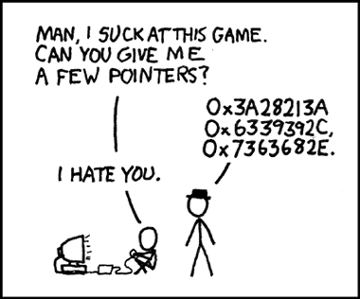
\includegraphics[width=.5\linewidth]{./gfx/xkcd-pointers}
\caption[Pointer im echten Leben]{Pointer im echten Leben. Quelle: \url{https://xkcd.com/138/}}
\end{center}
\end{figure}
\FloatBarrier

\begin{plusbox}
Während C++ ebenfalls Pointer zur Verfügung stellt, die sich dort genauso verhalten wie in der Sprache C, gilt das Paradigma, in C++ \emph{keine} Pointer zu verwenden. C++ kennt andere Konzepte, die Pointer ersetzen (bzw. verstecken) und die helfen, häufige Fehler bei der Arbeit mit Pointern zu vermeiden. Im Rahmen dieses Kurses können leider nur Stichworte genannt werden; sehen Sie dies als Motivation, einen C++-Kurs zu besuchen.

Auch wenn C++-Code \idR keine Verwendung von Pointern macht ist die Kenntnis des Konzepts auch dort sehr wichtig, da der gesamte \enquote{Unterbau} der Sprache auf den hier präsentierten Techniken beruht.
\end{plusbox}

\section{Bitweise Logik und Bit-Shifting} \label{sec:BitwiseOperator}
Für Elektronik-Anwendungen ist es oft nötig, einzelne Schalter an- oder auszuschalten. Meist geschieht dies über eine Zustandsvariable, die an einen \emph{Port} (ein Anschluss, über den Daten fließen können) gesendet wird. Diese Zustandsvariable ist dann \idR eine Ganzzahl-Variable, in der jedes Bit für einen eigenen Schalter steht. Wir benötigen also Mittel, um einzelne Bits zu manipulieren.

Dazu stehen uns die Operatoren \texttt{\~}, \texttt{\&}, \texttt{|}, \texttt{\^}, \texttt{<{}<} und \texttt{>{}>} zur Verfügung.

Die \emph{bitweise Negation} (NOT) \texttt{\~} kehrt jedes Bit um. Betrachten wir die vorzeichenlose 8-Bit-Zahl \texttt{42} (\texttt{00101010}). Das Ergebnis der Negation ist der Wert \texttt{213} (Binärzahl \texttt{11010101}). Als Code lässt sich das wie folgt umsetzen:
\begin{codebox}[Beispiel: Bitweise Negation]
\begin{minted}[linenos]{c}
int main () {
   unsigned char source = 42;
   unsigned char result = ~source;
}
\end{minted}
\end{codebox}

Das \emph{bitweise und} (AND) \texttt{\&} vergleicht die Bits von zwei Werten und setzt das Bit im Ergebnis nur, wenn beide Bits in den Vergleichswerten gesetzt waren (\ie den Wert 1 hatten).

Beim \emph{bitweisen oder} (OR) \texttt{|} werden ebenfalls die Bits von zwei Werten verglichen. Das entsprechende Bit im Ergebnis wird jedoch bereits gesetzt, wenn mindestens eines der Vergleichsbits gesetzt war.

Das \emph{bitweise ausschließliche oder} (XOR) \texttt{\^} arbeitet genauso wie das OR, setzt das Ergebnis-Bit jedoch nur, wenn \emph{genau} eines der Vergleichsbits gesetzt war.

All dies lässt sich in den folgenden Wahrheits-Tabellen ausdrücken:
\begin{codebox}[Wahrheitstabellen: Bitweise Operatoren]
\begin{minted}{text}
     1 1 0 0   12       1 1 0 0   12       1 1 0 0   12
     1 0 1 0   10       1 0 1 0   10       1 0 1 0   10
     - AND -   --       -- OR -   --       - XOR -   --
     1 0 0 0    8       1 1 1 0   14       0 1 1 0    6
\end{minted}
\end{codebox}

Als Code lässt sich das wie folgt umsetzen:
\begin{codebox}[Beispiel: Bitweise Operatoren]
\begin{minted}[linenos]{c}
int main () {
   unsigned char lhs = 12, rhs = 10,
                 and, or, xor;
   and = lhs & rhs;    // =  8
   or  = lhs | rhs;    // = 14
   xor = lhs ^ rhs;    // =  6
}
\end{minted}
\end{codebox}

Die Negation benötigt nur ein \emph{Argument} (Wert, mit dem gearbeitet wird), und wird daher \emph{unärer Operator} genannt. Für AND, OR und XOR sind zwei Werte nötig, weswegen diese als \emph{binäre Operatoren} bezweichnet werden. Die Argumente können auch komplexe Ausdrücke sein, also Ergebnisse von Berechnungen:
\begin{codebox}[Beispiel: Bitweise Operatoren]
\begin{minted}[linenos]{c}
int main () {
   unsigned char result = ~(2 + 7 * (18 & 5));
}
\end{minted}
\end{codebox}

Bitmuster können als ganzes nach links oder rechts verschoben werden. Hierzu dienen die Operatoren \texttt{<{}<} und \texttt{>{}>}.
\begin{codebox}[Beispiel: Bitweise Operatoren]
\begin{minted}[linenos]{c}
int main () {
   unsigned char toLeft  = 170 << 1;
   unsigned char toRight =  85 >> 1;
}
\end{minted}
\end{codebox}
Dies löst folgende Veränderung aus:
\begin{codebox}[Bitshift nach links bzw. nach rechts um jeweils eine Stelle]
\begin{minted}{text}
     1 0 1 0 1 0 1 0   170       0 1 0 1 0 1 0 1    85
     ----- << 1 ----   ---       ----- >> 1 ----   ---
     0 1 0 1 0 1 0 0    84       0 0 1 0 1 0 1 0    42
\end{minted}
\end{codebox}
Bei einem Bitshift nach links werden die Bits am rechten Ende des Bitmusters mit nullen aufgefüllt. Stellen, die am linken Ende über die Registerbreite der aufnehmenden Variable hinaus verschoben werden, gehen verloren. Alles eben gesagte gilt analog für den Bitshift nach rechts.

\begin{hintbox}[Multiplikation mit Zweierpotenzen]
Ein Bitshift um \texttt{n} Stellen nach links entspricht der Multiplikation mit der Zahl $2^{n}$.
Ein Bitshift um \texttt{n} Stellen nach rechts entspricht der Division durch die Zahl $2^{n}$ (Bei Ergebnissen mit Nachkommastelle wird abgerundet). Bitshifts werden schneller durchgeführt als Multiplikationen mit \texttt{*}.

Dies gilt nur für Ganzzahlen, nicht aber für Fließkommazahlen.
\end{hintbox}

\section{Typecasting} \label{sec:Casting}
Es ist gelegentlich notwendig, einen Wert von einem Datentyp in einen anderen umzuwandeln ohne dabei seine Interpretation zu ändern. (Beispielsweise also sollte die Ganzzahl \texttt{3} in die Fließkommazahl \texttt{3.0} umgewandelt werden.) Bei einer solchen Umwandlung ändert sich das Bitmuster, nicht aber der mit diesem Muster dargestellte Wert.

Eine solche Umwandlung wird als \emph{Typecasting} bezeichnet. Die Syntax hierzu ist simpel:
\begin{codebox}[Syntax: Typecasting]
\texttt{(Ziel-Datentyp) Ausdruck}
\end{codebox}
\texttt{Ziel-Datentyp} ist ein beliebiger Datentyp, wie beispielsweise in Anhang \ref{sec:Datatypes} beschrieben. Wie üblich kann \emph{Ausdruck} ein einfacher Wert, eine Variable oder ein komplexer Ausdruck sein.

Ein Grund, den Datentyp zu ändern wurde zum Ende von Abschnitt \ref{sec:OperatorsArithmetic} bereits angeprochen: Operationen wie die Division verhalten sich unterschiedlich, abhängig davon, ob eine Fließkommazahl oder eine Ganzzahl an der Operation beteiligt ist. Solche \emph{Datentyp-spezifischen} Szenarios sind in C sehr häufig.

\begin{codebox}[Beispiel: Typecasting int zu double]
\begin{minted}[linenos]{c}
int main () {
   int x = 7, y = 5;
   double z = (double) x / y;
}
\end{minted}
\end{codebox}

\begin{hintbox}[Reihenfolge der Operationen]
Der Compiler arbeitet \enquote{von links nach rechts}, beachtet aber, dass manche Operationen \enquote{Vorrang} vor anderen haben (\eg Punkt-vor-Strich). Im Obigen Beispiel wird also zuerst der Typecast der Variablen \texttt{x} durchgeführt, und dann der zum \mintinline{c}{double} konvertierte Wert von \texttt{x} durch \texttt{y} geteilt. Damit erhält \texttt{z} den Wert \texttt{1.2}.

Im folgenden Beispiel dagegen erhält \texttt{z} den Wert 1.0:
\begin{codebox}[Beispiel: Fehlerhaftes Typecasting int zu double]
\begin{minted}[linenos]{c}
int main () {
   int x = 7, y = 5;
   double z = (double) (x / y);
}
\end{minted}
\end{codebox}
Durch die Klammern interpretiert der Compiler Zeile 3 als: \enquote{Caste das Ergebnis von \texttt{x / y} zu \mintinline{c}{double}}. Da das Ergebnis von \texttt{x / y} aus der Division zweier \mintinline{c}{int}-Werte hervorgeht, wird hier gerundet und \texttt{z} erhält den (\idR falschen) Wert \texttt{1.0}.
\end{hintbox}

\section{Hierarchie der Operatoren} \label{sec:OperatorHierarchy}
Ausdrücke werden vom Compiler \enquote{von links nach rechts} ausgewertet, wobei die Vorrangigkeit mancher Operatoren beachtet wird. Die Vorrangigkeit kann Tabelle \ref{tab:OperatorPrecedence} im Anhang entnommen werden. Wo immer Unsicherheiten bestehen, kann durch Setzen von (runden Klammern) Sicherheit geschaffen werden.

\section{Zahlenformate -- Hexadezimalsystem} \label{sec:NumSystems}
Gleich zu Beginn dieses Kurses in Abschnitt \ref{sec:BinaryNumbers} haben wir das \emph{Binärsystem} (oder auch \emph{Dualsystem}) kennen gelernt, das neben dem uns vertrauten \emph{Dezimalsystem} steht\footnote{Übrigens: Das Dezimalsystem wäre völlig unbrauchbar, wenn der Mensch nicht zufällig zehn Finger hätte. (Kalenderspruch)}. Nach der dort gezeigten Idee lassen sich Zahlen in beliebigen \emph{Zahlensystemen} bzw. mit beliebiger \emph{Basis} (also Anzahl von verschiedenen Ziffern im Zahlensystem) darstellen. Von besonderer Bedeutung ist das \emph{Hexadezimalsystem} mit 16 Ziffern:

\begin{center}
\texttt{0 1 2 3 4 5 6 7 8 9 A B C D E F}
\end{center}

Um eine Zahl als \emph{hexadezimal} zu kennzeichnen wird häufig der Präfix \texttt{0x} vorangestellt. Der Ausdruck \texttt{0x10} beschreibt also die \emph{Dezimalzahl} 16\footnote{Andere verbreitete Schreibweisen sind \texttt{10h}, \texttt{$10_{16}$} oder \texttt{$10_{hex}$}}. Groß- und Kleinschreibung wird hier nicht unterschieden, es gilt \texttt{0xab} = \texttt{0XAB}.

Die weiteren Informationen in diesem Abschnitt sind für besonders interessierte KursteilnehmerInnen gedacht und müssen für den Kurserfolg nicht im Detail verstanden werden. Sie werden diese Idee aber in der IT-Welt immer wieder antreffen und Nutzen aus dem Verständnis ziehen.

Das Hexadezimalsystem wird immer da verwendet, wo die \emph{Registerbreite} eines Wertes im Speicher Relevanz hat\footnote{Historische Bedeutung hat in diesem Kontext auch noch das \emph{Oktalsystem}, das die Ziffern \texttt{0..7} verwendet. Heute lebt es fast nur noch in dem Witz fort: \emph{Why do programmers confuse Halloween and Christmas? Because Oct 31 = Dec 25...}}. Wir haben bereits gehört, dass ein Computer nur Einheiten zu jeweils 8 Bit behandeln kann. Ein Byte, also eine Gruppe von 8 Bit erlaubt, wie in Abschnitt \ref{sec:Datawidth} erwähnt, 256 verschiedene Werte. Im Hexadezimalsystem wird daraus der \enquote{runde} Wert \texttt{0x100}. Ähnlich ist die Zahl der mit 16 Bit darstellbaren Zahlen gleich \texttt{0x10000} und für 32 bit erhalten wir \texttt{0x100000000} verschiedene Möglichkeiten. Dies ist kein Zufall -- Die Zahl 16 (also die Basis des Hexadezimalsystems) ist eine Potenz der Zahl 2 (also der Basis des Binärsystems). Es besteht eine \enquote{direkte Verwandschaft} zwischen Binärzahlen und Hexadezimalzahlen.

Eine Zahl, die mit $n$ Bit dargestellt wird, kann also mit $\frac{n}{4}$ Hexadezimal-Ziffern geschrieben werden. Dies ist offensichtlich praktischer als lange Ketten von 1en und 0en zu schreiben.

\begin{hintbox}[Farben als Hexadezimal-Werte]
In der Computertechnik werden Farben häufig mit \emph{Hex-Codes} beschrieben. Dies sind sechsstellige Kombinationen aus Ziffern und den Buchstaben A bis F. Tatsächlich sind diese Codes drei aneinander gereihte Hexadezimalzahlen. Diese beschreiben jeweils den Rot-, Grün- und Blau-Anteil einer Farbe. Der Dezimalwert 255 (bzw. die Hexadezimalzahl \texttt{0xFF}) beschreibt dabei \enquote{volle Intensität}, 0 (oder \texttt{0x00} dagegen sagt aus, von der Teilfarbe kommt kein Beitrag. Damit kann die Farbe Orange dann ausgedrückt werden als \texttt{0xFF7F00}: Volle Intensität Rot (\texttt{FF}), halbe Intensität Grün (\texttt{7F}) und Blau-Anteil 0 (\texttt{00}).

Siehe auch \url{https://de.wikipedia.org/wiki/Additive_Farbmischung}
\end{hintbox}

\begin{hintbox}[Zweier-Potenzen in der Computerwelt]
\emph{Alles} in der Computertechnik ist um Potenzen der Zahl 2 aufgebaut. Wir finden 32bit und 64bit-Betriebssysteme, USB-Sticks mit 2, 4, 8 oder 16 GB, oder sogar Bildschirmauflösungen wie 1024x768 Pixel. Diese Zahlen kommen derartig häufig vor, dass sie von TechnikerInnen bereits als \enquote{runde Zahlen} wahrgenommen werden. So feierte beispielsweise Randall Munroe, Author des Webcomics \href{https://www.xkcd.com/}{xkcd} seinen eintausendsten Strip mit dieser Veröffentlichung:

\begin{center}
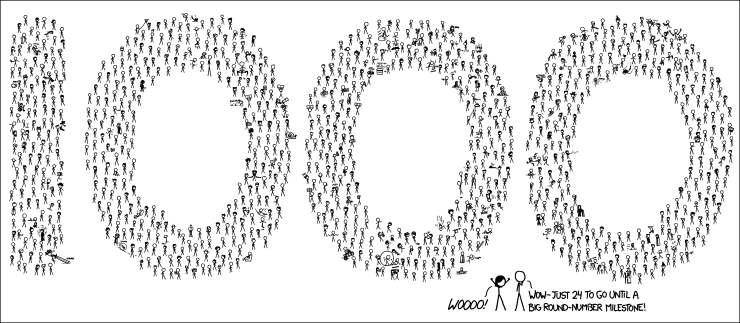
\includegraphics[width=.9\linewidth]{./gfx/xkcd-1000}
\end{center}
\captionof{figure}
	[Dezimale und Binäre runde Zahlen]
	{Dezimale und Binäre runde Zahlen. Quelle: \url{https://www.xkcd.com/1000/}}
\end{hintbox}
	\chapter{Dateneingabe} \label{chp:Input}
\epigraph{On two occasions I have been asked, \enquote{Pray, Mr. Babbage, if you put into the machine wrong figures, will the right answers come out?} ... I am not able rightly to apprehend the kind of confusion of ideas that could provoke such a question.}{Charles Babbage, Passages from the Life of a Philosopher}

In den letzten Kapiteln haben wir gesehen, wie wir in der Sprache C einfache Berechnungen realisieren können. Die Daten, mit denen gerechnet wurde, standen dabei jedoch schon vor Start des Programmes fest. Im folgenden sollen einfache Mittel vorgestellt werden, die Usereingaben und damit Interaktivität ermöglichen.

\section{Dateneingabe mit \texttt{scanf}}
Die Funktion \texttt{scanf} dient dazu, Tastatureingaben von der Konsole einzulesen, in verschiedene Datenformate umzurechnen und dann als solche im Speicher abzulegen. Die Funktion ist deklariert im Header \texttt{stdio.h} (wie auch \texttt{printf}). Betrachten wir das folgende Beispiel:

\begin{codebox}[Beispiel: Eine Ganzzahl mit \texttt{scanf} einlesen]
\begin{minted}[linenos]{c}
#include <stdio.h>

int main () {
   int Ganzzahl = -1;

   printf("Bitte geben Sie eine Ganzzahl ein:\n");
   scanf("%d", &Ganzzahl);

   printf("Ihre Eingabe war: %d\n", Ganzzahl);
}
\end{minted}
\end{codebox}

Wie gewohnt haben wir den Header \texttt{stdio.h} in Zeile 1 geladen und können nun die Funktionen \texttt{printf} und \texttt{scanf} verwenden. In Zeile 4 deklarieren wir eine Variable \texttt{Ganzzahl} und initialisieren sie mit dem Startwert \texttt{-1}. Nach der Aufforderung an den Benutzer unseres Programms (Zeile 6) lesen wir jetzt mit \texttt{scanf} einen Wert in den Speicher:

Ähnlich wie \texttt{printf} nimmt \texttt{scanf} als erstes Argument einen \emph{Formatstring} an. Dieser beschreibt, welche Art von Werten erwartet wird, und benutzt dieselben Formatierungszeichen wie \texttt{printf} (siehe Tabelle \ref{tab:FormatIn} im Anhang für Details). Das folgende Argument ist die \emph{Adresse, an die der eingelesene Wert geschrieben werden soll}. Wir benutzen den Adress-Operator \texttt{\&}, um dem Compiler mitzuteilen, dass der eingelesene Wert an der Adresse der Variable \texttt{Ganzzahl} abgelegt werden soll. Hier überschreiben wir also den Wert von \texttt{Ganzzahl} mit der Eingabe des Users, interpretiert als \mintinline{c}{int} (vorgegeben durch das Formatierungszeichen \texttt{\%d}).

In der Ausführung kann dies so aussehen:
\begin{cmdbox}[Ausführungsbeispiel: Eine Ganzzahl mit \texttt{scanf} einlesen]
\begin{minted}{text}
Bitte geben Sie eine Ganzzahl ein:
42
Ihre Eingabe war: 42
\end{minted}
\end{cmdbox}

\begin{hintbox}[Unterschied von Zahlenwerten und Text mit Ziffern]
Bitte beachten Sie: Die User-Eingabe war ein Text, bestehend aus zwei \emph{Zeichen} (eben der \texttt{4} und der \texttt{2}). Diese beiden Zeichen werden von \texttt{scanf} erst zu dem Zahlenwert $42$ zusammengesetzt und schließlich als \mintinline{c}{int}-Wert im Speicher abgelegt. Das \emph{Bitmuster} des \enquote{\emph{Textes}} \texttt{42} ist ein anderes als das der \emph{Zahl} $42$. Wir werden bald Fälle sehen, in denen dieser Unterschied von Bedeutung ist. Um diese Denkweise bereits jetzt einzuüben, mache ich Sie hier auf den Gedanken aufmerksam.
\end{hintbox}

Beim Einlesen versucht \texttt{scanf}, die User-Eingaben im Kontext des angegebenen Datentyps zu interpretieren. Passen die Eingaben nicht zum Typ, so werden sie \idR ignoriert, können aber auch unvorhergesehene Ergebnisse liefern. Hierzu zwei Laufzeit-Beispiele zum obigen Code:

\begin{cmdbox}[Ausführungsbeispiel: Eine Ganzzahl mit \texttt{scanf} einlesen]
\begin{minted}{text}
Bitte geben Sie eine Ganzzahl ein:
12.3
Ihre Eingabe war: 12
\end{minted}
\end{cmdbox}

Während der Code einen Ganzzahl-Wert erwartet (\texttt{\%d}), hat der User eine Fließkommazahl eingegeben. \texttt{scanf} ignoriert den Nachkomma-Anteil und speichert nur den Wert \texttt{12}.

\begin{cmdbox}[Ausführungsbeispiel: Eine Ganzzahl mit \texttt{scanf} einlesen]
\begin{minted}{text}
Bitte geben Sie eine Ganzzahl ein:
a
Ihre Eingabe war: -1
\end{minted}
\end{cmdbox}
Der Buchstabe \texttt{a} kann nicht als Ganzzahl interpretiert werden. Der Startwert \texttt{-1} wird nicht überschrieben.

\begin{hintbox}[Fehlerhafte Usereingaben erwarten]
Als ProgrammiererIn sollten Sie immer davon ausgehen, dass die Anwender Ihrer Programme Fehler machen werden. Diese Fehler sollen von Ihrem Programm \emph{abgefangen} werden können. Wir werden in Kapitel \ref{chp:Conditions} lernen, wie wir Teile unseres Codes nur unter bestimmten Bedingungen ausführen lassen. Um solche Bedingungen zu formulieren müssen jedoch geeignete (definierte) Startbedingungen vorliegen. Im Beispiel oben könnte geprüft werden, ob der Wert von \texttt{Ganzzahl} nach dem Eingabeversuch immer noch \texttt{-1} ist und eine entsprechende \emph{Fehlerbehandlung} für diesen Fall nachgeschalten werden. Natürlich ist es möglich, dass ein Anwender genau den Wert \texttt{-1} eingeben will. Welche Startwerte sinnvoll sind und wie die Fehlerbehandlung aussehen kann, hängt vom jeweiligen Kontext ab. Behalten Sie in jedem Fall den Gedanken, dass fehlerhafte Usereingaben häufig sind und von Ihnen \enquote{vorhergesehen} werden sollten. Aus diesem Grund ist es sinnvoll hier einen Startwert für die Variable \texttt{Ganzzahl} festzulegen, auch wenn dieser quasi sofort überschrieben wird.
\end{hintbox}

Betrachten wir weiter das folgende Beispiel:

\begin{warnbox}[Beispiel: Fehler bei \texttt{scanf}: Falsche Typisierung, leftupper=7mm]
\begin{minted}[linenos]{c}
#include <stdio.h>

int main () {
   int Ganzzahl = -1;

   printf("Bitte geben Sie eine Ganzzahl ein:\n");
   scanf("%f", &Ganzzahl);

   printf("Ihre Eingabe war: %d\n", Ganzzahl);
}
\end{minted}
\end{warnbox}

Gegenüber dem Beispiel zu Eingang des Kapitels hat sich lediglich Zeile 7 geändert: Statt mit \texttt{\%d} einen \mintinline{c}{int} zu lesen, fordern wir nun mit \texttt{\%f} dazu auf, eine \mintinline{c}{float}-Variable zu lesen. Diese wird wieder an den Speicherort der Variablen \texttt{Ganzzahl} geschrieben, die jedoch vom Typ \mintinline{c}{int} ist!

Der Compiler kann diesen (fehlerhaften) Code umsetzen, gibt aber eine entsprechende Warnung aus:

\begin{cmdbox}[Compiler-Warnung: Fehlerhafte Typisierung mit \texttt{scanf}]
\begin{minted}{text}
myProgram.c: In function ‘main’:
myProgram.c:7:12: warning: format ‘%f’ expects argument of type ‘float *’, but
argument 2 has type ‘int *’ [-Wformat=]
    scanf("%f", &Ganzzahl);
           ~^   ~~~~~~~~~
           %d
\end{minted}
\end{cmdbox}

Ähnlich wie bei \texttt{printf} markiert der Compiler die relevante Stelle und schlägt vor, mit \texttt{\%d} einzulesen. Es handelt sich aber nur um eine Warnung; der Compiler kann \enquote{funktionierenden} Maschinencode erzeugen. Ebenso wie auch bereits zu Ende von Abschnitt \ref{sec:formattedOutput} erklärt, ist das Ergebnis dieser Ausführung aber \enquote{unsinnig}:

\begin{cmdbox}[Ausführungsbeispiel: Fehlerhafte Typisierung mit \texttt{scanf}]
\begin{minted}{text}
Bitte geben Sie eine Ganzzahl ein:
1
Ihre Eingabe war: 1065353216
\end{minted}
\end{cmdbox}

Noch schwerwiegender wird der Fehler, wenn wir statt dem Formatierungscode \texttt{\%f} für \mintinline{c}{float} mit \texttt{\%lf} einen \mintinline{c}{double}-Wert einlesen.
Variablen des Typs \mintinline{c}{int} und \mintinline{c}{float} sind 32 Bit breit\footnote{zumindest auf den heute üblichen Rechnern}. Ein \mintinline{c}{double}-Wert dagegen ist 64 Bit breit. Beim Einlesen wird also \enquote{über die Grenzen des reservierten Speicherbereichs hinaus geschrieben}. Der Effekt hiervon ist absolut \emph{undefiniertes Verhalten}. Im \enquote{besten Fall} wird der \enquote{zu viel beschriebene} Speicherplatz nicht benötigt und das Programm läuft ohne größere Nebeneffekte weiter. Es ist aber auch möglich, dass in andere reservierte Bereiche hinein geschrieben wird (\emph{bleeding}) und so andere Variablen geändert werden:

\begin{warnbox}[Beispiel: Fehler bei \texttt{scanf}: bleeding, leftupper=7mm]
\begin{minted}[linenos]{c}
#include <stdio.h>

int main () {
   int x = 10;
   int y = 10;  // Adresse von y entspricht Adresse von x + 4 !

   printf("Bitte geben Sie eine Zahl ein:\n");
   scanf("%lf", &x);

   printf("(x, y) = (%d, %d)\n", x, y);
}
\end{minted}
\end{warnbox}

Die beiden Variablen \texttt{x} und \texttt{y} werden im Speicher direkt aufeinander folgend angelegt. Schreiben wir über die Grenzen von \texttt{x} hinaus, so ändern wir auch \texttt{y}:

\begin{cmdbox}[Ausführungsbeispiel: Fehler bei \texttt{scanf}: bleeding]
\begin{minted}{text}
Bitte geben Sie eine Zahl ein:
1
(x, y) = (0, 1072693248)
\end{minted}
\end{cmdbox}

Im schlimmsten Fall resultiert unvorhersagbares Laufzeit-Verhalten oder Absturz des Programms wegen Speicherzugriffsfehler (\emph{Segmentation fault} bzw. kurz \emph{Segfault}).

\begin{warnbox}[Typisierung]
Achten Sie extrem genau auf richtige Typisierung wann immer Sie mit Adressen (Operator \texttt{\&}) arbeiten. Fehler dieser Art sind in großen Projekten extrem schwierig zu finden und führen zu instabilem Code. Beachten Sie insbesondere alle Warnungen, die der Compiler ausgibt.
\end{warnbox}

Wie bei \texttt{printf} darf der Formatstring bei \texttt{scanf} auch mehrere Platzhalter enthalten, die dann durch Leerstellen voreinander getrennt werden. Der User hat dann die Möglicheit, alle Werte \enquote{in einer Zeile} einzugeben, und diese durch Leerzeichen zu trennen, oder jeden Wert in eine eigene Zeile zu setzen.

\begin{codebox}[Beispiel: Eingabe mehrerer Werte mit \texttt{scanf}]
\begin{minted}[linenos]{c}
#include <stdio.h>

int main () {
   int    x = 0;
   double y = 0;

   printf("Bitte geben Sie eine Ganzahl und eine Fließkommazahl ein:\n");
   scanf("%d %lf", &x, &y);

   printf("(x, y) = (%d, %lf)\n", x, y);
}
\end{minted}
\end{codebox}

\begin{cmdbox}[Ausführungsbeispiel: Eingabe mehrerer Werte mit \texttt{scanf}]
\begin{minted}{text}
Bitte geben Sie eine Ganzahl und eine Fließkommazahl ein:
1 1.5
(x, y) = (1, 1.500000)
\end{minted}
\end{cmdbox}

Jeder Wert wird einzeln interpretiert; natürlich muss die Reihenfolge der Usereingaben der Reihenfolge der Platzhalter in der \texttt{scanf}-Anweisung entsprechen.

\begin{hintbox}[User-Freundliches Verhalten]
Die Erfahrung zeigt, dass User bei der Eingabe mehrerer Werte in einem Block häufig Fehler machen. Ich empfehle, jeweils nur einen einzelnen Wert einlesen zu lassen, und vor jedem \texttt{scanf}-Befehl einen Hinweis mit \texttt{printf} auszugeben, welcher Wert erwartet wird.
\end{hintbox}

\begin{warnbox}[Adressen bei \texttt{scanf}]
Wichtig ist, dass \texttt{scanf} eine \emph{Adresse} erwartet. Ein häufiger Fehler ist es, den Adress-Operator \texttt{\&} zu vergessen wie im folgenden Beispiel:

\begin{warnbox}[Beispiel: Eine Ganzzahl mit \texttt{scanf} einlesen, leftupper=7mm]
\begin{minted}[linenos]{c}
#include <stdio.h>

int main () {
   int Ganzzahl = 0;

   printf("Bitte geben Sie eine Ganzzahl ein:\n");
   scanf("%d", Ganzzahl);

   printf("Ihre Eingabe war: %d\n", Ganzzahl);
}
\end{minted}
\end{warnbox}

Hier wird versucht, an die Adresse zu schreiben, die gerade in der Variablen \texttt{Ganzzahl} gespeichert ist -- also an die Adresse \texttt{0}. Dies ist ein verbotener Zugriff und endet daher in einem Programmabsturz.

Der Compiler gibt eine entsprechende Warnung aus:
\begin{cmdbox}[Compilerwarnung: Ungültige Adresse übergeben]
\begin{minted}{text}
myProgram.c: In function ‘main’:
myProgram.c:7:12: warning: format ‘%d’ expects argument of type ‘int *’,
but argument 2 has type ‘int’ [-Wformat=]
    scanf("%d", Ganzzahl);
           ~^
\end{minted}
\end{cmdbox}

und die Programmausführung stoppt mit einem \emph{Segfault} bzw. Speicherzugriffsfehler:

\begin{cmdbox}[Ausführungsbeispiel: Ungültige Adresse übergeben]
\begin{minted}{text}
Bitte geben Sie eine Ganzzahl ein:
1
Speicherzugriffsfehler (Speicherabzug geschrieben)
\end{minted}
\end{cmdbox}
\end{warnbox}

\section{Ausblick: Eingabe in C++}
\begin{plusbox}
Wie schon bei der Textausgabe kann alles oben gesagte auch in C++ angewandt werden. Es bietet sich jedoch an, auch hier wieder \emph{Streams} zu verwenden. Das folgende Beispiel zeigt, wie mit den Mitteln der \texttt{iostream}-Bibliothek Werte eingelesen werden können.

\begin{codebox}[Beispiel: Eingabe mehrerer Werte mit \texttt{scanf}]
\begin{minted}[linenos]{c++}
#include <iostream>

int main () {
   int    x = 0,
          y = 0;
   double z = 0;

   std::cout << "Bitte geben Sie eine Ganzahl ein:" << std::endl;
   std::cin  >> x;

   std::cout << "Bitte geben Sie eine Ganzahl ";
   std::cout << "und eine Fließkommazahl ein:" << std::endl;
   std::cin  >> y >> z;

   std::cout << "Ihre erste Eingabe war: " << x << std::endl;
   std::cout << "Ihre zweite Eingabe war: ";
   std::cout << y << ", " << z << std::endl;
}
\end{minted}
\end{codebox}

Wir verwenden also den \emph{Eingabestream} \texttt{std::cin}. Aus diesem können mit dem Operator \texttt{>{}>} Werte \enquote{angefordert} werden, die nach denselben Regeln interpretiert werden, wie dies schon bei \texttt{scanf} besprochen wurde. Jedoch entfällt die Notwendigkeit eines Format-Strings; der Datentyp wird \emph{automatisch} aus dem Typ der Variablen ermittelt, die hinter \texttt{>{}>} steht. Achtung: Hier werden die Variablen selbst, nicht ihre Adressen aufgeführt; der Operator \texttt{\&} entfällt!

Mehr zum Thema unter \url{https://en.cppreference.com/w/cpp/io/cin}.
\end{plusbox}

	\chapter{Bedingungen} \label{chp:Conditions}
\epigraph{In any moment of decision, the best thing you can do is the right thing, the next best thing is the wrong thing, and the worst thing you can do is nothing.}{Theodore Roosevelt}

Bis hierhin haben wir Programme mit \emph{linearem} Verlauf geschrieben: unsere Befehle werden von oben nach unten ohne Auslassungen oder Sprünge bearbeitet. Hier nun wollen wir erste Strukturen einführen, die den \emph{Programmfluss} ändern: Wir wollen bestimmte Code-Teile nur dann ausführen, wenn bestimmte \emph{Bedingungen} erfüllt sind.

\section{Wahrheitswerte} \label{sec:truthvalues}
Mathematischen Ausdrücken können \emph{Wahrheitswerte} zugeordnet werden. Diese Wahrheitswerte sagen aus, ob es sich um eine \enquote{wahre} oder \enquote{falsche} Aussage handelt. Ein Beispiel für einen solchen Ausdruck ist:
\begin{center}
\mintinline{c}{1 + 5 * 8 + 1 == 42}
\end{center}
Der Wahrheitswert dieses Ausdrucks ist offensichtlich \emph{wahr} (bzw. \emph{true}).

Beachten Sie bitte, dass für den \emph{Vergleich} zweier Zahlen das \emph{doppelte Gleichheitszeichen} \texttt{==} verwendet wird. Das einfache Gleichheitszeichen \texttt{=} dient ausschließlich der \emph{Wertzuweisung} an Variablen.

Tabelle \ref{tab:OperatorsComparison} listet Vergleichsoperatoren auf.
\begin{table}[h!]
	\newcolumntype{C}{>{         \centering\arraybackslash} p{.25\linewidth}}
	\newcolumntype{O}{>{\ttfamily\centering\arraybackslash} p{.20\linewidth}}
\begin{center}
\begin{tabularx}
	{.95\linewidth}
	{CO|CO}
\toprule[1pt]

	Vergleich           & \normalfont Zeichen  &
	Vergleich           & \normalfont Zeichen
\tabcrlf

	Gleichheit          & ==                   &  Ungleichheit         & != \\
	Kleiner als         & <                    &  Größer als           & >  \\
	Kleiner oder gleich & <=                   &  Größer oder gleich   & >= \\

\bottomrule[1pt]
\end{tabularx}
\end{center}
\caption{Vergleichsoperatoren in C}\label{tab:OperatorsComparison}
\end{table}

Da es nur zwei Wahrheitswerte gibt (\emph{wahr} und \emph{falsch}, bzw. \emph{true} und \emph{false}) wird im Prinzip nur ein einzelnes Bit benötigt, um einen solchen Wahrheitswert zu speichern. Ein Prozessor kann jedoch nur Gruppen zu mindestens 8 Bit behandeln, nicht aber einzelne Bits. Für uns sind Wahrheitswerte daher Ganzzahl-Werte, wie etwa \mintinline{c}{int}s. In der Tat lassen sich solche Wahrheitswerte speichern und ausgeben:

\begin{codebox}[Beispiel: Speichern und Ausgabe von Wahrheitswerten]
\begin{minted}[linenos]{c}
#include <stdio.h>

int main () {
   int    true   = 1 + 1 == 2,
          false  = 1 + 1 != 2;

   printf("Wert von 'true' : %d\n", true );
   printf("Wert von 'false': %d\n", false);
}
\end{minted}
\end{codebox}

Die Ausgabe hierzu lautet:

\begin{cmdbox}[Ausführungsbeispiel: Speichern und Ausgabe von Wahrheitswerten]
\begin{minted}{text}
Wert von 'true' : 1
Wert von 'false': 0
\end{minted}
\end{cmdbox}

Da eine \mintinline{c}{int}-Variable mehr Werte als \texttt{0} und \texttt{1} halten kann, interpretiert man alle von null verschiedenen Werte als \emph{wahr}.

Selbstverständlich können Ausdrücke, die zu Wahrheitswerten ausgewertet werden, auch Variablen enthalten. Es kann sogar mit ihnen gerechnet werden (auch wenn dies nur selten sinnvoll ist).

\begin{codebox}[Beispiel: Rechnen mit Wahrheitswerten]
\begin{minted}[linenos]{c}
#include <stdio.h>

int main () {
   int x     = 17,
       truth = (x > 5) + (x < 5) + (x == 17);

   printf("%d wahre Ausdrücke.\n", truth);
}
\end{minted}
\end{codebox}

\begin{cmdbox}[Ausführungsbeispiel: Rechnen mit Wahrheitswerten]
\begin{minted}{text}
2 wahre Ausdrücke.
\end{minted}
\end{cmdbox}

Nacheinander werden die drei Vergleiche \texttt{x > 5}, \texttt{x < 5} und \texttt{x == 17} ausgewertet (jeweils zu \texttt{1}, \texttt{0}, und \texttt{1}) und dann aufsummiert. Diese Summe wird in der normalen \mintinline{c}{int}-Variable \texttt{truth} gespeichert.

\begin{warnbox}[Symbole \texttt{true} und \texttt{false}]
Die Symbole \texttt{true} und \texttt{false} sind zwar nach keinem bisherigen C-Standard definiert; in vielen Bibliotheken sind diese Symbole aber mit den Werten \texttt{1} bzw. \texttt{0} definiert, und sollten daher auch ausschließlich im Sinne von Wahrheitswerten verwendet werden. Vermeiden Sie nach Möglichkeit die Verwendung der Symbole als Variablen ganz.

In C++ sind sowohl \mintinline{c++}{true} als auch \mintinline{c++}{false} fester Bestandteil der Sprache und können nicht als Variablennamen vergeben werden.
\end{warnbox}
\section{Bedingte Ausführung von Code: \mintinline{c}{if}}
Mit dem Konstrukt \mintinline{c}{if} lassen sich \emph{Wenn-Dann-Blöcke} erstellen: WENN \emph{Bedingung erfüllt}, DANN \emph{führe Anweisungen aus}. Bedingungen werden als mathematische Ausdrücke formuliert, die als erfüllt gelten, wenn ihr Wahrheitswert \emph{true} ist. \emph{Anweisungen} kann ein einzelner Befehl oder eine ganze Reihe von Befehlen sein. In der einfachsten Form sieht ein \mintinline{c}{if}-Block so aus:

\begin{codebox}[Syntax: Einfacher \texttt{if}-Block]
\begin{minted}{c}
if (Bedingung) {
   ... Anweisungen ...
}
\end{minted}
\end{codebox}

Im Kontext eines vollständigen Programms kann dies so aussehen:

\begin{codebox}[Beispiel: Einfacher \texttt{if}-Block]
\begin{minted}[linenos]{c}
#include <stdio.h>

int main () {
   int foo = 0;

   printf("Bitte geben Sie eine Ganzzahl ein:\n");
   scanf("%d", &foo);

   if (foo % 2 == 0) {
      printf("%d ist eine gerade Zahl.\n", foo);
   }

   printf("Sie haben %d eingegeben.\n", foo);
}
\end{minted}
\end{codebox}

Die Anweisung in Zeile 10 wird nur ausgeführt, wenn der Rest der Division von \texttt{foo} durch \texttt{2} gleich null ist, also wenn der Wert der Variablen gerade ist. Unabhängig vom Ausgang dieser Entscheidung wird Zeile 13 in jedem Fall ausgeführt.

Wenn auf die Bedingung nur eine einzelne Anweisung folgt (wie im obigen Beispiel), so können die \{geschweiften Klammern\} auch entfallen. Der folgende Code führt also zum selben Ergebnis:

\begin{codebox}[Beispiel: Einzeiliger \texttt{if}-Block]
\begin{minted}[linenos]{c}
#include <stdio.h>

int main () {
  int foo = 0;
  printf("Bitte geben Sie eine Ganzzahl ein:\n");
  scanf("%d", &foo);

  if (foo % 2 == 0)
    printf("%d ist eine gerade Zahl.\n", foo);

  printf("Sie haben %d eingegeben.\n", foo);
}
\end{minted}
\end{codebox}

\begin{warnbox}[Fehlerquelle fehlende Klammern]
Es mag praktisch erscheinen, die geschweiften Klammern bei einzeiligen \mintinline{c}{if}-Blocks nicht zu setzen. Nicht selten ergänzt man sein Programm im Laufe eines Projekts aber noch. Hängt man neue Befehle an einen \mintinline{c}{if}-Block an, so muss man diese Klammern natürlich nachsetzen. Dies wird oft vergessen. Betrachten Sie folgenden Code:

\begin{warnbox}[Beispiel: Fehlerhafter \texttt{if}-Block durch fehlende Klammern, leftupper=7mm]
\begin{minted}[linenos]{c}
#include <stdio.h>

int main () {
   int foo = 0;

   printf("Bitte geben Sie eine Ganzzahl ein:\n");
   scanf("%d", &foo);

   if (foo % 2 == 0)
      printf("%d ist eine gerade Zahl.\n", foo);
      printf("%d ist durch 2 teilbar.\n", foo);

   printf("Sie haben %d eingegeben.\n", foo);
}
\end{minted}
\end{warnbox}

Die Ausgabe in Zeile 10 findet nur statt, wenn \texttt{foo} einen geraden Wert hält; Zeile 11 dagegen wird fälschlicherweise \emph{immer} ausgeführt. Die Code-Einrückung -- eigentlich ein Zeichen guten Stils -- kaschiert diesen Fehler noch mehr. Ich rate daher dazu, \emph{immer} Klammern zu setzen. Richtig müsste der \mintinline{c}{if}-Block also lauten:

\begin{codebox}[Beispiel: Korrekter mehrzeiliger \texttt{if}-Block]
\begin{minted}[linenos,firstnumber=9]{c}
   if (foo % 2 == 0) {
      printf("%d ist eine gerade Zahl.\n", foo);
      printf("%d ist durch 2 teilbar.\n", foo);
   }
\end{minted}
\end{codebox}
\end{warnbox}

Mit dem Schlüsselwort \mintinline{c}{else} kann der \mintinline{c}{if}-Block noch um Anweisungen ergänzt werden, die nur ausgeführt werden sollen, wenn die Bedingung gerade \emph{nicht} erfüllt war:

\begin{codebox}[Beispiel: \texttt{if-else}-Block]
\begin{minted}[linenos]{c}
#include <stdio.h>

int main () {
  int foo = 0;
  printf("Bitte geben Sie eine Ganzzahl ein:\n");
  scanf("%d", &foo);
}
\end{minted}
\end{codebox}
%
\begin{codebox}[]
\begin{minted}[linenos, firstnumber=last]{c}
  if (foo % 2 == 0) {
    printf("%d ist eine gerade Zahl.\n", foo);
  } else {
    printf("%d ist eine ungerade Zahl.\n", foo);
  }
}
\end{minted}
\end{codebox}

\begin{hintbox}[Stil: Einrückungen und Position der Klammern]
Gute Programmierer sind sich einig, dass Einrückungen fester Bestandteil von gutem Code sind. Ohne diese verliert man in auch nur wenig komplexen Projekten schnell den Überblick und macht unnötige Fehler. Hier aber endet auch schon die Einigkeit; es gibt keine allgemein anerkannte \enquote{richtige Art, Code einzurücken}. Tabulatoren oder Leerzeichen, zwei oder vier Zeichen pro Einrückung, oder auch die Position der Klammern -- verschiedenste Varianten werden gelebt und kontrovers und teilweise sehr emotional diskutiert, wie Abbildung \ref{fig:IndentStyle} zeigt.

Sie sind also frei, Ihren Stil selbst zu definieren, sollten dabei aber zwei Regeln einhalten:
\begin{itemize}
\item Halten Sie Ihren Code einheitlich, \ie behalten Sie den Einrückungs-Stil über ein gesamtes Projekt konsistent.
\item Ändern Sie niemals den Einrückungs-Stil ihrer KollegInnen.
\end{itemize}
\end{hintbox}

\begin{figure}
	\href{http://www.sandraandwoo.com/2015/04/13/0674-there-are-10-types-of-programmers/}{
		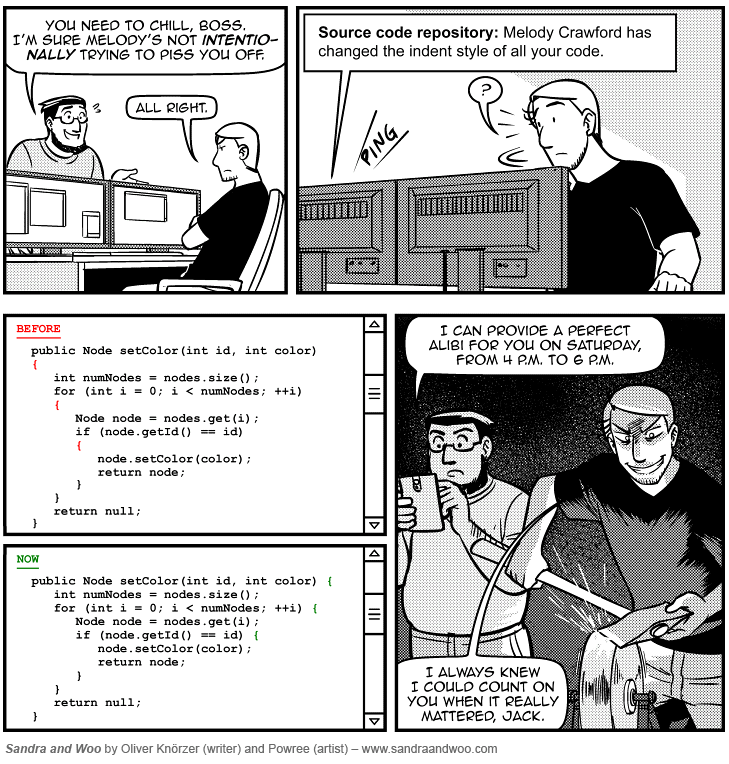
\includegraphics[width=\linewidth]{./gfx/SW-indent-style}
	}
	\caption{Ein realistisches Szenario} \label{fig:IndentStyle}
\end{figure}

\mintinline{c}{if}-Blöcke dürfen nahezu beliebig tief verschachtelt werden\footnote{Der Standard aus dem Jahre 1999 verpflichtet die Programmierer von C-Compilern zwar \enquote{nur} dazu, mindestens 127 Ebenen (256 für C++) zu unterstützen; im Falle des gcc bricht der Kompiliervorgang aber erst nach 6199 Ebenen mit Fehlermeldung ab.}. Das folgende Beispiel prüft also zuerst, ob eine eingegebene Zahl positiv war, und nur für positive Zahlen die \emph{Parität} (die Eigenschaft, gerade oder ungerade zu sein).

\begin{codebox}[Beispiel: Verschachtelter \texttt{if-else}-Block]
\begin{minted}[linenos]{c}
#include <stdio.h>

int main () {
   int foo = 0;

   printf("Bitte geben Sie eine Ganzzahl ein:\n");
   scanf("%d", &foo);

   if (foo > 0) {
      if (foo % 2 == 0) {
         printf("%d ist eine gerade Zahl.\n"  , foo);
      } else {
         printf("%d ist eine ungerade Zahl.\n", foo);
      }
   } else {
      printf("%d ist eine ungültige Zahl.\n"  , foo);
   }
}
\end{minted}
\end{codebox}

Spätestens an diesem Beispiel erkennen Sie, weshalb auf Einrückung so viel Wert gelegt wird. Sehen Sie sich zum Vergleich auch das folgende -- syntaktisch korrekte -- Beispiel ohne Einrückungen an:

\begin{warnbox}[Schlechter Stil: Code mit mehreren Hierarchie-Ebenen ohne Einrückungen, leftupper=7mm]
\begin{minted}[linenos]{c}
#include <stdio.h>
int main () {
int foo = 0;
printf("Bitte geben Sie eine Ganzzahl ein:\n");
scanf("%d", &foo);
if (foo > 0) {
if (foo % 2 == 0) {
printf("%d ist eine gerade Zahl.\n", foo);
} else {
printf("%d ist eine ungerade Zahl.\n", foo);
}} else {
printf("%d ist eine ungültige Zahl.\n", foo);
}}
\end{minted}
\end{warnbox}

Verschachtelte \mintinline{c}{if}-\mintinline{c}{else}-Blocks lassen sich formell auch auf einer Hierarchie-Ebene darstellen. Der folgende Code erzeugt dasselbe Verhalten wie die beiden obigen Beispiele, wirkt aber in manchen Augen klarer\footnote{Technisch handelt es sich hierbei um eine Anwendung der Regel, dass bei einzeiligen \mintinline{c}{if}-Blocks die Klammern entfallen können.}:

\begin{codebox}[Beispiel: \texttt{if}-Block mit mehreren Fällen]
\begin{minted}[linenos]{c}
#include <stdio.h>

int main () {
   int foo = 0;

   printf("Bitte geben Sie eine Ganzzahl ein:\n");
   scanf("%d", &foo);

   if        (foo <= 0) {
      printf("%d ist eine ungültige Zahl.\n", foo);
   } else if (foo % 2 == 0) {
      printf("%d ist eine gerade Zahl.\n"   , foo);
   } else {
      printf("%d ist eine ungerade Zahl.\n" , foo);
   }
}
\end{minted}
\end{codebox}

Achten Sie bei dieser Form aber darauf, dass nur der Code zur \emph{ersten erfüllten Bedingung} ausgeführt wird, selbst wenn nachfolgende Blocks ebenfalls den Wahrheitswert \emph{true} haben:

\begin{codebox}[Beispiel: \texttt{if}-Block mit unerreichbarem Code]
\begin{minted}[linenos]{c}
#include <stdio.h>

int main () {
   int foo = 0;

   printf("Bitte geben Sie eine Ganzzahl ein:\n");
   scanf("%d", &foo);

   if        (foo >  5) {
      printf("%d ist größer als fünf.\n", foo);
   } else if (foo > 10) {
      printf("Diese Zeile wird nie ausgegeben.\n");
   } else {
      printf("%d ist kleiner als Fünf.\n" , foo);
   }
}
\end{minted}
\end{codebox}

\begin{cmdbox}[Ausführungsbeispiel: \texttt{if}-Block mit unerreichbarem Code]
\begin{minted}{text}
Bitte geben Sie eine Ganzzahl ein:
50
50 ist größer als fünf.
\end{minted}
\end{cmdbox}

Die Prüfung \mintinline{c}{foo > 10} findet wegen \mintinline{c}{else} nur dann statt, wenn \mintinline{c}{foo > 5} den Wahrheitswert \emph{false} hatte. Für \texttt{foo} größer als 10 ist dies natürlich ausgeschlossen.

\begin{hintbox}[Ausdruck auf Verschiedenheit von 0 prüfen (1)]
Sehr häufig kommt der Fall vor, in dem ausgeschlossen werden soll, dass mit einem Wert \texttt{0} gearbeitet wird. Betrachten Sie folgendes Beispiel:

\begin{codebox}[Beispiel: Ausschluss des Wertes \texttt{0}]
\begin{minted}[linenos]{c}
#include <stdio.h>

int main () {
   unsigned int playerCount = 0;

   printf("Bitte geben Sie die Anzahl der Spieler ein:\n");
   scanf("%u", &playerCount);

   if (playerCount != 0) {
      // Code für das Spiel
   } else {
      printf("Ungültige Eingabe:\n");
   }
}
\end{minted}
\end{codebox}
\end{hintbox}
%
\begin{hintbox}[]
Wie Sie wissen, ist jede Ganzzahl ein Wahrheitswert. Da nur die \texttt{0} als Wahrheitswert \emph{false} interpretiert wird, kann der explizite Vergleich (\texttt{!= 0}) hier entfallen:

\begin{codebox}[Beispiel: Ausschluss des Wertes \texttt{0} ohne expliziten Vergleich]
\begin{minted}[linenos, firstnumber=9]{c}
   if (playerCount) {
      // Code für das Spiel
   } else {
\end{minted}
\end{codebox}
\end{hintbox}

\section{Logische Operatoren} \label{sec:OperatorsLogical}
Nicht selten soll die Ausführung von Codeteilen von mehreren Teilbedingungen abhängen. Es ist grundsätzlich möglich, dies durch verschachtelte oder hintereinander gestellte \mintinline{c}{if}-Blocks zu realisieren. Beispiel: Es soll nur auf Eingaben zwischen 5 und 10 reagiert werden. Dies bedeutet, dass zwei Bedingungen erfüllt sein müssen: die Eingabe soll größer oder gleich 5 sein \emph{und} kleiner oder gleich 10. Bisher können wir dies durch verschachtelte \mintinline{c}{if}-Blocks umsetzen:

\begin{codebox}[Beispiel: Reaktion auf Eingaben innerhalb eines Wertebereichs]
\begin{minted}[linenos]{c}
#include <stdio.h>

int main () {
   int foo = 0;

   printf("Bitte geben Sie eine Ganzzahl ein:\n");
   scanf("%d", &foo);

   if    (foo >=  5) {
      if (foo <= 10) {
         printf("Triggered!\n");   // wird nur ausgefuehrt falls 5 <= foo <= 10
      }
   }
}
\end{minted}
\end{codebox}

Übersichtlicher und knapper wird dies jedoch, wenn wir für die Verknüpfung der Bedingungen den AND-Operator benutzen. Wir können das zum einen mit dem bitweisen AND lösen, das wir bereits aus Abschnitt \ref{sec:BitwiseOperator} kennen:
\begin{center}
\mintinline{c}{if ((foo >=  5) & (foo <= 10))}
\end{center}

Hier werden zuerst die Ausdrücke \mintinline{c}{foo >= 5} und \mintinline{c}{foo <= 10} ausgewertet; die Ergebnisse sind jeweils entweder \texttt{0} oder \texttt{1}, das heißt nur das Bit mit der niedrigsten Wertigkeit kann gesetzt sein.

Bei der Arbeit mit Wahrheitswerten sollte man allerdings statt der \emph{bitweisen} Operatoren besser \emph{logische} Operatoren verwendet werden. Diese setzen dieselben Prinzipien um, bearbeiten aber nicht jedes Bit des Werts einzeln, sondern unterscheiden nur zwischen \texttt{0} (\emph{false}) und ungleich \texttt{0} (\emph{true}). Das \emph{logische} AND wird im Code als \emph{doppeltes} \texttt{\&\&} gesetzt. Wir können das obige Beispiel also vereinfachen zu:

\begin{codebox}[Beispiel: Reaktion auf Eingaben innerhalb eines Wertebereichs mit logischem AND]
\begin{minted}[linenos]{c}
#include <stdio.h>

int main () {
   int foo = 0;

   printf("Bitte geben Sie eine Ganzzahl ein:\n");
   scanf("%d", &foo);

   if ((foo >=  5) && (foo <= 10))
      printf("Triggered!\n");
   }
}
\end{minted}
\end{codebox}

Logische Operatoren arbeiten marginal schneller als bitweise Operatoren. Der Effekt ist nur unterschiedlich, wenn sie auf andere Werte als \texttt{0} und \texttt{1} angewandt werden. Betrachten wir dazu folgendes Beispiel:

\begin{codebox}[Beispiel: Unterschied von logischem und bitweisem AND]
\begin{minted}[linenos]{c}
#include <stdio.h>

int main () {
   int foo = 5,   // binär 101
       bar = 2;   // binär 010

   if (foo & bar) {
      printf("bitweises AND: true\n");
   } else {
      printf("bitweises AND: false\n");
   }

   if (foo && bar) {
      printf("logisches AND: true\n");
   } else {
      printf("logisches AND: false\n");
   }
}
\end{minted}
\end{codebox}

\begin{cmdbox}[Ausführungsbeispiel: Unterschied von logischem und bitweisem AND]
\begin{minted}{text}
bitweises AND: false
logisches AND: true
\end{minted}
\end{cmdbox}

Die \enquote{Ausdrücke} \texttt{foo} und \texttt{bar} haben jeweils keine Bits gleicher Wertigkeit, die beide gesetzt sind (in der Binärdarstellung in den Zeilen 4 und 5 stehen keine zwei einsen untereinander). Daher wird das \emph{bitweise} AND zu \texttt{0} ausgewertet -- \emph{false}.

Für das \emph{logische} AND dagegen wird nur festgestellt, dass sowohl \texttt{5} als auch \texttt{2} von \texttt{0} verschieden sind. Beide \enquote{Ausdrücke} sind \emph{true}. Daher ist auch die Verknüpfung der Ausdrücke durch das logische AND \emph{true}.

Neben dem logischen AND existiert auch das logische OR (\texttt{||}) und das logische NOT (\texttt{!}). Das logische XOR ist im Verhalten gleich mit dem Ungleicheits-Operator \texttt{!=}. Tabelle \ref{tab:OperatorsLogicBitwise} fasst nochmals diese Operatoren zusammen.

\begin{table}[h!]
\newcolumntype{C}{>{\ttfamily\centering\arraybackslash} p{.3\linewidth}}
\newcolumntype{D}{>{         \centering\arraybackslash} p{.3\linewidth}}

\begin{center}
\begin{tabularx}
	{.95\linewidth}
	{D|CC}
\toprule[1pt]

	Operation   &
	\normalfont Bitweiser Operator  &
	\normalfont Logischer Operator
\tabcrlf
	AND   &   \&                 &  \&\&   \\
	OR    &   |                  &  ||     \\
	XOR   &   \textasciicircum   &  !=     \\
	NOT   &   \textasciitilde    &  !      \\

\bottomrule[1pt]
\end{tabularx}
\end{center}
\caption{Bitweise und logische Operatoren in C}\label{tab:OperatorsLogicBitwise}
\end{table}

Besonders bei Oder-Verknüpfungen zahlt es sich aus, mit dem logischen OR zu arbeiten. Vergleichen Sie die beiden folgenden Beispiele, in denen jeweils geprüft wird, ob die Spielerzahl außerhalb des erlaubten Bereichs liegt:

\begin{tcbraster}[raster columns=2,
                  raster equal height,
                  nobeforeafter,
                  raster column skip=0.5cm]
	\begin{codebox}[Gültigkeitsprüfung: Reihe von \texttt{if}s]
	\begin{minted}[linenos]{c}
#include <stdio.h>

int main () {
   unsigned int playerCount = 0;

   printf("Spieleranzahl:\n");
   scanf("%u", &playerCount);

   if (playerCount < 2) {
      printf(
         "Ungeeignet für %d ",
         playerCount
      );
      printf("Spieler.\n");
   }

   if (playerCount > 5) {
      printf(
         "Ungeeignet für %d ",
         playerCount
      );
      printf("Spieler.\n");
   }
}
	\end{minted}
	\end{codebox}
%
	\begin{codebox}[Gültigkeitsprüfung: logisches OR]
	\begin{minted}[linenos]{c}
#include <stdio.h>

int main () {
   unsigned int playerCount = 0;

   printf("Spieleranzahl:\n");
   scanf("%u", &playerCount);

   if ((playerCount < 2) ||
       (playerCount > 5)    )
   {
      printf(
         "Ungeeignet für %d ",
         playerCount
      );
      printf("Spieler.\n");
   }
}
	\end{minted}
	\end{codebox}
\end{tcbraster}

Nicht nur ist der Code auf der linken Seite merklich länger; dieselben Anweisungen müssen für beide Teilbedingungen doppelt gesetzt werden. Solcher \emph{redundanter} Code sollte immer vermieden werden. Wenn Sie im Verlauf eines Projektes Änderungen machen, müssen Sie diese auch in beiden \mintinline{c}{if}-Blocks durchführen. Der zweite Block wird schnell vergessen -- es ergibt sich eine Fehlerquelle.

\begin{hintbox}[Ausdruck auf Verschiedenheit von 0 prüfen (2)]
Wir hatten bereits gesehen, dass wir den Vergleich \texttt{!= 0} fallen lassen können. Wenn ein Codeteil nur genau dann ausgeführt werden soll, wenn ein Ausdruck gleich \texttt{0} ist, können wir dies mit dem \emph{logischen} NOT (\texttt{!}) erreichen:

\begin{codebox}[Beispiel: Fehlermeldung bei Eingabe \texttt{0}]
\begin{minted}[linenos]{c}
#include <stdio.h>

int main () {
   unsigned int tableLength = 0;

   printf("Anzahl der Zeilen:\n");
   scanf("%u", &tableLength);

   if (!tableLength) {
      printf("Fehler: Kann keine leere Tabelle anlegen\n");
   }
}
\end{minted}
\end{codebox}

Hier wird zuerst geprüft, ob die Variable \texttt{tableLength} von \texttt{0} verschieden ist; diese Information wird dann negiert. Effektiv ersetzt der Ausdruck \texttt{!tableLength} damit den Vergleich mit \texttt{0}.

Ob diese Darstellung gegenüber \texttt{tableLength == 0} zu bevorzugen ist, liegt im Auge des Betrachters. Ähnliche Ausdrücke finden sich jedoch häufig in der Praxis; man sollte also als ProgrammierIn die Darstellung kennen und interpretieren können.
\end{hintbox}

\begin{warnbox}[Fehlerquelle: Vergleichsoperator \texttt{==} vs. Zuweisungsoperator \texttt{=}]
Ein häufiger Fehler ist es, den Zuweisungsoperator \texttt{=} anstelle des Vergleichsoperators \texttt{==} zu setzen. Im Bedingungs-Teil von \mintinline{c}{if}-Blocks ist dies besonders kritisch, da sich ausführbarer Code ergibt, der ein völlig unintuitives und fehlerhaftes Verhalten erzeugt. Betrachten Sie das folgende Beispiel:

\begin{warnbox}[Beispiel: \texttt{if} mit versehentlicher Wertzuweisung, leftupper=7mm]
\begin{minted}[linenos]{c}
#include <stdio.h>

int main () {
   unsigned int tableLength = 0;

   printf("Anzahl der Zeilen:\n");
   scanf("%u", &tableLength);

   if (tableLength = 0) {
      printf("Fehler: Kann keine leere Tabelle anlegen\n");
   }

   printf("Länge der Tabelle: %d", tableLength);
}
\end{minted}
\end{warnbox}
\end{warnbox}

\begin{warnbox}[]
Man könnte erwarten, dieser Code verhielte sich wie schon das Beispiel \emph{Fehlermeldung bei Eingabe \texttt{0}}. Tatsächlich aber ergibt sich folgendes Verhalten:

\begin{cmdbox}[Ausführungsbeispiel: \texttt{if} mit versehentlicher Wertzuweisung]
\begin{minted}{text}
Anzahl der Zeilen:
5
Länge der Tabelle: 0
\end{minted}
\end{cmdbox}

Statt in Zeile 9 \texttt{tableLength} mit \texttt{0} zu vergleichen wird der Wert \texttt{0} in der Variablen gespeichert. Zusätzlich gilt auch der zugewiesene Wert als \enquote{Ergebnis} der Zuweisung: \texttt{tableLength = 0} wird also zu \texttt{0} ausgewertet und ist damit \emph{false}. Die Meldung \texttt{Fehler: Kann keine leere Tabelle anlegen} wird also nie ausgegeben!

Der Compiler erkennt diesen Fehler und gibt eine entsprechende Warnung aus:

\begin{cmdbox}[Compilerwarnung: \texttt{if} mit versehentlicher Wertzuweisung]
\begin{minted}{text}
myProgram.c: In function ‘main’:
myProgram.c:9:8: warning: suggest parentheses around assignment used as
truth value [-Wparentheses]
    if (tableLength = 0) {
        ^~~~~~~~~~~
\end{minted}
\end{cmdbox}
\end{warnbox}

\section{Fallunterscheidungen: \mintinline{c}{switch}}
Das Schlüsselwort \mintinline{c}{switch} wird benutzt, um Fallunterscheidungen mit vielen einzelnen Fällen umzusetzen. Die Form von \mintinline{c}{switch}-Blöcken lautet:

\begin{codebox}[Syntax: \texttt{switch}]
\begin{minted}{c}
switch (Ausdruck) {
   case Wert1 :
      Anweisungen;
      break;
   case Wert2 :
      Anweisungen;
      break;
   ...
   default:
      Anweisungen;
      break;
}
\end{minted}
\end{codebox}

\texttt{Ausdruck} ist dabei ein beliebiger Ausdruck, der zu einer \emph{Ganzzahl} ausgewertet werden kann. Fließkommawerte oder andere Datentypen werden von \mintinline{c}{switch} leider nicht unterstützt. Dasselbe gilt für \texttt{Wert1}, \texttt{Wert2}, \ldots; jedoch müssen diese Ausdrücke bereits zur \emph{Compile-Zeit} feststehen. Das bedeutet, dass \texttt{Wert1}, \texttt{Wert2}, \ldots keine Variablen oder Elemente enthalten dürfen, die erst bei Ausführung des Programms (zur \emph{Laufzeit}) feststehen.

Wenn die Aussage \texttt{Ausdruck == Wert1} wahr ist, wird der Code unter der entsprechenden \mintinline{c}{case}-Zeile ausgeführt. Entsprechendes gilt für \texttt{Wert2}, \ldots. Gilt für keinen der angegebenen Werte Gleichheit, so werden die Anweisungen unter \mintinline{c}{default} ausgeführt.

In der Anwendung kann dies so aussehen:

\begin{codebox}[Beispiel: Menü mit \texttt{switch}]
\begin{minted}[linenos]{c}
#include <stdio.h>

int main () {
   int selection = -1;

   printf("Bitte wählen Sie einen Menüpunkt:\n");
   printf("  1) Spiel starten\n");
   printf("  2) Optionen\n");
   printf("  3) Highscore zeigen\n");
   printf("  0) Beenden\n");

   scanf("%d", &selection);

   switch (selection) {
      case 1 :
         // Code für: Spiel Starten
         break;
      case 2 :
         // Code für: Optionen
         break;
      case 3 :
         // Code für: Highscore
         break;
      case 0 :
         // Code für: Beenden
         break;
      default:
         printf("Ungültige Eingabe!\n");
         break;
   }
}
\end{minted}
\end{codebox}

Der \mintinline{c}{default}-Teil ist optional. Lässt man diesen weg und trifft keine der \mintinline{c}{case}-Klauseln zu, so wird nichts ausgeführt -- die Ausführung des Codes wird am Ende des \mintinline{c}{switch}-Blocks fortgesetzt.

Die Werte zu den \mintinline{c}{case}-Klauseln dürfen im selben \mintinline{c}{case}-Block nur jeweils ein einziges Mal vorkommen.

Man kann sich \mintinline{c}{switch}-Blocks als Kurzform für \mintinline{c}{if}-Blocks vorstellen\footnote{Die tatsächliche Umsetzung ist etwas komplexer und enthält einige Optimerungsschritte, die hier nicht besprochen werden können. Diese interne Umsetzung ist der Grund, weswegen \mintinline{c}{switch} nur mit Ganzzahlen funktioniert.}. Das vorige Beispiel lässt sich auch so programmieren:

\begin{codebox}[Beispiel: Menü mit \texttt{if}]
\begin{minted}[linenos]{c}
#include <stdio.h>

int main () {
   int selection = -1;

   printf("Bitte wählen Sie einen Menüpunkt:\n");
   printf("  1) Spiel starten\n");
   printf("  2) Optionen\n");
   printf("  3) Highscore zeigen\n");
   printf("  0) Beenden\n");

   scanf("%d", &selection);

   if        (selection == 1) {
      // Code für: Spiel Starten
   } else if (selection == 2) {
      // Code für: Optionen
   } else if (selection == 3) {
      // Code für: Highscore
   } else if (selection == 0) {
      // Code für: Beenden
   } else {
      printf("Ungültige Eingabe!\n");
   }
}
\end{minted}
\end{codebox}

Wichtig ist das Schlüsselwort \mintinline{c}{break}. Mit diesem Befehl wird eine Kontrollstruktur wie ein \mintinline{c}{switch}-Block verlassen und die Codeausführung wird hinter dem aktuellen Block fortgesetzt. Betrachten Sie das folgende Beispiel:

\begin{warnbox}[Beispiel: \texttt{switch} ohne \texttt{break}, leftupper=7mm]
\begin{minted}[linenos]{c}
#include <stdio.h>

int main () {
   int x = 1;

   switch (x) {
      case 0 :
         printf("0\n");
      case 1 :
         printf("1\n");
      case 2 :
         printf("2\n");
      case 3 :
         printf("3\n");
      default :
         printf("d\n");
   }
}
\end{minted}
\end{warnbox}

Das Ergebnis dieses Codes ist:
\begin{cmdbox}[Ausführungsbeispiel: \texttt{switch} ohne \texttt{break}]
\begin{minted}{text}
1
2
3
d
\end{minted}
\end{cmdbox}

Wie zu erwarten springt die Ausführung mit \mintinline{c}{switch} von Zeile 6 nach Zeile 9. Da hier aber keine \mintinline{c}{break}s gesetzt wurden, \enquote{fällt die Ausführung durch die \mintinline{c}{case}-Klauseln}. Das bedeutet, dass am Ende der \mintinline{c}{case}-Klausel \texttt{1} die Code-Ausführung in Zeile 11 fortgesetzt wird, und somit alle \texttt{printf}-Anweisungen ausgeführt werden. Wird der Compiler mit der Option \texttt{-Wimplicit-fallthrough} gestartet, so finden Sie in der Compiler Ausgabe eine entsprechende Warnung:

\begin{cmdbox}[Compiler-Warnung: \texttt{switch} ohne \texttt{break}]
\begin{minted}{text}
myProgram.c: In function ‘main’:
myProgram.c:8:7: warning: this statement may fall through
[-Wimplicit-fallthrough=]
       printf("0\n");
       ^~~~~~~~~~~~~
myProgram.c:10:5: note: here
     case 1 :
     ^~~~
...
\end{minted}
\end{cmdbox}

Kontrollstrukturen wie \mintinline{c}{switch} und \mintinline{c}{if} können (nahezu) beliebig tief ineinander verschachtelt werden.

\section{Kombinierte Fallunterscheidung und Wertzuweisung -- der Ternäre Operator \texttt{?}}
Nicht selten soll der Wert einer Variablen von einer Bedingung abhängen. Wir kennen bisher die Form

\begin{codebox}[Beispiel: Bedingte Wertzuweisung mit \texttt{if}]
\begin{minted}[linenos]{c}
int main () {
   int Bedingung = 1, Variable;

   if (Bedingung) {
      Variable = 1;
   } else {
      Variable = 2;
   }
}
\end{minted}
\end{codebox}

Diese von einer Bedingung abhängige Wertzuweisung kann auch kompakt in einer einzelnen Zeile geschrieben werden. Mit dem \emph{ternären Operator}\footnote{von \emph{ternär}: das Dritte. Dieser Operator braucht drei \emph{Argumente}. Die Addition \texttt{+} ist beispielsweise ein \emph{binärer} Operator, da sie zwei Argumente braucht -- eben die beiden Zahlen, die addiert werden sollen.} \texttt{?} lässt sich dieser Code auch schreiben als:

\begin{codebox}[Beispiel: Bedingte Wertzuweisung mit dem ternären Operator]
\begin{minted}[linenos]{c}
int main () {
   int Bedingung = 1, Variable;

   Variable = Bedingung ? 1 : 2;
}
\end{minted}
\end{codebox}

Wie bereits bei \mintinline{c}{if} ist \texttt{Bedingung} ein Ausdruck, dem ein Wahrheitswert zugeordnet werden kann. Ist \texttt{Bedingung} erfüllt, so wird der Ausdruck direkt hinter dem \texttt{?} ausgewertet und zugewiesen. Andernfalls wird der Ausdruck hinter dem \texttt{:} verwendet.

Variablen, die in \texttt{Bedingung} vorkommen, können auch in den Rückgabewerten vorkommen. So lässt sich beispielsweise die Betragsfunktion folgendermaßen implementieren:

\begin{codebox}[Beispiel: Betrag einer Zahl  mit dem ternären Operator]
\begin{minted}[linenos]{c}
int main () {
   int x = -42;

   x = x >= 0 ? x : -x;
}
\end{minted}
\end{codebox}

	\chapter{Die CPP-Referenz am Beispiel der math-library}
\epigraph{Do not worry about your difficulties in Mathematics. I can assure you mine are still greater.}{Albert Einstein}

Zu vielen mathematischen Problemen wie Berechnung der Wurzel oder des Sinus einer Zahl stehen in der math-library \texttt{libm}\footnote{Wie in Abschnitt \ref{sec:Compile} besprochen, muss dem Compiler mitgeteilt werden, wenn eine Bibliothek verwendet wird. Während allgemein von der \emph{math-library} gesprochen wird, heißt die einzubindende Datei leider einfach nur \texttt{m} -- ein unschöner Umstand, mit dem wir leben müssen.} Lösungen bereit. Ich möchte Sie dazu einladen, diese Funktionen selbst zu erkunden. Dazu wird uns die Befehlsreferenz unter \url{https://en.cppreference.com/w/c} dienen. In diesem Kapitel lernen Sie, sich in der Befehlsreferenz zurecht zu finden und nützliche Features selbst zu entdecken.

\section{Überblick über die Seite cppreference.com}
Wenn Sie die Seite \url{https://en.cppreference.com/w/c} besuchen, sollten Sie ein Bild wie in Abbildung \ref{fig:cpp-home} sehen.

\begin{figure}[h!]
	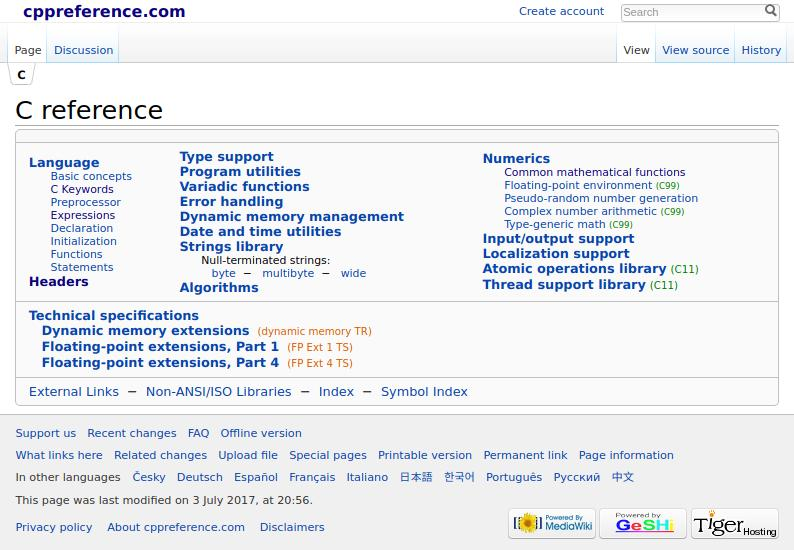
\includegraphics[width=\linewidth]{./gfx/cpp-home}
	\caption{Die Startseite der C-Referenz \url{https://en.cppreference.com/w/c}} \label{fig:cpp-home}
\end{figure}

Der angegebene Link führt Sie auf die \emph{englische} Befehlsreferenz. Übersetzungen in verschiedene andere Sprachen, darunter auch Deutsch, stehen zur Verfügung. In der Regel sind diese aber weit weniger ausführlich und oft unvollständig\footnote{Meiner Erfahrung nach gilt dies generell in der Welt des Programmierens: Nützliche Ressourcen sind oft nur in Englisch verfügbar oder nur in dieser Sprache in vollem Umfang.}. Wenn Sie dennoch mit der deutschen Version arbeiten möchten, finden Sie auf jeder Seite der Referenz am unteren Rand die Zeile \emph{In other languages} und dahinter Links, die sie zu einer entsprechenden Übersetzung führen.

Am rechten oberen Rand befindet sich eine Textbox, in die Sie einen Suchbegriff eingeben können. Die Suche liefert ihnen Ergebnisse zu ihrem Begriff sowie zu \enquote{ähnlichen Ausdrücken}. Die Ergebnisse sind in zwei Spalten sortiert und betreffen die Sprache C++ (links) bzw. C (rechts). In Abbildung \ref{fig:cpp-search} finden Sie das Ergebnis der Suche nach dem Befehl \texttt{printf}. Jede Zeile der Suchergebnisse ist ein Link auf einen Artikel, der den Befehl oder das Konzept erklärt.

\begin{figure}[h!]
	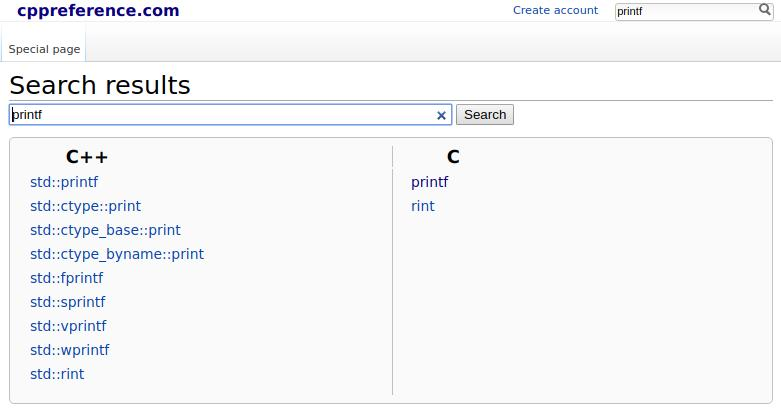
\includegraphics[width=\linewidth]{./gfx/cpp-search}
	\caption{Suchergebnisse in der CPP-Referenz} \label{fig:cpp-search}
\end{figure}

Ein solcher Artikel sieht \idR aus wie in Abbildung \ref{fig:cpp-printf}. Befehle, die sich sehr ähnlich verhalten werden teils zu einem einzelnen Artikel zusammengefasst. Nach der Überschrift finden Sie die Zeile \emph{Defined in header <stdio.h>}, die Ihnen mitteilt, welche \mintinline{c}{#include}s Sie setzen müssen, um den oder die erklärten Befehle in Ihren Programmen nutzen zu können.

Weiter schließt sich eine Syntax-Übersicht an, in der die erwarteten Parameter sowie ihre Datentypen aufgelistet werden. Manche dieser Formen standen nicht in der \enquote{Urform} der Sprache C zur Verfügung. Für solche Features, die erst mit einem bestimmten Standard eingeführt wurden ist in der Referenz in grün das Einführungsdatum bzw. das \enquote{Verfallsdatum} der Form aufgeführt. Ich erinnere Sie daran, dass wir hier den Standard C11 besprechen. In Abschnitt \ref{sec:cpp-article} werden wir anhand eines übersichtlicheren Beispiels auf die Struktur der Artikel eingehen.

\begin{figure}[h!]
	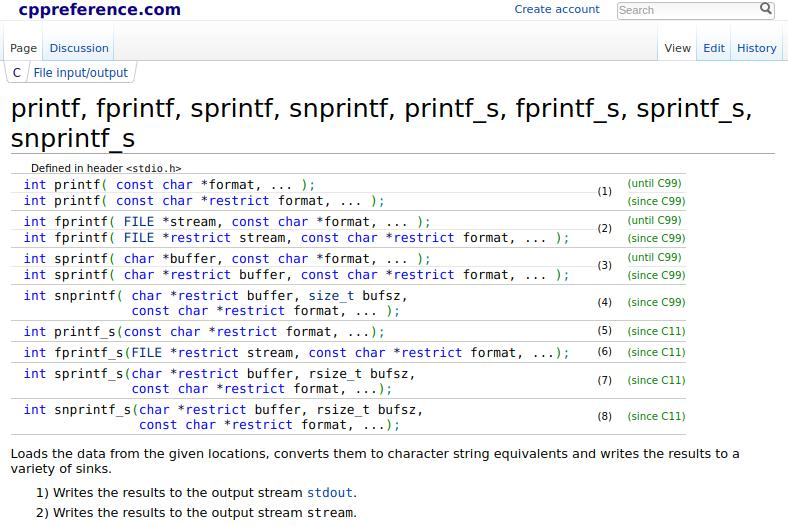
\includegraphics[width=\linewidth]{./gfx/cpp-printf}
	\caption{Anfang des Artikels zu \texttt{printf} auf der CPP-Referenz} \label{fig:cpp-printf}
\end{figure}

\section{Funktionen zu einer Aufgabe finden}
Die Funktionen, die die Sprache C zur Verfügung stellt, sind in thematisch verwandten \emph{Bibliotheken} organisiert. Zu jeder Bibliothek existiert ein \emph{Header}, dessen Name einen Hinweis auf die darin enthaltenen Funktionen gibt. Um Lösungen zu einem gegebenen Problem zu suchen, durchsucht man also am besten die Liste der Header. Diese kann von der Hauptseite aus über den Link \emph{Headers} erreicht werden (siehe Abbildung \ref{fig:cpp-home}, erste Spalte unten). Dieser Link führt Sie zu einer Ansicht wie in Abbildung \ref{fig:cpp-headers}.

\begin{figure}[h!]
	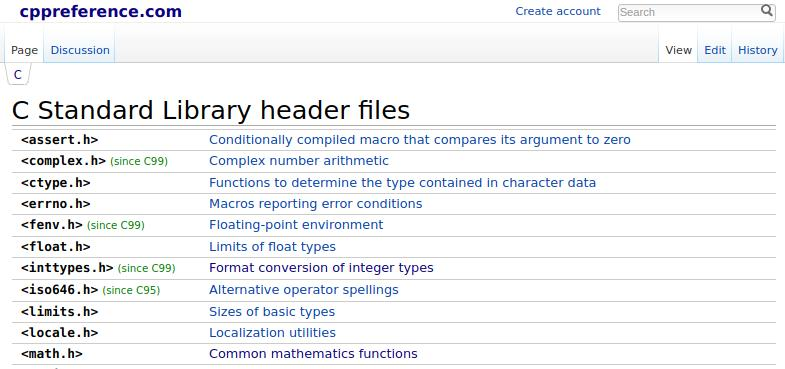
\includegraphics[width=\linewidth]{./gfx/cpp-headers}
	\caption{Liste der Header auf der CPP-Referenz} \label{fig:cpp-headers}
\end{figure}

In diesem Kapitel wollen wir uns mit mathematischen Funktionen befassen; wir klicken daher auf den Link \emph{Common mathematical functions}.

\begin{figure}[h!]
	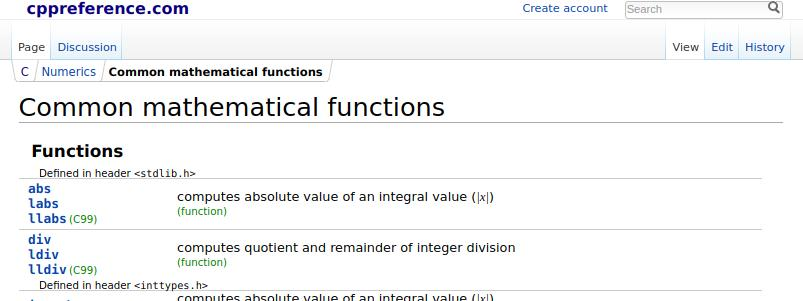
\includegraphics[width=\linewidth]{./gfx/cpp-math}
	\caption{Funktionen der math-library in der CPP-Referenz} \label{fig:cpp-math}
\end{figure}

Wie Sie in Abbildung \ref{fig:cpp-math} sehen, sind die Funktionen in einem ähnlichen Format aufgelistet wie schon die Header. Zu vielen Aufgaben stehen mehrere Funktionen zur Verfügung. Dies hat den Grund, dass die Sprache C \emph{strong-typed} ist, \ie dass Unterschiede zwischen beispielsweise \mintinline{c}{float}- und \mintinline{c}{double}-Werten bestehen. Funktionen, die mit einem \texttt{f} beginnen, berechnen \idR einen \mintinline{c}{float}-Wert; der Anfang \texttt{l} weist auf einen \mintinline{c}{long}-Wert hin und \texttt{ll} erzeugt einen \mintinline{c}{long long}-Wert. Für manche Kontexte sind Ganzzahlen unsinnig; dort weist der Suffix \texttt{l} auf \mintinline{c}{long double} hin. Ist dem Funktionsnamen kein solcher \emph{Präfix} vorangestellt, wird ein \mintinline{c}{double}-Wert berechnet\footnote{Die Benennungs-Logik der C-Standardbibliotheken folgt oft noch veralteten Konventionen, die solche kryptischen Namen hervorbringen. Moderne ProgrammiererInnen bevorzugen \enquote{klare Namen}. Damit auch ältere Code-Teile weiterhin funktionieren musste diese Benennungsregeln fortgeführt werden.}.

Aufgrund des \emph{strong typing} muss auch für die Argumente der Funktionen unterschieden werden. Hier geben die \emph{Suffixe} \texttt{f}, \texttt{l} und \texttt{ll} den Datentyp des Arguments an.

Beispielsweise finden Sie die Funktion \texttt{abs}, die den Absolutbetrag einer \mintinline{c}{double}-Zahl berechnet und als \mintinline{c}{double}-Wert zurückgibt. Daneben ist aber auch \ua die Funktion \texttt{fabsl} aufgelistet, die ebenso den Absolutbetrag einer Zahl berechnet. Die Zahl wird für diese Funktion jedoch als \mintinline{c}{long}-Wert angegeben und das Ergebnis als \mintinline{c}{float} berechnet.

\section{Der Artikel zu \texttt{sqrt}} \label{sec:cpp-article}
\begin{figure}[h!]
	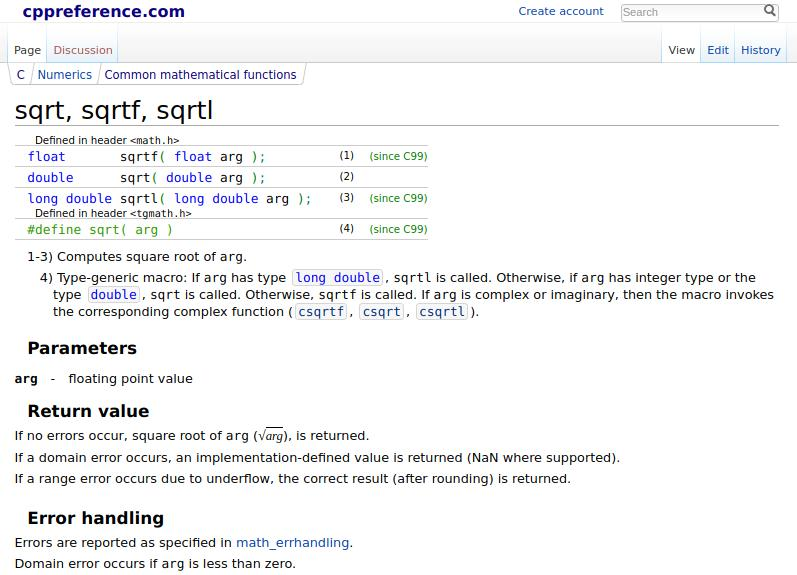
\includegraphics[width=\linewidth]{./gfx/cpp-sqrt}
	\caption{Anfang des Artikels zu \texttt{sqrt} in der CPP-Referenz} \label{fig:cpp-sqrt}
\end{figure}

Abbildung \ref{fig:cpp-sqrt} zeigt den Anfang des Artikels zum Befehl \texttt{sqrt}. Die Zeile \emph{Defined in header <math.h>} weist darauf hin, dass wir \mintinline{c}{#include <math.h>} setzen müssen, um \texttt{sqrt} benutzen zu können. Von dem Befehl stehen drei Varianten zur Verfügung, von denen zwei erst mit dem Standard C99 eingeführt wurden (Punkte 1 bis 3). Weiterhin wurde mit dem Standard C99 ein \emph{Makro} eingeführt (Punkt 4), das wir an dieser Stelle noch nicht bearbeiten wollen. In Kapitel \ref{chp:Preprocessor} besprechen wir die hierzu relevanten Techniken. Für den Moment können Sie den Punkt ignorieren\footnote{Wenn Sie später im Kursverlauf nochmals diesen Artikel in der Referenz lesen, beachten Sie bitte, dass für die Benutzung des Makros der Header \emph{<tgmath.h>} eingebunden werden muss.}.

Unter der tabellarischen Übersicht der im Artikel besprochenen Funktionen finden Sie eine Kurzbeschreibung des Effekts der einzelnen Formen. \emph{1-3) Computes square root of arg.} -- alle hier besprochenen Funktionen berechnen also die Quadratwurzel eines Arguments \texttt{arg}. Der Unterschied ist der Datentyp des Ergebnisses bzw. des Arguments.

Unter \emph{Parameters} finden Sie genauere Erläuterungen zu den Argumenten, die den Funktionen übergeben werden können. Für \texttt{sqrt} ist dies die nüchterne Erklärung, dass \texttt{arg} eine beliebige Fließkommazahl beschreibt. Bei der Funktion \texttt{printf} wird hier etwa aufgelistet, wie ein Formatstring auszusehen hat.

Funktionen berechnen einen Wert, der dann einer anderen Variablen zugewiesen werden kann. Betrachten Sie das folgende Beispiel:

\begin{codebox}[Beispiel: Betrag einer Zahl  mit dem ternären Operator]
\begin{minted}[linenos]{c}
#include <math.h>

int main () {
   double root = sqrt(81.0);
}
\end{minted}
\end{codebox}

Wir benutzen die Funktion \texttt{sqrt} um aus dem \mintinline{c}{double}-Wert \texttt{81.0} die Wurzel zu berechnen und speichern diesen Wert der Wurzel dann in der Variablen \texttt{root}. Dieser berechnete Wert wird als Rückgabewert (\emph{Return Value}) der Funktion bezeichnet.

Der Abschnitt \emph{Return Values} gibt Details zu dem berechneten Wert unter der Annahme verschiedener Szenarios.

Wenn kein Fehler auftritt, wird die Quadratwurzel von \texttt{arg} berechnet. Wie Sie wissen, existiert aber nicht zu jeder Zahl eine Quadratwurzel. So sind negative Werte für \texttt{arg} nicht zulässig -- dies ist gemeint mit \emph{If a domain error occurs}. In diesem Fall hängt das Ergebnis von der Version des Compilers ab (\emph{an implementation-defined value is returned}). In der Regel wird aber ein spezielles Bitmuster erzeugt, das sicher als \enquote{Fehler-Wert} interpretiert werden kann (\emph{NaN where supported} -- \emph{NaN} steht für \emph{Not a Number}, also ein Fehlerwert. Siehe hierzu mehr in Abschnitt \ref{sec:NAN}).

Die letzte Zeile \emph{If a range error occurs due to underflow} beschreibt das Verhalten, wenn der Wert von \texttt{arg} nicht mehr korrekt mit seinem Datentyp abgebildet werden kann (vgl. Abschnitt \ref{sec:Datatypes} im Anhang -- manche Werte sind zu groß oder haben zu viele Nachkommastellen, um beispielsweise als \mintinline{c}{double} exakt abgebildet zu werden). In diesem Fall wird mit einem gerundeten Wert gerechnet.

Unter \emph{Error Handling} werden weitere Details aufgelistet, die das Verhalten von \texttt{sqrt} in \enquote{abnormalen} Situationen beschreiben. Im Allgemeinen ist es nicht nötig, all diese Details im Kopf zu behalten -- dafür ist die Referenz da.

Am Ende der meisten Artikel finden Sie zu jedem Befehl einen Beispiel-Code, der die Anwendung der besprochenen Funktion verdeutlicht, sowie ein Ausgabebeispiel.

\section{Weitere nützliche Funktionen der math-library}
Die folgende Tabelle listet sehr gebräuchliche Funktionen sowie eine Kurzbeschreibung auf. Mit der cpp-Referenz sollten Sie nun dazu in der Lage sein, diese Funktionen in Ihren Programmen anzuwenden.

\begin{table}[h!]
	\newcolumntype{C}{>{\ttfamily\centering\arraybackslash} p{.2\linewidth}}
	\newcolumntype{D}{>{         \centering\arraybackslash} p{.7\linewidth}}
	\rowcolors{1}{white}{chameleonblue2}
\begin{center}
\begin{tabularx}
	{.95\linewidth}
	{CD}
\toprule[1pt]

	\normalfont Funktion  &  Effekt
\tabcrlf

	sqrt  & Quadratwurzel einer Zahl \\
	cbrt  & Kubikwurzel einer Zahl   \\
	pow   & Potenz einer Zahl \texttt{x} zu einem Exponenten \texttt{y}: $x^{y}$ \\
	exp   & Exponentialfunktion      \\
	log   & Natürlicher Logarithmus  \\
	sin   & Sinus                    \\
	cos   & Cosinus                  \\
	tan   & Tangens                  \\
	asin  & Arcussinus               \\
	acos  & Arcuscosinus             \\
	atan  & Arcustangens             \\
	atan2 & Arcustangens mit Unterscheidung der Quadranten \\
	ceil  & Zahl aufrunden           \\
	floor & Zahl abrunden            \\
	trunc & Nachkommaanteil abschneiden \\
	round & Zahl runden              \\

\bottomrule[1pt]
\end{tabularx}
\end{center}
\caption{Gängige Funktionen der math-library}\label{tab:CommonMathFuncs}
\end{table}

\section{Die C++-Referenz}
\begin{plusbox}
Wie die URL der Seite schon vermuten lässt, ist die cpp-Referenz auch ein Verzeichnis der Features von C++. Gehen Sie hierzu von der Adressse \url{https://en.cppreference.com/w/cpp} aus, um Informationen spezifisch zu C++ zu finden.

Sie haben bereits gesehen, dass die Stichwortsuche direkt auf C++-spezifische Artikel verweist. Auf der Startseite der C++-Referenz finden Sie ebenfalls den Punkt \emph{Headers}, von wo Sie auf die spezifischen libraries verwiesen werden. Die bedeutsamsten Bibliotheken sind hier aber schon direkt von der Startseite aus verlinkt.
\end{plusbox}

	\chapter{Schleifen} \label{chp:loops}
\epigraph{You spin me right round, baby // Right round like a record, baby // Right round round round}
{Dead Or Alive}

Computer können dazu benutzt werden, die immer gleichen (lästigen) Aufgaben wiederholt und in schneller Folge auszuführen. Es ist möglich, bei jeder Wiederholung einen einzelnen Eingabewert zu ändern und so \eg Berechnungen für einen ganzen Wertebereich durchzuführen, oder Messwerte von einem Gerät zu überwachen.

Zeichnet man ein \emph{Flussdiagramm} eines solchen Programms (wie in Abbildung \ref{fig:FlowBasicLoop}), so findet sich in der Regel ein Programmteil, der zur Vorbereitung dient und in gewohnter Weise \enquote{von oben nach unten} abgearbeitet wird. An diesen schließt sich ein Abschnitt an, der einige Male wiederholt werden soll, und daher im Flussdiagramm als Bogen dargestellt wird. Nach diesem Teil könnte die Ausgabe der Ergebnisse stattfinden, die wiederum in gewohnter \emph{linearer} Weise (also von oben nach unten) bearbeitet wird. 

Die Form dieses Flussdiagramms motiviert den Namen \emph{Schleife} für eine solche Struktur.

\begin{figure}[h!]
\begin{center}
\begin{tikzpicture}
    \node at (0, 3  ) (Input)      {Vorbereitung};
    \node at (0, 1.5) (Operations) {Wiederholungen};
    \node at (0, 0  ) (Output)     {Nachbereitung};
    
    \draw [->] (Input) -- (Operations);
    \draw [->] (Operations.south)arc(-160:160:1.0);		%start angle: stop angle : radius
    \draw [->] (Operations) -- (Output);
\end{tikzpicture}
\caption{Programmflussdiagramm mit Schleife} \label{fig:FlowBasicLoop}
\end{center}
\end{figure}

In der Regel ist die Zahl der Schleifendurchläufe an eine Bedingung geknüpft; genauso sind aber auch \emph{Endlosschleifen} möglich. In diesem Kapitel werden wir verschiedene Schleifentypen und ihre Anwendungsfelder kennen lernen.

\begin{hintbox}[Laufende Programme zum Beenden zwingen: \texttt{STRG + C}]
Macht man einen Fehler bei der Formulierung der Bedingung, so kann man unbeabsichtigt eine Endlosschleife erstellen. Ein solches Programm wird von sich selbst aus nie beendet. Wir können zu jeder Zeit aber das Beenden erzwingen, indem wir in der Konsole die Tastenkombination \texttt{STRG + C} drücken.
\end{hintbox}

\section{Programmsprünge: \mintinline{c}{goto}}
Die einfachste Form, Schleifen zu implementieren, funktioniert über die \emph{Sprunganweisung} \mintinline{c}{goto}. Stellen wir uns vor, der Computer würde mit einem Cursor durch unser Programm laufen und Zeile für Zeile bearbeiten, so ist \mintinline{c}{goto} der Befehl, den Cursor an eine bestimmte Stelle zu verschieben. Sprünge sind sowohl vorwärts als auch rückwärts möglich.

Für einen Sprung ist zunächst eine \emph{Sprungmarke} nötig, also ein Punkt, ab der das Programm fortgeführt wird. Eine solche Sprungmarke hat einen Namen, der denselben Regeln folgt, wie Variablennamen (darf nur einmal im Programm vorkommen; Unterscheidung von Groß- und Kleinschreibung; nur alphanumerische Zeichen; darf nicht mit einer Zahl beginnen; maximal 40 Zeichen lang). Im Code wird sie durch einen Doppelpunkt abgeschlossen.

Der Sprung selbst folgt dann der Syntax:
\begin{codebox}[Syntax: \texttt{goto}]
\begin{minted}{c}
goto Sprungmarke;
\end{minted}
\end{codebox}

Hier sehen Sie ein einfaches Anwendungsbeispiel:
\begin{codebox}[Beispiel: Sprünge mit \texttt{goto}]
\begin{minted}[linenos]{c}
#include <stdio.h>

int main () {
   printf("Erste Zeile der Ausgabe.\n");
   goto ReEntryPoint;   
   
   printf("Dies wird nie ausgegeben.\n");
   
   ReEntryPoint:
   printf("Letzte Zeile der Ausgabe.\n");
}
\end{minted}
\end{codebox}

Nach der Ausgabe in Zeile 4 springt der \enquote{Cursor} weiter zu Zeile 9. Aller Code dazwischen wird nie ausgeführt. Die Ausgabe lautet entsprechend:

\begin{cmdbox}[Ausführungsbeispiel: Sprünge mit \texttt{goto}]
\begin{minted}{text}
Erste Zeile der Ausgabe.
Letzte Zeile der Ausgabe.
\end{minted}
\end{cmdbox}

Wir können Sprünge mit Sprünge mit \mintinline{c}{if} an eine Bedingung knüpfen und so eine Schleife erzeugen, die auch wieder verlassen wird:

\begin{codebox}[Beispiel: Quadratwurzeln der Zahlen 1 bis 10 mit \texttt{goto}]
\begin{minted}[linenos]{c}
#include <stdio.h>
#include <math.h>

int main () {
   double foo = 1;
\end{minted}
\end{codebox}
%
\begin{codebox}[]
\begin{minted}[linenos, firstnumber=last]{c}
   iterationPoint:
   printf("Die Wurzel aus %4.1lf ist %lf.\n", foo, sqrt(foo));
   foo++;
   
   if (foo <= 10) {goto iterationPoint;}
   
   printf("Erfolgreicher Programmabschluss.\n");
}
\end{minted}
\end{codebox}

\begin{cmdbox}[Ausführungsbeispiel: Quadratwurzeln der Zahlen 1 bis 10 mit \texttt{goto}]
\begin{minted}{text}
Die Wurzel aus  1.0 ist 1.000000.
Die Wurzel aus  2.0 ist 1.414214.
Die Wurzel aus  3.0 ist 1.732051.
Die Wurzel aus  4.0 ist 2.000000.
Die Wurzel aus  5.0 ist 2.236068.
Die Wurzel aus  6.0 ist 2.449490.
Die Wurzel aus  7.0 ist 2.645751.
Die Wurzel aus  8.0 ist 2.828427.
Die Wurzel aus  9.0 ist 3.000000.
Die Wurzel aus 10.0 ist 3.162278.
Erfolgreicher Programmabschluss.
\end{minted}
\end{cmdbox}

\begin{warnbox}[Spaghetti-Code]
Was Sie gerade über \mintinline{c}{goto} gehört haben, dient vor allem dem besseren Verständnis der folgenden Schleifentypen. Programme, die viele \mintinline{c}{goto}-Sprunganweisungen enthalten werden schnell unübersichtlich. Die einzelnen \enquote{Fäden} des Programmes kreuzen sich und laufen durcheinander wie Spaghetti auf einem Teller. Es wird schwierig, den Programmfluss zu verfolgen und Fehler sammeln sich an.

Die folgenden Schleifentypen sind für Menschen besser zu bedienen, werden aber vom Compiler ebenso in \mintinline{c}{goto}-Programmsprünge umgesetzt.

Es ist prinzipiell immer möglich, ohne den Befehl \mintinline{c}{goto} auszukommen und in den weit meisten Fällen auch zu bevorzugen. ProgrammiererInnen diskutieren kontrovers, ob der Befehl aus dem Sprachumfang der Sprache C (oder damit verwandten Sprachen) gestrichen werden sollte. In Abschnitt \ref{sec:ControlFluxAdjustment} werden Sie allerdings einen Fall sehen, wo \mintinline{c}{goto} tatsächlich eine \emph{elegantere} Lösung darstellt, als die Alternativen.
\end{warnbox}

\section{Schleife mit Bedingung: \mintinline{c}{while}}
Das Schlüsselwort \mintinline{c}{while} lehnt sich an den Sprachgebrauch an, und implementiert die Idee: WÄHREND \emph{Bedingung erfüllt} WIEDERHOLE \emph{Anweisungen}. Dabei ist \emph{Bedingung} ein Ausdruck wie schon bei \mintinline{c}{if}, der zu einem Wahrheitswert ausgewertet werden kann. Die Syntax lautet:

\begin{codebox}[Syntax: \texttt{while}]
\begin{minted}{c}
while (Bedingung) {
   Anweisungen;
}
\end{minted}
\end{codebox}

Mit diesem Schlüsselwort übersetzt sich also das vorige Beispiel zu folgendem Code:

\begin{codebox}[Beispiel: Quadratwurzeln der Zahlen 1 bis 10 mit \texttt{while}]
\begin{minted}[linenos]{c}
#include <stdio.h>
#include <math.h>

int main () {
   double foo = 1;
   
   while (foo <= 10) {
      printf("Die Wurzel aus %4.1lf ist %lf.\n", foo, sqrt(foo));
      foo++;
   }
   
   printf("Erfolgreicher Programmabschluss.\n");
}
\end{minted}
\end{codebox}

Wie schon bei \mintinline{c}{if} können bei einzeiligen Anweisungsblocks die \{geschweiften Klammern\} entfallen. Aus denselben Gründen wie dort empfehle ich aber, immer Klammern zu setzen.

Die Bedingung wird bereits vor Eintritt in die Schleife überprüft. Ist sie vor dem Eintritt nicht erfüllt, wird der Schleifen-Körper nie ausgeführt sondern komplett übersprungen.

\begin{hintbox}[Absichtliche Endlosschleife]
Es gibt Situationen, in denen eine Schleife bewusst endlos lange laufen soll, \eg um ein Gerät zu überwachen, das nie abgeschalten wird, oder weil andere Mechanismen das Verlassen der Schleife bewirken können. Für diesen Fall setzt man für gewöhnlich einfach
\begin{center}
\mintinline{c}{while (1)}
\end{center}
Die Konstante \texttt{1} kann sich nicht ändern und entspricht direkt dem Wahrheitswert \emph{true}.
\end{hintbox}

\section{Schleife mit Bedingung und einem garantierten Durchlauf: \mintinline{c}{do-while}}
Schleifen mit dem Konstrukt \mintinline{c}{do-while} funktionieren nach demselben Prinzip wie \mintinline{c}{while}-Schleifen. Allerdings findet die Prüfung der Bedingung erst \emph{am Ende der Schleife} statt, und nicht schon vor Eintritt in die Schleife. Dies bewirkt, dass der Schleifenkörper mindestens einmal durchlaufen wird.

Die Syntax ist sehr ähnlich der von \mintinline{c}{while}:
\begin{codebox}[Syntax: \texttt{do-while}]
\begin{minted}{c}
do {
   Anweisungen;
} while (Bedingung);
\end{minted}
\end{codebox}

Die folgenden beiden Beispiele und Ausgaben verdeutlichen den Unterschied:
\begin{tcbraster}[raster columns=2,
                  raster equal height,
                  nobeforeafter,
                  raster column skip=0.5cm]
\begin{codebox}[Schleife mit \texttt{while}]
\begin{minted}[linenos]{c}
#include <stdio.h>

int main () {
   unsigned int foo = 0;
   
   while (foo > 0) {
      printf("Schleifenkörper.\n");
   }
   
   printf("Programmende.\n");
}
\end{minted}
\end{codebox}
%
\begin{codebox}[Schleife mit \texttt{do-while}]
\begin{minted}[linenos]{c}

#include <stdio.h>

int main () {
   unsigned int foo = 0;
   
   do {
      printf("Schleifenkörper.\n");
   } while (foo > 0);
   
   printf("Programmende.\n");
}
\end{minted}
\end{codebox}
\end{tcbraster}

In beiden Fällen ist die Bedingung \texttt{foo > 0} zu keiner Zeit erfüllt. Dennoch sind die beiden Ausgaben unterschiedlich:

\begin{tcbraster}[raster columns=2,
                  raster equal height,
                  nobeforeafter,
                  raster column skip=0.5cm]
\begin{cmdbox}[Ausführungsbeispiel: Schleife mit \texttt{while}]
\begin{minted}{text}
Programmende.
\end{minted}
\end{cmdbox}
%
\begin{cmdbox}[Ausführungsbeispiel: Schleife mit do-while]
\begin{minted}{text}
Schleifenkörper.
Programmende.
\end{minted}
\end{cmdbox}
\end{tcbraster}

\section{Zählschleifen: \mintinline{c}{for}}
Der Schleifen-Typ \mintinline{c}{while} ist generell für alle Szenarios geeignet. Das häufigste Szenario ist der Fall, in dem eine Variable für jede \emph{Iteration} (\ie für jeden Durchlauf der Schleife) hochgezählt wird. Zu diesem Zweck existiert die spezielle Form der \mintinline{c}{for}-Schleife, die eine kompakte Form solcher Konstrukte erlaubt.

Eine \mintinline{c}{for}-Schleife hat die folgende Form:
\begin{codebox}[Syntax: \texttt{for}]
\begin{minted}{c}
for (Startanweisung; Bedingung; Iteration) {
   Anweisungen;
}
\end{minted}
\end{codebox}

Wobei \texttt{Startanweisung} und \texttt{Iteration} jeweils reguläre C-Anweisungen sind und \texttt{Bedingung} ein Ausdruck, der zu einem Wahrheitswert ausgewertet werden kann. Diese Struktur wird genauso umgesetzt, als würde eine \mintinline{c}{while}-Schleife folgender Form programmiert:

\begin{codebox}[Äquivalente Form mit \texttt{while}]
\begin{minted}{c}
Startanweisung;
while (Bedingung) {
   Anweisungen;
   Iteration;
}
\end{minted}
\end{codebox}

Das heißt, \texttt{Startanweisung} wird automatisch vor Schleifenbeginn und \texttt{Iteration} am Ende jedes Schleifendurchlaufs ausgeführt. In der Regel ist \texttt{Startanweisung} die Zuweisung eines Startwerts zu einer \emph{Zählvariablen}. Mit \texttt{Iteration} wird diese Zählvariable dann hochgezählt (oder in geeigneten Schritten verändert).

Das vorige Beispiel der Quadratwurzeln bis 10 schreibt sich damit folgendermaßen:

\begin{codebox}[Beispiel: Quadratwurzeln der Zahlen 1 bis 10 mit \texttt{for}]
\begin{minted}[linenos]{c}
#include <stdio.h>
#include <math.h>

int main () {
   double foo;
   
   for (foo = 1; foo <= 10; foo++) {
      printf("Die Wurzel aus %4.1lf ist %lf.\n", foo, sqrt(foo));
   }
   
   printf("Erfolgreicher Programmabschluss.\n");
}
\end{minted}
\end{codebox}

Mit dem Standard C99 wurde auch die Möglichkeit eingeführt, in \emph{Startanweisung} Variablen zu deklarieren. Diese \enquote{existieren} dann allerdings nur innerhalb des Schleifenkörpers und können nach Ende der Schleife nicht mehr verwendet werden. (Es dürfen jedoch nach der Schleife \emph{neue} Variablen mit demselben Namen angelegt werden.) Wir werden in Abschnitt \ref{sec:Scopes} mehr hierzu erfahren. Das folgende Beispiel zeigt diese kombinierte Deklaration und Initialisierung:

\begin{codebox}[Beispiel: \texttt{for}-Schleife mit Deklaration]
\begin{minted}[linenos]{c}
#include <stdio.h>
#include <math.h>

int main () {
   for (double foo = 1; foo <= 10; foo++) {
      printf("Die Wurzel aus %4.1lf ist %lf.\n", foo, sqrt(foo));
   }
   
   printf("Erfolgreicher Programmabschluss.\n");
}
\end{minted}
\end{codebox}

\section{Eingriffe in den Kontrollfluss: \mintinline{c}{break} und \mintinline{c}{continue}} \label{sec:ControlFluxAdjustment}
Es gibt Situationen, in denen eine Schleifen-Ausführung \enquote{vorzeitig} abgebrochen oder ein Teil des Schleifenkörpers \enquote{übersprungen} werden soll. Zu diesem Zweck dienen die Befehle \mintinline{c}{break} und \mintinline{c}{continue}.

Wir kennen \mintinline{c}{break} bereits von \mintinline{c}{switch}-Blöcken. Dort wurden sie benutzt, um den aktuellen \mintinline{c}{switch}-Block zu verlassen und mit der Programmausführung an das Ende des Blocks zu springen. Eben dieselbe Wirkung hat \mintinline{c}{break} auch bei Schleifen, gleich ob es sich dabei um \mintinline{c}{for}, \mintinline{c}{while} oder \mintinline{c}{do-while} handelt.

Das folgende Beispiel verwendet \mintinline{c}{break}, um Zahlen und ihre Quadrate auszugeben. Dabei sollen maximal 100 Zahlen ausgegeben werden, und die Ausgabe soll stoppen, wenn eine Quadratzahl größer als 1000 ist\footnote{Natürlich kann dazu auch ein logisches OR benutzt werden; hier soll aber die Anwendung von \mintinline{c}{break} illustriert werden.}.

\begin{codebox}[Beispiel: Abbruch einer \texttt{for}-Schleife mit \texttt{break}]
\begin{minted}[linenos]{c}
#include <stdio.h>

int main () {
   for (int foo = 1; foo <= 100; foo++) {
      printf("%d -> %d.\n", foo, foo * foo);
      if (foo * foo > 1000) {break;}
   }
}
\end{minted}
\end{codebox}

Die Zahlen 1 bis 32 sowie ihre Quadrate (1 bis 1024) werden ausgegeben, bevor die Schleife durch  \mintinline{c}{break} verlassen wird und die Ausgabe stoppt.

\mintinline{c}{continue} greift ähnlich in die Ausführung ein; jedoch wird die Schleife nicht verlassen sondern die Ausführung springt zum Schleifenbeginn zurück. Bei \mintinline{c}{for}-Schleifen wird zuvor noch \texttt{Iteration} ausgeführt, \ie \eg die Zahlvariable hochgezählt.

Das folgende Beispiel gibt die Zahlen von 1 bis 100 aus mit Ausnahme der durch 5 teilbaren Zahlen:

\begin{codebox}[Beispiel: \texttt{for} mit \texttt{continue}]
\begin{minted}[linenos]{c}
#include <stdio.h>

int main () {
   for (int foo = 1; foo <= 100; foo++) {
      if (foo % 5 == 0) {continue;}
      printf("%d\n", foo);
   }
}
\end{minted}
\end{codebox}
	\chapter{Arrays und dynamische Programmierung}
\epigraph{If debugging is the process of removing software bugs, then programming must be the process of putting them in.}
{Edsger Dijkstra}

Bis hierhin haben wir sehr kleine Datenmengen behandelt. Unser bisheriges \enquote{Arbeitsmaterial} waren Variablen, die einige wenige Bytes halten. Eine Stärke von Computern ist es aber gerade, große Datenmengen schnell zu verarbeiten. Hier werden wir Möglichkeiten kenenn lernen, nahezu beliebig große Datenmengen im Speicher zu halten und zu manipulieren.

\section{Arrays} \label{sec:Arrays}
\emph{Arrays} (Felder) sind Gruppen von Variablen, die man sich als nummerierte Liste vorstellen kann. Die einzelnen Elemente werden über ihren \emph{Index} angesprochen, also die \enquote{Nummer der Zeile in der Liste}. Die Nummerierung beginnt hierbei \emph{bei der 0}. Alle Elemente eines Arrays haben denselben Datentyp; man sagt daher auch, das Array selbst habe einen bestimmten Datentyp.

Das Handling von Arrays geschieht über Pointer. Man speichert die Adresse des ersten Elements. Im Speicher liegen alle Werte dicht an dicht hintereinander. Um etwa das dritte Element eines Arrays anzusprechen (zu lesen oder zu überschreiben) geht man von der \emph{Startadresse} um zwei Schritte weiter. Der Abstand zur Start-Adresse wird auch \emph{Offset} genannt. Bei Arrays, deren Elemente nur ein einzelnes Byte groß sind sind also Offset und Index gleich.

\begin{tcolorbox}[title=Speicherbild]
\begin{center}
\begin{tikzpicture}
  [ 
    cell/.style={text width=8mm,
    text height=4mm, draw=black, inner sep=1mm},
    ld/.style={draw=blue,shorten >=2pt,->}
  ]
  \node (c1) at (0,0) [cell] {\ttfamily 99};
  \node (c2) at (1,0) [cell] {\ttfamily 1};
  \node (c3) at (2,0) [cell] {\ttfamily 255};
  \node (c4) at (3,0) [cell] {\ttfamily 0};
  \node (c5) at (4,0) [cell] {\ttfamily 80};
  \node (c6) at (5,0) [cell] {\ttfamily ...};

  \node (labelMem) at (7,  0) {Speicher};
  \node (labelMem) at (7,  1) {Indizes};
  \node (labelMem) at (7, -1) {Adressen};
  
  \node (a1) [below=2mm of c1]            {\tiny 0x27ff};
  \node (a2) [below=2mm of c2, color=red] {\tiny 0x2800};
  \node (a3) [below=2mm of c3]            {\tiny 0x2801};
  \node (a4) [below=2mm of c4]            {\tiny 0x2802};
  \node (a5) [below=2mm of c5]            {\tiny 0x2803};
  \node (a6) [below=2mm of c6]            {\tiny 0x2804};
  
  \node (ptr) [below=8mm of c1] {\scriptsize\ttfamily Startadresse};
  \node (vc2) [above=6mm of c1] {\scriptsize\ttfamily Index 2};
  \node (vc0) [above=2mm of c1] {\scriptsize\ttfamily Index 0};
  
  \draw [ld] (ptr.east) .. controls +(0.3,0) .. (a2.south);
  \draw [ld] (vc0.east) .. controls +(0.4,0) .. (c2.north);
  \draw [ld] (vc2.east) .. controls +(2.4,0) .. (c4.north);
\end{tikzpicture}
\end{center}
\end{tcolorbox}

\subsection{Syntax-Elemente}
Wie alle Variablen müssen auch Arrays zuerst deklariert werden. Dies geschieht in der Form:

\begin{codebox}[Syntax: Arrays deklarieren]
\begin{minted}{c}
Datentyp Name[ElementAnzahl];
\end{minted}
\end{codebox}

Damit wird ein Array vom Typ \texttt{Datentyp} angelegt, das \emph{ElementAnzahl} Elemente hat und über die Variable \texttt{Name} angesprochen werden kann. Achtung: Die Variable \texttt{Name} selbst ist vom Typ \texttt{Datentyp *}, also ein \emph{Pointer auf Daten vom Typ \texttt{Datentyp}}. Man nennt die einzelnen Elemente eines Arrays auch \emph{Instanzen von \texttt{Datentyp}}.

Wir greifen (sowohl lesend als auch schreibend) auf Arrays zu, indem wir in [eckingen Klammern] den Index des Elements schreiben, das wir ansprechen möchten (\ie seine \enquote{Nummer} in einer Liste). Man spricht von \emph{indiziertem Array-Zugriff}.

\begin{warnbox}[Indizierung ab 0]
Achtung: Indizes beginnen bei \texttt{0}. Das bedeutet, dass das letzte gültige Element des Arrays den Index \texttt{ElementAnzahl - 1} hat. Der Compiler führt bei Array-Zugriffen keine Gültigkeitskontrolle der Indizes durch. Es ist also möglich, ein Array mit 10 Elementen zu deklarieren, dann aber auf das 11. Element zuzugreifen. Wie schon in in Kapitel \ref{chp:Input} erklärt wurde, erzeugt Lese- und Schreibzugriff auf \emph{nicht-reservierte Speicherbereiche} undefiniertes Verhalten; mögliche Effekte sind Überschreiben von anderen Variablen, Programmabsturz, aber auch \enquote{nichts}, abhängig von der Struktur des Programmes. Auch, wenn ein fehlerhafter Arrayzugriff zunächst keinen Effekt hat, sollten Sie solche Speicherzugriffe dringend vermeiden, da sonst spätere Erweiterungen am Programm nicht mehr funktionieren können, obwohl diese korrekt programmiert sind.

Achten Sie daher genau auf die Codeteile, die Ihre Array-Zugriffe bestimmen.
\end{warnbox}

\begin{codebox}[Beispiel: Array-Zugriffe]
\begin{minted}[linenos]{c}
#include <stdio.h>

int main () {
   int list[100];
   
   list[42] = 666;
   
   printf("Das 43. Element der Liste 'list' ist %d.", list[42]);
}
\end{minted}
\end{codebox}

Hier wird also in Zeile 4 eine Liste angelegt, die aus 100 \mintinline{c}{int}-Werten erstellt. Wie auch sonst wird den Elementen des Arrays bei der Deklaration \emph{kein} Startwert zugewiesen -- alle 100 Elemente haben also zufällige Startwerte.

Zeile 6 greift schreibend auf das Element mit dem Index \texttt{42} zu. Da das erste Element eines Arrays den Index \texttt{0} hat, ist dies das \emph{43. Element} der Liste.

Analog dazu zeigt Zeile 8 einen lesenden Zugriff.

\begin{hintbox}[Obi-Wan-Fehler]
Der Gegensatz zwischen der menschlichen Zählweise -- beginnend bei der 1 -- und der \enquote{Computer-Zählweise} -- beginnend bei der 0 -- führt leider häufig zu \emph{Offset-Fehlern}. Tatsächlich ist der Fehlertyp, sich bei der Indexberechnung um einen Wert 1 zu irren, so häufig, dass er einen eigenen Namen hat. Aus der englischen Ausdrucksweise \emph{off by one} wurde zuerst die Kurzform \emph{OB1} und hieraus bald die Sprechweise \emph{Obi-Wan}, wie der Charakter aus Star Wars.
\end{hintbox}

Da die Array-Variable nichts weiteres als ein Pointer auf das erste Element des Arrays ist, kann auch der \emph{Dereferenzierungs-Operator} \texttt{*} benutzt werden, um das \emph{erste Element} des Arrays zu bearbeiten:

\begin{codebox}[Beispiel: Array-Zugriff mit Dereferenzierungs-Operator]
\begin{minted}[linenos]{c}
#include <stdio.h>

int main () {
   int list[100];
   
   *list = 42;
   
   printf("Das erste Element der Liste 'list' ist %d.", list[0]);
      // Ausgabe: 42
}
\end{minted}
\end{codebox}

Dieses Beispiel dient dazu, den inneren Aufbau von Arrays zu verdeutlichen. In der Praxis ist davon abzuraten, da die Verwendung des Dereferenzierungs-Operators \texttt{*} die Information \enquote{versteckt}, dass die dereferenzierte Variable mehr als ein Element hält. Benutzen Sie auch beim Zugriff auf das erste Element den Array-Index-Zugriff \texttt{[0]}.

\subsection{Initialisierung} \label{sec:arrayInit}
Wie alle Variablen werden den Elementen von Arrays bei der Deklaration keine Startwerte zugewiesen. Auch hier existiert jedoch eine Möglichkeit, bei der Deklaration eine \emph{Initialisierung} anzufügen. Dies geschieht über die Syntax:

\begin{codebox}[Syntax: Arrays deklarieren und initialisieren]
\begin{minted}{c}
Datentyp Name[ElementAnzahl] = {Wert1, ...};
\end{minted}
\end{codebox}

es wird also eine Liste der Startwerte in \{geschweifte Klammern\} gesetzt und durch Kommata voneinander getrennt. \enquote{Fehlende} Werte werden durch Nullen ergänzt. Betrachten Sie folgendes Beispiel:

\begin{codebox}[Beispiel: Arrays deklarieren und initialisieren]
\begin{minted}[linenos]{c}
#include <stdio.h>

int main () {
   int list[5] = {10, 20, 30};
   
   for (int i=0; i<5; i++) {
     printf("%d: %2d\n", i, list[i]);
  }
}
\end{minted}
\end{codebox}

\begin{cmdbox}[Ausführungseispiel: Arrays deklarieren und initialisieren]
\begin{minted}{text}
0: 10
1: 20
2: 30
3:  0
4:  0
\end{minted}
\end{cmdbox}

\begin{hintbox}[\texttt{for}-Schleifen und Array-Indizes]
\emph{Iteriert} man über die Elemente eines Arrays (\ie führt man eine Aktion mit jedem Array-Element durch), so bietet sich eine \mintinline{c}{for}-Schleife an. Die Zählvariable wird dabei mit der Zahl der Elemente verglichen. Gängig und praktisch ist der Vergleich \texttt{Zaehlvariable < ElementAnzahl}. Dies ist direkt kompatibel mit der Regel, dass der größte erlaubte Array-Index \emph{um eins kleiner} als die Zahl der Elemente ist.
\end{hintbox}

Eine solche \emph{Initializer-List} muss mindestens einen Wert enthalten. Wollen Sie also ein Array erstellen, das vollständig mit Nullen befüllt ist, so setzen Sie:

\begin{codebox}[Syntax: Arrays deklarieren und null-initialisieren]
\begin{minted}{c}
Datentyp Name[ElementAnzahl] = {0};
\end{minted}
\end{codebox}

\begin{plusbox}[C++: leere \emph{Initializer-List}]
In der Sprache C++ ist es erlaubt, eine leere Liste zu übergeben um das Array mit null-Werten zu initialisieren:

\vspace{5pt}
\begin{codebox}[C++-Syntax: Arrays deklarieren und null-initialisieren]
\begin{minted}{c}
Datatype Name[ElementCount] = {};
\end{minted}
\end{codebox}

Dies hat dort jedoch untergeordnete Bedeutung, da die Sprache C++ Konzepte anbietet, die C-Arrays ersetzen und diesen vorzuziehen sind. Als Stichworte seien genannt:
\begin{itemize}
\item \mintinline{c++}{std::array}  (\url{https://en.cppreference.com/w/cpp/container/array})
\item \mintinline{c++}{std::vector} (\url{https://en.cppreference.com/w/cpp/container/vector})
\item \mintinline{c++}{std::list}   (\url{https://en.cppreference.com/w/cpp/container/list})
\item \mintinline{c++}{std::map}    (\url{https://en.cppreference.com/w/cpp/container/map})
\end{itemize}
\end{plusbox}

Bei der Verwendung von \emph{Initializer-Lists} ist es auch möglich, die Anzahl der Listenelemente bei der Deklaration auszulassen. Der Compiler erstellt dann ein Array, das genau groß genug ist, um alle Werte in der \emph{Initializer-List} zu fassen. Die Deklaration des Arrays geschieht dann mit leeren eckigen Klammern []:

\begin{codebox}[Syntax: Arrays-Deklaration mit automatischer Bestimmung der Array-Größe]
\begin{minted}{c}
Datentyp Name[] = {Wert1, ...};
\end{minted}
\end{codebox}

\begin{codebox}[Beispiel: Array mit 3 Elementen ohne explizite Bestimmung der Arraygröße]
\begin{minted}[linenos]{c}
int list[] = {1, 2, 3};
\end{minted}
\end{codebox}

In Abschnitt \ref{sec:sizeof} werden wir eine Möglichkeit kennen lernen, zur \emph{Laufzeit} die Größe eines solchen Arrays zu ermitteln.

\subsection{Pointer-Arithmetik}
Arrays werden über Pointer angesprochen. Pointer sind Ganzzahl-Werte, mit denen gerechnet werden kann. Rechnungen mit Pointer-Variablen verhalten sich aber anders als mit normalen Variablen.

Bei der Addition und Subtraktion wird der Datentyp der Pointer-Variable mit einbezogen: Der addierte Wert wird vor der Addition mit der Registerbreite des Pointer-Grundtyps multipliziert. Betrachten Sie das folgende Beispiel:

\begin{codebox}[Beispiel: Pointer-Arithmetik]
\begin{minted}[linenos]{c}
#include <stdio.h>

int main () {
   int list[100];
   
   list[0] = 1;
   list[1] = 2;
   
   printf("start point: %p\n", list    );
   printf("plus one:    %p\n", list + 1);
   
   printf("at start:     %d\n", * list     );
   printf("at plus one:  %d\n", *(list + 1));
   printf("at index one: %d\n",   list  [1]);
}
\end{minted}
\end{codebox}

\begin{cmdbox}[Ausgabebeispiel: Pointer-Arithmetik]
\begin{minted}{text}
start point: 0x7ffcf4413c30
plus one:    0x7ffcf4413c34
at start:     1
at plus one:  2
at index one: 2
\end{minted}
\end{cmdbox}

Wir lassen uns die Pointer \texttt{list} und \texttt{list + 1} ausgeben. Obwohl die Konstante \texttt{1} addiert wird, unterscheiden sich die Ausgaben um den Wert \texttt{4} -- der Register-Breite einer \mintinline{c}{int}-Variablen. Ändern wir das Beispiel so ab, dass \texttt{list} ein \mintinline{c}{double}-Array wird, so finden wir einen Unterschied von \texttt{8}. Die Addition geht also um \enquote{ganze Speicherstellen} oder \enquote{ganze Feld-Elemente} weiter, statt um einzelne Bytes.

Dies beeinflusst selbstverständlich auch die \emph{Dereferenzierung}. Damit verhält sich die Dereferenzierung eines Pointers nach Addition genauso wie der Index-Zugriffs-Operator \texttt{[]}. Entsprechend ist die Ausgabe von Zeile 13 und Zeile 14 identisch.

Die Subtraktion verhält sich analog -- auch hier ändert sich die Adresse, auf die der Pointer zeigt nur um \enquote{ganze Speicherstellen}. Multiplikation, Division oder andere Operationen sind mit Pointer-Variablen nicht möglich.

\subsection{Mehrdimensionale Arrays} \label{sec:MultiDimArray}
Wir haben Arrays bislang als eindimensionale Listen kennen gelernt, die im Speicher dicht an dicht gepackt sind. Es ist aber auch möglich, zweidimensionale Tabellen oder höherdimensionale Objekte abzubilden. Betrachten wir das Beispiel einer (zweidimensionalen) Tabelle:

\begin{tcolorbox}
	[title=Speicherbild einer Tabelle,
	 arc=0pt,
	 outer arc=0pt
	]
\begin{center}
\begin{tikzpicture}
[ 
    cell/.style={text width=8mm,
    text height=4mm, draw=black, inner sep=1mm},
    ld/.style={draw=blue,shorten >=2pt,->},
    flow/.style={draw=black,->,shorten >=2pt}
]  
  \node [draw,minimum height=1cm] (cA1) at (0, 5) [cell] {\texttt{A1}};
  \node [draw,minimum height=1cm] (cA2) at (1, 5) [cell] {\texttt{A2}};
  \node [draw,minimum height=1cm] (cA3) at (2, 5) [cell] {\texttt{A3}};
  
  \node [draw,minimum height=1cm] (cB1) at (0, 4) [cell] {\texttt{B1}};
  \node [draw,minimum height=1cm] (cB2) at (1, 4) [cell] {\texttt{B2}};
  \node [draw,minimum height=1cm] (cB3) at (2, 4) [cell] {\texttt{B3}};
  
  \node [draw,minimum height=1cm] (cC1) at (0, 3) [cell] {\texttt{C1}};
  \node [draw,minimum height=1cm] (cC2) at (1, 3) [cell] {\texttt{C2}};
  \node [draw,minimum height=1cm] (cC3) at (2, 3) [cell] {\texttt{C3}};
  
  \node (m0) at (0, 1) [cell] {xx};
  
  \node (m1) at (1, 1) [cell] {\texttt{A1}};
  \node (m2) at (2, 1) [cell] {\texttt{A2}};
  \node (m3) at (3, 1) [cell] {\texttt{A3}};
  \node (m4) at (4, 1) [cell] {\texttt{B1}};
  \node (m5) at (5, 1) [cell] {\texttt{B2}};
  \node (m6) at (6, 1) [cell] {\texttt{B3}};
  \node (m7) at (7, 1) [cell] {\texttt{C1}};
  \node (m8) at (8, 1) [cell] {\texttt{C2}};
  \node (m9) at (9, 1) [cell] {\texttt{C3}};

  \node (mx) at (10, 1) [cell] {xx};
  
  \draw [decorate, decoration={brace, amplitude=5pt, mirror}, xshift=-4pt, yshift=0pt, blue]
  		(3.0, 4.5) -- (3.0, 5.5) 
  		node [midway, xshift=+0.2cm]
		(lA) {};
  \draw [decorate, decoration={brace, amplitude=5pt, mirror}, xshift=-4pt, yshift=0pt, violet]
  		(3.0, 3.5) -- (3.0, 4.5) 
  		node [midway, xshift=+0.2cm]
		(lB) {};
  \draw [decorate, decoration={brace, amplitude=5pt, mirror}, xshift=-4pt, yshift=0pt, teal]
  		(3.0, 2.5) -- (3.0, 3.5) 
  		node [midway, xshift=+0.2cm]
		(lC) {};
  
  \draw [decorate, decoration={brace,amplitude=7pt}, xshift=-0pt, yshift=0pt, blue]
  		(0.5, 1.5) -- (3.5, 1.5) node [black, midway, yshift=+0.3cm] 
		(mA) {};
  \draw [decorate, decoration={brace,amplitude=7pt}, xshift=-0pt, yshift=0pt, violet]
  		(3.5, 1.5) -- (6.5, 1.5) node [black, midway, yshift=+0.3cm] 
		(mB) {};
  \draw [decorate, decoration={brace,amplitude=7pt}, xshift=-0pt, yshift=0pt, teal]
  		(6.5, 1.5) -- (9.5, 1.5) node [black, midway, yshift=+0.3cm] 
		(mC) {};
  
  \draw[flow, blue]   (lA.east) .. controls (4, 3) and (3, 2.0) .. (mA.north);
  \draw[flow, violet] (lB.east) .. controls (5, 3) and (5, 2.5) .. (mB.north);
  \draw[flow, teal]   (lC.east) .. controls (8, 3) and (8, 2.0) .. (mC.north);
  
  \node (a0) at (0, 0.5)       {\scriptsize\texttt{0x1335}};
  
  \node (a1) at (1, 0.5) [red] {\scriptsize\texttt{0x1337}};
  \node (a2) at (2, 0.5)       {\scriptsize\texttt{0x1339}};
  \node (a3) at (3, 0.5)       {\scriptsize\texttt{0x133B}};
  \node (a4) at (4, 0.5)       {\scriptsize\texttt{0x133D}};
  \node (a5) at (5, 0.5)       {\scriptsize\texttt{0x133F}};
  \node (a6) at (6, 0.5)       {\scriptsize\texttt{0x1341}};
  \node (a7) at (7, 0.5)       {\scriptsize\texttt{0x1343}};
  \node (a8) at (8, 0.5)       {\scriptsize\texttt{0x1345}};
  \node (a9) at (9, 0.5)       {\scriptsize\texttt{0x1347}};
  
  \node (a0) at (10, 0.5)      {\scriptsize\texttt{0x1349}};
\end{tikzpicture}
\end{center}
\end{tcolorbox}

Tabellen können im Speicher \enquote{geplättet} als Kette abgelegt werden. Jede Zeile der Tabelle -- für sich eine Liste -- fügt sich im Speicher an die nächste. Eine zweidimensionale Tabelle kann also als \enquote{Liste von Listen} gesehen werden.

Jede Zelle der Tabelle hat eine Zeilen- und Spaltennummer. Wir wissen, dass die Tabelle 3 Spalten breit ist. Damit finden wir für den Index in der \enquote{geplätteten Liste}:
\begin{center}
\texttt{Index = (Breite * Zeile) + Spalte}
\end{center}
wobei die Zählung von Zeile und Spalte bei 0 beginnt.

Umgekehrt kann aus der Position einer Zelle in der geplätteten Liste wieder die Koordinate in der Tabelle berechnet werden: Die Zelle mit dem Wert \texttt{B2} ist die fünfte Zelle der \enquote{geplätteten Liste} im Speicher und hat damit den Index 4. Wir wissen, dass unsere Tabelle eine Breite von 3 Zellen hatte. Mit diesen Informationen können wir ansetzen:
\begin{center}
\texttt{ Zeile = Index / Breite}\\
\texttt{Spalte = Index \% Breite}
\end{center}

Der Compiler kann solche Strukturen automatisch anlegen. Bei der Deklaration eines mehrdimensionalen Arrays hängen wir für jede Dimension eine eigene [Klammer] an. Ebenso wird beim (lesenden wie schreibenden) Zugriff jede Dimension durch eine eigene Klammer referenziert.

\begin{codebox}[Syntax: Arrays-Deklaration mehrdimensionaler Arrays]
\begin{minted}{c}
Datentyp Name[dim1][dim2][...];
\end{minted}
\end{codebox}

\begin{codebox}[Syntax: Zugriff auf mehrdimensionale Arrays]
\begin{minted}{c}
Name[Index1][Index2][...] = ...;
\end{minted}
\end{codebox}

Im Falle einer Tabelle könnte \texttt{dim1} dann für die Anzahl der Zeilen und \texttt{dim2} für die Anzahl der Spalten der Tabelle stehen.

Mehrdimensionale Arrays können auch direkt bei der Deklaration Initialisiert werden. Hierzu werden verschachtelte \{geschweifte Klammern\} benutzt. Betrachten Sie das folgende Beispiel:

\begin{codebox}[Beispiel: Tabelle als mehrdimensionales C-Array]
\begin{minted}[linenos]{c}
#include <stdio.h>

int main () {
   int table[3][4] = {
      {1, 2, 3, - 6},
      {4, 5, 6, -15},
      {7, 8, 9, -24}
   };
   
   for    (int row = 0; row < 3; row ++) {
      for (int col = 0; col < 4; col ++) {
         printf("%d\t", table[row][col]);
     }
         printf("\n");
   }
   
   printf("\n");
   table[0][1] = 0;
   
   for    (int row = 0; row < 3; row ++) {
      for (int col = 0; col < 4; col ++) {
         printf("%d\t", table[row][col]);
     }
         printf("\n");
   }
}
\end{minted}
\end{codebox}

\begin{cmdbox}[Ausführungseispiel: Tabelle als mehrdimensionales C-Array]
\begin{minted}{text}
1       2       3       -6
4       5       6       -15
7       8       9       -24

1       0       3       -6
4       5       6       -15
7       8       9       -24
\end{minted}
\end{cmdbox}

In den Zeilen 4..8 definieren wir eine Tabelle mit 3 Zeilen und 4 Spalten (auch als \emph{3x4-Matrix} bezeichnet). Und befüllen diese direkt mit Werten. 

Wir können \texttt{table[0]} als \enquote{die erste Zeile der Tabelle} lesen. Dieses Objekt ist selbst eine Liste von vier Zahlen. Entsprechend wird dem Objekt \texttt{table[0]} die Liste \texttt{\{1, 2, 3, -6\}} zugewiesen. Analog funktioniert die Zuweisung der nächsten zwei Zeilen.

Mit \texttt{printf} geben wir in Zeile 12 das Tabellenelement in der Zeile \texttt{row} und der Spalte \texttt{col} aus. Diese Variablen werden im Kontext von \mintinline{c}{for}-Schleifen deklariert und mit Werten befüllt.

In Zeile 18 ändern Wir Zeile 1, Spalte 2 auf den Wert \texttt{0} und geben die veränderte Tabelle dann nochmals aus.

\begin{warnbox}[Reihenfolge der Dimensionen]
Achten Sie bei mehrdimensionalen Arrays auch auf die Reihenfolge der Indizes. Eine Vertauschung kann zu Zugriffen außerhalb Ihrer Tabelle führen und bewirkt ebenfalls wieder undefiniertes Verhalten!

Wenn Sie im oberen Beispiel die Zeile
\begin{center}
\mintinline{c}{printf("%d\n", table[3][2]);}
\end{center}
anfügen, so geschieht folgendes:

Der Compiler versucht auf Zeile 4, Spalte 3 zuzugreifen. Nach der zuvor gezeigten Formel wird berechnet:
\begin{center}
\texttt{Index = (Breite * Zeile) + Spalte = (4 * 3) + 2 = 14}
\end{center}
Unsere Tabelle hat aber nur insgesamt 12 Werte. Der Zugriff führt also auf einen nicht-reservierten Speicherbereich und liefert eine \enquote{unsinnige} Ausgabe.
\end{warnbox}

\section{Dynamische Speicherverwaltung} \label{sec:dynArrays}
Die bisher gezeigten Techniken funktionieren, solange zur \emph{Compile-Zeit} bereits bekannt ist, mit wie vielen Elementen gearbeitet werden soll\footnote{Oder, wenn eine Maximalzahl von Elementen bekannt ist, die höchstes auftreten können. Man benutzt dann ein Array dieser Maximalgröße und befüllt nur so viele Einträge, wie tatsächlich Daten anfallen.}. Häufig steht aber erst zur \emph{Laufzeit} fest, wie viele Daten tatsächlich anfallen. Hier wollen wir Techniken \emph{dynamischer Speicherverwaltung} kennenlernen. \ie \enquote{im laufenden Betrieb} Felder erstellen, vergrößern und verkleinern und diese Operationen direkt von Usereingaben abhängig machen.

\subsection{Speicher allozieren und freigeben: \texttt{malloc}, \texttt{calloc} und \texttt{free}}
\label{sec:allocation}
Wir haben im vorigen Abschnitt \ref{sec:Arrays} kennen gelernt, wie wir mit einem Pointer auf Feldelemente zugreifen. Für die dynamische Speicherverwaltung benötigen wir also lediglich ein Mittel, einen Pointer auf einen geeignet großen Speicherbereich zu bekommen. Dazu dienen die Befehle \texttt{malloc} und \texttt{calloc}, die über den header \texttt{stdlib.h} eingebunden werden können.

Beide Befehle \emph{allozieren} einen Speicherbereich (\ie stellen eine Anfrage ans Betriebssystem, Speicher für die ausschließliche Verwendung durch das allozierende Programm zu reservieren) und geben einen Pointer auf den Beginn dieses Speicherbereichs zurück. Der Befehl \texttt{calloc} initialisiert diesen Speicherbereich zusätzlich mit Nullen. Der Befehl \texttt{malloc} arbeitet schneller, da das auf-null-Setzen entfallen kann. Die Abkürzungen stehen also für \emph{memory allocate} und \emph{clear allocate}.

Die Syntax der beiden Befehle ist ähnlich, leider aber nicht identisch:
\begin{tcbraster}[raster columns=2,
                  raster equal height,
                  nobeforeafter,
                  raster column skip=0.5cm]
\begin{codebox}[Syntax: \texttt{malloc}]
\begin{minted}{c}
pointer = malloc(AnzahlBytes);
\end{minted}
\end{codebox}
%
\begin{codebox}[Syntax: \texttt{calloc}]
\begin{minted}{c}
pointer = calloc(AnzahlFelder, 
                 BytesProFeld);
\end{minted}
\end{codebox}
\end{tcbraster}

Hierbei ist \texttt{AnzahlBytes} eine vorzeichenlose (\ie positive) Ganzzahl, die angibt, wie viele Bytes im Speicher benötigt werden. Ähnlich beschreibt \texttt{AnzahlFelder} eine vorzeichenlose Ganzzahl, die die Zahl der \emph{Elemente} angibt, für die Speicher alloziert werden soll. \texttt{BytesProFeld} ist dann die Größe \emph{eines} Elements in Bytes.

Auf die Elemente des so reservierten Speicherbereichs kann über dieselben Syntaxelemente zugegriffen werden, die wir schon aus Abschnitt \ref{sec:Arrays} kennen. Selbstverständlich müssen wir auch hier die selbe Sorgfalt bei der Berechnung der Indizes anlegen.

Reservierte Speicherbereiche sollten nach Nutzung wieder freigegeben werden\footnote{moderne Betriebssysteme geben bei Beenden eines Programms allen von diesem allozierten Speicher automatisch wieder frei, auch wenn dieser nicht vom Programmierer freigegeben wurde. Dieses Verhalten kann aber insbesondere für Elektronik-Anwendungen nicht garantiert werden. Allgemein gilt es als \emph{guter Stil}, zu jeder Zeit nur soviel Speicher zu beanspruchen, wie tatsächlich benötigt wird.}. Dazu dient der Befehl \texttt{free}, der ebenfalls mit dem Header \texttt{stdlib.h} eingebunden wird. Die Syntax ist denkbar einfach:

\begin{codebox}[Syntax: \texttt{free}]
\begin{minted}{c}
free(pointer);
\end{minted}
\end{codebox}

Wird reservierter Speicher nicht mehr freigeben, so steht dieser anderen Prozessen nicht zur Verfügung. Programme laufen langsamer und können potentiell Aufgaben nicht mehr bewältigen, da die notwendige Speicherkapazität \enquote{nicht zur Verfügung steht}. Man spricht von \emph{memory leakage}.

Damit können wir das folgende Beispiel verstehen:

\begin{codebox}[Beispiel: Dynamische Speicherverwaltung]
\begin{minted}[linenos]{c}
#include <stdio.h>
#include <stdlib.h>

int main () {
  double * array = malloc(88);      // 1 double = 8 byte ==> 11 Speicherstellen
  double * nulls = calloc(11, 8);   // dito
  int i;
  
  for (i=0; i<11; i++) {
     array[i] = (i * i) / 100.0;
     printf("%2d    malloc: %4.2lf   calloc: %4.2lf\n", i, array[i], nulls[i]);
  }
  
  free(array);
  free(nulls);
}
\end{minted}
\end{codebox}

\begin{cmdbox}[Ausfphrungsbeispiel: Dynamische Speicherverwaltung]
\begin{minted}{text}
 0    malloc: 0.00   calloc: 0.00
 1    malloc: 0.01   calloc: 0.00
 2    malloc: 0.04   calloc: 0.00
 3    malloc: 0.09   calloc: 0.00
 4    malloc: 0.16   calloc: 0.00
 5    malloc: 0.25   calloc: 0.00
 6    malloc: 0.36   calloc: 0.00
 7    malloc: 0.49   calloc: 0.00
 8    malloc: 0.64   calloc: 0.00
 9    malloc: 0.81   calloc: 0.00
10    malloc: 1.00   calloc: 0.00
\end{minted}
\end{cmdbox}

\begin{hintbox}[Datentypen und dynamische Speicherverwaltung]
Wir hatten bereits angesprochen, dass bei der Arbeit in der Sprache C besonderer Wert auf die Verwendung der korrekten Datentypen zu legen ist. Daher auch einige Kommentare zu diesem Thema:

Die Parameter \texttt{AnzahlBytes}, \texttt{AnzahlFelder} und \texttt{BytesProFeld} sind formell vom Typ \texttt{size\_t}. Dieser wird im Header \texttt{stdlib.h} definiert und ist \idR ein \mintinline{c}{unsigned long int}, in jedem Fall aber ein vorzeichenloser Ganzzahl-Typ. Im Falle des \texttt{gcc} wird ein \mintinline{c}{unsigned long int} verwendet.

Der Rückgabewert von \texttt{calloc} und \texttt{malloc} ist ein \mintinline{c}{void *}, also ein Pointer auf einen unspezifizierten Datentyp. Dies macht die Verwendung von \texttt{malloc} und \texttt{calloc} mit Pointern jeden beliebigen Typs möglich.
\end{hintbox}

\begin{warnbox}[Zugriffe nach \texttt{free}]
Auf Felder, die bereits mit \texttt{free} freigegeben werden, darf nicht mehr zugegriffen werden. Das bedeutet, dass weder Lesen (mit dem Dereferenzierungs-Operator \texttt{*} oder dem Array-Zugriffsoperator \texttt{[]}) noch Schreiben (mit denselben Operatoren) und insbesondere keine \enquote{zweite Freigabe} mit \texttt{free} stattfinden darf. Beim Lesen und Schreiben ist das Verhalten undefiniert; bei \texttt{free} stürzt das Programm ab.
\end{warnbox}

\begin{hintbox}[Praxistipp: \texttt{alloc}s und \texttt{free} gleichzeitig schreiben]
Um in komplexeren Aufgaben nicht zu vergessen, ein Feld freizugeben, habe ich mir angewohnt, direkt nach \texttt{malloc} bzw. \texttt{calloc} ein zugehöriges \texttt{free} zu tippen. Erst danach schreibe ich den Code, der den so reservierten und wieder freigegebenen Speicherbereich auch tatsächlich nutzt.
\end{hintbox}

\begin{hintbox}[Sinnvolle und einheitliche Programmlogik]
Obwohl \texttt{malloc} und \texttt{calloc} dieselbe Kernaufgabe erfüllen -- das Allozieren von Speicher -- unterscheiden sie sich in ihrer Anwendung. Bei \texttt{malloc} wird die benötigte \emph{Speichergröße} angegeben, während \texttt{calloc} als Parameter die \emph{Feldzahl} und \emph{Feldgröße} erwartet. Dieser Unterschied macht das Arbeiten unangenehm, da man als ProgrammierIn auswendig behalten muss, welcher der sehr ähnlichen Befehle nun welche Form erwartet.

Leider ist es nicht mehr möglich, einen der beiden Befehle in einer neuen Version der Sprache C so zu ändern, dass beide derselben Syntax folgen, da sonst viele ältere Programmcodes nicht mehr mit dem neuen Compiler \emph{kompatibel} sind. Solche \emph{legacy issues} ziehen sich durch die Welt der Informatik und bereiten an verschiedensten Stellen Schwierigkeiten. Einmal etabliert lassen sich auch ungünstige Standards aber nicht mehr loswerden, wie auch Abbildung \ref{fig:xkcd-standards} illustriert.

Mit Blick auf dieses Negativ-Beispiel will ich Sie dazu aufrufen, sich eine einheitliche Struktur und Logik für Ihr Projekt zu überlegen, \emph{bevor Sie die erste Codezeile schreiben}. Wir werden insbesondere in Kapitel \ref{chp:funcs} auf Möglichkeiten stoßen, die solche Überlegungen erfordern.
\end{hintbox}

\begin{hintbox}[Feldgrößen ermitteln mit \texttt{sizeof}]
C stellt eine Vielzahl von Datentypen bereit, die jeweils andere Speicherbedarfe haben. Anstatt alle diese auswendig zu lernen sollte man mit der Funktion \mintinline{c}{sizeof} arbeiten, die die Registerbreite jedes beliebigen Typs in Bytes zurück gibt. Im obigen Beispiel können wir damit auch schreiben:
\begin{codebox}[Beispiel: Dynamische Speicherverwaltung und \texttt{sizeof}]
\begin{minted}[linenos, firstnumber=5]{c}
double * array = malloc(11 * sizeof(double));
double * nulls = calloc(11,  sizeof(double));
\end{minted}
\end{codebox}
In Abschnitt \ref{sec:sizeof} erfahren Sie mehr zu diesem Operator.
\end{hintbox}

\begin{figure}
\begin{center}
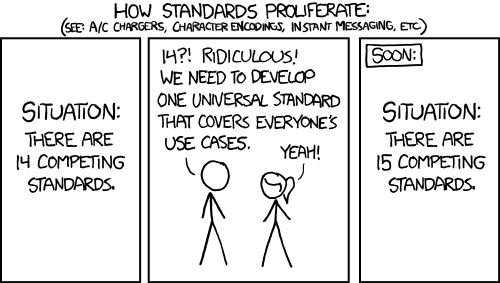
\includegraphics[width=.8\linewidth]{./gfx/xkcd-standards}
\caption
[Langlebigkeit von Standards in der IT]
{Langlebigkeit von Standards in der IT. Quelle: \url{https://xkcd.com/927/}} \label{fig:xkcd-standards}
\end{center}
\end{figure}

\begin{warnbox}[Erfolg der Allozierung prüfen]
In seltenen Fällen kann die Allozierung von Speicher fehlschlagen. Dies ist insbesondere dann der Fall, wenn nicht mehr ausreichend \emph{zusammenhängender} Speicher zur Verfügung steht, um ein Array der gewünschten Größe darin unterzubringen. In diesem Fall ist der Rückgabewert von \texttt{calloc} und \texttt{malloc} ein Null-Pointer (\ie der Wert \texttt{0}). Auf die Adresse \texttt{0} darf nicht zugegriffen werden; jeder Zugriff führt zum Programmabsturz. Daher sollte nach jedem \texttt{alloc}-Befehl eine Fehlerprüfung stattfinden. Mit dem Befehl \texttt{exit} aus der \texttt{stdlib.h} können wir etwa das Programm beenden. In Kapitel \ref{chp:OS-Link} werden wir hierzu mehr hören.

\begin{codebox}[Beispiel: Fehlerprüfung nachg Allozierung]
\begin{minted}[linenos]{c}
int * array = malloc(20);
if (!array) {
   printf("Fehler! Speicher konnte nicht alloziert werden!\n");
   exit(-1); // Programm beenden.
}
\end{minted}
\end{codebox}
\end{warnbox}

\subsection{Feldgrößen ändern: \texttt{realloc}} \label{sec:realloc}
Der Befehl \texttt{realloc} (eingebunden über den Header \texttt{stdlib.h}) ändert die Größe eines bestehenden Arrays und erhält alle Werte bei (sofern sie in noch \enquote{in das neue Array passen}). In der Regel ändert sich der Wert des Pointers auf den Beginn des Arrays nicht. Bei Vergrößerung kann es jedoch sein, dass das Array sonst mit einem anderen reservierten Speicherbereich (\eg ein anderes Array) überlappt. In diesem Fall wird \texttt{realloc} das gesamte Array an eine neue Stelle kopieren.

\begin{tcolorbox}[title=Visualisierung: Arraygrößen ändern]
Betrachten wir zuerst den Fall, in dem sich zwischen dem Ende eines zu vergrößernden Arrays und dem nächsten reservierten Speicherbereich viel Platz befindet. \texttt{realloc} wird lediglich zusätzlichen Platz reservieren und sonst keine Änderungen vornehmen.

\begin{tikzpicture}
  [ 
    cell/.style={
       text width =3mm,
       text height=3mm, 
       draw=black, 
       inner sep=1mm
    },
    ld/.style={
       draw=blue,
       shorten >=2pt,
       ->
    }
  ]
  \node (c00) at ( 0.0,1) [cell]         {\ttfamily 0};
  \node (c01) at ( 0.5,1) [cell]         {\ttfamily 0};
  \node (c02) at ( 1.0,1) [cell]         {\ttfamily 0};
  \node (c03) at ( 1.5,1) [cell]         {\ttfamily 0};
  \node (c04) at ( 2.0,1) [cell]         {\ttfamily 0};
  \node (c05) at ( 2.5,1) [cell]         {\ttfamily 0};
  \node (c06) at ( 3.0,1) [cell]         {\ttfamily 0};
  \node (c07) at ( 3.5,1) [cell]         {\ttfamily 0};
  \node (c08) at ( 4.0,1) [cell]         {\ttfamily 0};
  \node (c09) at ( 4.5,1) [cell]         {\ttfamily 0};
  \node (c10) at ( 5.0,1) [cell]         {\ttfamily 0};
  \node (c11) at ( 5.5,1) [cell]         {\ttfamily 0};
  \node (c12) at ( 6.0,1) [cell]         {\ttfamily 0};
  \node (c13) at ( 6.5,1) [cell]         {\ttfamily 0};
  \node (c14) at ( 7.0,1) [cell, blue]   {\ttfamily x};
  \node (c15) at ( 7.5,1) [cell, blue]   {\ttfamily k};
  \node (c16) at ( 8.0,1) [cell, blue]   {\ttfamily c};
  \node (c17) at ( 8.5,1) [cell, blue]   {\ttfamily d};
  \node (c18) at ( 9.0,1) [cell, blue]   {\ttfamily 0};
  \node (c19) at ( 9.5,1) [cell]         {\ttfamily 0};
  \node (c20) at (10.0,1) [cell]         {\ttfamily 0};
  \node (c21) at (10.5,1) [cell]         {\ttfamily 0};
  \node (c22) at (11.0,1) [cell]         {\ttfamily 0};
  \node (c23) at (11.5,1) [cell]         {\ttfamily 0};
  \node (c24) at (12.0,1) [cell, violet] {\ttfamily s};
  \node (c25) at (12.5,1) [cell, violet] {\ttfamily m};
  \node (c26) at (13.0,1) [cell, violet] {\ttfamily b};
  \node (c27) at (13.5,1) [cell, violet] {\ttfamily c};
  \node (c28) at (14.0,1) [cell, violet] {\ttfamily 0};
  
  \draw [decorate, decoration={brace,amplitude=7pt, mirror}, xshift=-0pt, yshift=0pt, blue]
  		( 6.75, 0.5) -- ( 9.25, 0.5) node [blue, midway, yshift=-0.5cm] 
		(braceArrayPreResize) {zu vergrößerndes Array};

  \draw [decorate, decoration={brace,amplitude=7pt, mirror}, xshift=-0pt, yshift=0pt, violet]
  		(11.75, 0.5) -- (14.25, 0.5) node [violet, midway, yshift=-0.5cm] 
		(braceArrayPreResize) {reservierter Speicher};
\end{tikzpicture}

Soll nun das Array um drei Zellen vergrößert werden, so wird es einfach \enquote{nach hinten verlängert}:

\begin{tikzpicture}
  [ 
    cell/.style={
       text width =3mm,
       text height=3mm, 
       draw=black, 
       inner sep=1mm
    },
    ld/.style={
       draw=blue,
       shorten >=2pt,
       ->
    }
  ]
  \node (c00) at ( 0.0,1) [cell]         {\ttfamily 0};
  \node (c01) at ( 0.5,1) [cell]         {\ttfamily 0};
  \node (c02) at ( 1.0,1) [cell]         {\ttfamily 0};
  \node (c03) at ( 1.5,1) [cell]         {\ttfamily 0};
  \node (c04) at ( 2.0,1) [cell]         {\ttfamily 0};
  \node (c05) at ( 2.5,1) [cell]         {\ttfamily 0};
  \node (c06) at ( 3.0,1) [cell]         {\ttfamily 0};
  \node (c07) at ( 3.5,1) [cell]         {\ttfamily 0};
  \node (c08) at ( 4.0,1) [cell]         {\ttfamily 0};
  \node (c09) at ( 4.5,1) [cell]         {\ttfamily 0};
  \node (c10) at ( 5.0,1) [cell]         {\ttfamily 0};
  \node (c11) at ( 5.5,1) [cell]         {\ttfamily 0};
  \node (c12) at ( 6.0,1) [cell]         {\ttfamily 0};
  \node (c13) at ( 6.5,1) [cell]         {\ttfamily 0};
  \node (c14) at ( 7.0,1) [cell, blue]   {\ttfamily x};
  \node (c15) at ( 7.5,1) [cell, blue]   {\ttfamily k};
  \node (c16) at ( 8.0,1) [cell, blue]   {\ttfamily c};
  \node (c17) at ( 8.5,1) [cell, blue]   {\ttfamily d};
  \node (c18) at ( 9.0,1) [cell, blue]   {\ttfamily 0};
  \node (c19) at ( 9.5,1) [cell, teal]   {\ttfamily 0};
  \node (c20) at (10.0,1) [cell, teal]   {\ttfamily 0};
  \node (c21) at (10.5,1) [cell, teal]   {\ttfamily 0};
  \node (c22) at (11.0,1) [cell]         {\ttfamily 0};
  \node (c23) at (11.5,1) [cell]         {\ttfamily 0};
  \node (c24) at (12.0,1) [cell, violet] {\ttfamily s};
  \node (c25) at (12.5,1) [cell, violet] {\ttfamily m};
  \node (c26) at (13.0,1) [cell, violet] {\ttfamily b};
  \node (c27) at (13.5,1) [cell, violet] {\ttfamily c};
  \node (c28) at (14.0,1) [cell, violet] {\ttfamily 0};
  
  \draw [decorate, decoration={brace,amplitude=7pt, mirror}, xshift=-0pt, yshift=0pt, blue]
  		( 6.75, 0.5) -- (10.75, 0.5) node [blue, midway, yshift=-0.5cm] 
		(braceArrayPreResize) {vergrößertes Array};

  \draw [decorate, decoration={brace,amplitude=7pt, mirror}, xshift=-0pt, yshift=0pt, violet]
  		(11.75, 0.5) -- (14.25, 0.5) node [violet, midway, yshift=-0.5cm] 
		(braceArrayPreResize) {reservierter Speicher};

  \draw [decorate, decoration={brace,amplitude=7pt}, xshift=-0pt, yshift=0pt, teal]
  		( 9.25, 1.4) -- (10.75, 1.4) node [teal, midway, yshift=+0.5cm] 
		(braceArrayPreResize) {Erweiterung};
\end{tikzpicture}

Bei mehr als fünf Zellen zusätzlichen Speicherbedarf entsteht jedoch ein Konflikt:

\begin{tikzpicture}
  [ 
    cell/.style={
       text width =3mm,
       text height=3mm, 
       draw=black, 
       inner sep=1mm
    },
    ld/.style={
       draw=blue,
       shorten >=2pt,
       ->
    }
  ]
  \node (c00) at ( 0.0,1) [cell]         {\ttfamily 0};
  \node (c01) at ( 0.5,1) [cell]         {\ttfamily 0};
  \node (c02) at ( 1.0,1) [cell]         {\ttfamily 0};
  \node (c03) at ( 1.5,1) [cell]         {\ttfamily 0};
  \node (c04) at ( 2.0,1) [cell]         {\ttfamily 0};
  \node (c05) at ( 2.5,1) [cell]         {\ttfamily 0};
  \node (c06) at ( 3.0,1) [cell]         {\ttfamily 0};
  \node (c07) at ( 3.5,1) [cell]         {\ttfamily 0};
  \node (c08) at ( 4.0,1) [cell]         {\ttfamily 0};
  \node (c09) at ( 4.5,1) [cell]         {\ttfamily 0};
  \node (c10) at ( 5.0,1) [cell]         {\ttfamily 0};
  \node (c11) at ( 5.5,1) [cell]         {\ttfamily 0};
  \node (c12) at ( 6.0,1) [cell]         {\ttfamily 0};
  \node (c13) at ( 6.5,1) [cell]         {\ttfamily 0};
  \node (c14) at ( 7.0,1) [cell, blue]   {\ttfamily x};
  \node (c15) at ( 7.5,1) [cell, blue]   {\ttfamily k};
  \node (c16) at ( 8.0,1) [cell, blue]   {\ttfamily c};
  \node (c17) at ( 8.5,1) [cell, blue]   {\ttfamily d};
  \node (c18) at ( 9.0,1) [cell, blue]   {\ttfamily 0};
  \node (c19) at ( 9.5,1) [cell, teal]   {\ttfamily 0};
  \node (c20) at (10.0,1) [cell, teal]   {\ttfamily 0};
  \node (c21) at (10.5,1) [cell, teal]   {\ttfamily 0};
  \node (c22) at (11.0,1) [cell, teal]   {\ttfamily 0};
  \node (c23) at (11.5,1) [cell, teal]   {\ttfamily 0};
  \node (c24) at (12.0,1) [cell, red]    {\ttfamily s};
  \node (c25) at (12.5,1) [cell, red]    {\ttfamily m};
  \node (c26) at (13.0,1) [cell, violet] {\ttfamily b};
  \node (c27) at (13.5,1) [cell, violet] {\ttfamily c};
  \node (c28) at (14.0,1) [cell, violet] {\ttfamily 0};
  
  \draw [decorate, decoration={brace,amplitude=7pt, mirror}, xshift=-0pt, yshift=0pt, blue]
  		( 6.75, 0.5) -- ( 9.25, 0.5) node [blue, midway, yshift=-0.5cm] 
		(braceArrayPreResize) {zu vergrößerndes Array};

  \draw [decorate, decoration={brace,amplitude=7pt, mirror}, xshift=-0pt, yshift=0pt, violet]
  		(11.75, 0.5) -- (14.25, 0.5) node [violet, midway, yshift=-0.5cm] 
		(braceArrayPreResize) {reservierter Speicher};

  \draw [decorate, decoration={brace,amplitude=7pt}, xshift=-0pt, yshift=0pt, teal]
  		( 9.25, 1.4) -- (12.75, 1.4) node [teal, midway, yshift=+0.5cm] 
		(braceArrayPreResize) {Gewünschte Erweiterung};

  \draw [decorate, decoration={brace,amplitude=7pt}, xshift=-0pt, yshift=0pt, red]
  		(11.75, 2.2) -- (12.75, 2.2) node [red, midway, yshift=+0.5cm] 
		(braceArrayPreResize) {Konflikt};
\end{tikzpicture}

Stattdessen wird also das Array als Ganzes an eine neue Stelle kopiert:

\begin{tikzpicture}
  [ 
    cell/.style={
       text width =3mm,
       text height=3mm, 
       draw=black, 
       inner sep=1mm
    },
    ld/.style={
       draw=blue,
       shorten >=2pt,
       ->
    }
  ]
  \node (c00) at ( 0.0,1) [cell]         {\ttfamily 0};
  \node (c01) at ( 0.5,1) [cell, teal]   {\ttfamily x};
  \node (c02) at ( 1.0,1) [cell, teal]   {\ttfamily k};
  \node (c03) at ( 1.5,1) [cell, teal]   {\ttfamily c};
  \node (c04) at ( 2.0,1) [cell, teal]   {\ttfamily d};
  \node (c05) at ( 2.5,1) [cell, teal]   {\ttfamily 0};
  \node (c06) at ( 3.0,1) [cell, blue]   {\ttfamily 0};
  \node (c07) at ( 3.5,1) [cell, blue]   {\ttfamily 0};
  \node (c08) at ( 4.0,1) [cell, blue]   {\ttfamily 0};
  \node (c09) at ( 4.5,1) [cell, blue]   {\ttfamily 0};
  \node (c10) at ( 5.0,1) [cell, blue]   {\ttfamily 0};
  \node (c11) at ( 5.5,1) [cell, blue]   {\ttfamily 0};
  \node (c12) at ( 6.0,1) [cell, blue]   {\ttfamily 0};
  \node (c13) at ( 6.5,1) [cell]         {\ttfamily 0};
  \node (c14) at ( 7.0,1) [cell]         {\ttfamily x};
  \node (c15) at ( 7.5,1) [cell]         {\ttfamily k};
  \node (c16) at ( 8.0,1) [cell]         {\ttfamily c};
  \node (c17) at ( 8.5,1) [cell]         {\ttfamily d};
  \node (c18) at ( 9.0,1) [cell]         {\ttfamily 0};
  \node (c19) at ( 9.5,1) [cell]         {\ttfamily 0};
  \node (c20) at (10.0,1) [cell]         {\ttfamily 0};
  \node (c21) at (10.5,1) [cell]         {\ttfamily 0};
  \node (c22) at (11.0,1) [cell]         {\ttfamily 0};
  \node (c23) at (11.5,1) [cell]         {\ttfamily 0};
  \node (c24) at (12.0,1) [cell, violet] {\ttfamily s};
  \node (c25) at (12.5,1) [cell, violet] {\ttfamily m};
  \node (c26) at (13.0,1) [cell, violet] {\ttfamily b};
  \node (c27) at (13.5,1) [cell, violet] {\ttfamily c};
  \node (c28) at (14.0,1) [cell, violet] {\ttfamily 0};
  
  \draw [decorate, decoration={brace,amplitude=7pt, mirror}, xshift=-0pt, yshift=0pt, blue]
  		( 0.25, 0.5) -- ( 6.25, 0.5) node [blue, midway, yshift=-0.5cm] 
		(braceArrayPreResize) {vergrößertes Array mit kopierten Daten};

  \draw [decorate, decoration={brace,amplitude=7pt, mirror}, xshift=-0pt, yshift=0pt, violet]
  		(11.75, 0.5) -- (14.25, 0.5) node [violet, midway, yshift=-0.5cm] 
		(braceArrayPreResize) {reservierter Speicher};

  \draw [decorate, decoration={brace,amplitude=7pt}, xshift=-0pt, yshift=0pt, teal]
  		( 0.25, 1.4) -- ( 2.75, 1.4) node [teal, midway, yshift=+0.5cm] 
		(braceArrayPreResize) {Kopierte Daten};
  
  \draw [decorate, decoration={brace,amplitude=7pt, mirror}, xshift=-0pt, yshift=0pt, black]
  		( 6.75, 0.5) -- ( 9.25, 0.5) node [black, midway, yshift=-0.9cm] 
		(braceArrayPreResize) {\parbox{1.7cm}{\centering alte Daten, nicht mehr reserviert}};
\end{tikzpicture}

Da die Daten des Arrays vor dem Vergrößern kopiert (im Gegensatz zu verschoben) werden, bleiben diese Werte in den Speicherzellen. Die Zellen sind aber nicht mehr reserviert. Eine folgende Anfrage, Speicher zu allozieren (\eg mit \texttt{malloc}) kann also genau diese Zellen auswählen und für neue Zwecke benutzen.
\end{tcolorbox}
\begin{tcolorbox}
Verkürzt man ein Array, so wird ebenso lediglich die Reservierung aufgehoben:

\begin{tikzpicture}
  [ 
    cell/.style={
       text width =3mm,
       text height=3mm, 
       draw=black, 
       inner sep=1mm
    },
    ld/.style={
       draw=blue,
       shorten >=2pt,
       ->
    }
  ]
  \node (c00) at ( 0.0,1) [cell]         {\ttfamily 0};
  \node (c01) at ( 0.5,1) [cell]         {\ttfamily 0};
  \node (c02) at ( 1.0,1) [cell]         {\ttfamily 0};
  \node (c03) at ( 1.5,1) [cell]         {\ttfamily 0};
  \node (c04) at ( 2.0,1) [cell]         {\ttfamily 0};
  \node (c05) at ( 2.5,1) [cell]         {\ttfamily 0};
  \node (c06) at ( 3.0,1) [cell]         {\ttfamily 0};
  \node (c07) at ( 3.5,1) [cell]         {\ttfamily 0};
  \node (c08) at ( 4.0,1) [cell]         {\ttfamily 0};
  \node (c09) at ( 4.5,1) [cell]         {\ttfamily 0};
  \node (c10) at ( 5.0,1) [cell]         {\ttfamily 0};
  \node (c11) at ( 5.5,1) [cell]         {\ttfamily 0};
  \node (c12) at ( 6.0,1) [cell]         {\ttfamily 0};
  \node (c13) at ( 6.5,1) [cell]         {\ttfamily 0};
  \node (c14) at ( 7.0,1) [cell, blue]   {\ttfamily x};
  \node (c15) at ( 7.5,1) [cell, blue]   {\ttfamily k};
  \node (c16) at ( 8.0,1) [cell, blue]   {\ttfamily c};
  \node (c17) at ( 8.5,1) [cell]         {\ttfamily d};
  \node (c18) at ( 9.0,1) [cell]         {\ttfamily 0};
  \node (c19) at ( 9.5,1) [cell]         {\ttfamily 0};
  \node (c20) at (10.0,1) [cell]         {\ttfamily 0};
  \node (c21) at (10.5,1) [cell]         {\ttfamily 0};
  \node (c22) at (11.0,1) [cell]         {\ttfamily 0};
  \node (c23) at (11.5,1) [cell]         {\ttfamily 0};
  \node (c24) at (12.0,1) [cell, violet] {\ttfamily s};
  \node (c25) at (12.5,1) [cell, violet] {\ttfamily m};
  \node (c26) at (13.0,1) [cell, violet] {\ttfamily b};
  \node (c27) at (13.5,1) [cell, violet] {\ttfamily c};
  \node (c28) at (14.0,1) [cell, violet] {\ttfamily 0};
  
  \draw [decorate, decoration={brace,amplitude=7pt, mirror}, xshift=-0pt, yshift=0pt, blue]
  		( 6.75, 0.5) -- ( 8.25, 0.5) node [blue, midway, yshift=-0.5cm] 
		(braceArrayPreResize) {verkleinertes Array};

  \draw [decorate, decoration={brace,amplitude=7pt, mirror}, xshift=-0pt, yshift=0pt, violet]
  		(11.75, 0.5) -- (14.25, 0.5) node [violet, midway, yshift=-0.5cm] 
		(braceArrayPreResize) {reservierter Speicher};

  \draw [decorate, decoration={brace,amplitude=7pt}, xshift=-0pt, yshift=0pt, black]
  		( 8.25, 1.4) -- ( 9.25, 1.4) node [black, midway, yshift=+0.5cm] 
		(braceArrayPreResize) {Freigegebener Speicher};
\end{tikzpicture}
\end{tcolorbox}

In der Syntax orientiert sich \texttt{realloc} am Befehl \texttt{malloc}:

\begin{codebox}[Syntax: \texttt{realloc}]
\begin{minted}{c}
pointer = realloc(pointer, AnzahlBytesNeu);
\end{minted}
\end{codebox}

Dabei ist \texttt{pointer} die Adresse des Arrays, dessen Größe geändert werden soll und \texttt{AnzahlBytesNeu} die gewünschte Größe des neuen Arrays.

Wie wir gesehen haben kann sich die Adresse des Arrays (also sein Startpunkt im Speicher) bei Größenänderung verschieben. Daher müssen wir auch hier das Ergebnis speichern; wir aktualisieren also den Wert der Variablen \texttt{pointer}. Natürlich kann es auch geschehen, dass die Größenänderung fehlschlägt (etwa, wenn ein zu großer Speicherbereich angefragt wird). In diesem Fall ist der Rückgabewert von \texttt{realloc} gleich \texttt{0}. Es gehört zum guten Stil, auf solche Fehler mit \mintinline{c}{if} zu reagieren.

Betrachten wir folgendes Beispiel aus der \href{https://en.cppreference.com/w/c/memory/realloc}{CPP-Referenz}:

\begin{codebox}[Beispiel: \texttt{realloc}]
\begin{minted}[linenos]{c}
#include <stdio.h>
#include <stdlib.h>
 
int main(void) {
    int *pa = malloc(10 * sizeof(*pa)); // allocate an array of 10 int
    if (pa) {
        printf("%ld bytes allocated. Storing ints: ", 10 * sizeof(int));
        for(int n = 0; n < 10; ++n) {printf("%d ", pa[n] = n);}
    }
    
    // reallocate array to a larger size
    int *pb = realloc(pa, 1000000 * sizeof(*pb)); 
    if (pb) {
        printf("\n%ld bytes allocated, first 10 ints are: ", 
               1000000 * sizeof(int)
        );
        for(int n = 0; n < 10; ++n) {printf("%d ", pb[n]);} // show the array
        free(pb);
    } else { // if realloc failed, the original pointer needs to be freed
        free(pa);
    }
}
\end{minted}
{\normalfont(Mit leichten Abwandlungen übernommen von \url{https://en.cppreference.com/w/c/memory/realloc})}
\end{codebox}

\begin{cmdbox}[Ausführungsbeispiel: \texttt{realloc}]
40 bytes allocated. Storing ints: 0 1 2 3 4 5 6 7 8 9 \\
4000000 bytes allocated, first 10 ints are: 0 1 2 3 4 5 6 7 8 9 0
\end{cmdbox}

In Zeile 5 wird versucht, mit \texttt{malloc} Speicher für ein Array zu reservieren, das 10 \mintinline{c}{int}-Werte fassen kann. Beachten Sie hier auch die Verwendung des \mintinline{c}{sizeof}-Operators: Abgefragt wird hier die Speichergröße von \texttt{*pa}. Die Variable \texttt{pa} ist ein Pointer auf \mintinline{c}{int}; damit ist die dereferenzierte Variable \texttt{*pa} selbst ein Ausdruck vom Typ \mintinline{c}{int}.

\emph{Nur wenn diese Allozierung erfolgreich war}, wird das Array mit Werten befüllt und diese Werte zugleich auch auf dem Bildschirm ausgebeben. Beachten Sie hierbei die \texttt{printf}-Anweisung in Zeile 8: Ausgegeben wird der Ausdruck \texttt{pa[n] = n}. Dieser Ausdruck ist zunächst eine \emph{Wertzuweisung} -- in \texttt{pa[n]} wird also der Wert \texttt{n} gespeichert. Zugleich ist das \enquote{Ergebnis} dieser Wertzuweisung der zugewiesene Wert selbst -- \texttt{printf} gibt also den Wert von \texttt{n} aus.

In Zeile 12 versuchen wir nun, das Array so zu vergrößern, dass es \mbox{1\;000\;000} \mintinline{c}{int}-Werte halten kann. Wenn dies gelingt, wird die Variable \texttt{pb} einen von null verschiedenen Wert haben; der Pointer \texttt{pa} dagegen ist \emph{möglicherweise nicht mehr gültig}!

Bei Erfolg dieser Vergrößerung können wir nun über \texttt{pb} auf die Werte des Arrays zugreifen, und finden die Elemente, die wir zuvor über \texttt{pa} gespeichert hatten. Obwohl im Programm zwei verschiedene Pointer-Variablen benutzt werden, existiert nur ein einzeiges Array.

Wie üblich müssen \emph{dynamische Arrays} mit \texttt{free} freigegeben werden. War die Vergrößerung mit \texttt{realloc} erfolgreich, so muss dies über den Pointer \texttt{pb} geschehen, da \texttt{pa} möglicherweise \enquote{ins Leere} zeigt. Konnte dagegen das Array nicht so weit vergrößert werden, so existiert weiterhin das Array mit der Adresse \texttt{pa}. Daher schreiben wir für diesen Fall in Zeile 20 \texttt{free(pa)}.

\subsection{Heap und Stack} \label{sec:HeapStack}
In Abschnitt \ref{sec:Arrays} haben wir \emph{automatische Arrays} kennen gelernt. Später in Abschnitt \ref{sec:dynArrays} haben wir \emph{dynamische Arrays} eingeführt. Während der Zugriff auf die Array-Elemente für beide Arten gleich ist, bestehen doch Unterschiede. \emph{Automatische} Arrays sind in ihrer Größe fest und können nach dem Anlegen nicht mehr verändert werden. Dafür müssen wir uns nicht um die Freigabe des Speichers nach Benutzung kümmern. Für \emph{dynamische} Arrays gilt in dieser Hinsicht das Gegenteil.

Um grob zu verstehen, warum das so ist, müssen Sie wissen, dass der Arbeitsspeicher in mehrere Segmente geteilt wird. 

Ein erstes Segment ist der Code-Bereich. Hier liegt der Maschinencode, also die Folge von Bytes, die den Prozessor Anweisen, unsere Anweisungen auszuführen. 

Hieran schließt sich der \emph{Heap} (englisch: Haufen) an. Es ist ein Bereich, auf den mehr oder minder \enquote{wahllos} zugegriffen werden kann: beliebige Schnitte des Heaps können reserviert und wieder freigegeben werden, ohne eine bestimmte Struktur oder Reihenfolge einhalten zu müssen. Auf dem Heap \enquote{leben} die dynamischen Arrays. Da im allgemeinen nicht vorhergesehen werden kann, wie sich ein dynamisches Array verhält, macht es keinen Sinn, diese geordnet im Speicher unterbringen zu wollen. Zu jeder Zeit könnte ein \texttt{realloc} eine geordnete Struktur aufbrechen. Die reservierten Speicherbereiche liegen also wirklich wie ein ungeordneter Haufen vor.

Der \emph{Stack} dagegen ist eine geordnete Speicherstruktur: Hier liegen alle Werte dicht an dicht, wie Schichten eines geordneten Stapels. Dies ist nur möglich, wenn die einzelnen Schichten nicht ihre Größe ändern (und damit Lücken hinterlassen oder andere Schichten zum nachrücken zwingen). Neue Elemente können nur \enquote{oben auf den Stack gelegt} werden. Zum Freigeben des Speichers muss in umgekehrter Reihenfolge vorgegangen werden, der Stack wird \enquote{von oben nach unten} freigegeben. Auf dem Stack \enquote{leben} die automatischen Variablen, \ie Arrays wie in Abschnitt \ref{sec:Arrays} gezeigt, aber auch die \enquote{normalen Variablen}, die nur einen einzelnen Wert halten können.

\begin{tcolorbox}[title=Visualisierung: Heap und Stack]
\begin{tikzpicture}
\footnotesize
\node (code) 
	[text height=3mm, text depth=3mm, text width=.2\linewidth, fill=red!50!white]
	{Code};
\node (heap) 
	[text height=3mm, text depth=3mm, text width=.3\linewidth, fill=green!50!white, right=0pt of code] 
	{Heap};
\node (stack) 
	[text height=3mm, text depth=3mm, text width=.2\linewidth, fill=blue!50!white,  right=0pt of heap] 
	{Stack};
	
\node (tcode) 
	[below=2mm of code, text width=.18\linewidth, font=\rightskip0pt plus 1fil]
	{Programmcode -- kompilierte Datei};
\node (theap) 
	[below=2mm of heap, text width=.23\linewidth, font=\rightskip0pt plus 1fil]
	{Dynamische Speicherverwaltung};
\node (tstack) 
	[below=2mm of stack,text width=.18\linewidth, font=\rightskip0pt plus 1fil]
	{Automatische Variablen};
\end{tikzpicture}
%\\
\hspace{10pt}
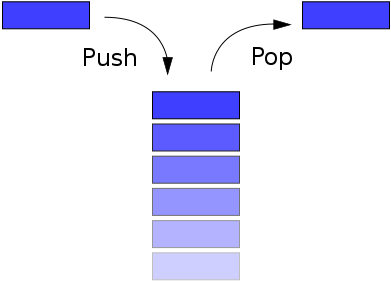
\includegraphics[width=.2\linewidth]{./gfx/Stack}
\end{tcolorbox}

Da der Stack eine so regelmäßige Gestalt hat, kann die Verwaltung automatisiert vom Betriebssystem übernommen werden. Wir müssen lediglich die Variablen deklarieren, jedoch nicht explizit Speicherplatz allozieren oder freigeben.

\begin{warnbox}[Keine dynamischen Operationen an automatischen Variablen]
Operationen der dynamischen Speicherverwaltung (insbesondere die Befehle \texttt{realloc} und \texttt{free}) sind auf dem Stack nicht erlaubt. Daher darf \emph{niemals} die Größe eines automatischen Arrays mit \texttt{realloc} geändert werden und auch \emph{niemals} sein Speicher mit \texttt{free} freigegeben werden. Der Versuch, dies zu tun führt sofort zum Programmabsturz.
\end{warnbox}


\subsection{C++} \label{sec:ArrayCPP}
\begin{plusbox}
Wie üblich stehen auch in C++ alle soeben gezeigten Mittel zur Verfügung. Automatische Arrays werden ebenso angelegt wie in C. Für \emph{dynamische Arrays} dagegen sollten nicht mehr \texttt{malloc}, \texttt{calloc} und \texttt{free} verwendet werden, sondern die Operatoren \mintinline{c++}{new} und \mintinline{c++}{delete}.

Die Syntax lautet:

\begin{codebox}[Syntax: \texttt{new} und \texttt{delete}]
\begin{minted}{c++}
pointer = new datatype [AnzahlFelder];
...
delete pointer;
\end{minted}
\end{codebox}

Auf die Unterschiede kann an dieser Stelle leider nicht im Detail eingegangen werden.

Stattdessen sei hier vermerkt, dass die C++ Standard Library eine Vielzahl von Mitteln zur Verfügung stellt, die den \emph{direkten Umgang} mit Pointern unnötig machen. Diese Mittel werden in einem eigenen Kurs vorgestellt und sind den C-Arrays \idR klar vorzuziehen.
\end{plusbox}

\subsection{mehrdimensionale dynamische Arrays}
In Abschnitt \ref{sec:MultiDimArray} haben wir bereits gesehen, wie mehrdimensionale Objekte wie Tabellen im Speicher organisiert werden können. An dieser Stelle möchte ich zwei Techniken besprechen, die solche Objekte auch mit dynamischen Arrays verfügbar machen.

\subsubsection{Geplättete Listen}
Der sicher einfachste Weg ist es, eine Tabelle (oder sein höherdimensionales Objekt) zu \enquote{plätten}, also die einzelnen Listen, aus denen es besteht, hintereinander im Speicher anzuordnen. In diesem Fall muss zwar für jeden Zugriff aus den \enquote{Koordinaten} (also \eg Spalten- und Zeilennummern der Tabelle) ein Index berechnet werden. Der sonstige \emph{Overhead} (Verwaltungsaufwand) hält sich jedoch in Grenzen.

Folgendes Beispiel erzeugt eine Tabelle, deren Maße vom User bestimmt werden, und befüllt die Zellen mit ihren Indizes. Anschließend wird die Tabelle auf dem Bildschirm ausgegeben:

\begin{codebox}[Beispiel: Tabelle mit dynamischem Array]
\begin{minted}[linenos]{c}
#include <stdio.h>
#include <stdlib.h>
 
int main(void) {
  int width = -1, height = -1, i, r, c;
  
  // Usereingaben
  printf("Bitte geben Sie die Breite der Tabelle ein:\n");
  scanf("%d", &width);
  
  printf("Bitte geben Sie die Höhe der Tabelle ein:\n");
  scanf("%d", &height);
  
  if ((height <= 0) || (width <= 0)) {
    printf("Ungültige Eingabe -- Programm wird beendet.\n");
    exit(-1);
  }
  
  // Speicher für Tabelle allozieren
  int * table = malloc(width * height * sizeof(*table));
  if (!table) {
    printf("Allozierung fehlgeschlagen -- Programm wird beendet.\n");
    exit(-1);
  }
  
  // Tabelleninhalt schreiben
  for (i = 0; i < width * height; i++) {
    table[i] = i;
  }
  
  // Tabelle auf dem Bildschirm ausgeben
  for   (r = 0; r < height; r++) {
    for (c = 0; c < width;  c++) {
      printf("%3d\t", table[r * width + c]);
    }
    printf("\n");
  }
  
  // Speicher freigeben
  free(table);
}
\end{minted}
\end{codebox}

\begin{cmdbox}[Ausgabebeispiel: Tabelle mit dynamischem Array]
\begin{minted}{text}
Bitte geben Sie die Breite der Tabelle ein:
5
Bitte geben Sie die Höhe der Tabelle ein:
3
  0       1       2       3       4
  5       6       7       8       9
 10      11      12      13      14
\end{minted}
\end{cmdbox}

Das Array \texttt{table}, in dem wir unsere Tabelle geplättet ablegen, kann mit \texttt{realloc} vergrößert und verkleinert werden. Soll die Struktur der Tabelle erhalten bleiben, können wir auf dieses Mittel allerdings nicht zurückgreifen.

Ausgehend vom obigen Code (\emph{Tabelle mit dynamischem Array}) ändern wir das Ende des Codes ab und versuchen, ab Zeile 39 die Tabelle um eine Spalte zu verbreitern:

\begin{warnbox}[Beispiel: Tabelle vergrößern mit dynamischem Array -- (fehlerhafter Code),leftupper=7mm]
\begin{minted}[linenos, firstnumber=39]{c}
  // Tabelle verbreitern
  width++;
  int * newTable = realloc(table, width * height * sizeof(*table));
  if (!newTable) {
    printf("Allozierung fehlgeschlagen -- Programm wird beendet.\n");
    free(table);
    exit(-1);
  } else {
    table = newTable;
  }
  
  // Tabelle auf dem Bildschirm ausgeben
  printf("\nVerbreiterte Tabelle:\n");
  for   (r = 0; r < height; r++) {
    for (c = 0; c < width;  c++) {
      printf("%3d\t", table[r * width + c]);
    }
    printf("\n");
  }
  
  // Speicher freigeben
  free(table);
}
\end{minted}
\end{warnbox}

Die Ausgabe lautet:

\begin{cmdbox}[Ausgabebeispiel: Tabelle vergrößern mit dynamischem Array -- (fehlerhafter Code)]
\begin{minted}{text}
Bitte geben Sie die Breite der Tabelle ein:
5
Bitte geben Sie die Höhe der Tabelle ein:
3
  0       1       2       3       4
  5       6       7       8       9
 10      11      12      13      14

Verbreiterte Tabelle:
  0       1       2       3       4       5
  6       7       8       9      10      11
 12      13      14       0       0       0

\end{minted}
\end{cmdbox}

Um dieses Verhalten zu verstehen, müssen wir uns das Speicherbild ansehen:

\begin{tcolorbox}[title=Visualisierung: Abbild der Tabelle im Speicher]
Bis Zeile 39 des Codes liegen die Tabellen-Zeilen dicht aneinander:

\begin{tikzpicture}
  [ 
    cell/.style={
       text width =3mm,
       text height=3mm, 
       draw=black, 
       inner sep=1mm
    },
    ld/.style={
       draw=blue,
       shorten >=2pt,
       ->
    }
  ]
  \node (c00) at ( 0.0,1) [cell]         {\ttfamily  0};
  \node (c01) at ( 0.5,1) [cell, blue]   {\ttfamily  0};
  \node (c02) at ( 1.0,1) [cell, blue]   {\ttfamily  1};
  \node (c03) at ( 1.5,1) [cell, blue]   {\ttfamily  2};
  \node (c04) at ( 2.0,1) [cell, blue]   {\ttfamily  3};
  \node (c05) at ( 2.5,1) [cell, blue]   {\ttfamily  4};
  \node (c06) at ( 3.0,1) [cell, blue]   {\ttfamily  5};
  \node (c07) at ( 3.5,1) [cell, blue]   {\ttfamily  6};
  \node (c08) at ( 4.0,1) [cell, blue]   {\ttfamily  7};
  \node (c09) at ( 4.5,1) [cell, blue]   {\ttfamily  8};
  \node (c10) at ( 5.0,1) [cell, blue]   {\ttfamily  9};
  \node (c11) at ( 5.5,1) [cell, blue]   {\ttfamily 10};
  \node (c12) at ( 6.0,1) [cell, blue]   {\ttfamily 11};
  \node (c13) at ( 6.5,1) [cell, blue]   {\ttfamily 12};
  \node (c14) at ( 7.0,1) [cell, blue]   {\ttfamily 13};
  \node (c15) at ( 7.5,1) [cell, blue]   {\ttfamily 14};
  \node (c16) at ( 8.0,1) [cell]         {\ttfamily  0};
  \node (c17) at ( 8.5,1) [cell]         {\ttfamily  0};
  \node (c18) at ( 9.0,1) [cell]         {\ttfamily  0};
  \node (c19) at ( 9.5,1) [cell]         {\ttfamily  0};
  \node (c20) at (10.0,1) [cell]         {\ttfamily  0};
  \node (c21) at (10.5,1) [cell]         {\ttfamily  0};
  \node (c22) at (11.0,1) [cell]         {\ttfamily  0};
  \node (c23) at (11.5,1) [cell]         {\ttfamily  0};
  \node (c24) at (12.0,1) [cell]         {\ttfamily  0};
  \node (c25) at (12.5,1) [cell]         {\ttfamily  0};
  \node (c26) at (13.0,1) [cell]         {\ttfamily  0};
  \node (c27) at (13.5,1) [cell]         {\ttfamily  0};
  \node (c28) at (14.0,1) [cell]         {\ttfamily  0};
  
  \draw [decorate, decoration={brace,amplitude=7pt, mirror}, xshift=-0pt, yshift=0pt, blue]
  		( 0.25, -0.3) -- ( 7.75, -0.3) node [blue, midway, yshift=-0.5cm] 
		(braceArrayPreResize) {Array \texttt{table}};

  \draw [decorate, decoration={brace,amplitude=7pt, mirror}, xshift=-0pt, yshift=0pt, blue]
  		( 0.25, 0.5) -- ( 2.75, 0.5) node [blue, midway, yshift=-0.5cm] 
		(braceArrayPreResize) {Zeile 1};
  \draw [decorate, decoration={brace,amplitude=7pt, mirror}, xshift=-0pt, yshift=0pt, blue]
  		( 2.75, 0.5) -- ( 5.25, 0.5) node [blue, midway, yshift=-0.5cm] 
		(braceArrayPreResize) {Zeile 2};
  \draw [decorate, decoration={brace,amplitude=7pt, mirror}, xshift=-0pt, yshift=0pt, blue]
  		( 5.25, 0.5) -- ( 7.75, 0.5) node [blue, midway, yshift=-0.5cm] 
		(braceArrayPreResize) {Zeile 3};
\end{tikzpicture}

Mit \texttt{realloc} erweitern wir unseren Speicher um weitere 3 Elemente, um so Platz für eine zusätzliche Spalte zu haben. Wie in Abschnitt \ref{sec:realloc} gezeigt, wird dieser Platz \emph{am Ende des Arrays} angehängt. Wegen \texttt{width++} in Code-Zeile 48 lesen wir ab jetzt aber Ketten von \emph{6 Speicherstellen} als eine Zeile, und erhalten eine zersetzte Tabelle:

\begin{tikzpicture}
  [ 
    cell/.style={
       text width =3mm,
       text height=3mm, 
       draw=black, 
       inner sep=1mm
    },
    ld/.style={
       draw=blue,
       shorten >=2pt,
       ->
    }
  ]
  \node (c00) at ( 0.0,1) [cell]         {\ttfamily  0};
  \node (c01) at ( 0.5,1) [cell, blue]   {\ttfamily  0};
  \node (c02) at ( 1.0,1) [cell, blue]   {\ttfamily  1};
  \node (c03) at ( 1.5,1) [cell, blue]   {\ttfamily  2};
  \node (c04) at ( 2.0,1) [cell, blue]   {\ttfamily  3};
  \node (c05) at ( 2.5,1) [cell, blue]   {\ttfamily  4};
  \node (c06) at ( 3.0,1) [cell, blue]   {\ttfamily  5};
  \node (c07) at ( 3.5,1) [cell, blue]   {\ttfamily  6};
  \node (c08) at ( 4.0,1) [cell, blue]   {\ttfamily  7};
  \node (c09) at ( 4.5,1) [cell, blue]   {\ttfamily  8};
  \node (c10) at ( 5.0,1) [cell, blue]   {\ttfamily  9};
  \node (c11) at ( 5.5,1) [cell, blue]   {\ttfamily 10};
  \node (c12) at ( 6.0,1) [cell, blue]   {\ttfamily 11};
  \node (c13) at ( 6.5,1) [cell, blue]   {\ttfamily 12};
  \node (c14) at ( 7.0,1) [cell, blue]   {\ttfamily 13};
  \node (c15) at ( 7.5,1) [cell, blue]   {\ttfamily 14};
  \node (c16) at ( 8.0,1) [cell, teal]   {\ttfamily  0};
  \node (c17) at ( 8.5,1) [cell, teal]   {\ttfamily  0};
  \node (c18) at ( 9.0,1) [cell, teal]   {\ttfamily  0};
  \node (c19) at ( 9.5,1) [cell]         {\ttfamily  0};
  \node (c20) at (10.0,1) [cell]         {\ttfamily  0};
  \node (c21) at (10.5,1) [cell]         {\ttfamily  0};
  \node (c22) at (11.0,1) [cell]         {\ttfamily  0};
  \node (c23) at (11.5,1) [cell]         {\ttfamily  0};
  \node (c24) at (12.0,1) [cell]         {\ttfamily  0};
  \node (c25) at (12.5,1) [cell]         {\ttfamily  0};
  \node (c26) at (13.0,1) [cell]         {\ttfamily  0};
  \node (c27) at (13.5,1) [cell]         {\ttfamily  0};
  \node (c28) at (14.0,1) [cell]         {\ttfamily  0};
  
  \draw [decorate, decoration={brace,amplitude=7pt, mirror}, xshift=-0pt, yshift=0pt, blue]
  		( 0.25, -0.3) -- ( 9.25, -0.3) node [blue, midway, yshift=-0.5cm] 
		(braceArrayPreResize) {Array \texttt{table}};

  \draw [decorate, decoration={brace,amplitude=7pt, mirror}, xshift=-0pt, yshift=0pt, blue]
  		( 0.25, 0.5) -- ( 3.25, 0.5) node [blue, midway, yshift=-0.5cm] 
		(braceArrayPreResize) {Zeile 1};
  \draw [decorate, decoration={brace,amplitude=7pt, mirror}, xshift=-0pt, yshift=0pt, blue]
  		( 3.25, 0.5) -- ( 6.25, 0.5) node [blue, midway, yshift=-0.5cm] 
		(braceArrayPreResize) {Zeile 2};
  \draw [decorate, decoration={brace,amplitude=7pt, mirror}, xshift=-0pt, yshift=0pt, blue]
  		( 6.25, 0.5) -- ( 9.25, 0.5) node [blue, midway, yshift=-0.5cm] 
		(braceArrayPreResize) {Zeile 3};

  \draw [decorate, decoration={brace,amplitude=7pt}, xshift=-0pt, yshift=0pt, teal]
  		( 7.75, 1.4) -- ( 9.25, 1.4) node [teal, midway, yshift=+0.5cm] 
		(braceArrayPreResize) {neu reservierter Speicher};
\end{tikzpicture}
\end{tcolorbox}

(Wenn dagegen nur eine Zeile an die Tabelle angehängt werden soll, funktioniert dieses Beispiel mit \texttt{realloc} genau wie erwartet, da neue Zeilen immer \emph{am Ende} der \enquote{geplätteten Liste} angehängt werden.

Um nun auch Spalten anhängen zu können, müssen wir manuell ein neues Array erstellen und alle Tabellen-Einträge an die richtigen Stellen kopieren. Wir gehen wieder vom Beispiel \emph{Tabelle mit dynamischem Array} aus und ergänzen ab Zeile 39:

\begin{codebox}[Beispiel: Tabelle vergrößern mit dynamischem Array -- (korrekter Code)]
\begin{minted}[linenos, firstnumber=39]{c}
  // neue Tabelle anlegen
  int * newTable = calloc((width + 1) * height, sizeof(*table));
  if (!newTable) {
    printf("Allozierung fehlgeschlagen -- Programm wird beendet.\n");
    exit(-1);
  }
  
  // Tabelleninhalt kopieren
  for   (r = 0; r < height; r++) {
    for (c = 0; c < width;  c++) {
      newTable[r * (width + 1) + c] = table[r * width + c];
    }
  }
  
  // Speicher der alten Tabelle freigeben, Variablen aktualisieren
  free(table);
  table = newTable;
  width++;
  
  // Tabelle auf dem Bildschirm ausgeben
  printf("\nVerbreiterte Tabelle:\n");
  for   (r = 0; r < height; r++) {
    for (c = 0; c < width;  c++) {
      printf("%3d\t", table[r * width + c]);
    }
    printf("\n");
  }
  
  // Speicher freigeben
  free(table);
}
\end{minted}
\end{codebox}

\begin{cmdbox}[Ausgabebeispiel: Tabelle vergrößern mit dynamischem Array -- (korrekter Code)]
\begin{minted}{text}
Bitte geben Sie die Breite der Tabelle ein:
5
Bitte geben Sie die Höhe der Tabelle ein:
3
  0       1       2       3       4
  5       6       7       8       9
 10      11      12      13      14

Verbreiterte Tabelle:
  0       1       2       3       4       0
  5       6       7       8       9       0
 10      11      12      13      14       0
\end{minted}
\end{cmdbox}

\subsubsection{Pointer zweiter und tieferer Ebene}
Wir haben bereits festgestellt, dass sich eine Tabelle auch als \emph{Liste von Listen} auffassen lässt. Listen werden mit Pointern verwaltet. Die Sprache C erlaubt auch, \emph{Pointer auf Pointer} anzulegen. Diesem Gedanken folgend wollen wir eine alternative Darstellungsmöglichkeit von Tabellen diskutieren:

\begin{codebox}[Beispiel: Tabelle Pointer zweiter Ebene]
\begin{minted}[linenos]{c}
#include <stdio.h>
#include <stdlib.h>
 
int main(void) {
  int width  = -1, height = -1, r, c;
  
  // Usereingaben
  printf("Bitte geben Sie die Breite der Tabelle ein:\n"); scanf("%d", &width);
  printf("Bitte geben Sie die Höhe der Tabelle ein:\n");   scanf("%d", &height);
  
  if ((height <= 0) || (width <= 0)) {
    printf("Ungültige Eingabe -- Programm wird beendet.\n");
    exit(-1);
  }
  
  // Speicher für Tabelle allozieren
  int ** table = malloc(height * sizeof(*table));         // Liste der Zeilen
  if (!table) {
    printf("Allozierung fehlgeschlagen -- Programm wird beendet.\n");
    exit(-1);
  }
  for (r = 0; r < height; r++) {
    table[r] = malloc(  width * sizeof(*(table[r]))  );   // Zeilen selbst
  }
  
  // Tabelleninhalt schreiben
  for   (r = 0; r < height; r++) {
    for (c = 0; c < width;  c++) {
      table[r][c] = r * width + c;
    }
  }
  
  // Tabelle auf dem Bildschirm ausgeben
  for   (r = 0; r < height; r++) {
    for (c = 0; c < width;  c++) {
      printf("%3d\t", table[r][c]);
    }
    printf("\n");
  }
  
  // Speicher freigeben
  for (r = 0; r < height; r++) {free(table[r]);}
  free(table);
}
\end{minted}
\end{codebox}

Die Ausgabe ist dieselbe wie im vorigen Beispiel (\emph{Tabelle mit dynamischem Array}); \enquote{unter der Haube} sieht es jedoch bedeutend anders aus.

Zeile 17 deklariert einen \mintinline{c}{int **}, also einen \emph{Pointer auf einen \mintinline{c}{int *}}. Diese Variable \texttt{table} verweist also nicht auf den Speicherbereich, in dem die Tabellendaten selbst liegen, sondern auf Punkte im Speicher, die angeben, wo die einzelnen Zeilen der Tabelle zu finden sind.

Für jeden Eintrag in dieser Liste aus Pointern wird nun nochmal ein eigener Speicherbereich alloziert, der die tatsächlichen Tabellenwerte aufnehmen kann (Zeilen 22-24).

Mit diesem aufwändigeren Aufbau der Speicherstruktur können wir nun etwas komfortabler auf die Tabellenelemente zugreifen. In Zeile 29 wird \texttt{table[r][c]} beschrieben, wir geben also direkt den Zeilenindex \texttt{r} und den Spaltenindex \texttt{c} an, ohne einen geplätteten Index berechnen zu müssen. Halten Sie sich vor Augen: \texttt{table} ist ein \mintinline{c}{int **}. Damit liefert der Zugriff \texttt{table[r]} den Wert mit dem Index \texttt{r} aus der \emph{Liste der Listen}, also einen Pointer auf die Zeile \texttt{r}. Auf diese Liste kann nun mit dem Spaltenindex \texttt{c} zugegriffen werden.

Insgesamt haben wir also \texttt{r + 1} Listen, die die Tabelle aufbauen (\texttt{r} Listen für die Inhalte der Zeilen selbst und eine Liste, die angibt, wo im Speicher diese Zeilen zu finden sind). Alle diese Listen müssen natürlich auch wieder freigegeben werden. Hierzu dienen die Zeilen 42 und 43. Wichtig ist, dies in \emph{umgekehrter Reihenfolge des Anlegens} zu tun. Nach einem \texttt{free} \enquote{existiert} ein Array nicht mehr und ein Zugriff darauf darf eigentlich nicht mehr stattfinden. Wenn wir also die Zeilen 42 und 43 vertauschen, würden in der \mintinline{c}{for}-Schleife verbotene Zugriffe auf \texttt{table} stattfinden und möglicherweise den Programmabsturz hervorrufen.

Wollen wir diese Tabelle vergrößern, so gilt es, zwei Fälle zu unterscheiden: Eine Änderung der Zeilen-Zahl oder der Spalten-Zahl. Wenn wir Zeilen hinzufügen, reicht es, lediglich \texttt{table} mit \texttt{realloc} zu vergrößern und mit \texttt{malloc} Platz für diese neuen Zeilen zu allozieren. Für zusätzliche Spalten müssen wir jede Liste \texttt{table[r]} mit \texttt{realloc} vergrößern. Zum Verkleinern solcher Strukturen müssen Sie auch darauf achten, dass wegfallende Zeilen mit \texttt{free(table[r])} freigegeben werden müssen.

\begin{hintbox}[Geplättete Listen bevorzugen]
Wie Sie sehen ist die Verwaltung von Listen mit Pointern zweiter oder höherer Ebene komplexer und bietet mehr Fehlerquellen. Im Allgemeinen sind daher \enquote{geplättete Listen} zu bevorzugen. Relevant kann diese Technik aber dort werden, wo sie keine vollständige, \enquote{rechteckige} Tabelle beschreiben, sondern wo jede Zeile eine andere Länge hat. Für diesen Fall müssen Sie natürlich noch ein zusätzliches Array anlegen, in dem Sie die Längen der Zeilen speichern.
\end{hintbox}

\begin{hintbox}[Reihenfolge der Dimensionen frei wählbar]
In den obigen Beispielen folgte ich der Konvention \enquote{Zeilen zuerst, Spalten später}. Es gibt aber keine zwingenden Gründe hierfür; Sie können die obigen Beispiele leicht so anpassen, dass die Reihenfolge von Zeilen und Spalten vertauscht werden. Die Berechnung der geplätteten Indizes kann gleich bleiben, oder nach der Formel
\[ \mathtt{Index = c * height + r} \]
stattfinden. Dies entspricht einer Spaltenweisen Anordnung im Speicher.

Für welche Anordnung Sie sich auch entscheiden: Behalten Sie eine einmal gewählte Konvention bei, da Sie sonst durch die Verwechslung von Spalten und Zeilen viele Fehler machen werden.

Die hier gezeigten Konventionen orientieren sich an den Gewohnheiten der Mehrheit der ProgrammiererInnen. Für die Arbeit in Teams ist diese Reihenfolge also zu bevorzugen.
\end{hintbox}

\section{C-Strings} \label{sec:string}
Bisher haben wir fast ausschließlich mit Zahlenwerten gearbeitet. Wie wir in Abbildung \ref{fig:ASCII} gesehen haben, sind Buchstaben aber nur \enquote{Interpretationsweisen} von Ganzzahlen. Texte -- Zeichenketten, oder englisch: \emph{Strings} -- lassen sich also mit Ganzzahl-Arrays behandeln. Um diese (häufig auftretende) Aufgabe zu erleichtern bringt die Sprache C einige Mittel für den Umgang mit Strings mit.

\subsection{spezielle Syntax-Elemente}
Für einfache Aufgaben steht uns ein Vorrat aus 256 verschiedenen Zeichen zur Verfügung. Dies ist genau der Wertebereich des Datentyps \mintinline{c}{char} (von englisch: \emph{character}, Buchstabe oder Zeichen). Wir verwenden also \mintinline{c}{char}-Arrays zur Arbeit mit Strings.

Es ist zwar möglich, jeden Buchstaben in der ASCII-Tabelle nachzuschlagen und manuell den zugehörigen Zahlenwert zuzuweisen; jedoch wäre dies reichlich aufwändig und fehleranfällig. Stattdessen können wir auch \texttt{'}einfache Anführungszeichen\texttt{'} benutzen, um \enquote{der Zeichencode für das eingeschlossene Zeichen} auszudrücken.

\begin{codebox}[Beispiel: ASCII-Codes]
\begin{minted}[linenos]{c}
#include <stdio.h>

int main () {
  printf("Der ASCII-Code von 'a' ist %d.\n", 'a');
}
\end{minted}
\end{codebox}

Der Format-String erwartet eine Dezimalzahl (\texttt{\%d}). Um diesen Platzhalter auszufüllen wird der Ausdruck \texttt{'a'} angeboten. Statt also eine (nicht existente) Variable \texttt{a} auszugeben wird der ASCII-Code des Zeichens \texttt{a} gelesen. Entsprechend lautet die Ausgabe:

\begin{cmdbox}[Ausführungsbeispiel: ASCII-Codes]
Der ASCII-Code von 'a' ist 97.
\end{cmdbox}

\begin{hintbox}[Regelmäßigkeit von ASCII-Codes]
Die Anordnung der Zeichen im ASCII-Vorrat ist nicht zufällig. Ein nützliches Ergebnis dieser Anordnung ist, dass sich die Bitmuster von Groß- und Kleinbuchstaben in genau einem Bit unterscheiden. Es ist also möglich, \enquote{auf den ersten Blick} festzustellen, ob eine bestimmte Folge von 1en und 0en einen großen oder einen kleinen Buchstaben beschreibt.

Da Buchstaben nur Interpretationsweisen von Zahlen sind, kann mit diesen auch gerechnet werden wie mit normalen Ganzzahlen. Insbesondere beschreibt der Ausdruck
\begin{center}
\texttt{'a' - 'A'}
\end{center}
damit auch den Abstand zwischen Groß- und Kleinbuchstaben. Der Wert dieses Ausdrucks kann zu jedem Großbuchstaben addiert werden um den entsprechenden Kleinbuchstaben zu finden; umgekehrt wandelt die Subtraktion einen Kleinbuchstaben in einen Großbuchstaben um.
\end{hintbox}

Mit diesem Mittel können wir bereits ein \mintinline{c}{char}-Array anlegen und einen Text darin ablegen:

\begin{codebox}[Beispiel: Wertzuweisung Strings (1)]
\begin{minted}[linenos]{c}
#include <stdio.h>

int main () {
  char string[] = {
    'D', 'u', 'n', 'e', ' ', 'b', 'y', ' ', 
    'F', 'a', 'n', 'k', ' ', 'H', 'e', 'r', 'b', 'e', 'r', 't', 0};
}
\end{minted}
\end{codebox}

Damit legen wir ein automatisches Array namens \texttt{string} an, und speichern darin den Text \texttt{Dune by Frank Herbert}. Die Größe wird durch die Initializer-Syntax automatisch ermittelt und die einfachen Anführungszeichen sorgen dafür, dass die ASCII-Codes richtig zugewiesen werden.

Beachten Sie auch das letzte Zeichen dieses Beispiels: Das Zeichen \texttt{0} (\emph{Null-Char}) wird im Kontext von Zeichenketten benutzt um das Ende eines Strings zu markieren. Der Vorteil hiervon ist, dass man nicht im Vorhinein die Länge eines Strings kennen muss, um sinnvoll mit diesem arbeiten zu können. Bei der Ausgabe auf dem Bildschirm werden beispielsweise so lange Zeichen gedruckt, bis man auf dieses Null-Char stößt. Statt die Zahl \texttt{0} zu schreiben kann auch die \emph{Escape-Sequenz} \texttt{\textbackslash 0} benutzt werden.

Wenn wir nicht nur mit einzelnen Schriftzeichen arbeiten, sondern ganze Zeichen\emph{ketten} bearbeiten,  dann ist auch die oben gezeigte Syntax noch unhandlich. Zu diesem Zweck existiert die Möglichkeit, ganze Zeichenketten in '{}'doppelte Anführungszeichen'{}' zu setzen. Gleichwertig zu obigem Code (\emph{Wertzuweisung Strings (1)}) ist also auch:

\begin{codebox}[Beispiel: Wertzuweisung Strings (2)]
\begin{minted}[linenos]{c}
#include <stdio.h>

int main () {
  char string[] = "Dune by Frank Herbert";
}
\end{minted}
\end{codebox}

Sie sehen: Nicht nur ist dieser Code bedeutend kürzer; sie können auch auf die Nennung des Null-Chars verzichten. Solche Zeichenketten in \texttt{"}doppelten Anführungszeichen\texttt{"} nennen wir \emph{String-Literals}.

Zur Ausgabe von Strings steht uns ein eigenes Formatierungszeichen zur Verfügung. Im Formatstring können wir \texttt{\%s} setzen, um eine Zeichenkette auszugeben. In der Parameterliste wird hier der \emph{Pointer auf das \mintinline{c}{char}-Array} übergeben:

\begin{codebox}[Beispiel: Formattierte Ausgabe von Strings (1)]
\begin{minted}[linenos]{c}
#include <stdio.h>

int main () {
  char string[] = "Dune by Frank Herbert";
  printf("My favourite book is %s.\n", string);
}
\end{minted}
\end{codebox}

\begin{cmdbox}[Ausführungseispiel: Formattierte Ausgabe von Strings (1)]
\begin{minted}{text}
My favourite book is Dune by Frank Herbert.
\end{minted}
\end{cmdbox}

Ähnlich wie auch bei den Zahlentypen kann in einem \texttt{printf}-Formatstring angegeben werden, wie viel Platz für die Ausgabe zur Verfügung gestellt werden soll. Wie schon zuvor erzeugt eine positive Zahl dabei eine rechtsbündige Ausgabe; negative Zahlen halten den Text linksbündig.

\begin{codebox}[Beispiel: Formattierte Ausgabe von Strings (2)]
\begin{minted}[linenos]{c}
#include <stdio.h>

int main () {
  printf("|%s|\n"   , "Dune");
  printf("|%10s|\n" , "Dune");
  printf("|%-10s|\n", "Dune");
}
\end{minted}
\end{codebox}

\begin{cmdbox}[Ausführungseispiel: Formattierte Ausgabe von Strings (2)]
\begin{minted}{text}
|Dune|
|      Dune|
|Dune      |
\end{minted}
\end{cmdbox}

\subsection{User-Eingaben} \label{sec:strInput}
Wir können \texttt{scanf} mit dem Formatstring-Platzhalter \texttt{\%s} benutzen, um den User direkt zur Texteingabe aufzufordern. Dafür muss bereits vor der Eingabe genug Speicherplatz reserviert sein, um die gesamte Usereingabe aufzunehmen. Wie üblich werden Zeilenumbrüche, Tabulatoren und Leerzeichen als Trennzeichen interpretiert:

\begin{codebox}[Beispiel: Strings mit scanf einlesen (1)]
\begin{minted}[linenos]{c}
#include <stdio.h>

int main () {
  char userinput[1024];
  
  printf("Bitte nennen Sie eine gute Band:\n");
  scanf("%s", userinput);
  
  printf("Ihre Wahl war: %s\n", userinput);
}
\end{minted}
\end{codebox}

\begin{cmdbox}[Ausführungseispiel: Strings mit scanf einlesen (1)]
\begin{minted}{text}
Bitte nennen Sie eine gute Band:
Wir Sind Helden
Ihre Wahl war: Wir
\end{minted}
\end{cmdbox}

Wenn (wie im Beispiel oben) diese Vorgabe von Trennzeichen Probleme macht, so kann auch die \enquote{Set-Schreibweise} verwenden: zwischen \texttt{\%[} und \texttt{]} werden die Zeichen eingeschlossen, die zum String gehören dürfen; alle anderen Zeichen werden als Trennzeichen aufgefasst. Zeichen-Bereiche können mit \texttt{-} umschrieben werden. So erlaubt etwa
\begin{center}
\mintinline{c}{scanf("%[A-Za-z ]", userinput);}
\end{center}
die eingabe von Klein- und Großbuchstaben sowie Leerzeichen.

Meist noch kompakter ist die \enquote{Ausschlussset-Schreibweise}: Ist das erste Zeichen in den \texttt{[}eckigen Klammern\texttt{]} ein Zirkumflex (\texttt{\textasciicircum}), so werden alle aufgelisteten Zeichen als Trennzeichen interpretiert; alle sonstigen Eingaben werden zum String gerechnet:

\begin{codebox}[Beispiel: Strings mit scanf einlesen (2)]
\begin{minted}[linenos]{c}
#include <stdio.h>

int main () {
  char userinput[1024];
  
  printf("Bitte nennen Sie eine gute Band:\n");
  scanf("%[^\n]", userinput);
  
  printf("Ihre Wahl war: %s\n", userinput);
}
\end{minted}
\end{codebox}

\begin{cmdbox}[Ausführungseispiel: Strings mit scanf einlesen (2)]
\begin{minted}{text}
Bitte nennen Sie eine gute Band:
Wir Sind Helden
Ihre Wahl war: Wir Sind Helden
\end{minted}
\end{cmdbox}

\begin{warnbox}[Zu lange Usereingaben]
Im obigen Beispiel haben wir ein Kilobyte an Arbeitsspeicher (1024 Bytes) zur Verfügung gestellt, um einen wenige Bytes umfassenden String aufzunehmen. Dies mag verschwenderisch erscheinen, ist aber tatsächlich gute Praxis. Im Allgemeinen ist nicht bekannt, was der User eingeben wird, und wir hatten zuvor schon gesehen, dass Eingaben, die den reservierten Speicherbereich übersteigen, andere Speicherzellen überschreiben können (\emph{bleeding}). Um dies zu vermeiden werden in Situationen, die eine String-Eingabe erfordern große Puffer bereitgestellt.
\end{warnbox}

\begin{hintbox}[Usereingaben begrenzen]
Da auch ein sehr großer Puffer für Usereingaben \enquote{vollaufen} kann, bietet \texttt{scanf} die Möglichkeit, die Usereingabe auf eine bestimmte Zeichenzahl zu begrenzen. Dazu wird hinter das \texttt{\%}-Zeichen eine Zahl gesetzt, die die maximale Eingabelänge beschreibt. Dies funktioniert sowohl mit \texttt{\%s}, mit der Set-Schreibweise und mit der Ausschlussset-Schreibweise. In den obigen Beispielen sollte man also
\begin{center}
\mintinline{c}{scanf("%1023s", userinput);} 
\qquad bwz. \qquad
\mintinline{c}{scanf("%1023[^\n]", userinput);}
\end{center}
setzen.

Es ist hierbei kein Versehen, dass die Eingabe auf \emph{1023} Zeichen begrenzt wird, obwohl \texttt{userinput} ein Array mit bis zu \emph{1024} \mintinline{c}{char}-Elementen ist. Das letzte Element eines Strings ist immer der null-char, der bei der Begrenzung von \texttt{scanf} nicht mitgerechnet wird.
\end{hintbox}

\subsection{Formatierte Strings erzeugen: \texttt{sprintf} und \texttt{snprintf}}
Ebenso wie mit \texttt{printf} formatierter Text auf dem Bildschirm ausgegeben werden kann, lassen sich Strings aus Variablen-Werten generieren. Dazu dienen die Befehle \texttt{sprintf} und \texttt{snprintf}, die im Header \texttt{<stdio.h>} deklariert werden.

\texttt{sprintf} nimmt dieselben Parameter an wie \texttt{printf}, mit dem Unterschied, dass dem Formatstring noch ein \emph{Puffer} vorangestellt wird, \ie ein Pointer auf einen Speicherbereich, in den der String geschrieben werden soll:
\begin{codebox}[Syntax: sprintf]
sprintf(buffer, formatstring, ...);
\end{codebox}

\begin{codebox}[Beispiel: Einen String mit \texttt{sprintf} generieren]
\begin{minted}[linenos]{c}
#include <stdio.h>

int main () {
  char buffer[1024];
  
  sprintf(buffer, "normaler Text mit Formatcodes: %d", 17);
  
  printf("Generierter String: \"%s\"\n", buffer);
}
\end{minted}
\end{codebox}

\begin{cmdbox}[Ausführungsbeispiel: Einen String mit \texttt{sprintf} generieren]
Generierter String: "normaler Text mit Formatcodes: 17"
\end{cmdbox}

\texttt{buffer} kann ein beliebiger \mintinline{c}{char *} sein. Es kann also sowohl ein automatisches Array (wie im obigen Beispiel) beschrieben werden als auch ein dynamisches Array (von \texttt{malloc}). In jeden Fall aber muss sichergestellt sein, dass der Speicherbereich tatsächlich reserviert ist, und nicht über die Grenzen der Reservierung hinaus geschrieben wird. Beachten Sie hierbei auch, dass ein abschließender NULL-char mit geschrieben wird.

Der Befehl \texttt{snprintf} funktioniert ebenso wie \texttt{sprintf}, verlangt aber noch einen zusätzlichen Parameter vom Typ \mintinline{c}{unsigned long}, der angibt, wie viele Zeichen maximal geschrieben werden dürfen (inclusive abschließendem NULL-char). Dies stellt einen zusätzlichen Sicherheitsmechanismus gegen versehentliches Schreiben über den reservierten Bereich hinaus dar und ist grundsätzlich zu bevorzugen. Ist der zu schreibende String länger als dieser \mintinline{c}{unsigned long}-Wert, so wird der Text abgeschnitten. Auch \texttt{snprintf} schließt den Puffertext mit einem NULL-char ab, selbst wenn der eigentliche Text abgeschnitten wurde.

\begin{codebox}[Syntax: sprintf]
sprintf(buffer, length, formatstring, ...);
\end{codebox}

\begin{codebox}[Beispiel: Einen String mit \texttt{snprintf} generieren]
\begin{minted}[linenos]{c}
#include <stdio.h>

int main () {
  char buffer[10];
  
  snprintf(buffer, 9, "normaler Text mit Formatcodes: %d", 17);
  
  printf("Generierter String: \"%s\"\n", buffer);
}
\end{minted}
\end{codebox}

\begin{cmdbox}[Ausführungsbeispiel: Einen String mit \texttt{sprintf} generieren]
Generierter String: "normaler"
\end{cmdbox}

Beide Befehle geben die Zahl der geschriebenen Zeichen (ohne NULL-char) zurück. Zusätzlich kann \texttt{snprintf} genutzt werden, um den Speicherbedarf einer Ausgabe zu ermitteln, ohne Werte in den Speicher zu schreiben: Wird als \texttt{buffer} und als \texttt{length} jeweils der Wert \texttt{0} übergeben, so ermittelt \texttt{snprintf} lediglich die länge eines Textes:

\begin{codebox}[Beispiel: String-Länge mit \texttt{snprintf} ermitteln]
\begin{minted}[linenos]{c}
#include <stdio.h>
#include <stdlib.h>

int main () {
  int number, length;
  char * buffer = NULL;
  
  printf("Bitte eine Ganzzahl eingeben:\n");
  scanf("%d", &number);
  
  // Bedarf ermitteln
  length = snprintf(0, 0, "%d", number);
  
  buffer = malloc(length + 1);
  if (!buffer) {
    printf("Fehler: Speicher konnte nicht reserviert werden");
    	exit(-1);
  }

  // tatsächlich schreiben
  snprintf(buffer, length + 1, "%d", number);
  
  printf("Eingabe als String: %s\n", buffer);
  
  free(buffer);
}
\end{minted}
\end{codebox}

\subsection{Nützliche Funktionen aus der String-Library}
Die folgenden Funktionen sind nützlich beim Umgang mit Arrays und Zeichenketten. Zu Details konsultieren Sie bitte die Befehlsreferenz unter \url{https://en.cppreference.com/w/c/}. Insbesondere sei auch auf die Übersicht unter \url{https://en.cppreference.com/w/c/string/byte} hingewisen.

\begin{table}[h!]
	\newcolumntype{C}{>{\ttfamily\centering\arraybackslash} p{.2\linewidth}}
	\newcolumntype{H}{>{\ttfamily\centering\arraybackslash} p{.2\linewidth}}
	\newcolumntype{D}{>{         \centering\arraybackslash} p{.5\linewidth}}
	\rowcolors{1}{white}{chameleonblue2}
\begin{center}
\begin{tabularx}
	{.95\linewidth}
	{CHD}
\toprule[1pt]
	
	\normalfont Funktion  &  \normalfont Header  &  Effekt
\tabcrlf
	
strlen & <string.h> &
	Länge eines Strings (ohne Nullchar) ermitteln\\
strcmp & <string.h> &
	Den \emph{Inhalt} zweier Strings vergleichen\\
strcat & <string.h> &
	Zwei Strings verketten (\enquote{String-Addition})\\
strcpy & <string.h> &
	Den \emph{Inhalt} eines Strings kopieren\\
strchr & <string.h> &
	Nach einem Zeichen in einem String suchen (Suchrichtung links nach rechts)\\
strrchr & <string.h> &
	Nach einem Zeichen in einem String suchen (Suchrichtung rechts nach links)\\
memXXX & <string.h> &
	(Varianten von \texttt{strcmp}, \texttt{strcpy}, \texttt{strchr} und \texttt{strrchr} die auch mit
	nullchars im Array funktionieren)\\
tolower, toupper & <string.h> &
	Einen String in Klein- oder Großbuchstaben umwandeln\\
isXXX & <ctype.h> &
	(Verschiedene Funktionen, die Wahrheitswert zurückgeben, \eg für \emph{ist Zeichen ein
	 alphanumerisches Zeichen?})\\
atoXXX & <stdlib.h> &
	(Verschiedene Funktionen, die einen String als Zahl interpretieren und einen \texttt{int},
	\texttt{double}, oder ähnlichen Datentyp zurück geben.)\\
	
\bottomrule[1pt]
\end{tabularx}
\end{center}
\caption{Gängige Funktionen der string-library}\label{tab:CommonStringFuncs}
\end{table}

\section{Speicherbedarf von Datenstrukturen ermitteln: \mintinline{c}{sizeof}} \label{sec:sizeof}
Wir hatten den Operator \mintinline{c}{sizeof} im Abschnitt \ref{sec:dynArrays} kennen gelernt. Er dient dazu, den Speicherbedarf eines Objekts in Byte zu bestimmen. Als \emph{Argument} können sowohl Datentypen als auch Variablen und Ausdrücke übergeben werden. An dieser Stelle sollen einige Sonderfälle besprochen werden, die sich im Umgang mit Arrays ergeben.

Wie bekannt werden Arrays über Pointer verwaltet. Auf Gängigen Systemen sind Pointer 64-bit-Werte; es wäre also zu erwarten, dass \mintinline{c}{sizeof(pointer)} immer den Wert 8 ergibt. Während dies bei Pointern auf \emph{dynamische Arrays} tatsächlich so ist, gibt \mintinline{c}{sizeof} bei \emph{automatischen Arrays} die \emph{Gesamtgröße} des Feldes aus. Betrachten Sie folgendes Beispiel:

\begin{codebox}[Beispiel: \texttt{sizeof} mit automatischen und dynamischen Arrays]
\begin{minted}[linenos]{c}
#include <stdio.h>
#include <stdlib.h>

int main () {
  char   autoString[] = "ABCDEFGHIJ";
  char * dynString    = malloc(200);
  
  for (int i=0; i<10; i++) {
    dynString[i] = 'A' + i;
  }
  dynString[10] = 0;
  
  int   autoInts[] = {1, 2, 3, 4, 5};
  int * dynInts    = malloc(200);
  
  printf("automatischer String\n");
  printf("%s\n" ,        autoString );
  printf("%ld\n", sizeof(autoString));
  
  printf("dynamischer String\n");
  printf("%s\n" ,        dynString );
  printf("%ld\n", sizeof(dynString));
  
  printf("\n");
  
  printf("einzelne int-Variable  : %ld\n", sizeof(*dynInts))
  printf("automatisches int-Array: %ld\n", sizeof(autoInts));
  printf("dynamisches   int-Array: %ld\n", sizeof( dynInts));
  
  
  free(dynString);
  free(dynInts);
}
\end{minted}
\end{codebox}

\begin{cmdbox}[Ausführungseispiel: \texttt{sizeof} mit automatischen und dynamischen Arrays]
\begin{minted}{text}
automatischer String
ABCDEFGHIJ
11
dynamischer String
ABCDEFGHIJ
8

einzelne int-Variable  : 4
automatisches int-Array: 20
dynamisches   int-Array: 8
\end{minted}
\end{cmdbox}

In den Zeilen 5 und 6 werden jeweils \mintinline{c}{char *}-Variablen deklariert. (Die Zeilen 8-11 dienen lediglich dazu, dem dynamischen Array \texttt{dynString} denselben Inhalt zu geben wie \texttt{autoString}.) Analog dazu deklarieren wir in Zeile 13 und 14 zwei \mintinline{c}{int *}-Variablen.

Da die automatischen Variablen auf dem Stack abgelegt werden und der Verwaltung des Betriebssystems unterliegen, ist es möglich, ihren Speicherbedarf zur Runtime anzugeben. Entsprechend geben Zeile 18 und 27 die Werte 11 (Zeichenkette inclusive null-char) bzw. 20 (fünf Werte mal 4 Bytes pro Wert) aus. Die Zeilen 22 und 28 dagegen fragen die Größe eines dynamischen Arrays ab. Diese liegen auf dem Heap und können zur Runtime nicht mehr analysiert werden. Entsprechend lautet beide male die Ausgabe \texttt{8} (die Speicherbreite eines Pointers: ein 64-bit-Wert). In Zeile 26 fragen wir die Größe eines \emph{einzelnen Werts} ab. Dieser Wert ist vom Typ \mintinline{c}{int} und ist somit 4 Bytes breit.

Die Funktion \texttt{strlen} (deklariert im Header \texttt{string.h}) gibt die Zahl der Zeichen bis zum ersten null-char aus (also die Länge des Strings) und funktioniert sowohl mit dynamischen als auch mit automatischen Arrays. Dieses Ergebnis ist aber nicht zwingend identisch mit dem Speicherbedarf, selbst, wenn wir mit automatischen Arrays arbeiten:

\begin{codebox}[Beispiel: Unterschied zwischen \texttt{sizeof} und \texttt{strlen}]
\begin{minted}[linenos]{c}
#include <stdio.h>
#include <string.h>

int main () {
  char string[] = "AB\0CD";
  
  printf("%s\n", string);
  printf("%s\n", string + 3);
  
  printf("sizeof: %ld\n", sizeof(string));
  printf("strlen: %ld\n", strlen(string));
}
\end{minted}
\end{codebox}

\begin{cmdbox}[Ausführungseispiel: Unterschied zwischen \texttt{sizeof} und \texttt{strlen}]
\begin{minted}{text}
AB
CD
sizeof: 6
strlen: 2
\end{minted}
\end{cmdbox}

Da hier \texttt{string} einen null-char enthält (gegeben durch die Escape-Sequenz \texttt{\textbackslash 0}), bricht die Ausgabe nach dem \texttt{B} ab. Es wird immer noch automatisch ein null-char an das Ende des Strings angehängt, so dass auch Zeile 8 eine \enquote{sinnvolle} Ausgabe liefert.

So, wie die String-Ausgabe beim null-char endet, erkennt auch \texttt{strlen} dieses Zeichen als Ende des Strings an. Daher ist das Ergebnis von Zeile 11 der Wert 2 -- die Länge von \texttt{AB}. \mintinline{c}{sizeof} dagegen liefert die Größe der Speicherstruktur auf dem stack zurück, unabhängig von seinem Inhalt. Bei Programmstart wurden hier 6 Bytes reserviert (vier für die Buchstaben A-D, eines für das explizit angegebene null-char durch \texttt{\textbackslash 0} und eines für das automatische null-char zum Abschluss des Strings.)

\section{Debugging-Tool \texttt{valgrind}}
Der Umgang mit Arrays (insbesondere mit dynamischen Arrays) bringt einige Schwierigkeiten mit sich. Niemals darf auf nicht reservierte Speicherbereiche zugegriffen werden. Außerdem muss jeder dynamisch reservierte Speicherblock wieder mit \emph{free} freigegeben werden; danach darf kein Zugriff mehr erfolgen.

In Projekten mittlerer Größe können diese Regeln leicht verletzt werden. Die Folgen sind schwer abzuschätzen; sie können versteckt bleiben oder zum Programmabsturz führen.

Um leichter zu prüfen, ob ein eigenes Programm alle Regeln befolgt, existiert auf unixoiden Systemen\footnote{\ie auf Linux und Mac} das Kommandozeilen-Tool \texttt{valgrind}. Dieses Tool startet ein Programm und führt es regulär aus; allerdings wird jede Maschinencode-Anweisung überprüft. Array-Zugriffe außerhalb des gültigen Bereichs oder vergessene \texttt{free}-Anweisungen werden in einem Report ausgegeben.

Beispiel: Im folgenden Code fehlt ein \texttt{free}. Außerdem soll mit \texttt{printf} ein Wert aus einem nicht mehr reservierten Speicherbereich ausgegeben werden:

\begin{warnbox}[Beispiel: Fehlerhafter Code mit dynamischer Speicherverwaltung, leftupper=7mm]
\begin{minted}[linenos]{c}
#include <stdio.h>
#include <stdlib.h>

int main () {
  int * x = malloc(20);
  x[0] = 500;
  
  printf("Ausgabe mit printf: %d\n", x[5]);
}
\end{minted}
\end{warnbox}

Dieser Code wird wie folgt kompiliert und dann \emph{über das tool \texttt{valgrind}} gestartet:

\begin{cmdbox}[Kompilieren und Starten über \texttt{valgrind}]
\begin{minted}{text}
gcc -std=c11 -Wall -Wpedantic -Wimplicit-fallthrough myProgram.c -lm -o myProgram
valgrind ./myProgram
\end{minted}
\end{cmdbox}

Die Ausgabe sieht folgendermaßen aus:

\begin{cmdbox}[Ausführungseispiel: Fehlerhafter Code mit dynamischer Speicherverwaltung über \texttt{valgrind}]
\begin{minted}{text}
==28330== Memcheck, a memory error detector
==28330== Copyright (C) 2002-2017, and GNU GPL'd, by Julian Seward et al.
==28330== Using Valgrind-3.13.0 and LibVEX; rerun with -h for copyright info
==28330== Command: ./myProgram
==28330== 
==28330== Invalid read of size 4
==28330==    at 0x1086B2: main (in /home/blue-chameleon/Codes/myProgram)
==28330==  Address 0x522d054 is 0 bytes after a block of size 20 alloc'd
==28330==    at 0x4C2FB0F: malloc (in /usr/lib/valgrind/vgpreload_memcheck-amd64-linux.so)
==28330==    by 0x10869B: main (in /home/blue-chameleon/Codes/myProgram)
==28330== 
Ausgabe mit printf: 0
==28330== 
==28330== HEAP SUMMARY:
==28330==     in use at exit: 20 bytes in 1 blocks
==28330==   total heap usage: 2 allocs, 1 frees, 1,044 bytes allocated
==28330== 
\end{minted}
\end{cmdbox}

\begin{cmdbox}[]
\begin{minted}{text}
==28330== LEAK SUMMARY:
==28330==    definitely lost: 20 bytes in 1 blocks
==28330==    indirectly lost: 0 bytes in 0 blocks
==28330==      possibly lost: 0 bytes in 0 blocks
==28330==    still reachable: 0 bytes in 0 blocks
==28330==         suppressed: 0 bytes in 0 blocks
==28330== Rerun with --leak-check=full to see details of leaked memory
==28330== 
==28330== For counts of detected and suppressed errors, rerun with: -v
==28330== ERROR SUMMARY: 1 errors from 1 contexts (suppressed: 0 from 0)
\end{minted}
\end{cmdbox}

Die tatsächliche Ausgabe unseres Codes wird also \enquote{zwischen den Report eingeschoben}. Wir finden die Information \texttt{Invalid read of size 4}, die uns darauf hinweist, dass Zeile 8 unseres Codes einen unerlaubten Lesezugriff anweist. Zwar geht aus dem Report von \texttt{valgrind} nicht hervor, welche Zeile unseres Codes fehlerhaft war, allderings kann die Ursache bereits stark eingeschränkt werden. (Die Zeile \texttt{at 0x1086B2: main (in /home/blue-chameleon/Codes/myProgram)} sagt aus, dass der Zugriff in der Funktion \texttt{main} stattfindet. Bisher haben wir ausschließlich mit einer einzigen Funktion gearbeitet; in Kapitel \ref{chp:funcs} werden wir aber sehen, wie wir unser Programm strukturieren und eigene Funktionen schreiben. Diese Strukturierung wird auch im \texttt{valgrind}-Report erhalten bleiben.)

Die Zeile \texttt{in use at exit: 20 bytes in 1 blocks} weist darauf hin, dass einmal vergessen wurde, einen Speicherblock mit \texttt{free} freizugeben. Der fragliche Speicherblock ist 20 Bytes groß. Mit dieser Information kann man nun auf die Suche gehen und das fehlende \texttt{free} zum Code hinzufügen.

Korrekt geschriebener Code wie der folgende:

\begin{codebox}[Beispiel: Korrekter Code mit dynamischer Speicherverwaltung]
\begin{minted}[linenos]{c}
#include <stdio.h>
#include <stdlib.h>

int main () {
  int * x = malloc(20); 

  x[0] = 500;
  printf("Ausgabe mit printf: %d\n", x[0]); 
  
  free(x);
}
\end{minted}
\end{codebox}

erzeugt folgenden Report:

\begin{cmdbox}[Ausführungseispiel: Korrekter Code mit dynamischer Speicherverwaltung über \texttt{valgrind}]
\begin{minted}{text}
==28459== Memcheck, a memory error detector
==28459== Copyright (C) 2002-2017, and GNU GPL'd, by Julian Seward et al.
==28459== Using Valgrind-3.13.0 and LibVEX; rerun with -h for copyright info
==28459== Command: ./myProgram
==28459== 
\end{minted}
\end{cmdbox}

\begin{cmdbox}[]
\begin{minted}{text}
Ausgabe mit printf: 500
==28459== 
==28459== HEAP SUMMARY:
==28459==     in use at exit: 0 bytes in 0 blocks
==28459==   total heap usage: 2 allocs, 2 frees, 1,044 bytes allocated
==28459== 
==28459== All heap blocks were freed -- no leaks are possible
==28459== 
==28459== For counts of detected and suppressed errors, rerun with: -v
==28459== ERROR SUMMARY: 0 errors from 0 contexts (suppressed: 0 from 0)
\end{minted}
\end{cmdbox}

Die letzte Zeile \texttt{ERROR SUMMARY: 0 errors from 0 contexts (suppressed: 0 from 0)} sollte für jedes Projekt angestrebt werden.

Da jede Anweisung von \texttt{valgrind} überprüft werden muss, geschieht die Ausführung natürlich bedeutend langsamer.

\section{Variable Length Arrays}
Um dem Aufwand zu entkommen, Arrays manuell mit \texttt{malloc} anzulegen und wieder mit \texttt{free} freizugeben, verwenden EinsteigerInnen gerne Ausdrücke wie
\begin{center}
\mintinline{c}{int array[n];}
\end{center}
wobei \texttt{n} eine beliebige \mintinline{c}{int}-Variable ist. Solche \emph{Variable Length Arrays (VLAs)} werden seit dem Standard C99 unterstützt, sollten allerdings vermieden werden.

Wie alle Arrays, die auf diese Art deklariert werden, handelt es sich um \emph{automatische} Arrays, die auf dem \emph{Stack} angelegt werden. Das bedeutet, der Compiler versucht, die Speicheranordnung zu optimieren und verwaltet das Array selbst. Da zur \emph{Compilierzeit} in diesem Fall aber der Speicherbedarf nicht bekannt ist (\texttt{n} ist eine Variable, die erst zur \emph{Laufzeit} einen Wert erhält), muss \enquote{auf Verdacht} Speicherplatz reserviert werden. Außerdem fehlen so Informationen für die Warnmechanismen; \ie bei der Arbeit mit VLAs erhalten wir weniger Hinweise auf Fehler im Code.

\begin{plusbox}
Die Sprache C++ bietet viele Konzepte, die die direkte Arbeit mit Arrays unnötig machen; jedoch existiert dieses Konzept auch in C++, wie wir in Abschnitt \label{sec:ArrayCPP} gehört haben. VLAs wurden dort mit dem Standard C++14 (aus dem Jahr 2014) schließlich auch eingeführt; dort gilt aber umso mehr die Empfehlung, das Konstrukt zu vermeiden, da die Überwiegende Mehrheit der ProgrammierInnen noch immer den Standard C++11 verwenden und daher eigener Code als inkompatibel angesehen wird.
\end{plusbox}
	\chapter{Strukturierte Programmierung} \label{chp:funcs}
\epigraph{Before software can be reusable it first has to be usable.}{Ralph Johnson}

Viele Aufgaben wiederholen sich oder lassen sich verallgemeinern. Folgender Code berechnet beispielsweise den Wert von Eulers Zahl, also $\exp(1)$, kann aber auch dazu verwendet werden, andere Potenzen von e zu finden:

\begin{codebox}[Beispiel: Berechnung von Eulers Zahl]
\begin{minted}[linenos]{c}
#include <stdio.h>
#include <math.h>

int main () {
  double x0 = 1.0;

  int    accuracy = 20;
  double x        = 1.0;
  double d        = 1.0;
  double e        = 1.0;

  for (int i=1; i<accuracy; i++) {
    x *= x0;
    d *= i;
    e += x / d;
  }

  printf("Manuell: %10.8lf\n", e);
  printf("Mathlib: %10.8lf\n", exp(x0));
}
\end{minted}
\end{codebox}

\begin{cmdbox}[Ausführungsbeispiel: Berechnung von Eulers Zahl]
\begin{minted}{text}
Manuell: 2.71828183
Mathlib: 2.71828183
\end{minted}
\end{cmdbox}

Zeile 18 zeigt sowohl, dass dieser Code das gewünschte Ergebnis liefert, aber auch, dass es möglich sein sollte, solchen Code kompakt zu einem eigenen Befehl (hier \texttt{exp}) zusammenzufassen. In diesem Kapitel werden wir sehen, wie wir solche \emph{Funktionen} schreiben.

\section{Scopes} \label{sec:Scopes}
Die Funktionen, die wir selbst definieren werden, sollen vom restlichen Programmcode unabhängig sein. Das bedeutet, dass Variablen, die wir für in unserer Funktion benuzten keine anderen Werte überschreiben sollen, die wir im restlichen Programm benutzen. Dies soll für alle Programme gelten, die wir je schreiben, gleich, welche Variablennamen darin vorkommen. Um dies zu ermöglichen, existiert in C das Konzept von \emph{Scopes}:

Scopes sind Code-Abschnitte, innerhalb derer Variablen existieren, \ie innerhalb derer die Variablen über ihren Namen benutzt werden können. Variablen, die innerhalb eines Scopes deklariert wurden, \enquote{existieren} außerhalb dieses Scopes nicht. Scopes werden durch \{geschweifte Klammern\} eingegrenzt.

\begin{codebox}[Beispiel: Scopes (1)]
\begin{minted}[linenos]{c}
#include <stdio.h>

int main () {
  int x = 1;

  {
    int y = 2;
    printf("%d\n", y);
  }

  // printf("%d\n", y); -- Fehler: y nicht deklariert
}
\end{minted}
\end{codebox}

Die Variable \texttt{y} existiert nur zwischen Zeile 7 (wo sie deklariert wird) und Zeile 9 (wo der Scope endet, innerhalb derer \texttt{y} \enquote{lebt}). Daher würde Zeile 11 einen Compiler-Fehler erzeugen, da auf eine nicht deklarierte Variable verwiesen wird.

Variablen sind \enquote{nach innen sichtbar}. Das bedeutet, dass die Variable \texttt{x} auch innerhalb des Scopes gelesen oder verändert werden kann, da sie außerhalb des Scopes deklariert wurde und nach innen \enquote{fortlebt}:

\begin{codebox}[Beispiel: Scopes (2)]
\begin{minted}[linenos]{c}
#include <stdio.h>

int main () {
  int x = 1;

  {
    int y = 2;
    printf("%d\n", x);  // kein Problem -- Sichtbarkeit nach innen
    printf("%d\n", y);
  }

  // printf("%d\n", y); -- Fehler: y nicht deklariert
}
\end{minted}
\end{codebox}

Innerhalb von Scopes dürfen Namen auch neu vergeben werden. Das heißt, dass innerhalb des Scopes eine eigene Variable \texttt{x} deklariert werden darf. Die alte Variable \texttt{x} existiert weiterhin, ist aber unter diesem Namen nicht mehr ansprechbar. Stattdessen ist das neue \texttt{x} innerhalb des Scopes komplett unabhängig von dem \texttt{x} außerhalb, und existiert ebenso wie \texttt{y} nur innerhalb des Scopes:

\begin{codebox}[Beispiel: Scopes (3)]
\begin{minted}[linenos]{c}
#include <stdio.h>

int main () {
  int x = 1;

  {
    int y = 2;
    printf("%d\n", x);   // Sichtbarkeit nach innen -- 1 wird angezeigt
    printf("%d\n", y);

    double x = 5.0;
    printf("%lf\n", x);  // neue Variable wird unter dem Namen x angesprochen
  }

  printf("%d\n", x);     // alte Variable wird angesprochen -- Ausgabe 1
}
\end{minted}
\end{codebox}

\begin{cmdbox}[Ausführungsbeispiel: Scopes (3)]
\begin{minted}{text}
1
2
5.000000
1
\end{minted}
\end{cmdbox}

Scopes können (nahezu) beliebig tief ineinander verschachtelt werden.
%und können auch \enquote{nebeneinander} existieren.
Scopes, die auf gleicher Ebene
%nebeneinander
stehen \enquote{teilen ihren Inhalt nicht}, \ie die Variablen, die in einem Scope deklariert werden sind also nicht in einem anderen Scope nicht verfügbar:

\begin{codebox}[Beispiel: Scopes (4)]
\begin{minted}[linenos]{c}
#include <stdio.h>

int main () {
  int x = 1;

  {
    int y = 2;
    printf("%d\n", x);     // Sichtbarkeit nach innen -- 1 wird angezeigt
    printf("%d\n", y);

    double x = 5.0;
    printf("%lf\n", x);    // neue Variable
  }
\end{minted}
\end{codebox}

\begin{codebox}[]
\begin{minted}[linenos, firstnumber=last]{c}
  {
    // printf("%d\n", y);  // Fehler -- keine Sichtbarkeit in andere Scopes
                           // der gleichen Ebene
    printf("%d\n", x);     // Sichtbarkeit nach innen -- 1 wird angezeigt.
                           // Die double-Variable x ist "vergessen"

    double x = 10.0;
    printf("%lf\n", x);    // neue Variable, wie zuvor.
  }
  printf("%d\n", x);
}
\end{minted}
\end{codebox}

\section{Funktionen} \label{sec:funcs}
Eine \emph{Funktion} ist ein Programmabschnitt, der gewissermaßen unabhängig vom Rest des Codes existiert, und von jeder Stelle im Programm \emph{aufgerufen} werden kann. Wir haben mit \texttt{printf} und \texttt{scanf} schon zwei Funktionen im Detail kennengelernt; die Befehle der math-library sind ebenfalls solche Funktionen. Tatsächlich haben wir auch schon eine Funktion selbst geschrieben: \mintinline{c}{int main ()} ist der Form nach ebenso ein solches Objekt.

Konzeptuell ist eine Funktion eine Arbeitsanweisung, die einen Wert zurückgibt. Daher braucht eine Funktion zunächst einen \emph{Rückgabetyp}, also den Datentyp des Werts, der berechnet wird. Im Falle der \texttt{main} Funktion ist das eben \mintinline{c}{int}. Es folgt ein Name, über den die Funktion aufgerufen werden kann (wie eben \texttt{printf}) so wie eine \emph{Parameterliste}, \ie eine Liste von Variablen anhand derer \eg das Ergebnis der Funktion berechnet werden soll. Im Falle der \mintinline{c}{int main ()} ist dies eine leere Liste; wir werden bald Beispiele sehen, in denen auch Parameter werden.

Als erste Zeile einer Funktion folgen wir also der Syntax:
\begin{codebox}[Syntax: Deklaration von Funktionen]
Rückgabetyp Funktionsname(Parameterliste) \{...\}
\end{codebox}
Wir nennen diesen Satz von Informationen (Rückgabetyp, Funktionsname und Parameterliste) auch den \emph{Prototyp} der Funktion. Verwandt damit ist der Begriff der \emph{Signatur}, die nur Rückgabetyp und Parameterliste beschreibt.

Die Parameterliste ist eine durch Kommata getrennte Liste von Datentypen und Bezeichnern (also Variablennamen). Diese Variablennamen sind unabhängig vom Rest des Codes: Eine Funktion öffnet einen eigenen Scope. In der Parameterliste werden die Variablen also erst deklariert. Wir können etwa folgenden Prototypen für Funktion vorschlagen, die die Exponentialfunktion berechnet:

\begin{codebox}[Signatur der Funktion \texttt{myExp}]
\begin{minted}{c}
double myExp(double x0, int accuracy) {...
\end{minted}
\end{codebox}

Nach der Funktionssignatur folgt -- eingeschlossen in \{geschweifte Klammern\} -- der Funktionsrumpf bzw. -körper (\emph{Function-Body}). Dabei handelt es sich um beliebigen C-Code, wie wir ihn bisher schon kennen gelernt haben. Teil dieses Codes muss an irgend einer Stelle die Anweisung \mintinline{c}{return expression} sein. Diese Anweisung sorgt dafür, dass das \emph{aufrufende Programm} den berechneten Wert \texttt{expression} empfängt und die Funktion verlassen wird\footnote{Eine Funktion, die keine \mintinline{c}{return}-Anweisung enthält, wird ebenso verlassen, sobald ihre letzte Zeile ausgeführt wurde. Allerdings kann dann keiner der berechneten Werte vom Hauptprogramm empfangen werden. Stattdessen erhält die aufrufende Stelle einen zufälligen Wert, wie bei einer uninitialisierten Variable.}. Folgendes Beispiel zeigt eine mögliche Umsetzung der Funktion \texttt{myExp}:

\begin{codebox}[Beispiel: Funktion \texttt{myExp}]
\begin{minted}[linenos]{c}
double myExp(double x0, int accuracy) {
  double x           = 1.0;
  double denominator = 1.0;
  double result      = 1.0;

  for (int i=1; i<accuracy; i++) {
    x           *= x0;
    denominator *= i;
    result      += x / denominator;
  }

  return result;
}
\end{minted}
\end{codebox}

Die Variablen \texttt{x0} und \texttt{accuracy} werden also schon im Funktions-Prototypen deklariert; \texttt{x}, \texttt{denominator} und \texttt{result} folgen im Funktionsrumpf. Alle diese fünf Variablen gehören demselben Scope an.

Um eine Funktion aufzurufen, setzen wir einfach ihren Namen, gefolgt von der Parameterliste in runden Klammern (). Beim Aufruf schreiben wir in die Parameterliste die Ausdrücke die übergeben werden sollen.
% ???
%Diese werden dann zuerst an die Speicherstellen des Funktion-Scopes kopiert, bevor der Code ausgeführt wird.

\begin{codebox}[Beispiel: Funktion \texttt{myExp} in Anwendung]
\begin{minted}[linenos]{c}
#include <stdio.h>
#include <math.h>

double myExp(double x0, int accuracy) {
  double x           = 1.0;
  double denominator = 1.0;
  double result      = 1.0;

  for (int i=1; i<accuracy; i++) {
    x           *= x0;
    denominator *= i;
    result      += x / denominator;
  }

  return result;
}
\end{minted}
\end{codebox}

\begin{codebox}[]
\begin{minted}[linenos, firstnumber=last]{c}
int main () {
  double d, e;

  printf("Genauigkeit\tNäherung\tAbweichung\tRelativ\n");
  for (int i=0; i<10; i++) {
    e = myExp(1, i);
    d = e - exp(1);
    printf("%d\t%+8.6lf\t%+8.6lf\t%8.3lf\n", i, e, d, d/e);
  }
}
\end{minted}
\end{codebox}

\begin{cmdbox}[Ausführungsbeispiel: Funktion \texttt{myExp} in Anwendung]
\begin{minted}{text}
Genauigkeit     Näherung        Abweichung      Relativ
0               +1.000000       -1.718282         -1.718
1               +1.000000       -1.718282         -1.718
2               +2.000000       -0.718282         -0.359
3               +2.500000       -0.218282         -0.087
4               +2.666667       -0.051615         -0.019
5               +2.708333       -0.009948         -0.004
6               +2.716667       -0.001615         -0.001
7               +2.718056       -0.000226         -0.000
8               +2.718254       -0.000028         -0.000
9               +2.718279       -0.000003         -0.000
\end{minted}
\end{cmdbox}


In Zeile 22 wird die Funktion \texttt{myExp} aufgerufen. Als Parameter wird jeweils die Zahl \texttt{1} und der Wert von \texttt{i} übergeben. Diese beiden Werte werden an die Speicherstellen von \texttt{x0} und \texttt{accuracy} im Scope von \texttt{myExp} kopiert, bevor die Ausführung der Funktion beginnt. Mit Zeile 15 wird diese wieder verlassen und der soeben berechnete Wert \texttt{result} zurückgegeben, \ie ist jetzt in der Funktion \texttt{main} lesbar. Achtung: die Symbole \texttt{denominator} und \texttt{result} existieren nur im Scope von \texttt{myExp} und sind in \texttt{main} nicht ansprechbar.

Der Rückgabewert einer Funktion muss nicht \enquote{entgegen genommen} werden. Wenn der Aufruf nicht im Kontext einer Wertzuweisung oder einer Bedingung (\eg eines \texttt{if}-Blocks) geschieht, wird das Ergebnis der Berechnung einfach verworfen. Wir haben dies tatsächlich bisher bei jedem Aufruf von \texttt{printf} benutzt: \texttt{printf} \enquote{berechnet} eigentlich die Zahl der Zeichen, die auf dem Bildschirm ausgegeben werden. Da wir aber nie eine Wertzuweisung angeboten haben wurde der Wert verworfen.

\begin{codebox}[Beispiel: Rückgabewert von \texttt{printf}]
\begin{minted}[linenos]{c}
#include <stdio.h>
int main () {
  int zeichen = printf("Die Peanuts, Charles M. Schulz\n");
  printf("Die letzte Ausgabe hatte %d Zeichen.\n", zeichen);
}
\end{minted}
\end{codebox}

\begin{cmdbox}[Ausführungsbeispiel: Rückgabewert von \texttt{printf}]
\begin{minted}{text}
Die Peanuts, Charles M. Schulz
Die letzte Ausgabe hatte 31 Zeichen.
\end{minted}
\end{cmdbox}

\subsection{Scopes in bisher bekannten Strukturen}
Neben Funktionen legen auch andere Strukturen eigene Scopes an: Alle Blöcke, die durch \{geschweifte Klammern\} eingefasst werden, stellen einen eigenen Scope dar. Das betrifft insbesondere \mintinline{c}{if}, \mintinline{c}{for} und \mintinline{c}{while}. Aus diesem Grund existieren Variablen, die in einer \mintinline{c}{for}-Schleife deklariert werden auch nur innerhalb der Schleife.

\subsection{Forward Declaration} \label{sec:forwardDeclaration}
Wie schon bei den Variablen gilt: Eine Funktion muss deklariert sein, \emph{bevor} sie aufgerufen werden kann. Im obigen Beispiel ist dies der Fall. \texttt{myExp} steht \emph{vor} \texttt{main}. Möchte man allerdings eine Funktion aufrufen, die erst \emph{nach} \texttt{main} steht, so muss der Funktions-Prototyp explizit \emph{vor} \texttt{main} deklariert werden. Wir nennen diese Technik \emph{forward declaration}:

\begin{codebox}[Beispiel: Funktion \texttt{myExp} mit forward declaration]
\begin{minted}[linenos]{c}
#include <stdio.h>
#include <math.h>

double myExp(double x0, int accuracy);  // Deklaration ohne Body

int main () {
  double d, e;

  printf("Genauigkeit\tNäherung\tAbweichung\tRelativ\n");
  for (int i=0; i<20; i++) {
    e = myExp(1, i);
    d = e - exp(1);
    printf("%d\t%+8.6lf\t%+8.6lf\t%8.3lf\n", i, e, d, d/e);
  }
}

double myExp(double x0, int accuracy) {
  double x           = 1.0;
  double denominator = 1.0;
  double result      = 1.0;

  for (int i=1; i<accuracy; i++) {
    x           *= x0;
    denominator *= i;
    result      += x / denominator;
  }

  return result;
}
\end{minted}
\end{codebox}

Dies ist insbesondere dann wichtig, wenn Funktionen in wechselseitiger Abhängigkeit stehen: Eine Funktion \texttt{FuncA} soll eine andere Funktion \texttt{FuncB} aufrufen. (Ohne Forward Declaration) muss \texttt{FuncB} vor \texttt{FuncA} deklariert werden, damit an der entsprechenden Stelle in \texttt{FuncA} das aufzurufende Objekt \texttt{FuncB} \enquote{bekannt} ist. Wenn nun aber ebenfalls auch von \texttt{FuncB} aus wiederum \texttt{FuncA} gestartet werden soll, lässt sich die Aufgabe ohne Forward Declaration nicht lösen.

Sehen Sie sich hierzu auch folgendes Beispiel an:

\begin{codebox}[Beispiel: Forward declaration mit wechselseitigem Aufruf]
\begin{minted}[linenos]{c}
#include <stdio.h>

int funcA(int depth);
int funcB(int depth);

int main () {
  printf("Final result: %d\n", funcA(3));
}

int funcA(int depth) {
  printf("Call to funcA with depth %d\n", depth);
  if (depth) {
    return 2 * funcB(depth - 1);
  } else {
    return 1;
  }
}

int funcB(int depth) {
  printf("Call to funcB with depth %d\n", depth);
  if (depth) {
    return 3 * funcA(depth - 1);
  } else {
    return 1;
  }
}
\end{minted}
\end{codebox}

\begin{cmdbox}[Ausführungsbeispiel: Forward declaration mit wechselseitigem Aufruf]
\begin{minted}{text}
Call to funcA with depth 3
Call to funcB with depth 2
Call to funcA with depth 1
Call to funcB with depth 0
Final result: 12
\end{minted}
\end{cmdbox}

Wir starten in \texttt{main}: hier wird in Zeile 7 \texttt{funcA} aufgerufen und der Wert \texttt{3} als Parameter übergeben. Entsprechend wird als nächstes Zeile 11 ausgeführt und \texttt{Call to funcA with depth 3} ausgegeben. Da die lokale Variable \texttt{depth} den Wert \texttt{3} hat, entscheidet das \mintinline{c}{if} in Zeile 12 auf \emph{true}, und Zeile 13 wird ausgeführt. Diese soll \texttt{funcA} verlassen und einen Wert zurück geben. Bevor dieser Wert zurückgegeben werden kann, muss er aber erst berechnet werden, was die \enquote{Berechnung} von \texttt{funcB} erfordert. Also erhält \texttt{funcB} den Parameter Wert des Ausdrucks \texttt{depth - 1}, was also zu \texttt{2} ausgewertet wird.

Folgerichtig wird als nächstes Zeile 20 ausgeführt, und die Ausgabe \texttt{Call to funcB with depth 2} erscheint: Wir haben wieder eine Variable mit dem Namen \texttt{depth}, die aber unabhängig von \texttt{funcA} ist -- jede Funktion hat seinen \emph{eigenen} Scope. \texttt{2} ist ungleich \texttt{0}, daher entscheidet auch das \mintinline{c}{if} in Zeile 21 auf \emph{true}, und wir finden uns in einer ähnlichen Situation wie zuvor: Zur Berechnung des Funktionswerts von \texttt{funcB} muss zunächst noch einmal \texttt{funcA} ausgewertet werden.

Naiv könnte man annehmen, wir würden nun in \texttt{funcA} \enquote{zurückkehren}. Tatsächlich aber steht dieser Aufruf unabhängig vom ersten \enquote{Betreten} von \texttt{funcA}: eine neue \emph{Instanz} (\emph{Stack Frame}), \ie ein eigener Speicherbereich mit seinen \emph{eigenen Variablen} wird angelegt und Code darauf ausgeführt. Entsprechend haben wir hier eine \emph{dritte} Speicherstelle, die lokal über den Namen \texttt{depth} angesprochen werden kann und die hier den Wert \texttt{1} beinhaltet. Noch einmal wird in Zeile 13 die Funktion \texttt{funcB} aufgerufen, für die ebenso eine zweite Instanz geöffnet wird.

Diese zweite Instanz von \texttt{funcB} schließlich erhält für ihre Variable \texttt{depth} den Wert \texttt{0}, so dass das \mintinline{c}{if} in Zeile 21 schließlich auf \emph{false} entscheidet, und hier den Wert \texttt{1} zurück gibt.

Dieser Wert \texttt{1} geht nun an die aufrufende Stelle -- \ie die zweite Instanz von \texttt{funcA} in Zeile 13. Damit wird also der Ausdruck \texttt{2 * 1} berechnet zu \texttt{2}, und wieder zurück gegeben. Dieser Wert \texttt{2} landet bei wiederum bei der Stelle, die die zweite Instanz von \texttt{funcA} aufgerufen hatte -- die erste Instanz von \texttt{funcB} in Zeile 22. Dort berechnet das Programm also den Wert des Ausdrucks \texttt{3 * 2} zu \texttt{6} und gibt dies an die erste Instanz von \texttt{funcA} zurück. Hier schließlich wird noch der Wert von \texttt{2 * 6} in Zeile 13 ausgewertet und endlich an die Funktion \texttt{main} zurück gegeben.

\subsection{Übergabe \enquote{By Reference} und \enquote{By Value}}
Funktionen arbeiten immer nur mit \emph{Kopien} der übergebenen Parameter. Sollen die Parameter selbst sich ändern, so kann anstelle des Wertes (Übergabe \enquote{by value}) ihre Adresse an die Funktion übergeben werden (Übergabe \enquote{by reference}). In der Funktion kann dann mit den bekannten Pointer-Techniken gearbeitet werden, um auf die Speicherstelle zuzugreifen.

\begin{codebox}[Beispiel: Funktion mit Wertübergabe by value und by reference]
\begin{minted}[linenos]{c}
#include <stdio.h>

int setToZero(int x, int * y) {
   x = 0;     // Ändert die lokale Variable x (existiert nur in diesem Scope)
  *y = 0;     // Ändert die Speicherstelle an der Adresse von y
  return 0;   // Dummy-Rückgabewert
}

int main () {
  int x = 7, y = 7;
  setToZero(x, &y);

  printf("x=%d, y=%d\n", x, y);
}
\end{minted}
\end{codebox}

\begin{cmdbox}[Ausführungsbeispiel: Funktion mit Wertübergabe by value und by reference]
x=7, y=0
\end{cmdbox}

\subsection{Datentyp \mintinline{c}{void}}
Funktionen die keinen Wert zurückgeben können mit dem \enquote{Datentyp} \mintinline{c}{void} ausgezeichnet werden. Es handelt sich hierbei tatsächlich um einen \enquote{Nicht-Datentyp}, der explizit ausdrückt, dass diese Funktion keinen Wert zurückgibt.

\begin{codebox}[Beispiel: \texttt{void} Funktion]
\begin{minted}[linenos]{c}
#include <stdio.h>

void showChameleon() {
  printf("                        _       _._\n");
  printf("              _,,-''' ''-,_ }'._''.,_.=._\n");
  printf("            ,-'      _ _    '        (  @)'-,\n");
  printf("          ,'  _..==;;::_::'-     __..----'''}\n");
  printf("        :  .'::_;==''       ,'',: : : '' '}\n");
  printf("        }  '::-'            /   },: : : :_,'\n");
  printf("      :  :'     _..,,_    '., '._-,,,--\\'    _\n");
  printf("      :  ;   .-'       :      '-, ';,__\\.\\_.-'\n");
  printf("    {   '  :    _,,,   :__,,--::',,}___}^}_.-'\n");
  printf("    }        _,'__''',  ;_.-''_.-'\n");
  printf("    :      ,':-''  ';, ;  ;_..-'\n");
  printf("_.-' }    ,',' ,''',  : ^^\n");
  printf("_.-''{    { ; ; ,', '  :\n");
  printf("      }   } :  ;_,' ;  }\n");
  printf("      {   ',',___,'   '\n");
  printf("  pils ',           ,'\n");
  printf("          '-,,__,,-'\n");

  // http://ascii.co.uk/art/chameleon
}

int main () {
  showChameleon();
}
\end{minted}
\end{codebox}

Für ältere Versionen des Compilers mussten auch leere Parameterlisten mit dem Schlüsselwort \mintinline{c}{void} markiert werden. Statt \mintinline{c}{int main ()} lesen sie daher in der Literatur auch manchmal die Zeile \mintinline{c}{int main (void)}.

An dieser Stelle sei außerdem erwähnt, dass \mintinline{c}{void *} für einen Pointer auf beliebige Daten steht. Bei Wertzuweisungen an Variablen vom Typ \mintinline{c}{void *} wird nur überprüft, ob der zugewiesene Datentyp ein Pointer ist; ob es sich etwa um einen \mintinline{c}{int *} oder einen \mintinline{c}{double *} handelt, wird dagegen nicht geprüft.

\begin{codebox}[Beispiel: \texttt{void *}]
\begin{minted}[linenos]{c}
int main () {
  int      i;
  double   d;

  int    * ip = &i;
  double * dp = &d;
  void   * vp = &i;
\end{minted}
\end{codebox}

\begin{codebox}[]
\begin{minted}[linenos, firstnumber=last]{c}
  // ip = d;  // Fehler: d ist kein int-typ
  ip = i;  // Warnung: i ist kein Pointer
  ip = dp; // Warnung: unverträgliche Pointer-Typen
  vp = ip; // okay -- keine Prüfung des Pointer-Typs
  vp = i;  // Warnung: i ist kein Pointer
  ip = vp; // okay -- void pointer wird nicht geprüft.
}
\end{minted}
\end{codebox}

Die entsprechenden Warnungen des Compilers lauten:
\begin{cmdbox}[Compilerausgabe: \texttt{void *}]
\begin{minted}{text}
myProgram.c: In function ‘main’:
myProgram.c:9:6: warning: assignment makes pointer from integer without a cast
[-Wint-conversion]
   ip = i;  // Warnung: i ist kein Pointer
      ^
myProgram.c:10:6: warning: assignment from incompatible pointer type
[-Wincompatible-pointer-types]
   ip = dp; // Warnung: unverträgliche Pointer-Typen
      ^
myProgram.c:12:6: warning: assignment makes pointer from integer without a cast
[-Wint-conversion]
   vp = i;  // Warnung: i ist kein Pointer
      ^
myProgram.c:9:6: warning: ‘i’ is used uninitialized in this function
[-Wuninitialized]
   ip = i;  // Warnung: i ist kein Pointer
   ~~~^~~
\end{minted}
\end{cmdbox}

Natürlich dürfen \mintinline{c}{void *} Variablen nicht dereferenziert werden. Da \mintinline{c}{void} keinen Datentyp beschreibt, kann der Compiler auch nicht entscheiden, wie viele Bytes ab der Start-Adresse gelesen werden sollen, oder wie dieser Speicherblock zu interpretieren ist. Stattdessen müssen zur tatsächlichen Arbeit mit \mintinline{c}{void *} Typecasts ausgeführt werden (siehe Abschnitt \ref{sec:Casting}).

Ein Anwendungsbeispiel für \mintinline{c}{void *} ist etwa die Funktion \texttt{memcpy} aus der \texttt{string.h}. Diese Funktion kopiert eine bestimmte Zahl Bytes von einer Quell-Adresse an eine Ziel-Adresse. Statt aber beispielsweise nur für \mintinline{c}{int}-Arrays deklariert zu sein, wird der Funktion ein beliebiger Pointer übergeben; der Prototyp lautet:

\begin{center}
\mintinline{c}{void * memcpy (void * dest, const void * src, size_t count);}
\end{center}

(Siehe \url{https://en.cppreference.com/w/c/string/byte/memcpy}).

Dabei bedeutet \mintinline{c}{const}, dass die Werte an der Adresse \texttt{src} sich nicht ändern dürfen. (Dies erlaubt dem Compiler verschiedene Optimierungs-Schritte.)

Sowohl für \texttt{dest} als auch für \texttt{src} können beliebige Pointer übergeben werden. Damit können mit demselben Befehl Arrays beliebigen Typs kopiert werden:

\begin{codebox}[Beispiel: \texttt{memcpy} (1)]
\begin{minted}[linenos]{c}
#include <stdio.h>
#include <string.h>

int main () {
  int    src_i[10], dst_i[10];
  double src_d[10], dst_d[10];

  for (int i=0; i<10; i++) {
    src_i[i] = 2 * i;
    src_d[i] = 2 * i;
  }

  memcpy(dst_i, src_i, sizeof(src_i));   // kopiert 40 Bytes
  memcpy(dst_d, src_d, sizeof(src_d));   // kopiert 80 Bytes

  for (int i=0; i<10; i++) {
    printf("%2d, %2d, %4.1lf\n", i, dst_i[i], dst_d[i]);
  }
}
\end{minted}
\end{codebox}

Derselbe Befehl \texttt{memcpy} nimmt in Zeile 13 einen \mintinline{c}{int *} an, und wird in Zeile 14 auch mit einem \mintinline{c}{double *} als Parameter aufgerufen.

Es ist sogar möglich, \enquote{typenfremd} zu kopieren:

\begin{codebox}[Beispiel: \texttt{memcpy} (2)]
\begin{minted}[linenos]{c}
#include <stdio.h>
#include <string.h>

int main () {
  char  src[10] = {1, 1, 1, 1, 1,   // 1 Byte per char
                   1, 1, 1, 1, 1};
  short dst[ 5];                    // 2 Byte per short

  memcpy(dst, src, 10);

  for (int i=0; i<5; i++) {
    printf("%i\n", dst[i]);
  }
}
\end{minted}
\end{codebox}

\begin{cmdbox}[Ausführungsbeispiel: \texttt{memcpy} (2)]
\begin{minted}{text}
257
257
257
257
257
\end{minted}
\end{cmdbox}

Das Array \texttt{src} besteht aus 10 Elementen, die jeweils ein Byte groß sind, und das Bitpattern \texttt{00000001} besitzen. Diese werden über \texttt{memcpy} an die Adresse kopiert, auf die \texttt{dst} verweist. Das Array \texttt{dst} ist vom Typ \mintinline{c}{short}, \ie pro Feld-Element werden 2 Byte gelesen. Ein solches \mintinline{c}{short}-Element wird also aus \emph{zwei} \mintinline{c}{char}-Elementen zusammengesetzt und hat das Bitpattern \texttt{0000000100000001} -- dies entspricht der Dezimalzahl \texttt{257}.

\subsection{Globale Variablen} \label{sec:globals}
Bisher haben wir nur Variablen gesehen, die \emph{innerhalb} von Funktionen deklariert wurden (sei dies in der \texttt{main} oder in anderen Funktionen). Es ist aber auch möglich, Variablen ganz außerhalb jedes Scopes zu deklarieren und sie damit \emph{global} verfügbar zu machen:

\begin{codebox}[Beispiel: Globale Variablen]
\begin{minted}[linenos]{c}
#include <stdio.h>

int global = 5;  // Deklaration AUSSERHALB von Funktionen

void setToSeven () {
  printf("\tvorher :\t%d\n", global);
  global = 7;
  printf("\tnachher:\t%d\n", global);
}

int main () {
  printf("bei Start:\t\t%d\n", global);

  setToSeven();
  printf("nach setToSeven:\t%d\n", global);

  global = 9;
  printf("nach Änderung in main:\t%d\n", global);

  setToSeven();
}
\end{minted}
\end{codebox}

\begin{cmdbox}[Ausführungsbeispiel: Globale Variablen]
\begin{minted}{text}
bei Start:              5
        vorher :        5
        nachher:        7
nach setToSeven:        7
nach Änderung in main:  9
        vorher :        9
        nachher:        7
\end{minted}
\end{cmdbox}

Die Variable \texttt{global} steht \emph{außerhalb} aller Scopes und ist wie alle Variablen \enquote{nach innen} sichtbar. Daher können sowohl die Funktion \texttt{main} als auch die Funktion \texttt{setToSeven} auf die Speicherstelle zugreifen, die mit \texttt{global} bezeichnet wird.

\begin{warnbox}[Globale Variablen sparsam verwenden]
Es erscheint verlockend, alle Variablen global zu deklarieren und damit an jeder Stelle alle Informationen abgreifbar zu machen. Damit wird aber der komplette Mechanismus außer Kraft gesetzt, der strukturierte Programmierung ermöglicht. Die Kapselung von Variablen in Funktionen erlaubt, Arbeitsschritte zu beschreiben, ohne dabei die komplette Struktur des restlichen Programms im Kopf behalten zu müssen. Sind alle Variablen global, so fällt diese Kapselung weg.

Nur Variablen, die tatsächlich an \emph{jeder} Stelle des Programms verfügbar sein sollen, machen als globale Variablen Sinn.

Ein Beispiel: Sie wollen ein Brettspiel implementieren. Der Zustand des Spielbretts ist für nahezu alle Programmteile (\eg Berechnung der Punkte, Auswertung ob das Spiel gewonnen wurde, Darstellung auf dem Bildschirm, ..) relevant. Der Zustand des Bretts könnte daher sinnvoll in einer globalen Variable umgesetzt werden. Dagegen ist das letzte Würfelergebnis nur für bestimmte Aufgaben interessant, und sollte daher \emph{nicht} global gespeichert werden.

Ein weiteres Beispiel: Naturkonstanten wie die Lichtgeschwindigkeit, die Kreiszahl $\pi$ sind sinnvoll als globale Variablen angelegt.
\end{warnbox}

\subsection{Was als Funktion auslagern}
\FloatBarrier
\begin{figure}
\begin{center}
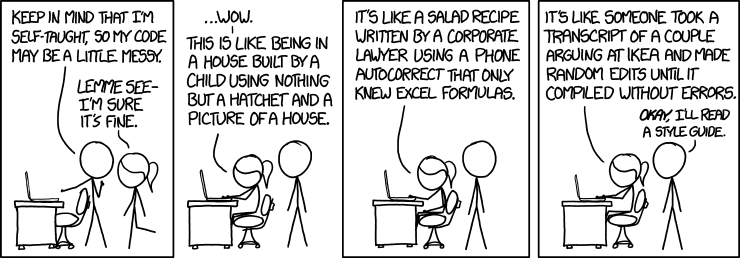
\includegraphics[width=\linewidth]{./gfx/xkcd-codeQuality}
\caption
	[Code Quality]
	{Code Quality. Quelle: \url{https://xkcd.com/1513/}}
\end{center}
\end{figure}
Immer wieder wird die Frage gestellt, welche Programmteile sinnvoll in Funktionen ausgelagert werden sollten und welche nicht. Während es dafür keine allgemeingültige Formel gibt, kann man zumindest einige Situationen aufführen, in denen es sich anbietet, Code in einer eigenen Funktion anzulegen.

Generell ist es sinnvoll, alle Arbeitsschritte, die eine gedankliche Einheit bilden, in einer Funktion zu verkapseln. Eine gedankliche Einheit ist etwa \enquote{Berechne den Wert einer Funktion} oder \enquote{Gib Text auf dem Bildschirm aus}.

Insbesondere sollte aller Code, den man mehrfach verwenden will in Funktionen stehen. Kopierter Code macht das Programm länger und damit schwieriger zu warten. Vor allem aber ergibt sich daraus eine Fehlerquelle, da Änderungen an einem kopierten Codeteil verlangen, auch alle anderen Stellen zu ändern, an denen diese Kopien auftauchen. Es ist leicht, diese Stellen zu vergessen und so inkonsistenten und fehlerhaften Code zu erhalten.

Schließlich kann es von Vorteil sein, selbst Codeblöcke in Funktionen zu setzen, die nur einmal aufgerufen werden. Ein Funktionsname sollte eindeutig beschreiben, welche Aufgabe die Funktion erfüllt. Ist dies gegeben, so kann der Ablauf eines Programms klarer im Code gelesen werden, ohne jedes Detail Zeile für Zeile nachvollziehen zu müssen. Sehen Sie sich dazu folgenden Code an:

\begin{codebox}[Beispiel: \texttt{main} eines Spiels]
\begin{minted}[linenos]{c}
/* ... #include-Zeilen stehen hier ... */

/* ... Funktionen stehen hier ... */

int main () {
  showTitleAnimation();

  int selectedMenuPoint = 0;
  do {
    showMenuScreen();
    selectedMenuPoint = askForMenuOption();
    performAction(selectedMenuPoint);
  } while(selectedMenuPoint);
}
\end{minted}
\end{codebox}

Hier wird vor Start des Spiels eine Animation gezeigt. Im Anschluss wird jeweils in Folge ein Menü\-bildschirm dargestellt, eine Usereingabe angenommen und dann dafür gesorgt, dass die Auswahl des Users ausgeführt wird. Dies wird solange durchgeführt, bis die Funktion \texttt{askForMenuOption} den Wert~\texttt{0} zurückgibt. Dies könnte (und sollte) \eg dann der Fall sein, wenn der User auswählt, das Spiel zu beenden.

Obwohl in diesem Beispiel nicht klar ist, wie die Animation im Detail aussieht, oder welche Menüpunkte angeboten werden, ist klar, wie das Programm organisiert ist. Neue Features können leicht eingefügt werden. Soll etwa eine Animation ausgeführt werden, sobald ein Menupunkt ausgewählt wurde, so kann nach Zeile 11 noch eine neue Funktion \texttt{showMenuAnimation(selectedMenuPoint)} eingefügt werden.

Funktionen können sich auch untereinander aufrufen, wie wir in Abschnitt \ref{sec:forwardDeclaration} gesehen haben. Dies \enquote{kostet} einigen Verwaltungsaufwand (um den wir als ProgrammiererInnen uns aber nicht explizit kümmern müssen). Der Compiler muss für jeden Aufruf einer Funktion mitspeichern, an welche Stelle bei Verlassen der aufgerufenen Funktion zurück gesprungen werden soll; außerdem müssen die Speicherbereiche für die einzelnen Funktionen angelegt und wieder frei gegeben werden. Bei geringer \emph{Aufruftiefe} (bis etwa 20 Aufruf-Ebenen) fällt dies nicht weiter ins Gewicht. Stärkere Verschachtelung macht Programme aber merklich langsamer. Natürlich ist es vor allem schwierig, eine Struktur mit so vielen Ebenen zu überblicken. Daher möchte ich Ihnen diesen Gedanken als einzige Beschränkung für die Sinnhaftigkeit von Funktionen mitgeben: halten Sie die Verschachtelung klein und übersichtlich. In Kapitel \ref{chp:recursion} werden wir diesen Gedanken nochmals aufgreifen.

\subsection{Rückgabe mehrerer Werte}
Eine Funktion kann nur entweder nichts (\mintinline{c}{void}) oder genau einen einzigen Wert zurückgeben. Es gibt aber Situationen, in denen dieselbe Funktion \emph{mehrere} Werte zugleich berechnen soll. Um dies zu ermöglichen stehen uns zwei Techniken zur Verfügung: Wir können ein \emph{Array} oder ein \mintinline{c}{struct} zurückgeben.

Arrays werden über Pointer verwaltet, daher muss der Rückgabetyp auch ein Pointer sein. (Tatsächlich gibt unsere Funktion also nur einen einzigen Wert zurück; dieser gibt dann aber eine Speicherstelle an, an der alle berechneten Werte zu finden sind.)

Sehen Sie sich folgendes Beispiel an, das ein Rezept für Obstsalat auf verschiedene Menschenmengen anpasst:

\begin{codebox}[Beispiel: Umrechnung eines Rezepts]
\begin{minted}[linenos]{c}
#include <stdio.h>
#include <stdlib.h>
// https://www.chefkoch.de/rezepte/654221166964999/Bunter-Obstsalat.html

double * fruitsaladForPersons(double persons) {
  double * reVal = malloc(8 * sizeof(*reVal));

  reVal[0] = persons/4.0 *   3;  // apples
  reVal[1] = persons/4.0 *   2;  // bananas
  reVal[2] = persons/4.0 *   2;  // peaches
  reVal[3] = persons/4.0 *   2;  // kiwis
  reVal[4] = persons/4.0 *   1;  // mangos
  reVal[5] = persons/4.0 *   1;  // oranges
  reVal[6] = persons/4.0 * 200;  // grams of grapes
  reVal[7] = persons/4.0 *  50;  // grams of walnuts

  return reVal;
}

int main () {
  double persons = 2;
  double * requirements = fruitsaladForPersons(persons);

  printf("Obstsalat für %1.0lf Personen:\n", persons);
  printf("\tÄpfel    : %5.1lf\n"  , requirements[0]);
  printf("\tBananen  : %5.1lf\n"  , requirements[1]);
  printf("\tPfirsiche: %5.1lf\n"  , requirements[2]);
  printf("\tKiwis    : %5.1lf\n"  , requirements[3]);
  printf("\tMangos   : %5.1lf\n"  , requirements[4]);
  printf("\tOrangen  : %5.1lf\n"  , requirements[5]);
  printf("\tTrauben  : %5.1lf g\n", requirements[6]);
  printf("\tWalnüsse : %5.1lf g\n", requirements[7]);

  free(requirements);
}
\end{minted}
\end{codebox}

\begin{cmdbox}[Ausführungsbeispiel: Umrechnung eines Rezepts]
\begin{minted}{text}
Obstsalat für 2 Personen:
        Äpfel    :   1.5
        Bananen  :   1.0
        Pfirsiche:   1.0
        Kiwis    :   1.0
        Mangos   :   0.5
        Orangen  :   0.5
        Trauben  : 100.0 g
        Walnüsse :  25.0 g
\end{minted}
\end{cmdbox}

Beachten Sie hier auch, dass der in Zeile 5 reservierte Speicherbereich wieder freigegeben werden muss. Dies geschieht in Zeile 35.

\mintinline{c}{struct}s werden in Kapitel \ref{chp:structs} besprochen.

\subsection{Speicherklasse \mintinline{c}{static}} \label{sec:staticVar}
Variablen sind immer nur in ihrem aktuellen Scope sichtbar, und werden \idR zerstört, sobald der aktuelle Scope verlassen wird. Manchmal soll aber der Wert einer Speicherstelle erhalten bleiben, selbst wenn die Ausführung den Scope verlässt, in dem die Variable definiert wurde. Bisher können wir dies nur lösen, indem wir die entsprechende Variable in einem Scope anlegen, das für die gesamte Lebensdauer des Programms existiert (also in der \texttt{main} oder als globale Variable), und einen Pointer auf diesen Wert \enquote{durchreichen}.

\begin{codebox}[Beispiel: Funktionsaufrufe mitzählen (1)]
\begin{minted}[linenos]{c}
#include <stdio.h>

void foobar(int * callCounter) {
  (*callCounter)++;
  printf("Aufruf #%d\n", *callCounter);
}

int main () {
  int calls = 0;

  foobar(&calls);
  foobar(&calls);
}
\end{minted}
\end{codebox}

\begin{cmdbox}[Ausführungsbeispiel: Funktionsaufrufe mitzählen (1)]
\begin{minted}{text}
Aufruf #1
Aufruf #2
\end{minted}
\end{cmdbox}

Dieser Code funktioniert zwar, ist aber fehleranfällig. Zunächst muss ein Anwender den Zweck von \texttt{calls} kennen, um die Funktion \texttt{foobar} richtig zu nutzen. Insbesondere darf \texttt{calls} nicht versehentlich geändert werden. Nicht zuletzt \enquote{belegt} diese Technik einen Variablennamen in der \texttt{main}.

Als Alternative dazu können Variablen in der Funkton \texttt{foobar} mit dem Schlüsselwort \mintinline{c}{static} deklariert werden. Auf diese Weise bleibt die Speicherstelle reserviert, \ie gespeicherte Werte erhalten, auch wenn die Funktion später wieder aufgerufen wird. Der Scope-Mechanismus hingegen wird nicht außer Kraft gesetzt. In Code sieht das dann so aus:

\begin{codebox}[Beispiel: Funktionsaufrufe mitzählen (2)]
\begin{minted}[linenos]{c}
#include <stdio.h>

void foobar() {
  static int callCounter = 0;
  callCounter++;
  printf("Aufruf #%d\n", callCounter);
}

int main () {
  foobar();
  foobar();
  // printf("%d\n", callCounter); -- unzulässig, falscher Scope
}
\end{minted}
\end{codebox}

Der Compiler legt \emph{ein einziges Mal} die Speicherstelle für \texttt{callCounter} an, selbst wenn (wie hier) die Funktion \texttt{foobar} mehrfach aufgerufen wird. Entsprechend findet auch die Wertzuweisung in Zeile 4 nur ein einziges Mal statt. Danach \enquote{erinnert} sich der Compiler an die bereits angelegte Speicherstelle sobald \texttt{foobar} \enquote{betreten} wird, \enquote{vergisst} aber diesen Variablennamen (nicht aber die Speicherstelle selbst) wieder, wenn die Funktion verlassen wird.

\section{Optimierung: \mintinline{c}{inline}} \label{sec:inline}
Bei einem Funktionsaufruf werden die Werte von Parametern kopiert.  Ebenso wird die Stelle gespeichert, von der weg gesprungen wurde, so dass beim Verlassen der Funktion die Ausführung nach dem Sprung-Befehl dort fortgesetzt werden kann. Dieses Kopieren und Speichern kostet Zeit. Bei häufig wiederkehrenden Aufrufen führt dies zu merklichen Performance-Einbrüchen.

Um dem entgegen zu wirken, können \emph{kurze} Funktionen als \mintinline{c}{inline} deklariert werden\footnote{Es gibt allerdings keine Garantie dafür, dass der Compiler die Funktion wirklich an entsprechende Stellen im einfügt. Es handelt sich also lediglich um einen Hinweis an den Compiler.}. Dies teilt dem Compiler mit, dass der Funktionskörper an der aufrufenden Stelle eingefügt werden sollte, statt einen normalen Sprung und Rücksprung durchzuführen. Ergebnis ist eine größere ausführbare Datei (da derselbe Code an mehreren Stellen eingefügt wird), der aber schneller läuft. Für die ProgrammiererInnen ergibt sich sonst kein Unterschied -- Funktionsaufruf sowie Scoping funktionieren wie bisher besprochen.

Um eine Funktion als \mintinline{c}{inline} zu deklarieren, schreibt man eine forward declaration und stellt dieser das Schlüsselwort \mintinline{c}{inline} voran:

\begin{codebox}[Syntax: \texttt{inline}-Funktion]
\begin{minted}{c}
inline Rückgabetyp Funktionsname (Parameterliste);
\end{minted}
\end{codebox}

\begin{codebox}[Beispiel: Maximum von zwei Ganzzahlen finden]
\begin{minted}[linenos]{c}
inline int max (int a, int b);
       int max (int a, int b) {return a > b   ?   a  :  b;}
\end{minted}
\end{codebox}

\section{Funktionszeiger} \label{sec:funcPtr}
Alle Objekte mit denen wir arbeiten müssen im Speicher abgelegt werden. Sie haben daher notwendigerweise auch eine Adresse. Dies umfasst einzelne Zahlen, Gruppen von Zahlen (Arrays) und eben auch Programmcode. Bei der Ausführung eines Programms wird dieses zunächst in den Arbeitsspeicher kopiert, und dann die Maschinencode-Anweisungen ausgeführt, die in der Datei vermerkt waren. Wir können die Adressen von bestimmten Programmteilen ausfindig machen und mit der Ausführung an diese Adressen springen. Zu diesem Zweck existiert das Konzept von \texttt{Funktionszeigern}, also Pointer auf Funktionen.

Funktionszeiger sind wie alle Pointer Variablen, die zunächst deklariert werden müssen. Diese Deklaration enthält alle Informationen der Funktionssignatur, also Rückgabewert der Funktion und Parameterliste. Dies drückt sich in der folgenden (leider etwas unhandlichen Syntax) aus:
\begin{codebox}[Syntax: Deklaration Funktionszeiger]
\begin{minted}{c}
Rückgabetyp (*Variablenname) (Parameterliste);
\end{minted}
\end{codebox}

Solchen Variablen kann nun die Adresse einer beliebigen Funktion (mit passender Signatur) zugewiesen werden. Dies geschieht \emph{ohne} jegliche Operatoren, einfach über den Funktionsnamen:

\begin{codebox}[Beispiel: Funktionszeiger (1)]
\begin{minted}[linenos]{c}
#include <stdio.h>

void foo() {
  printf("blerb.\n");
}

int main () {
  void (*funcPtr)() = foo;
}
\end{minted}
\end{codebox}

Der Codeabschnitt, auf den dieser Funktionspointer zeigt, kann nun mit dem neuen Symbol \texttt{funcPtr} aufgerufen werden, ganz als würde man direkt mit \texttt{foo} arbeiten:

\begin{codebox}[Beispiel: Funktionszeiger (2)]
\begin{minted}[linenos]{c}
#include <stdio.h>

void foo() {
  printf("blerb.\n");
}

int main () {
  void (*funcPtr)() = foo;
\end{minted}
\end{codebox}
%
\begin{codebox}[]
\begin{minted}[linenos]{c}
  printf("direkt : ");
  foo();

  printf("funcPtr: ");
  funcPtr();
}
\end{minted}
\end{codebox}

\begin{cmdbox}[Ausführungsbeispiel: Funktionszeiger (2)]
\begin{minted}{text}
direkt : blerb.
funcPtr: blerb.
\end{minted}
\end{cmdbox}

\begin{hintbox}
Der Name einer Funktion beschreibt selbst einen Funktionszeiger! Der Aufruf einer Funktion ist eine \emph{Operation}, vergleichbar mit dem Dereferenzieren (Operator \texttt{*}). Daher müssen auch Funktionen, die keine Parameter erwarten, mit leeren Klammern () aufgerufen werden.
\end{hintbox}

Der Zweck dieser Technik ist, das Verhalten anderer Funktionen vom Ergebnis anderer Berechnungen abhängig zu machen, ohne sich dabei auf die Art der Berechnung festzulegen.

Als Beispiel sei die Funktion \texttt{qsort}\footnote{Der Sortieralgorithmus \emph{quicksort}, der dieser Funktion zugrunde liegt, wird in der Vorlesung \emph{Algorithmen und Datenstrukturen} an der Universität Regensburg genauer besprochen.} genannt (definiert in \texttt{stdlib.h}). Diese Funktion kann Arrays beliebigen Typs nach beliebigen Kriterien sortieren. Die Sortier-Kriterien werden in Form einer Funktion \texttt{comp} beschrieben, die zwei Werte \texttt{a} und \texttt{b} miteinander vergleicht. (Hier verwende ich den Namen \texttt{comp}, um den folgenden Abschnitt leichter lesbar zu halten; die Vergleichsfunktion darf in der Anwendung aber einen beliebigen Namen haben.)

Da Arrays \emph{beliebigen} Typs sortiert werden, können an \texttt{comp} nicht die \emph{Werte} \texttt{a} und \texttt{b} übergeben werden, sondern nur ihre \emph{Adressen} \texttt{\&a} und \texttt{\&b}.

Wenn \texttt{a} \emph{vor} \texttt{b} in der sortierten Liste auftauchen soll, soll der Rückgabewert von \texttt{comp(\&a, \&b)} gleich \texttt{-1} sein. Falls dagegen \texttt{b} vor \texttt{a} sortiert werden soll, so muss \texttt{+1} zurückgegeben werden. Schließlich wird \texttt{comp} den Wert \texttt{0} zurückgeben, wenn \texttt{a} und \texttt{b} gleichwertig sind. (\emph{Gleichwertig} bedeutet in diesem Kontext nicht zwingend \emph{gleich}. Wir könnten zum Beispiel Zahlen nach ihrer Quersumme sortieren. Für diese Sortierung sind die Zahlen \texttt{19} und \texttt{91} dann gleichwertig, nicht aber gleich.)

Die \href{https://en.cppreference.com/w/c/algorithm/qsort}{cpp-Referenz} teilt uns die Signatur der Funktion \texttt{qsort} mit:

\begin{codebox}[Prototyp der Funktion \texttt{qsort}]
\begin{minted}{c}
void qsort( void * ptr, size_t count, size_t size,
            int (*comp)(const void *, const void *) );
\end{minted}
\end{codebox}

Betrachten wir die einzelnen Parameter:
\begin{itemize}
\item Der erste Parameter \texttt{ptr} ist ein Pointer auf ein beliebiges Array und daher vom Typ
		\mintinline{c}{void *}.
\item Mit \texttt{count} wird die Zahl der Elemente des Arrays beschrieben. (Der Typ
		\mintinline{c}{size_t} ist ein Alias (ein alternativer Name) für \mintinline{c}{unsigned int}.)
\item Der Wert \texttt{size} beschreibt den Speicherbedarf \emph{eines} Elements des Arrays. Wir
		brauchen diese Information, da \texttt{qsort} \ua für \mintinline{c}{int}-,
		\mintinline{c}{double}- oder \mintinline{c}{char}-Arrays funktionieren soll, die allesamt
		unterschiedlichen Speicherbedarf haben.
\item Die letzte Zeile schließlich benennt den Parameter \texttt{comp}, der eine Vergleichsfunktion
		benennt. Diese Funktion wird einen \mintinline{c}{int} zurück geben, und nimmt zwei
		\mintinline{c}{const void *} als Argumente an. Dabei bedeutet \mintinline{c}{const} wieder, dass
		\texttt{comp} die Werte von \texttt{a} und \texttt{b} nur lesen, nicht aber verändern wird.
		Der Modifier \mintinline{c}{const} gehört zum Datentyp und muss daher auch in unserer Funktions-
		Signatur auftauchen. Wieder gilt: Da der Datentyp von \texttt{a} und \texttt{b} beliebig ist,
		können nur \mintinline{c}{void *} übergeben werden.
\end{itemize}

Mit diesen Informationen können wir das (leicht abgewandelte) Beispiel von der \href{https://en.cppreference.com/w/c/algorithm/qsort}{cpp-Referenz} verstehen:

\begin{codebox}[Beispiel: \texttt{qsort} mit zwei Sortiermethoden]
\begin{minted}[linenos]{c}
#include <stdio.h>
#include <stdlib.h>

int comp_ascending(const void* a, const void* b) {
    int arg1 = *(const int *) a;
    int arg2 = *(const int *) b;

    if (arg1 < arg2) return -1;
    if (arg1 > arg2) return  1;
    return 0;
}

int comp_descending(const void* a, const void* b) {
    return -comp_ascending(a, b);
}

int main(void) {
    int ints[] = { -2, 99, 0, -743, 2, 4 };
    int size = sizeof(ints) / sizeof(*ints);

    printf("Aufsteigende Sortierung:\n");
    qsort(ints, size, sizeof(int), comp_ascending);

    for (int i = 0; i < size; i++) {
        printf("%d ", ints[i]);
    }
    printf("\n");

    printf("Absteigende Sortierung:\n");
    qsort(ints, size, sizeof(int), comp_descending);

    for (int i = 0; i < size; i++) {
        printf("%d ", ints[i]);
    }
    printf("\n");
}
\end{minted}
\end{codebox}

\begin{cmdbox}[Ausführungsbeispiel: \texttt{qsort} mit zwei Sortiermethoden]
\begin{minted}{text}
Aufsteigende Sortierung:
-743 -2 0 2 4 99
Absteigende Sortierung:
99 4 2 0 -2 -743
\end{minted}
\end{cmdbox}

Obwohl die Funktion \texttt{qsort} nur einmal programmiert wurde, kann sie mit diesen Techniken also \emph{generisch} benutzt werden, \ie sie ist für viele verschiedene Zwecke einsetzbar, die bei der Erstellung von \texttt{qsort} noch nicht einmal vorgesehen waren.

	\chapter{Speicher-Strukturen} \label{chp:structs}
\epigraph{There are two ways of constructing a software design: One way is to make it so simple that there are obviously no deficiencies, and the other way is to make it so complicated that there are no obvious deficiencies. The first method is far more difficult.}
{C.A.R. Hoare}

Werte im Speicher bilden oft funktionelle Einheiten. In einem Jump'n'Run-Game gehören beispielsweise die x- und y-Koordinate, Blickrichtung sowie die Lebenspunkte der Spielfigur \enquote{zusammen}. Es bietet sich an, Aufgaben wie die Animation beim Laufen, die Überprüfung auf Kollision mit anderen Spielelementen und ähnliches jeweils in Funktionen auszulagern. Diesen Funktionen müssen dann aber jeweils alle genannten Daten als Parameter übergeben werden. Dies kann schnell lästig werden und bietet zusätzlich eine Fehlerquelle, da die Parameter in der richtigen Reihenfolge übergeben werden müssen. An dieser Stelle wollen wir Methoden betrachten, die solche thematischen Einheiten zu kompakten Blöcken zusammen zu fassen.

\section{Sammlungen von Werten: \mintinline{c}{struct}s}
Ein \mintinline{c}{struct} ist ein \emph{selbstdefinierter Datentyp}, in dem mehrere Datensätze zu einem Block zusammengefasst werden. Man kann sich eine \mintinline{c}{struct} also wie eine Sammlung von Tabellenköpfen vorstellen. \mintinline{c}{struct}s haben einen Typen-Namen, sowie für jede Zeile der Tabelle einen Datentyp und einen Feldnamen.

Eine \mintinline{c}{struct} wird folgendermaßen deklariert:
\begin{codebox}[Syntax: Deklaration einer \texttt{struct}]
\begin{minted}{c}
struct Name {
  Datentyp Feldname1;
  Datentyp Feldname2;
  ...
};
\end{minted}
\end{codebox}

Wie üblich ist \texttt{Name} dabei eine alphanumerische Zeichenkette aus bis zu 40 Zeichen, die einen eindeutigen Namen beschreibt, \ie die nicht schon eine Variable im aktuellen Scope oder eine Funktion benennt.

\texttt{Datentyp} ist ein beliebiger Datentyp wie \mintinline{c}{int}, inclusive Pointern oder anderen \mintinline{c}{struct}s.

Die \texttt{Feldname}n sind alphanumerische Zeichenketten von bis zu 40 Zeichen Länge, die jedoch \emph{nicht} global eindeutig sein müssen: eine \mintinline{c}{struct} öffnet ihren eigenen Scope (vgl. die \{geschweiften Klammern\}, in die die Scope-Felder eingeschlossen sind).

Grundsätzlich kann eine \mintinline{c}{struct} an jeder Stelle im Programm angelegt werden; sie ist dann wie gewohnt nur für den aktuellen Scope gültig. Meist wird die Definition einer \mintinline{c}{struct} im gesamten Programm gebraucht; man setzt sie daher üblicherweise global, also vor/außerhalb der \mintinline{c}{main}.

Mit dieser Defintion einer \mintinline{c}{struct} kann man nun Variablen dieses Typs anlegen. Eine Variable eines solchen Typs kann man sich als Spalte einer solchen Tabelle vorstellen. Eine solche Variable wird in einem sinnvollen Scope (\eg in der \texttt{main}) deklariert mit der Syntax:

\begin{codebox}[Syntax: Deklaration einer \texttt{struct}]
\begin{minted}{c}
struct Name Variablenname;
\end{minted}
\end{codebox}

\begin{tcbraster}[raster columns=2,
                  raster equal height,
                  nobeforeafter,
                  raster column skip=0.1cm]
\begin{codebox}[Beispiel: Deklaration einer \texttt{struct}]
\begin{minted}[linenos]{c}
struct Karteieintrag {
  char vorname[50];
  char nachname[50];
  int  geburtsjahr;
  int  geburtsmonat;
  int  geburtstag;
};

int main () {
   struct Karteieintrag Cessi, Chami;
}
\end{minted}
\end{codebox}%
%
\begin{tcolorbox}[title=Visualisierung: Sammlung Tabellenköfpe]
\begin{tabular}{|l|l|l|}
\toprule[1pt]
\emph{Tabellenkopf}		& \texttt{Cessi}	& \texttt{Chami}	\tabcrlf
\texttt{vorname}			& Ce				& Lisl			\tabcrlf
\texttt{nachname}		& Saurus 		& Kohlenstoff	\tabcrlf
\texttt{geburtsjahr}		& 1897			& 1996			\tabcrlf
\texttt{geburtsmonat}	& 9				& 9				\tabcrlf
\texttt{geburtstag}		& 30				& 26				\\
\bottomrule[1pt]
\end{tabular}
\vfill
\end{tcolorbox}
\end{tcbraster}

% include gfx: Rows with type names; 

\subsection{Direkter Zugriff auf \mintinline{c}{struct}-Elemente}
Im obigen Beispiel haben wir die \mintinline{c}{struct} definiert und Variablen des Typs \mintinline{c}{struct Karteieintrag} deklariert. Um nun die einzelnen Felder anzusprechen (\ie die Tabellen-Elemente zu lesen und zu schreiben) bedienen wir uns der Syntax \texttt{Variable.Feldname}. Achten hier auf die Unterscheidung zwischen \emph{Datentyp} (\eg \mintinline{c}{struct Karteieintrag}), \emph{Variable} (\eg \texttt{Cessi}) und \emph{Feldname} (\eg \texttt{vorname}).

\begin{codebox}[Beispiel: Deklaration einer \texttt{struct} und Schreiben in eine \texttt{struct}-Variable]
\begin{minted}[linenos]{c}
#include <string.h>

struct Karteieintrag {                 // Deklaration Datentyp
  char vorname[50];                    // Deklaration Feldelemente
  char nachname[50];
  int  geburtsjahr;
  int  geburtsmonat;
  int  geburtstag;
};

int main () {
  struct Karteieintrag Cessi, Chami;   // Deklaration Variablen
  
  strcpy(Cessi.vorname,  "Ce");        // Zugriffe auf Feldelemente in 'Cessi'
  strcpy(Cessi.nachname, "Saurus");
  Cessi.geburtsjahr  = 1897;
  Cessi.geburtsmonat =    9;
  Cessi.geburtstag   =   30;
\end{minted}
\end{codebox}
\begin{codebox}[]
\begin{minted}[linenos, firstnumber=last]{c}
  strcpy(Chami.vorname,  "Lisl");      // Zugriffe auf Feldelemente in 'Chami'
  strcpy(Chami.nachname, "Kohlenstoff");
  Chami.geburtsjahr  = 1996;
  Chami.geburtsmonat =    9;
  Chami.geburtstag   =   26;
}
\end{minted}
\end{codebox}

Anstatt nun also mit zwei mal fünf getrennten Variablen hantieren zu müssen, können wir nun fünf Werte \enquote{als Paket} behandeln; ein solches Paket darf beispielsweise als Parameter einer Funktion übergeben. Vergleichen Sie die beiden folgenden Funktionen sowie ihre Aufrufe:

\begin{codebox}[Beispiel: Vergleich: Funktion mit \texttt{struct}-Parameter und getrennte Variablen]
\begin{minted}[linenos]{c}
#include <stdio.h>
#include <string.h>

struct Karteieintrag {
  char vorname[50];
  char nachname[50];
  int  geburtsjahr;
  int  geburtsmonat;
  int  geburtstag;
};

void KarteiZeigenGetrennt (
  char vorname[50],
  char nachname[50],
  int  geburtsjahr,
  int  geburtsmonat,
  int  geburtstag
) {
  printf("Vorname:\t%s\n", vorname);
  printf("Nachname:\t%s\n", nachname);
  printf("Geburtstag:\t%04d-%02d-%02d\n",
    geburtsjahr, geburtsmonat, geburtstag
  );
}

void KarteiZeigenStruct (struct Karteieintrag person) {
  printf("Vorname:\t%s\n", person.vorname);
  printf("Nachname:\t%s\n", person.nachname);
  printf("Geburtstag:\t%04d-%02d-%02d\n",
    person.geburtsjahr, person.geburtsmonat, person.geburtstag
  );
}

int main () {
  struct Karteieintrag Cessi, Chami;
  
  /* Eintragen von Werten in Variablen 'Cessi', 'Chami' */
\end{minted}
\end{codebox}
\begin{codebox}[]
\begin{minted}[linenos, firstnumber=last]{c}
  KarteiZeigenGetrennt(
    Cessi.vorname,
    Cessi.nachname,
    Cessi.geburtsjahr,
    Cessi.geburtsmonat,
    Cessi.geburtstag
  );
  
  printf("\n");
  
  KarteiZeigenStruct(Chami); 
}
\end{minted}
\end{codebox}

\begin{cmdbox}[Ausgabebeispiel: Vergleich: Funktion mit \texttt{struct}-Parameter und getrennte Variablen]
\begin{minted}{text}
Vorname:        Ce
Nachname:       Saurus
Geburtstag:     1897-09-30

Vorname:        Lisl
Nachname:       Kohlenstoff
Geburtstag:     1996-09-26
\end{minted}
\end{cmdbox}

Beide Varianten erzeugen eine Ausgabe derselben Form. Bei \texttt{KarteiZeigenGetrennt} müssen jedoch alle fünf Werte im Aufruf getrennt aufgeführt werden (Zeilen 38-44), und erhalten in der Funktionssignatur einen eigenen Eintrag (Zeilen 12-18). Bei der \mintinline{c}{struct}-Version \texttt{KarteiZeigenStruct} dagegen kann der komplette Datensatz \enquote{als Einheit} übergeben werden (Zeile 48). Entsprechend kürzer fällt auch die Funktionssignatur aus (Zeile 26): Hier wird nur eine einzelne Variable \texttt{person} vom Typ \mintinline{c}{struct Karteieintrag} entgegengenommen.

Auch \mintinline{c}{struct}s können ineinander verschachtelt werden:
\begin{codebox}[Beispiel: Verschachtelte Structs]
\begin{minted}[linenos]{c}
struct Datum {
  int  jahr;
  int  monat;
  int  tag;
};

struct Karteieintrag {
  char         vorname[50];
  char         nachname[50];
  struct Datum geburtstag;
};

int main () {
  struct Karteieintrag Tiny;
  Tiny.geburtstag.jahr  = 1994;
  Tiny.geburtstag.monat =    2;
  Tiny.geburtstag.tag   =    3;
}
\end{minted}
\end{codebox}

\subsection{Aliase für Datentypen: \mintinline{c}{typedef}} \label{sec:typedef}
\mintinline{c}{struct}s erlauben zwar bedutend übersichtlichere Strukturen; es wird aber bald lästig, widerholt das Schlüsselwort \mintinline{c}{struct} selbst zu tippen. Aus diesem Grund wird die Deklaration von \mintinline{c}{struct}s häufig mit \mintinline{c}{typedef} verbunden.

\mintinline{c}{typedef} wird benutzt, um zu bestehenden Namen von Datentypen alternative Namen zu definieren (sogenannte \emph{Aliase}). Dies folgt der Syntax:

\begin{codebox}[Syntax: Deklaration einer \texttt{struct}]
\begin{minted}{c}
typedef BezeichnerOriginaltyp Alias;
\end{minted}
\end{codebox}

Sobald auf diese Weise ein \texttt{Alias} definiert ist, kann dieser an jeder Stelle im Code benutzt werden und ersetzt so den gesamten Ausdruck \texttt{BezeichnerOriginaltyp}.

\begin{codebox}[Beispiel: \texttt{typedef} und \texttt{struct}]
\begin{minted}[linenos]{c}
struct Karteieintrag_struct {
  char vorname[50];
  char nachname[50];
  int  geburtsjahr;
  int  geburtsmonat;
  int  geburtstag;
};

typedef struct Karteieintrag_struct Karteieintrag;

int main () {
   Karteieintrag Cessi, Chami;
}
\end{minted}
\end{codebox}

Typedef kann auch für vordefinierte Datentypen benutzt werden, die häufig getippt werden müssen:
\begin{codebox}[Beispiel: \texttt{typedef} und lange Standard-Typen]
\begin{minted}[linenos]{c}
typedef unsigned long long int bignum;
bignum globalvar = 999999999999999999;
\end{minted}
\end{codebox}

Die Definition des Alias \texttt{Karteieintrag} für \mintinline{c}{struct Karteieintrag_struct} erspart in Zeile 12 die Wiederholung des Schlüsselworts \mintinline{c}{struct}; insbesondere gilt das auch für alle weiteren Referenzen auf den Datentyp wie etwa in der Signatur von Funktionen. Neben der Typenbezeichnunt \texttt{Karteieintrag} kann aber auch weiterhin \mintinline{c}{struct Karteieintrag_struct} als Synonym verwendet werden.

Noch kompakter und bequemer wird dies bei der Verwendung von \emph{anonymen \mintinline{c}{struct}s}, also \mintinline{c}{struct}s ohne eigenen Namen. Hier kann die Auflistung der Felder direkt in den \mintinline{c}{typedef}-Befehl mit aufgenommen werden:

\begin{codebox}[Beispiel: \texttt{typedef} und \texttt{struct}]
\begin{minted}[linenos]{c}
typedef struct {
  char vorname[50];
  char nachname[50];
  int  geburtsjahr;
  int  geburtsmonat;
  int  geburtstag;
} Karteieintrag;

int main () {
   Karteieintrag Cessi, Chami;
}
\end{minted}
\end{codebox}

Schließlich ist es auch möglich, im selben Zuge \emph{abgeleitete} Typen zu definieren, \eg einen Pointer auf die soeben definierte \mintinline{c}{struct}:

\begin{codebox}[Beispiel: \texttt{typedef} und \texttt{struct} mit abgeleitetem Typ]
\begin{minted}[linenos]{c}
typedef struct {
  char vorname[50];
  char nachname[50];
  int  geburtsjahr;
  int  geburtsmonat;
  int  geburtstag;
} Karteieintrag, * pKarteieintrag;

int main () {
    Karteieintrag   Cessi;
   pKarteieintrag   CessiRef1 = &Cessi;
    Karteieintrag * CessiRef2 = &Cessi;
}
\end{minted}
\end{codebox}

Durch das \texttt{*} in Zeile 7 wird ausgedrückt, dass das folgende Symbol \texttt{pKarteieintrag} einen Pointer auf die definierte Struktur beschreibt. Folglich wird in Zeile 11 mit \texttt{CessiRef1} eine Variable definiert, die ein Pointer auf \texttt{Karteieintrag} ist. Daneben existiert auch die bereits bekannte Form aus Zeile 12. Die Variablen \texttt{CessiRef1} und \texttt{CessiRef2} haben also denselben Datentyp.

\begin{hintbox}[Sinn und Unsinn von \texttt{typedef}s]
Die Möglichkeit, mit \mintinline{c}{typedef} kürzere Aliase für unhandliche Ausdrücke einzuführen birgt die Gefahr, sich in einem undurchsichtigen Gewirr von Definitionen zu verstricken. Gerade wenn von \mintinline{c}{typedef}s noch andere Typen abgeleitet werden, ist es oft schwer, die \enquote{Verwandtschaftsbeziehungen} noch nachzuvollziehen und sinnvollen Code zu schreiben.

Nach meiner Erfahrung gibt es zwei Situationen, in denen \mintinline{c}{typedef} die Arbeit in C tatsächlich leichter macht:
\begin{itemize}
\item \mintinline{c}{struct}s sowie Pointer auf \mintinline{c}{struct}s, so wie oben gezeigt
\item Funktionszeiger, wie wir sie in Abschnitt \ref{sec:funcPtr} kennengelernt haben.
Die reine Umdefinition bestehender Typennamen dagegen sollte eher vermieden werden.
\end{itemize}
\end{hintbox}

\begin{hintbox}[]
Im Kontext von Funktionszeigern macht die Verwendung von \mintinline{c}{typedef} den Code nicht nur kürzer, sondern bedeutend intuitiver lesbar (sofern man sprechende Typennamen definiert). Sehen Sie folgendes Beispiel an:

\begin{codebox}[\texttt{typedef} und Funktionszeiger]
\begin{minted}{c}
typedef int (*funcPtr_comp) (const void *, const void *);

/* Originaldefintion wie von der cpp-Referenz
 * void qsort( void * ptr, size_t count, size_t size,
 *             int (*comp)(const void *, const void *) );
 */
void qsort (void * ptr, size_t count, size_t size, 
            funcPtr_comp comp);
\end{minted}
\end{codebox}
Die Originaldefinition erlaubt zwar, direkt Rückgabetyp und Typ der Parameter zu entnehmen; es ist aber schwierig, hier auf einen Blick zu erfassen, welches der Name des Parameters ist, und was zur Beschreibung des Typs gehört. In der zweiten Version wird vorausgesetzt, dass der/die ProgrammiererIn die Signatur von \texttt{comp} kennt; dafür wird die Signatur von \texttt{qsort} übersichtlich und entspricht eher einer menschlichen Gedankeneinheit. Die Meinungen hierzu gehen bisweilen aber weit auseinander.
\end{hintbox}

\mintinline{c}{struct}s können auch Pointer auf Instanzen desselben Typs enthalten:
\begin{codebox}[Beispiel: \texttt{struct} mit Referenz auf Instanz gleichen Typs]
\begin{minted}[linenos]{c}
struct linkedList{
  double              content;
  struct linkedList * next;
};
\end{minted}
\end{codebox}

Während das Symbol \mintinline{c}{struct linkedList} schon \enquote{in der Definition der \mintinline{c}{struct}} zur Verfügung steht, sind mit \mintinline{c}{typdef} definierte Symbole erst \emph{nach Abschluss} des Befehls verwendbar:

\begin{warnbox}[Beispiel: \texttt{typedef} und \texttt{struct} mit Referenz auf Instanz gleichen Typs (fehlerhaft), leftupper=7mm]
\begin{minted}[linenos]{c}
typedef struct {
  double       content;
  // linkedList * next;   // Fehler: linkedList noch nicht definiert
} linkedList;
\end{minted}
\end{warnbox}

Um für solche Strukturen dennoch den Komfort von \mintinline{c}{typedef} nutzen zu können, arbeitet man hier mit \emph{benannten \mintinline{c}{struct}s} (im Gegensatz zu \emph{anonymen \mintinline{c}{struct}s}):

\begin{codebox}[Beispiel: \texttt{typedef} und \texttt{struct} mit Referenz auf Instanz gleichen Typs (korrekt)]
\begin{minted}[linenos]{c}
typedef struct LL_struct {
  double             content;
  struct LL_struct * next;   // okay: struct LL_struct kann aufgelöst werden
} linkedList;                // Symbol linkedList steht ab hier zur Verfügung.
\end{minted}
\end{codebox}

In Kapitel \ref{chp:linkedlist} werden wir uns ausführlicher mit solchen Strukturen beschäftigen.

\subsection{\mintinline{c}{struct}s und Pointer}
Wie Sie bereits festgestellt haben, müssen wir in C häufig mit Pointern arbeiten. Im vorigen Abschnitt wurden bereits Pointer auf \mintinline{c}{struct}s angesprochen. Dazu sei hier zuerst ein Syntaxelement vorgestellt, und weiter einige Beispiele besprochen:

\subsubsection{Kombinierter Pointer-Feldzugriffs-Operator}
Haben wir einen Pointer auf eine \mintinline{c}{struct}, so muss für einen Feldzugriff der Pointer zuerst dereferenziert (Operator \texttt{*}) werden und anschließend das angesprochene Feld über den Feldzugriffoperator (\texttt{.}) ausgewählt werden. Da der Feldzugriffsoperator eine höhere Präzedenz hat als die Dereferenzierung (\ie \texttt{.} wird vor \texttt{*} ausgewertet; siehe Tabelle \ref{tab:OperatorPrecedence}), muss mit Klammern gearbeitet werden:

\begin{codebox}[Beispiel: Dereferenzierung und Feldzugriff]
\begin{minted}[linenos]{c}
/* Definition von Karteieintrag und pKarteieintrag wie im vorigen Kapitel */
int main () {
   Karteieintrag        Tiny;
  pKarteieintrag ptr = &Tiny;
  
  printf("Jahr: %4d\n", (*ptr).geburtsjahr);
}
\end{minted}
\end{codebox}

Diese umständliche Form kann durch den kombinierten \emph{Pointer-Feldzugriffs-Operator} \texttt{->} ersetzt werden:

\begin{codebox}[Beispiel: kombinierter Operator]
\begin{minted}[linenos]{c}
/* Definition von Karteieintrag und pKarteieintrag wie im vorigen Kapitel */
int main () {
   Karteieintrag        Tiny;
  pKarteieintrag ptr = &Tiny;
  
  printf("Jahr: %4d\n", ptr->geburtsjahr);
}
\end{minted}
\end{codebox}

\subsubsection{Pointer als Feldelemente}
Selbstverständlich können auch die Feldelemente einer \mintinline{c}{struct} selbst Pointer enthalten. In den obigen Beispielen etwa sind \texttt{vorname} und \texttt{nachname} \mintinline{c}{char}-Arrays und damit Pointer. Der Dereferenzierungs-Operator \texttt{*} wirkt in diesem Fall auf das Feldelement:
\begin{codebox}[Beispiel: Zugriff auf Pointer-Feldelemente (1)]
\begin{minted}[linenos]{c}
/* Definition von Karteieintrag und pKarteieintrag wie im vorigen Kapitel */
int main () {
  Karteieintrag Tiny;
  
  printf("Erster Buchstabe von Tinys Vornamen: %c\n", *Tiny.vorname);
}
\end{minted}
\end{codebox}

Ebenso verhält es sich mit dem Array-Index-Zugriffsoperator \texttt{[]}:
\begin{codebox}[Beispiel: Zugriff auf Pointer-Feldelemente (2)]
\begin{minted}[linenos]{c}
/* Definition von Karteieintrag und pKarteieintrag wie im vorigen Kapitel */
int main () {
  Karteieintrag        Tiny;
  
  printf("Erster Buchstabe von Tinys Vornamen: %c\n", Tiny.vorname[0]);
}
\end{minted}
\end{codebox}

\subsubsection{Pointer in Basis-Variable und in den Feldelementen}
Ist die Variable, über die die \mintinline{c}{struct} angesprochen wird, selbst eine Pointer-Variable, so wird der kombinierte Pointer-Feldzugriffs-Operator \texttt{->} zuerst aufgelöst; anschließend wirken \texttt{*} bzw \texttt{[]}:

\begin{codebox}[Beispiel: kombinierter Operator und Pointer-Feldelemente]
\begin{minted}[linenos]{c}
/* Definition von Karteieintrag und pKarteieintrag wie im vorigen Kapitel */
int main () {
   Karteieintrag        Tiny;
  pKarteieintrag ptr = &Tiny;
  
  printf("Erster Buchstabe von Tinys Vornamen: %c\n", *ptr->vorname   );
  printf("Erster Buchstabe von Tinys Vornamen: %c\n",  ptr->vorname[0]);
}
\end{minted}
\end{codebox}

Siehe hierzu auch Tabelle \ref{tab:OperatorPrecedence}.

\subsubsection{Arrays von Structs}
Man kann auch \emph{Arrays von \mintinline{c}{struct}s} anlegen. In diesem Fall setzt man den Array-Zugriffsoperator \texttt{[]} an die Array-Variable. Unabhängig davon können weiter Operationen auf Array-Feldelemente durchgeführt werden:

\begin{codebox}[Beispiel: Array von \texttt{struct}s]
\begin{minted}[linenos]{c}
typedef struct {
  char vorname[50];
  char nachname[50];
  int  geburtsjahr;
  int  geburtsmonat;
  int  geburtstag;
} Karteieintrag, * pKarteieintrag;
\end{minted}
\end{codebox}
%
\begin{codebox}[]
\begin{minted}[linenos, firstnumber=last]{c}
int main () {
  Karteieintrag listeGeburtstage[3];

  strcpy(listeGeburtstage[0].vorname,  "Ce");
  strcpy(listeGeburtstage[0].nachname, "Saurus");
  listeGeburtstage[0].geburtsjahr  = 1897;
  listeGeburtstage[0].geburtsmonat =    9;
  listeGeburtstage[0].geburtstag   =   30;
  
  strcpy(listeGeburtstage[1].vorname,  "Lisl");
  strcpy(listeGeburtstage[1].nachname, "Kohlenstoff");
  listeGeburtstage[1].geburtsjahr  = 1996;
  listeGeburtstage[1].geburtsmonat =    9;
  listeGeburtstage[1].geburtstag   =   26;
  
  strcpy(listeGeburtstage[2].vorname,  "Tiny");
  strcpy(listeGeburtstage[2].nachname, "Mürrisch");
  listeGeburtstage[2].geburtsjahr  = 1994;
  listeGeburtstage[2].geburtsmonat =    2;
  listeGeburtstage[2].geburtstag   =    3;
    
  printf("Erster Buchstabe Vorname 3: %c\n", *listeGeburtstage[2].vorname    );
  printf("Erster Buchstabe Vorname 3: %c\n",  listeGeburtstage[2]->vorname[0]);
}
\end{minted}
\end{codebox}

Machen Sie sich hier nochmal die Bedeutung der einzelnen Symbole klar:
\begin{itemize}
\item \texttt{Karteieintrag} ist ein \emph{Datentyp} und beschreibt nur die Struktur einer Variable; das
	Symbol selbst beschreibt aber keine Werte.
\item \texttt{pKarteieintrag} ist ebenfalls ein \emph{Datentyp}. Er beschreibt aber keine 
	\mintinline{c}{struct}, sondern einen \emph{Pointer} darauf, \ie die Information, wo im Speicher die
	tatsächliche Instanz der \mintinline{c}{struct} zu finden ist. Verbunden mit dieser Adresse ist die
	Information,  welche Art von Werten an der angegebenen Speicherstelle zu finden sind -- eben die 
	\mintinline{c}{struct} \texttt{Karteieintrag}.
\item \texttt{geburtstag} ist ein Element der \mintinline{c}{struct Karteieintrag}, und damit ohne
	Kontext ein nicht deklariertes Symbol. Nur in Verwendung mit Instanzen von \texttt{Karteieintrag}
	kann dieses Symbol gebraucht werden.
\item \texttt{listeGeburtstage} ist ein Array vom Typ \texttt{Karteieintrag} und damit eine Variable vom
	Typ \texttt{pKarteieintrag}. In dieser Variablen ist nur eine Zahl gespeichert, die die Adresse des 
	ersten Elements des Arrays im Speicher angibt.
\item \texttt{listeGeburtstage[0]} ist nun tatsächlich ein Objekt vom Typ \texttt{Karteieintrag}, \ie
	eine Sammlung von fünf Variablen. Man spricht auch von einer \emph{Instanz} von
	\texttt{Karteieintrag}. Es handelt sich um das erste Element der Liste. Dieser Ausdruck kann \eg an
	Funktionen übergeben werden, die als Argument ein Objekt vom Typ \texttt{Karteieintrag} erwarten 
	(wie im vorigen \emph{Beispiel: Vergleich: Funktion mit \texttt{struct}-Parameter und getrennte
	 Variablen} die Funktion \texttt{KarteiZeigenStruct}.)
\item \texttt{listeGeburtstage[1].geburtsjahr} ist ein \mintinline{c}{int}-Wert. Er gehört zu der
	Instanz 	\texttt{listeGeburtstage[1]}, also zur zweiten Instanz des Typs \texttt{Karteieintrag} im
	Array.
\item \texttt{listeGeburtstage[2].vorname} ist ein \texttt{char *}, der zum dritten Element des Arrays
	\texttt{listeGeburtstage} gehört.
\item \texttt{*listeGeburtstage[2].vorname} ist die Dereferenzierung des oben genannten Objekts, und
	damit ein \mintinline{c}{char}.
\item \texttt{listeGeburtstage->geburtstag} ist gleichbedeutend mit
	\texttt{(*listeGeburtstage).geburtstag} oder \texttt{listeGeburtstage[0].geburtstag}. Es handelt
	sich um einen \mintinline{c}{int}-Wert, der zum ersten Element des Arrays gehört.
\item \texttt{listeGeburtstage[3]} ist ein Verweis auf das vierte Element des Arrays, das aber nicht
	existiert. Es handelt sich hierbei also um eine fehlerhafte Referenz.
\end{itemize}

\subsection{\mintinline{c}{struct}s im Speicher}
Wir können uns Instanzen von \mintinline{c}{struct}s ähnlich vorstellen wie Arrays. Im Unterschied zu diesen werden die einzelnen Elemente nicht über einen \emph{Index} angesprochen, sondern über einen \emph{Feldnamen}. Außerdem haben die einzelnen Elemente nicht  denselben Datentyp. Im Grunde aber wird dieselbe Speicherstruktur angelegt:

\begin{tcolorbox}[title=Speicherbild]
\begin{center}
\begin{tikzpicture}
  [ 
    cell/.style={
       text width =7mm,
       text height=4mm, 
       draw=black, 
       inner sep=0.5mm
    },
    ld/.style={
       draw=blue,
       shorten >=2pt,
       ->
    }
  ]
  \node (c00) at ( 0.0,1) [cell] {\ttfamily  0 };
  \node (c01) at ( 0.8,1) [cell] {\ttfamily 'L'};
  \node (c02) at ( 1.6,1) [cell] {\ttfamily 'i'};
  \node (c03) at ( 2.4,1) [cell] {\ttfamily 's'};
  \node (c04) at ( 3.2,1) [cell] {\ttfamily 'l'};
  \node (c05) at ( 4.0,1) [cell] {\ttfamily  0 };
  \node (c06) at ( 4.8,1)        {\ttfamily \ldots};
  \node (c07) at ( 5.6,1) [cell] {\ttfamily 'K'};
  \node (c08) at ( 6.4,1) [cell] {\ttfamily 'o'};
  \node (c09) at ( 7.2,1) [cell] {\ttfamily 'h'};
  \node (c10) at ( 8.0,1) [cell] {\ttfamily 'l'};
  \node (c11) at ( 8.8,1) [cell] {\ttfamily 'e'};
  \node (c12) at ( 9.6,1)        {\ttfamily ...};
  \node (c13) at (10.4,1) [cell] {\ttfamily 0xCD};
  \node (c14) at (11.2,1) [cell] {\ttfamily 0x07};
  \node (c15) at (12.0,1) [cell] {\ttfamily  0 };
  \node (c16) at (12.8,1) [cell] {\ttfamily  0 };
  \node (c17) at (13.6,1)        {\ttfamily ...};

  \node (p00) at ( 0.0,0.5)      {\ttfamily \tiny 0x1989};
  \node (p01) at ( 0.8,0.5)      {\ttfamily \tiny 0x198A};
  \node (p02) at ( 1.6,0.5)      {\ttfamily \tiny 0x198B};
  \node (p03) at ( 2.4,0.5)      {\ttfamily \tiny 0x198C};
  \node (p04) at ( 3.2,0.5)      {\ttfamily \tiny 0x198D};
  \node (p05) at ( 4.0,0.5)      {\ttfamily \tiny 0x198E};
  
  \node (p06) at ( 5.6,0.5)      {\ttfamily \tiny 0x19BC};
  \node (p06) at ( 6.4,0.5)      {\ttfamily \tiny 0x19BD};
  \node (p06) at ( 7.2,0.5)      {\ttfamily \tiny 0x19BE};
  \node (p06) at ( 8.0,0.5)      {\ttfamily \tiny 0x19BF};
  \node (p06) at ( 8.8,0.5)      {\ttfamily \tiny 0x19C0};
  
  \node (p06) at (10.4,0.5)      {\ttfamily \tiny 0x19EE};
  \node (p06) at (11.2,0.5)      {\ttfamily \tiny 0x19EF};
  \node (p06) at (12.0,0.5)      {\ttfamily \tiny 0x19F0};
  \node (p06) at (12.8,0.5)      {\ttfamily \tiny 0x19F1};
  
  \draw [decorate, decoration={brace,amplitude=7pt, mirror}, xshift=-0pt, yshift=0pt]
  		( 0.4, 0.3) -- ( 5.2, 0.3) node [midway, yshift=-0.5cm] 
		(braceArrayPreResize) {Feld \texttt{vorname}};

  \draw [decorate, decoration={brace,amplitude=7pt, mirror}, xshift=-0pt, yshift=0pt]
  		( 5.2, 0.3) -- (10.0, 0.3) node [midway, yshift=-0.5cm] 
		(braceArrayPreResize) {Feld \texttt{nachname}};

  \draw [decorate, decoration={brace,amplitude=7pt, mirror}, xshift=-0pt, yshift=0pt]
  		(10.0, 0.3) -- (13.2, 0.3) node [midway, yshift=-0.5cm] 
		(braceArrayPreResize) {Feld \texttt{geburtsjahr}};		
\end{tikzpicture}
\end{center}
\end{tcolorbox}

Da \mintinline{c}{struct}s einen Datentyp definieren, kann mit \mintinline{c}{sizeof} der Speicherbedarf \emph{einer Instanz} ermittelt werden. Es handelt sich dabei um die Summe der Speicherbedarfe der einzelnen Elemente:

\begin{codebox}[Beispiel: \texttt{sizeof} und \texttt{struct}]
\begin{minted}[linenos]{c}
struct Karteieintrag {
  char vorname[50];
  char nachname[50];
  int  geburtsjahr;
  int  geburtsmonat;
  int  geburtstag;
};

int main () {
  struct Karteieintrag Tiny;
  
  printf("%lu\n", sizeof(Karteieintrag));
  printf("%lu\n", sizeof(Tiny));
}
\end{minted}
\end{codebox}

\begin{cmdbox}[Ausgabebeispiel: \texttt{sizeof} und \texttt{struct}]
\begin{minted}{text}
112
112
\end{minted}
\end{cmdbox}

Diese 112 Bytes pro \texttt{Karteieintrag} kommen aus jeweils 50 Bytes für die beiden \mintinline{c}{char}-Arrays \texttt{vorname} und \texttt{nachname} zusammen sowie dreimal 4 Bytes für die \mintinline{c}{int}s \texttt{geburtsjahr}, \texttt{geburtsmonat} und \texttt{geburtstag}.

\subsection{Operationen mit \mintinline{c}{struct}s}
Während viele Rechenoperationen mit \mintinline{c}{struct}s \emph{denkbar} sind, ist in C nur die Wertzuweisung \texttt{=} definiert. Der Grund hierfür ist, dass für zusammengesetzte Typen nicht eindeutig ist, wie etwa eine Addition stattfinden soll, oder nach welchen Kriterien entschieden wird, welche Instanz \enquote{größer als} eine andere ist. Wo solche Aufgaben gelöst werden sollen, schreibt man Funktionen:

\begin{codebox}[Beispiel: \texttt{sizeof} und \texttt{struct}]
\begin{minted}[linenos]{c}
#include <stdio.h>
#include <math.h>

typedef struct {
  double x;
  double y;
} Punkt2D;

int vergleichPunkt2D (Punkt2D a, Punkt2D b) {
  /* Vergleich nach Kriterium 'Entfernung zum Nullpunkt' 
   * Rückgabewerte:
   *  0, wenn a und b gleich weit entfernt
   * -1, wenn a näher am Nullpunkt als b
   * +1, wenn b näher am Nullpunkt als a
   */
  
  double la = hypot(a.x, a.y),   // hypot: definiert in math.h
         lb = hypot(b.x, b.y);   // berechnet sqrt(a.x * a.x  +  b.x * b.x)
  
  if (la == lb) {return 0;}
  else          {return la < lb  ?  -1  :  +1;}
}

int main () {
  Punkt2D a = {5.0, 5.0}, b = a;
  printf("%d\n", vergleichPunkt2D(a, b));
  // printf("%d\n" a == b); Fehler: kein direkter Vergleich von struct-Instanzen
}
\end{minted}
\end{codebox}

\subsection{Initializer-Syntax} \label{sec:structInit}
Ähnlich wie bei Arrays können \mintinline{c}{struct}-Instanzen bei der Deklaration gleich Werte zugewiesen werden, indem wir diese in \{geschweiften Klammern\} aufführen:

\begin{codebox}[Beispiel: Initializer-Syntax bei \texttt{struct}s]
\begin{minted}[linenos]{c}
typedef struct {
  int  jahr;
  int  monat;
  int  tag;
} Datum;

int main () {
  Datum tag = {1989, 3, 29};
}
\end{minted}
\end{codebox}

Diese Kurzform ist jedoch \emph{ausschließlich} bei der Deklaration von \mintinline{c}{struct}-Instanzen zulässig. Im folgenden Beispiel sind Deklaration und Wertzuweisung getrennt; daher funktioniert dort die Initializer-Syntax nicht mehr:

\begin{codebox}[Beispiel: Initializer-Syntax bei \texttt{struct}s]
\begin{minted}[linenos]{c}
typedef struct {
  int  jahr;
  int  monat;
  int  tag;
} Datum;

int main () {
  Datum tag;
  // tag = {1989, 3, 29};  Fehler: Initiaizer-Syntax außerhalb von Deklaration
}
\end{minted}
\end{codebox}

Dies liegt daran, dass mit diesem abhängig vom Kontext sehr unterschiedliche Ergebnisse erzielt werden. Enthält die \mintinline{c}{struct} ein \mintinline{c}{char}-Array fester Größe (wie im obigen Beispiel das \mintinline{c}{struct Karteieintrag}: Die Felder \mintinline{c}{vorname} und \mintinline{c}{nachname} sind beide \mintinline{c}{char}-Arrays der Größe \texttt{50}), so wird ein String-Literal (ein Ausdrucke in \texttt{"}doppelten Anführungszeichen\texttt{"}) direkt in das Array kopiert; allgemeinen Pointern dagegen wird die Adresse des Literals selbst zugewisen.

\begin{codebox}[Beispiel: Initializer-Syntax bei Strings]
\begin{minted}[linenos]{c}
#include <stdio.h>
#include <stdlib.h>

typedef struct {
  char   constSizeArray[50];
  char * charPointer;
} twoStrings;
\end{minted}
\end{codebox}
%
\begin{codebox}[]
\begin{minted}[linenos, firstnumber=last]{c}
int main () {
  twoStrings x = {"Pure Vernunft Darf Niemals Siegen",   // constSizeArray
                  "Pure Vernunft Darf Niemals Siegen"};  // charPointer
  
  printf("Startadresse der Instanz:\t%p\n"  , (void *)(&x));
  printf("Adresse von constSizeArray:\t%p\n", (void *)(x.constSizeArray));
  printf("Adresse von charPointer:\t%p\n",    (void *)(x.charPointer));
}
\end{minted}
\end{codebox}

\begin{cmdbox}[Ausgabebeispiel: Initializer-Syntax bei Strings]
\begin{minted}{text}
Startadresse der Instanz:       0x7ffc0d4172c0
Adresse von constSizeArray:     0x7ffc0d4172c0
Adresse von charPointer:        0x562bd763b808
\end{minted}
\end{cmdbox}

Das erste String Literal (Zeile 9) soll dem Feld \texttt{constSizeArray} zugewiesen werden, für das ab Beginn der \mintinline{c}{struct}-Instanz 50 Byte frei gehalten werden. Die Zeichenkette wird auf genau diese Speicherstelle kopiert. In den Zeilen 12 und 13 wird daher auch dieselbe Adresse für \texttt{\&x} (die Adresse der Instanz \texttt{x}) und für \texttt{x.constSizeArray} (die Adresse des \mintinline{c}{char}-Arrays \texttt{x.constSizeArray}) ausgegeben. Zeiel 14 nennt dagegen eine ganz andere Adresse, da für das Feld \texttt{charPointer} lediglich eine Adresse speichert, nicht aber den String selbst. Entsprechend wird hier die \emph{Adresse des String-Literals} abgelegt; wir können uns dies vorstellen als \emph{die Adresse des String-Literals im Code}.

Diese letzten Überlegungen waren vermutlich schwer zu verfolgen; bitte entnehmen Sie diesem Abschnitt, dass die Initializer-Syntax im allgemeinen eine schnelle Wertzuweisung zu \mintinline{c}{struct}-Instanzen erlaubt, dass aber beim Umgang mit Arrays Vorsicht geboten ist. Wo Sie sich nicht sicher sind, können Sie jederzeit die zuerst gezeigten expliziten Wertzuweisungen benutzen.

\section{Casting-Interface: \mintinline{c}{union}s}
\mintinline{c}{union}s sind \mintinline{c}{struct}s, bei denen alle Felder auf dieselbe Speicheradresse gelegt werden. Das bedeutet, dass man über verschiedene Bezeichner dieselben Werte bearbeiten kann. Dies kann für manche Elektronik-Anwendungen nützlich sein, in denen Datenpakete in anderen \enquote{Einheiten} versandt und empfangen werden als sie das Steuerprogramm verarbeitet.

Beispiel: Im folgenden Beispiel wird einem \mintinline{c}{int} ein \mintinline{c}{char}-Array überlagert:

\begin{codebox}[Beispiel: \texttt{union} aus \texttt{int} und \texttt{char}s]
\begin{minted}[linenos]{c}
#include <stdio.h>

typedef union {
  int  i;
  char c[4];
} intUnion;

int main () {
  intUnion u;
  
  for (int i=254; i<260; i++) {
    u.i = i;
    
    printf("Integer: %d\n", u.i);
    for (int n=0; n<4; n++) {
       printf("  Byte %d: %02hhx", n, u.c[n]);
    }
    printf("\n");
  }
}
\end{minted}
\end{codebox}

\begin{cmdbox}[Ausgabebeispiel: \texttt{union} aus \texttt{int} und \texttt{char}s]
\begin{minted}{text}
Integer: 254
  Byte 0: fe  Byte 1: 00  Byte 2: 00  Byte 3: 00
Integer: 255
  Byte 0: ff  Byte 1: 00  Byte 2: 00  Byte 3: 00
Integer: 256
  Byte 0: 00  Byte 1: 01  Byte 2: 00  Byte 3: 00
Integer: 257
  Byte 0: 01  Byte 1: 01  Byte 2: 00  Byte 3: 00
Integer: 258
  Byte 0: 02  Byte 1: 01  Byte 2: 00  Byte 3: 00
Integer: 259
  Byte 0: 03  Byte 1: 01  Byte 2: 00  Byte 3: 00
\end{minted}
\end{cmdbox}

\begin{tcolorbox}[title=Speicherbild]
\begin{center}
\begin{tikzpicture}
  [ 
    cell/.style={
       text width =8mm,
       text height=4mm, 
       draw=black, 
       inner sep  =1mm
    },
    ld/.style={
       draw=blue,
       shorten >=2pt,
       ->
    }
  ]
  \node (c00) at ( 0.0,1) [cell] {\ttfamily  0  };
  \node (c01) at ( 1.0,1) [cell] {\ttfamily 0xff};
  \node (c02) at ( 2.0,1) [cell] {\ttfamily 0xff};
  \node (c03) at ( 3.0,1) [cell] {\ttfamily  0  };
  \node (c04) at ( 4.0,1) [cell] {\ttfamily  0  };
  \node (c05) at ( 5.0,1) [cell] {\ttfamily  0  };

  \node (p00) at ( 0.0,0.5)      {\ttfamily \tiny 0x1989};
  \node (p01) at ( 1.0,0.5)      {\ttfamily \tiny 0x198A};
  \node (p02) at ( 2.0,0.5)      {\ttfamily \tiny 0x198B};
  \node (p03) at ( 3.0,0.5)      {\ttfamily \tiny 0x198C};
  \node (p04) at ( 4.0,0.5)      {\ttfamily \tiny 0x198D};
  \node (p05) at ( 5.0,0.5)      {\ttfamily \tiny 0x198E};
  
  \draw [decorate, decoration={brace,amplitude=7pt, mirror}, xshift=-0pt, yshift=0pt]
  		( 0.5, -0.3) -- ( 4.5, -0.3) node [midway, yshift=-0.5cm] 
		(braceArrayPreResize) {\texttt{u.i} = 65535};

  \draw [decorate, decoration={brace,amplitude=7pt, mirror}, xshift=-0pt, yshift=0pt]
  		( 0.5, 0.3) -- ( 1.5, 0.3) node [midway, yshift=-0.5cm] 
		(braceArrayPreResize) {\scriptsize \texttt{u.c[0]}};

  \draw [decorate, decoration={brace,amplitude=7pt, mirror}, xshift=-0pt, yshift=0pt]
  		( 1.5, 0.3) -- ( 2.5, 0.3) node [midway, yshift=-0.5cm] 
		(braceArrayPreResize) {\scriptsize \texttt{u.c[1]}};

  \draw [decorate, decoration={brace,amplitude=7pt, mirror}, xshift=-0pt, yshift=0pt]
  		( 2.5, 0.3) -- ( 3.5, 0.3) node [midway, yshift=-0.5cm] 
		(braceArrayPreResize) {\scriptsize \texttt{u.c[2]}};

  \draw [decorate, decoration={brace,amplitude=7pt, mirror}, xshift=-0pt, yshift=0pt]
  		( 3.5, 0.3) -- ( 4.5, 0.3) node [midway, yshift=-0.5cm] 
		(braceArrayPreResize) {\scriptsize \texttt{u.c[3]}};
\end{tikzpicture}
\end{center}
\end{tcolorbox}

Implizit bildet eine \mintinline{c}{union} also ein Interface auf eine Variable mit verschiedenen Typecasts.

\section{Automatisch numerierte Symbole: \mintinline{c}{enum}s}
\mintinline{c}{enum}s sind Aliase für \mintinline{c}{unsigned int}s, bei denen die einzelnen Zahlen neue Symbole zugewiesen bekommen. Die zugewiesenen Symbole können so gewählt werden, dass der Verwendungszweck klar wird. Syntaktisch lehnen sich \mintinline{c}{enum}s an \mintinline{c}{struct}s an; die einzelnen Elemente eines \mintinline{c}{enum}s werden aber durch Kommata getrennt, nicht durch Semikolons:

\begin{codebox}[Syntax: Deklaration einer \texttt{enum}]
\begin{minted}{c}
typedef enum {
  Symbol0, Symbol1, ...
} Name;
\end{minted}
\end{codebox}
\texttt{Symbol0} steht dann für den Wert \texttt{0}, \texttt{Symbol1} für \texttt{1} und so fort.

Betrachten Sie den folgenden Code: Es wird geprüft, welche von zwei Karten den Höheren Rang im Spiel hat, wobei \emph{Herz} als Trumpffarbe zählt. Sticht eine Karte \texttt{k1} eine andere Karte \texttt{k2}, so ist das Ergebnis \texttt{-1}; wenn \texttt{k2} den höheren Rang hat, wird \texttt{+1} zurückgegeben. Bei Gleichheit wird die Funktion zu \texttt{0} ausgewertet\footnote{Sie sehen hier eine Verwendung von \mintinline{c}{goto}. Wie erwähnt sollte der Gebrauch dieses Befehls sehr stark hinterfragt werden. An dieser Stelle führt die Alternative -- eine \mintinline{c}{if-else if}-Konstruktion mit verketteten Bedingungen -- jedoch zu einer weniger schnell erfassbaren Struktur. Versuchen Sie gerne als Übung, eine Funktion mit gleicher Wirkung ohne \mintinline{c}{goto} zu schreiben, und vergleichen Sie das Ergebnis.}.
\begin{codebox}[Beispiel: Deklaration einer \texttt{struct}]
\begin{minted}[linenos]{c}
typedef enum {Herz, Karo, Kreuz, Pik} Kartenfarbe;

typedef struct {
   int         Wert;
   Kartenfarbe Farbe;
} Karte;

int vergleicheKarten (Karte k1, Karte k2) {
  if   (k1.Farbe == Herz) {
    if (k2.Farbe == Herz) {goto vergleicheKartenWerte;}
    else                  {return -1;}
  }
  
  if   (k2.Farbe == Herz) {return  1;}
  
  vergleicheKartenWerte:
  if (k1.Wert == k2.Wert) {return 0;}
  else                    {return k1.Wert > k2.Wert  ?  -1  :  1;}
}
\end{minted}
\end{codebox}

Intern wird das Feld \texttt{Farbe} als \mintinline{c}{unsigned int} angelegt, und das Symbol \texttt{Herz} zum Wert \texttt{0} übersetzt. Es ist ebenso zulässig, \texttt{k1.Farbe == 0} zu prüfen oder eine Zuweisung \texttt{k2.Farbe = 3} zu machen. Jedoch ist mit der Vergabe von \mintinline{c}{enum}-Symbolen sofort ein Kontext gegeben, der den Code besser interpretierbar macht.

\section{C++}
\begin{plusbox}
In C++ sind \mintinline{c}{struct}s das zentrale Element; sie werden dort um viele Konzepte erweitert. Aus Feinheiten, die hier nicht behandelt werden können, benutzt man in C++ eher das Schlüsselwort \mintinline{c++}{class}, das im Wesentlichen dieselbe Wirkung hat wie das hier gezeigte \mintinline{c}{struct}.

Wir bilden alle \emph{Objekte} als solche \mintinline{c++}{class} ab und ordnen ihnen \emph{Methoden} zu, \ie Funktionen, die mit den Feldern einer \mintinline{c++}{class} arbeiten. Ein \emph{Objekt} ist eine nahezu beliebige gedankliche Einheit von Werten, die untereinander in einem funktionalen Zusammenhang stehen. \emph{Methoden} stehen nicht mehr \enquote{neben} der \mintinline{c++}{class}, sondern sind gänzlich in diese eingebunden. Über ein Schlüsselwort \mintinline{c++}{this} \enquote{sieht} die Methode alle Felder, die zu einer Instanz der \mintinline{c++}{class} gehören.

Klassen erlauben \emph{Zugriffskontrolle}, verbieten also das direkte Lesen und Schreiben von bestimmten Feldern. Nur die Methoden einer Klasse können alle Felder bearbeiten. Auf diese Weise soll ein versehentliches Ändern von Werten und damit das Entstehen von inkonsistenten (unsinnigen) Zuständen verhindern.

Weiter erlaubt C++ die Definition von \emph{Konstruktoren} und \emph{Destruktoren}, \ie Programmen, die automatisch aufgerufen werden, wenn eine Instanz der Klasse erzeugt wird, bzw. wenn sie das Ende ihrer Lebensdauer erreicht. Diese speziellen Methoden reservieren \idR Speicher für komplexere Strukturen bzw. geben diesen wieder frei.

Schließlich ist es in C++ auch möglich, eigene Operatoren zu definieren, und so direkt mit dem Symbol \texttt{+} zwei Instanzen einer Klasse zu addieren anstatt hierfür explizit eine Funktion aufrufen zu müssen.

Auch hier soll lediglich auf den Umfang des Themas hingewiesen und ein Anreiz geschaffen werden, den Kurs \emph{C++ und Qt} der Universität Regensburg zu besuchen.
\end{plusbox}
	\chapter{Modulare Programmierung}\label{chp:modules}
\epigraph{Everything is awesome!}{Emmet Brickowski}

Für besonders große Projekte bietet es sich an, den Code auf mehrere Dateien zu verteilen, und diese nach Aufgaben zu sortieren. Dies erlaubt es, eine \enquote{übergeordnete} Kapselung umzusetzen, die ähnlich funktioniert wie schon bei den Funktionen besprochen wurde (siehe Kapitel \ref{chp:funcs}), und die den Einfluss begrenzt, den die einzelnen Programmkomponenten aufeinander haben.

Ein \emph{Modul} ist eine C-Code-Datei, die nur \enquote{ihre eigenen} Variablen und Funktionen \enquote{sieht}. Innerhalb eines Moduls müssen alle Namen (von Variablen, Funktionen, Sprung-Labels, ...) eindeutig sein, \ie dürfen nicht doppelt vergeben werden (es sei denn, sie \enquote{leben} in ihrem eigenen Scope). Ein Modul erzeugt allerdings wiederum einen umfassenden Scope; daher dürfen in zwei getrennten Modulen dieselben Namen vorkommen.

Verbunden werden Module über \emph{Header}-Dateien, die lediglich Definitionen enthalten. Diese Definitionen teilen gewissermaßen mit, welche Funktionen, Variablen, ... geteilt werden, also über die Modulgrenzen hinaus sichtbar sein sollen.

\section{Trennung von Header- und Modul-Code}
Wir haben Header schon im Kontext von Libraries kennen gelernt: mittels \mintinline{c}{#include}-Zeilen laden wir die nötigen Definitionen, die wir benötigen, um die Funktionen der Libraries zu benutzen. Dem Compiler haben wir mit Kommandozeilenoptionen wie \texttt{-lm} mitgeteilt, dass die im Header definierten Funktionen in einem vorkompilierten Modul zu finden sind. Stellen Sie sich im Folgenden vor, der Befehl \mintinline{c}{#include} würde per Copy\&Paste den Inhalt der includierten Datei in Ihren Code einfügen.

Die Organisation eines Projekts in Module geschieht mit derselben Mechanik; jedoch bieten wir hier zum \emph{Linken} keine vorkompilierte Bibliothek, sondern tatsächlichen C-Code. Der Header definiert also eine Schnittstelle zwischen den einzelnen Komponenten.

Eine Header-Datei endet auf die Erweiterung \texttt{.h} und darf prinzipiell beliebigen C-Code enthalten. Sinnvoll ist es jedoch, hier nur \emph{Definitionen} zu setzen, also Anweisungen, die keinen Einfluss auf die Speicherstruktur haben. Definitionen sind \eg Funktions-Signaturen (siehe Abschnitt \ref{sec:forwardDeclaration}), \mintinline{c}{struct}s und \mintinline{c}{typedef}s (siehe Kapitel \ref{chp:structs}). Deklarationen von \emph{Variablen} dagegen dürfen im Header nicht vorkommen, da die Deklaration auch eine Speicherstelle reserviert, \ie die Speicherstruktur verändert.

Bislang haben wir nur \mintinline{c}{#include}-Zeilen gesehen, bei denen der Header-Name von <spitzen Klammern> eingefasst war. Dies teilt dem Compiler mit, dass die Header-Datei in einem Standard-Verzeichnis zu finden ist, das bei der Installation des Compilers angelegt wird. Da sich unsere Header \idR im selben Verzeichnis befinden wie unser Code, fassen wir diese stattdessen mit \texttt{"}doppelten Anführungszeichen\texttt{"} ein.

Als Beispiel wollen wir uns vorstellen, wir wollen eine eigene library anlegen, die den Umgang mit 2D-Punkten erleichtert. Wir definieren zuerst im Header \texttt{vector2D.h} einen Datentypen und \enquote{machen die Funktionen des Moduls sichtbar}:

\begin{codebox}[Beispiel: Header \texttt{vector2D.h}]
\begin{minted}[linenos]{c}
typedef struct {
  double x;
  double y;
} vector2D;

vector2D v2_sum     (vector2D a, vector2D b);
vector2D v2_inv     (vector2D v);
vector2D v2_scale   (vector2D v, double f);
double   v2_dotProd (vector2D a, vector2D b);
double   v2_length  (vector2D v);
\end{minted}
\end{codebox}

Die \emph{Implementierung} hierzu speichern wir in der Datei \texttt{vector2D.c}:

\begin{codebox}[Beispiel: Modulcode \texttt{vector2D.c}]
\begin{minted}[linenos]{c}
#include "vector2D.h"
#include <math.h>

vector2D v2_sum     (vector2D a, vector2D b) {
  vector2D reVal = {a.x + b.x, a.y + b.y}; 
  return reVal;
}

vector2D v2_inv     (vector2D v)             {
  vector2D reVal = {-v.x, -v.y};
  return reVal;
}

vector2D v2_scale   (vector2D v, double f)   {
  vector2D reVal = {f * v.x, f * v.y};
  return reVal;
}

double   v2_dotProd (vector2D a, vector2D b) {return a.x * b.x + a.y * b.y;}
double   v2_length  (vector2D v)             {return hypot(v.x, v.y);}
\end{minted}
\end{codebox}

Da in diesem Modul mit der Definition des Typs \texttt{vector2D} gearbeitet wird, muss diese Definition auch \enquote{sichtbar} sein. Daher laden wir in den Modulcode den Header mittels \mintinline{c}{#include} (Zeile 1). Weiter benutzen wir die Funktion \texttt{hypot} (berechnet den Wert $\sqrt{x^{2} + y^{2}}$, also die Länge eines Vektors $\begin{pmatrix}
x \\ y
\end{pmatrix}$). Diese Funktion ist im Header \texttt{<math.h>} definiert, weswegen dieser ebenfalls geladen wird. Während \texttt{vector2D.h} in unserem Arbeitsverzeichnis liegt und daher mit \texttt{"}doppelten Anführungszeichen\texttt{"} eingefasst wird, findet sich \texttt{math.h} in einem Standard-Verzeichnis, und ist deswegen durch \texttt{<}spitze Klammern\texttt{>} eingefasst.

Achtung: Die Datei \texttt{vector2D.c} besitzt \emph{keine} Funktion \texttt{main}! Sie kann vom Compiler zu \emph{Object-Code} umgesetzt werden, \ie in Maschinensprache übersetzt werden; Linken zu einem \emph{ausführbaren Programm} ist mit diesem Code alleine jedoch nicht möglich.

Das \emph{Hauptmodul} findet sich in einer eigenen Datei \texttt{myProg.c}:

\begin{codebox}[Beispiel: Hauptmodulcode \texttt{myProg.c}]
\begin{minted}[linenos]{c}
#include <stdio.h>
#include "vector2D.h"

int main () {
  vector2D v = {1,1}, w = {2, 3};
  
  printf("%lf\n", v2_length(v2_sum(v, w)));
}
\end{minted}
\end{codebox}

Hier stehen nun alle \enquote{Befehle} zur Verfügung, die wir im Header \texttt{vector2D.h} deklariert haben. Wir müssen hier nicht explizit die Bibliothek \texttt{<math.h>} einbinden, da keine Funktion aus der math-library im Hauptmodul explizit benutzt wird.

Unser Projekt besteht also aus zwei Modulen, die über einen gemeinsamen Header verbunden sind. Diese beiden Module müssen beim Aufruf des Compilers aufgeführt werden:

\begin{cmdbox}[Compileraufruf: Projekt aus zwei Modulen]
gcc -std=c11 -Wall -Wpedantic -Wimplicit-fallthrough myProgram.c vector2D.c -lm -o myProgram
\end{cmdbox}

Achtung: der hier gezeigte Aufruf besteht nur aus einer \emph{einzigen Zeile}. Wenn Sie diesen Aufruf eintippen bedarf es \emph{keines} Zeilenumbruchs nach \texttt{-lm}. Beachten Sie weiter auch, dass im Compiler-Aufruf der Header \emph{nicht} erwähnt wird!

Wie üblich findet das Kompilieren über den \texttt{gcc} statt. Wir listen zunächst einige Optionen auf (C-Standard von 2011, Anzeigen aller relevanten Warnungen) und nennen dann unsere beiden Module (\texttt{myProgram.c} und \texttt{vector2D.c}). Den Zusatz \texttt{-lm} kennen wir als Befehl, die Math-Library einzubinden. Wir können dies als ein \emph{drittes} Modul auffassen, das in unserem Projekt verwendet wird. Schließlich nennen wir mit \texttt{-o myProgram} den Namen der ausführbaren Datei, die aus unserem Code erzeugt werden soll.


\section{Speicherklasse \mintinline{c}{extern}}
Wo globale Variablen über Modulgrenzen hinaus zur Verfügung stehen sollen, kommt das Schlüsselwort \mintinline{c}{extern} zum Einsatz. Es wird einer Variablen-Deklaration vorangestellt, und teilt dem Compiler mit dass an einer anderen Stelle eine Variable mit diesem Namen deklariert wird, und dass diese Variable im aktuellen Modul sichtbar sein soll. Mit einer \mintinline{c}{extern}-Deklaration wird also \emph{keine Speicherstelle} reserviert!

Betrachten Sie folgende drei Dateien:

\begin{codebox}[Beispiel: Hauptmodulcode \texttt{myProg.c}]
\begin{minted}[linenos]{c}
#include <stdio.h>
#include "definitions.h"

int main () {
  printf("Globale Variable 'global' = %lf\n", global);
}
\end{minted}
\end{codebox}

\begin{codebox}[Beispiel: Header \texttt{definitions.h}]
\begin{minted}[linenos]{c}
extern double global;
\end{minted}
\end{codebox}

\begin{codebox}[Beispiel: Modul \texttt{module.c}]
\begin{minted}[linenos]{c}
#include "definitions.h"

double global = 5.0;
\end{minted}
\end{codebox}

Im Hauptmodul \texttt{myProg.c} wird in Zeile 5 Bezug auf eine Variable \texttt{global} genommen. Dass eine solche Variable existiert wird über den Header \texttt{definitions.h} mitgeteilt. Die dortige Zeile \mintinline{c}{extern double global;} legt aber noch nicht die Variable an, sondern teilt dem Compiler nur mit, dass es ein Objekt mit dem Namen \texttt{global} gibt. Dieses Objekt wird schließlich im Modul \texttt{module.c} angelegt und erhält dort in Zeile 3 den Wert \texttt{5.0}.

\begin{warnbox}[\texttt{extern}-Anweisungen sind reine Definitionen]
\mintinline{c}{extern}-Zeilen legen keine Speicherstellen an; sie reservieren lediglich ein Symbol. Zu jedem \mintinline{c}{extern} muss es ein Gegenstück geben, das tatsächlichen Speicher belegt. Dieses Gegenstück muss \emph{eindeutig} sein, \ie es darf nur eine einzige \enquote{echte} Variable geben, die den Namen trägt, der in der \mintinline{c}{extern}-Zeile referenziert wird.

Da \mintinline{c}{extern} nur ein Symbol benennt, schreiben wir diesen Befehl in die Header-Dateien. Die zugehörige Speicherstelle \enquote{lebt} in (genau) einem Modul.
\end{warnbox}

Wozu dieser Aufwand? Sollte es nicht genügen, eine Variable direkt in einem Header zu deklarieren?

Betrachten Sie dazu die folgende Dateistruktur:
\begin{codebox}[Beispiel: Hauptmodulcode \texttt{myProg.c}]
\begin{minted}[linenos]{c}
#include <stdio.h>
#include "definitions.h"

int main () {
  printf("Globale Variable 'global' = %lf\n", global);
}
\end{minted}
\end{codebox}

\begin{codebox}[Beispiel: Header \texttt{definitions.h}]
\begin{minted}[linenos]{c}
double global = 5;

void setGlobalToSeven();
\end{minted}
\end{codebox}

\begin{codebox}[Beispiel: Modul \texttt{module.c}]
\begin{minted}[linenos]{c}
#include "definitions.h"

void setGlobalToSeven() {
  global = 7;
}
\end{minted}
\end{codebox}

Dieses Dateipaket lässt sich nicht kompilieren. Der Linker (\ie der \texttt{gcc}) gibt folgende  Fehlermeldung aus:

\begin{cmdbox}[Fehlermeldung des Linkers]
/tmp/cccuG8Y5.o:(.data+0x0): Mehrfachdefinition von »global«
/tmp/cc3AiH0L.o:(.data+0x0): hier zuerst definiert
collect2: error: ld returned 1 exit status
\end{cmdbox}

Wieso ist das so?

Der Header \texttt{definitions.h} wird von beiden Modulen (\texttt{myProg.c} und \texttt{module.c}) benötigt, da die Variable \texttt{global} in beiden zur Verfügung stehen soll. Daher enthalten beide Module auch die Zeile \mintinline{c}{#include "definition.h"}. Der Header-Code wird also in beiden Dateien \enquote{eingefügt}. Diese Header-Code enthält aber auch die \emph{Deklaration} von \texttt{global}. Effektiv wird die Variable also zweimal deklariert! Der Compiler kann nicht entscheiden, welche der beiden Deklarationen \enquote{die Richtige} ist; daher bricht der Linking-Vorgang ab.

\begin{warnbox}[Keine Deklarationen in Headern]
Wie bereits erwähnt sollen in Headern nur Definitionen stehen, \ie \mintinline{c}{struct}s, \mintinline{c}{union}s, \mintinline{c}{enum}s \mintinline{c}{typedef}s, \mintinline{c}{extern}s und Funktions-Prototypen. Bei all diesen Anweisungen werden noch keine Speicher-Stellen reserviert, sondern lediglich \enquote{Formen} definiert.

Da Header den Zweck haben, mehrere Module miteinander zu verbinden, werden sie in mindestens zwei Dateien includiert. Eine Deklaration in einem Header wird also naturgemäß zu doppelten Deklarationen führen. Aus diesem Grund schreiben wir in Header \emph{ausschließlich} Definitionen. Alle Anweisungen, die die Struktur des Speichers verändern, \enquote{leben} in Modulen.
\end{warnbox}

\section{Funktionen mit eingeschränkter Sichtbarkeit: \mintinline{c}{static}}
Wir kennen das Schlüsselwort \mintinline{c}{static} bereits aus dem Kontext von Funktionen: Variablen, die mit diesem Modifier deklariert werden, verbleiben im Speicher, selbst wenn ihr Symbol durch verlassen des Scopes nicht mehr gültig ist. (Siehe Abschnitt \ref{sec:staticVar}.)

Im Kontext Module hat das Schlüsselwort \mintinline{c}{static} jedoch noch eine zweite Bedeutung:

Selbst, wenn Funktionen nur innerhalb eines Moduls gebraucht werden und nicht im Header \enquote{sichtbar gemacht werden}, müssen ihre Namen über das gesamte Projekt hinweg eindeutig sein, dürfen also nicht doppelt vorkommen. Soll diese Regel aufgehoben werden, kann eine Funktion mit dem Schlüsselwort \mintinline{c}{static} als außerhalb der Modulgrenzen \enquote{unsichtbar} markiert werden.

Betrachten Sie hierzu folgende Dateistruktur\footnote{Wie tatsächlich Zufallszahlen generiert werden können, wird im Abschnitt \ref{sec:RandomNums} besprochen.}:

\begin{codebox}[Beispiel: Hauptmodulcode \texttt{myProg.c}]
\begin{minted}[linenos]{c}
#include <stdio.h>
#include "definitions.h"
\end{minted}
\end{codebox}
%
\begin{codebox}[]
\begin{minted}[linenos, firstnumber=last]{c}
// https://xkcd.com/221/
static int getRandomNumber () {
  return 4;   // chosen by a fair dice roll.
              // guaranteed to be random.
}

int main () {
  printf("Random Number %d\n", getRandomNumber());
  printf("Random Event: %s\n", getRandomEvent ());
}
\end{minted}
\end{codebox}

\begin{codebox}[Beispiel: Header \texttt{definitions.h}]
\begin{minted}[linenos]{c}
char * getRandomEvent ();
\end{minted}
\end{codebox}

\begin{codebox}[Beispiel: Modul \texttt{module.c}]
\begin{minted}[linenos]{c}
#include <stdlib.h>

static int getRandomNumber() {return rand() % 3;}

char * getRandomEvent () {
  switch (getRandomNumber()) {
    case 0 :
      return "Zeppelin!";      // https://xkcd.com/73/
    case 1 :
      return "Wild Ratata!";
    case 2 :
      return "Tree-Powers, activate!";
  }
  return "The inexonerable passage of time";
}
\end{minted}
\end{codebox}

Hier haben sowohl \texttt{myProg.c} als auch \texttt{module.c} eine Funktion mit Namen \texttt{getRandomNumber}. Da aber beide als \mintinline{c}{static} ausgezeichnet sind, \enquote{kommen sie sich nicht in die Queere}. Wird bei nur einer der beiden das Schlüsselwort \mintinline{c}{static} entfernt, ergeben sich ebenfalls noch keine Probleme: Die Situation hier ist grob vergleichbar mit zwei sich umschließenden Scopes. Wenn aber beide Instanzen von \texttt{getRandomNumber} ohne die Auszeichnung \mintinline{c}{static} im Code auftauchen, meldet der Linker eine doppelte Definition:

\begin{cmdbox}[Fehlermeldung des Linkers: Mehrfachdefinition von \texttt{getRandomNumber}]
\begin{minted}{text}
/tmp/ccXCopXE.o: In Funktion »getRandomNumber«:
module.c:(.text+0x0): Mehrfachdefinition von »getRandomNumber«
/tmp/cc3SiANo.o:myProgram.c:(.text+0x0): hier zuerst definiert
collect2: error: ld returned 1 exit status
\end{minted}
\end{cmdbox}

\section{Weitere Speicherklassen und Modifier}
Die folgenden Typen-Modifier sind hier nur der Vollständigkeit halber aufgeführt und können z.\,T. nur mit vertieften Kenntnissen über Prozessorarchitektur wirklich verstanden werden.
\begin{description}
\item[auto] Die Speicherklasse \mintinline{c}{auto} ist die Standard-Speicherklasse und wird überall
	dort verwendet, wo nicht explizit \mintinline{c}{static} oder \mintinline{c}{extern} gesetzt wird.
\item[register] wird für Werte, die sehr häufig gelesen oder geändert werden und die daher aus
	Performance-Gründen \enquote{im Prozessorspeicher} behalten werden sollten.
\item[volatile] zeichnet Variablen aus, die nicht nur vom laufenden Programm geändert werden können,
	sondern beispielsweise den Zustand eines laufenden Geräts wiederspiegeln. Das Schlüsselwort
	\mintinline{c}{volatile} unterdrückt Optimierungs-Schritte des Compilers, die das korrekte Lesen
	eines solchen Werts verhindern könnten.
\item[const] markiert Werte, die nach der ersten Zuweisung nicht mehr geändert werden dürfen. Zum einen
	überprüft der Compiler, ob diese Regel eingehalten wird, bietet also eine Sicherheitsprüfung des
	Codes gegen unbemerkte Fehler. Zum anderen erlaubt das Wissen, dass sich ein Variablen-Wert nicht
	ändert dem Compiler zusätzliche Optimierungs-Verfahren.
\item[restrict] wird im Kontext von Pointern benutzt, und erzwingt, dass sich von Pointern referenzierte
	Speicherbereiche nicht \enquote{überlappen} dürfen.
\end{description}

	\chapter{Anbindung an das Betriebssystem} \label{chp:OS-Link}
\epigraph{Operating Systems are like underwear -- nobody really wants to look at them}{Bill Joy}

Während unsere Programme \enquote{für sich alleine stehen können}, werden sie in den meisten Fällen auf einem Rechner ausgeführt, der ein Betriebssystem zur Verfügung stellt. Dieses stellt einige Schnittstellen zur Verfügung, die wir hier kennenlernen wollen.

\section{Errorcodes} \label{sec:errorcodes}
Ein Errorcode ist ein Wert zwischen 0 und 255, der angibt, welcher Fehler bei der Ausführung aufgetreten ist. Lief das Programm ohne Fehler ab, so ist dieser Errorcode üblicherweise gleich \texttt{0}.

\subsection{Rückgabewert der \texttt{main}}
In Kapitel \ref{chp:funcs} haben wir bereits festgestellt, dass formal die \mintinline{c}{int main} eine Funktion ist, die einen \mintinline{c}{int} zurück gibt. Bisher haben wir von dieser Funktionalität keinen Gebrauch gemacht. Ab hier wollen wir aber dieses Feature nutzen, und beenden unsere Programme mit einer \mintinline{c}{return}-Anweisung:
\begin{codebox}[Beispiel: Hello World mit Rückgabewert]
\begin{minted}[linenos]{c}
#include <stdio.h>

int main() {
  printf("Hello World!\n");
  return 0;
}
\end{minted}
\end{codebox}

Zeile 5 beendet das Programm und gibt einen Wert \texttt{0} zurück -- aber wo wird dieser Wert entgegen genommen? Wie Sie aus dem Thema dieses Kapitels sicher schon erahnen, nimmt das Betriebssystem den Rückgabewert entgegen. Im Allgemeinen wird dort der Wert ignoriert; er kann aber wiederum von anderen Programmen aufgegriffen werden, die so auf den Ablauf unseres Programms reagieren. Üblicherweise wird ein \emph{Errorcode} zurück gegeben.

Eine Möglichkeit, den Rückgabewert eines Programms abzufragen ist, in der Konsole das Symbol \texttt{\$?} zu benutzen. Geben Sie die Zeile
\begin{cmdbox}[Kommandozeile: Rückgabewert eines Programms anzeigen]
echo \$?
\end{cmdbox}
ein. Sie werden eine Zahl sehen, die eben genau den Rückgabewert des zuletzt gestarteten Programms beschreibt.

Beispiel: Der Linux-Befehl \texttt{ls} listet den Inhalt des aktuellen Arbeitsverzeichnisses auf. \texttt{progDoesNotExist.c} sei der Name einer Datei, die nicht existiert. Mit diesem Wissen können sie den folgenden Konsolen-Output verstehen:

\begin{cmdbox}[Beispiel: Ausgabe von Rückgabewerten verschiedener Programme auf der Konsole]
\begin{minted}{text}
blue-chameleon@blue-chameleon:~/Codes$ ls
 a.out                        gtk_helloworld.c     playground.c
 BosonScattering              ImageLibrary         ProcessFilesVBA.bas
 CasseBriques                 Java                 project
 CB                           make_play            QS_10-Hartinger_backup.c
'ChiZeta Default CTors.cpp'   Mockepon             QS_10-Hartinger.c
 CircleAreaApprox.c           Mockepon_old_stuff   tmp
 debug-out.c                  module.c             vector2D.c
 definitions.h                myProgram            vector2D.h
 findroot_sqrt.c              myProgram.c          VivadoProjects
 freeglut_test.c              Playground
blue-chameleon@blue-chameleon:~/Codes$ echo $?
0
blue-chameleon@blue-chameleon:~/Codes$ gcc progDoesNotExist.c
gcc: error: progDoesNotExist.c: Datei oder Verzeichnis nicht gefunden
gcc: fatal error: no input files
compilation terminated.
blue-chameleon@blue-chameleon:~/Codes$ echo $?
1
\end{minted}
\end{cmdbox}
\texttt{ls} listet den Inhalt des aktuellen Arbeitsverzeichnisses auf und wird ohne Fehler beendet. Entsprechend wird hier der Errorcode 0 gesetzt. Da die Datei \texttt{progDoesNotExist.c} nicht existiert, bricht der gcc seinen Prozess mit Fehler ab; wir erhalten den Error Code 1.

Errorcodes sind teilweise normiert. Das bedeutet, dass die Bedeutung einiger Fehlercodes festgelegt ist; ab einem bestimmten Code sind diese Werte aber frei zu vergeben, \ie der/die ProgrammiererIn kann selbst entscheiden, was dieser Wert bedeuten soll.

Für die vordefinierten Fehlercodes sind im Header \texttt{<errno.h>} bereits Symbole angelegt. Siehe \url{http://man7.org/linux/man-pages/man3/errno.3.html} für eine Liste aller Symbole mit zugeordneter Bedeutung. Unter \url{http://www-numi.fnal.gov/offline_software/srt_public_context/WebDocs/Errors/unix_system_errors.html} finden Sie auch die Zuordnung der Symbole zu den Zahlen.

Selbst definierte Errorcodes sollten größer als 130 sein, um keine Bedeutungskollision mit den vordefinierten Codes zu ergeben.

\begin{hintbox}[Allgemeiner Errorcode \texttt{-1}]
In den meisten Anwendungsfällen reicht es, zu unterscheiden: \emph{Programm wurde erfolgreich abgeschlossen} und \emph{ein Fehler ist aufgetreten}. Wo diese Unterscheidung reicht, wird als Errorcode entweder \texttt{0} bei Erfolg und \texttt{-1} bei Fehler zurück gegeben. Vom Betriebssystem wird dies automatisch in den Errorcode \texttt{255} übersetzt.
\end{hintbox}

Im Kurs \emph{Linux} der Universität Regensburg lernen Sie Möglichkeiten kennen, diese Errorcodes auszuwerten.

\subsection{Programm instantan beenden: \texttt{exit}}
Neben der Möglichkeit, die \texttt{main} mit \texttt{return errorcode} zu verlassen, ist es auch möglich, den Befehl \texttt{exit} aus der \texttt{<stdlib.h>} zu benutzen. Dieser beendet die Programmausführung \emph{von jedem beliebigen Punkt aus}, also auch, wenn gerade eine Funktion ausgeführt wird. Der Befehl \texttt{exit} nimmt als Argument den Errorcode an, der an das Betriebssystem zurück gegeben werden soll.

\begin{codebox}[Beispiel: Programm beenden mit \texttt{exit}]
\begin{minted}[linenos]{c}
#include <stdio.h>
#include <stdlib.h>
#include <math.h>

int main() {
  double number;

  printf("Bitte geben Sie eine positive Zahl ein:");
  scanf("%lf", &number);

  if (number < 0) {
    printf("Fehler: Zahl war kleiner als 0!\n");
    exit(EXIT_FAILURE);  // Fehlercode -1
  }

  printf("Die Wurzel der Eingabe war %lf.\n", sqrt(number));
  return EXIT_SUCCESS;   // Fehlercode 0
}
\end{minted}
\end{codebox}

\subsection{Befehle an die Kommandozeile: \texttt{system}}
Der Befehl \texttt{system} aus der \texttt{<stdlib.h>} startet ein externes Programm und gibt den Errorcode dieses Aufrufs zurück. Wir können das Beispiel \emph{Ausgabe von Rückgabewerten verschiedener Programme auf der Konsole} also auch direkt aus unserem C-Code heraus laufen lassen:

\begin{codebox}[Beispiel: Aufrufe mit \texttt{system} und Auswertung der Errorcodes]
\begin{minted}[linenos]{c}
#include <stdio.h>
#include <stdlib.h>

int main() {
  printf("Inhalt des aktuellen Arbeitsverzeichnisses:");
  int errCode_ls = system("ls");
  printf("ls schließt ab mit Error Code %d\n", errCode_ls);

  printf("Versuch der Kompilation von 'progDoesNotExist.c':");
  int errCode_pdne = system("gcc progDoesNotExist.c");
  printf("Error Code %d\n", errCode_pdne);

  return 0;
}
\end{minted}
\end{codebox}

\begin{cmdbox}[Ausgabebeispiel: Aufrufe mit \texttt{system} und Auswertung der Errorcodes]
\begin{minted}{text}
 a.out                        gtk_helloworld.c     playground.c
 BosonScattering              ImageLibrary         ProcessFilesVBA.bas
 CasseBriques                 Java                 project
 CB                           make_play            QS_10-Hartinger_backup.c
'ChiZeta Default CTors.cpp'   Mockepon             QS_10-Hartinger.c
 CircleAreaApprox.c           Mockepon_old_stuff   tmp
 debug-out.c                  module.c             vector2D.c
 definitions.h                myProgram            vector2D.h
 findroot_sqrt.c              myProgram.c          VivadoProjects
 freeglut_test.c              Playground
Inhalt des aktuellen Arbeitsverzeichnisses:ls schließt ab mit Error Code 0
gcc: error: progDoesNotExist.c: Datei oder Verzeichnis nicht gefunden
gcc: fatal error: no input files
compilation terminated.
Versuch der Kompilation von 'progDoesNotExist.c':Error Code 256
\end{minted}
\end{cmdbox}


\subsection{Fehlerbeschreibung ermitteln: \texttt{strerror}}
Niemand will sich Fehlercodes im Kopf behalten. Um hilfreiche Unterstützung bei der Fehlersuche zu geben, existiert die Funktion \texttt{strerror} aus dem Header \texttt{<string.h>}. Dieser wird ein Fehlercode übergeben; der Rückgabewert ist ein Pointer auf einen String, der diesen Fehler menschenlesbar beschreibt:

\begin{codebox}[Beispiel: Errorcodes mit \texttt{strerror} beschreiben]
\begin{minted}[linenos]{c}
#include <stdio.h>
#include <stdlib.h>
#include <string.h>

int main() {
  printf("Versuch der Ausführung von 'progDoesNotExist':");
  int errCode_pdne = system("gcc progDoesNotExist.c");
  printf("Error Code %d\n", errCode_pdne);
  printf("Fehlerbeschreibung: %s\n", strerror(errCode_pdne));

  return 0;
}
\end{minted}
\end{codebox}

\section{Kommandozeilenparameter} \label{sec:cmdlineParams}
Dem \texttt{gcc} können wir über die Kommandozeile mitteilen, welche Codes wir kompilieren wollen. Außerdem ist es möglich, ober Kommandozeilenparameter wie \texttt{-std=c11} das Verhalten des Compilers weiter zu beeinflussen. Für unsere eigenen Programme gibt es ebenfalls Möglichkeiten, auf solche Kommandozeilenparameter zu reagieren.

Wird ein Programm von der Konsole aus gestartet, so zerlegt das Betriebssystem die komplette Zeile in ihre Bestandteile und kopiert diese in den Arbeitsspeicher\footnote{Vermutlich sind Sie gewohnt, Programme über ein graphisches Userinterface zu starten, also durch Anklicken. Tatsächlich erzeugen diese Maus-Aktionen \enquote{unter der Oberfläche} ebenfalls Kommandozeilen-Befehle.}. Zerlegt wird an denselben Trennzeichen, die auch von \texttt{scanf} akzeptiert werden: Leerzeichen und Tabulatoren. Ein Programmaufruf wie
\begin{cmdbox}[Programmaufruf mit Kommandozeilenparametern]
./myProg parameter1, parameter2        parameter3 "parameter4 with whitespaces"
\end{cmdbox}
wird damit zerlegt in:
\begin{cmdbox}[Zerlegung des Programmaufrufs]
./myProg\\
parameter1,\\
parameter2 \\
parameter3 \\
parameter4 with whitespaces
\end{cmdbox}

Wie Sie sehen, bleiben Kommata erhalten; Leerzeichen werden entfernt, es sei denn, sie befinden sich in \texttt{"}doppelten Anführungszeichen\texttt{"}.

Diese Zerlegung wird unserem Programm zugänglich gemacht, indem wir die Signatur der \texttt{main} abändern:
\begin{codebox}[Syntax: \texttt{main} mit Zugriff auf Kommandozeilenparameter]
\begin{minted}{c}
int main (int argc, char ** argv) {...}
\end{minted}
\end{codebox}

Das Symbol \texttt{argc}\footnote{Technisch spricht nichts dagegen, andere Symbole als \texttt{argc} und \texttt{argv} zu verwenden, solange die Signatur einen \mintinline{c}{int}- und einen \mintinline{c}{char **}-Parameter beschreibt. Es hat sich jedoch etabliert, genau diese Namen zu vergeben und sollte im Sinne des Austauschs mit anderen ProgrammiererInnen so beibehalten werden.} (kurz für \emph{argument count}) enthält die Anzahl der \enquote{Blöcke} dieser Zerlegung -- im obigen Beispiel also den Wert \texttt{5}. Über \texttt{argv} (kurz für \emph{argument value}) kann auf die einzelnen Blöcke selbst zugegriffen werden. Machen Sie sich hierzu bitte zuerst den Datentyp \mintinline{c}{char **} klar: Die Zerlegung des Kommandozeilenaufruf ist eine \emph{Liste von Strings}. Ein String wiederum ist eine \emph{Liste von Zeichen}. Damit ist die Zerlegung eine \emph{Liste von Listen von Zeichen} -- ein Pointer zweiter Ebene, also ein \mintinline{c}{char **}. Mit diesen Symbolen können wir nun Code schreiben, und beispielsweise mit \mintinline{c}{if} und \texttt{strcmp} auf bestimmte Parameter reagieren.

Die oben gezeigte Zerlegung wurde mit folgendem Code ausgegeben:
\begin{codebox}[Beispiel: Abfrage von Kommandozeilenparametern]
\begin{minted}[linenos]{c}
#include <stdio.h>

int main(int argc, char ** argv) {
  printf("argc: %d\n", argc);

  for (int i=0; i<argc; i++) {printf("%02d\t%s\n", i, argv[i]);}

  return 0;
}
\end{minted}
\end{codebox}

\begin{hintbox}[Wert von \texttt{argv[0]}]
Achtung: Der \enquote{nullte} Parameter \texttt{argv[0]} existiert immer und enthält den Namen der ausführbaren Datei, die gerade läuft.
Ein schneller Weg zu prüfen, ob überhaupt Parameter übergeben wurden ist der Vergleich \texttt{argc > 1}.
\end{hintbox}

\section{Spezielle Befehle für unixoide Konsolen}
Die verschiedenen Konsolen-Programme, die auf unixoiden\footnote{\ie. Linux, Mac, BSD, \ldots}  Systemen verbreitet sind können bestimmte \enquote{Kommandos} interpretieren, die ihnen mit einem regulären Druck-Befehl mitgeteilt werden. Das bedeutet, dass wir im Format-String von \texttt{printf} Zeichenketten setzen können, die besondere Effekte auf der Konsole haben.

\subsection{Konsolenbildschirm leeren}
Um einen \enquote{leeren Bildschirm} anzuzeigen, kann die Sequenz \texttt{\textbackslash 033[H\textbackslash 033[J} gedruckt werden.

\begin{codebox}[Beispiel: Abfrage von Kommandozeilenparametern]
\begin{minted}[linenos]{c}
#include <stdio.h>

int main() {
  char password[20];

  printf("Bitte Passwort eingeben:\n");
  scanf("%19s", password);

  // Bildschirm leeren, um Passwort nicht unnötig lange anzuzeigen
  printf("\033[H\033[J");

  return 0;
}
\end{minted}
{\normalfont Anmerkung: Benutzen Sie in der Praxis nie diese Methode, um Passwörter zu verbergen!}
\end{codebox}

\begin{hintbox}[Alternative Wege]
Sowohl unter unixoiden Systemen als auch unter Windows existiert ein Systemkommando, das denselben Effekt hat. Der Aufruf hierfür ist
\begin{center}
	\mintinline{c}{system("clear");}
\end{center}
für unixoide Systeme und
\begin{center}
	\mintinline{c}{system("cls");}
\end{center}
für Windows.
\end{hintbox}

\subsection{Cursor auf der Konsole platzieren}
Bisher konnten wir auf der Konsole nur \enquote{von oben nach unten} und \enquote{von links nach rechts} schreiben. Dies erfordert manchmal einige Klimmzüge, ein bestimmtes Bild der Darstellung zu erzeugen. Leichter wird diese Aufgabe, wenn wir den Cursor an beliebigen Koordinaten platziern können. Dies ermöglicht die Sequenz \texttt{\textbackslash 033[<Zeile>;<Spalte>H}, wobei \texttt{<Zeile>} und \texttt{<Spalte>} jeweils als Dezimalzahlen angegeben werden.

\begin{codebox}[Beispiel: Sternchen in Tabelle setzen]
\begin{minted}[linenos]{c}
#include <stdio.h>

void print_at(char * text, int row, int col) {
  printf("\033[%d;%dH", (row), (col));
  printf("%s", text);
}

int main () {
  // Tabelle zeichnen
  for (int row = 0; row < 7; row++) {
    if (row % 2) {
      printf("| | | |\n");
    } else {
      printf("+-+-+-+\n");
    }
  }

  print_at("*", 4, 4);   // Koordinaten der mittleren Zelle
  print_at("" , 8, 1);   // Cursorposition auf "Ende" setzen

  return 0;
}
\end{minted}
\end{codebox}

\begin{cmdbox}[Ausgabebeispiel: Sternchen in Tabelle setzen]
\begin{minted}{text}
+-+-+-+
| | | |
+-+-+-+
| |*| |
+-+-+-+
| | | |
+-+-+-+
\end{minted}
\end{cmdbox}

\subsection{Farben setzen}
Der Cursor hat eine \emph{Schriftfarbe}, die sich aus einer \emph{Vordergrund-} und einer \emph{Hintergrundfarbe} zusammensetzt. Das bedeutet, dass jedes Zeichen in einer aktuell eingestellten Farbe gedruckt wird. Diese Farbe ist standardmäßig grau auf schwarz; wir können jedoch über bestimmte Sequenzen diese Voreinstellungen ändern. Diese Sequenzen sind im Anhang in Tabelle \ref{tab:bashFormatCol} aufgelistet. Hinzu kommen einige \emph{Schrifteffekte} wie Fettdruck, Unterstreichung oder Blinken, die jedoch nicht von allen Konsolenprogrammen unterstützt werden. Die entsprechenden Sequenzen finden Sie in Tabelle \ref{tab:bashFormatSpc}.

\begin{codebox}[Beispiel: Farbige Textausgabe]
\begin{minted}[linenos]{c}
#include <stdio.h>

int main () {
  printf("normaler Text\n");

  printf("\x1b[92m");  // Schriftfarbe Hellgrün
  printf("Hellgrün auf schwarz\n");
  printf("Immer noch Hellgrün auf Schwarz\n");

  printf("\x1b[44m");  // Hintergrundfarbe Blau
  printf("Hellgrün auf blau\n");

  return 0;
}
\end{minted}
\end{codebox}

\begin{cmdbox}[Ausgabebeispiel: Farbige Textausgabe]
normaler Text\\
\textcolor{green}{Hellgrün auf schwarz}\\
\textcolor{green}{Immer noch Hellgrün auf Schwarz}\\
\colorbox {blue} {\textcolor{green}{Hellgrün auf blau}}
\end{cmdbox}

Nachdem die Konsolenfarbe gesetzt wurde, halten sich \emph{alle} Druck-Befehle an die zuletzt gesetzten Schrift\emph{attribute}. Das bedeutet, dass insbesondere auch die Sequenz \emph{Konsolenbildschirm leeren} keinen schwarzen Bildschirm erzeugt, sondern mit der gesetzten Hintergrundfarbe den Bildschirm ausfüllt.

Die genannten Farbnamen sind Standardeinstellungen der üblichen Konsolen-Programme, können jedoch in den Einstellungen leicht geändert werden. Gegebenenfalls stellen Sie mit den genannten Sequenzen also andere Farben ein als Sie erwarten.

\begin{hintbox}[Farbe setzen unter Windows]
Unter Windows existiert der Konsolenbefehl \texttt{color}, dem eine zweistellige Hexadezimalzahl als Parameter mitgegeben wird. Die höherwertige Hexadezimalziffer stellt die Hintergrundfarbe ein, während das zweite Zeichen die Vordergrundfarbe bestimmt. Die übliche Zuordnung von Ziffern zu Farben ist:
\begin{center}
\begin{tabular}{cc|cc||cc|cc}
	0 & Schwarz	& 4 & Rot		&	8 & Dunkelgrau	& C & Hellrot \\
	1 & Blau		& 5 & Magenta	&	9 &	Hellblau		& D & Pink    \\
	2 & Grün		& 6 & Braun		&	A &	Hellgrün		& E & Gelb    \\
	3 & Cyan		& 7 & Grau		&	B & Hellcyan		& F & Weiß
\end{tabular}
\end{center}
Damit bewirkt zum Beispiel unter Windows die C-Code-Zeile:
\begin{center}
	\mintinline{c}{system("color 0a");}
\end{center}
dass die Schriftfarbe \enquote{Hellgrün auf Schwarz} eingestellt wude. Diese Einstellung gilt wie auch unter unixoiden Systemen solange, bis eine neue Farbe eingestellt wird. Weitere Attribute wie Fettdruck sind unter Windows-Konsolen nicht möglich.
\end{hintbox}

	\chapter{Dateizugriff}
\epigraph{I have files, I have computer files and, you know, files on paper. But most of it is really in my head. So God help me if anything ever happens to my head!}{George R. R. Martin}

Ein- und Ausgabe fand bisher rein über den Bildschirm und die Tastatur statt. Selbstverständlich können wir aber auch Daten über die Festplatte oder andere Medien austauschen. Hier wollen wir Möglichkeiten kennen lernen, dies umzusetzen.

\section{File-Handle und Zugriffsmodi} \label{sec:fileAccess}
Um Dateien zu bearbeiten muss zunächst klar sein, welche Datei bearbeitet werden soll. Im Weiteren wird auch relevant, welcher Teil der Datei geschrieben oder gelesen werden soll, sowie eine ganze Reihe weiterer Informationen, die tief in die Organisation des Betriebssystems verwickelt sind. Für das Programmieren mit C sind alle diese Informationen in einer \mintinline{c}{struct FILE} verpackt, die wir im Detail nicht kennen müssen\footnote{Unter \url{https://elixir.bootlin.com/linux/latest/source/include/linux/fs.h} finden Sie die Defintion der Datenstruktur; der dort abgedruckte Header ist 3537 Zeilen lang, was die eigentliche Komplexität des Themas \emph{Dateizugriff} zeigt. Wie bereits erwähnt müssen wir zur Anwendung diese Details aber nicht kennen.}.

Dateizugriff kann in verschiedenen \emph{Modi} stattfinden. Modi sind in diesem Fall \emph{Lese-} oder \emph{Schreibzugriff} (sowie einige Unterarten davon, die wir gleich im Detail kennen lernen werden). Wir können also nicht im selben Schritt aus einer Datei lesen und in diese schreiben.

Wenn wir eine Datei bearbeiten wollen, erfragen wir zunächst beim Betriebssystem Zugriff auf diese Datei. Dies geschieht mit dem Befehl \texttt{fopen}, der im Header \texttt{<stdio.h>} deklariert wird. \texttt{fopen} erwartet als Parameter einen Dateinamen und eine Modusbezeichnung; zurück gegeben wird ein Pointer auf eine Instanz von \mintinline{c}{struct FILE}. Diesen Pointer bezeichnen wir im Weiteren als \emph{File-Handle}\footnote{\emph{Handle} ist hierbei bildlich zu verstehen: Es handelt sich um einen \enquote{Angriffspunkt}, ein \enquote{Griff}, an dem wir die Datei \enquote{anfassen} können.}.

\begin{codebox}[Syntax: \texttt{fopen}]
\begin{minted}{c}
FILE * handle = fopen(filename, mode);
\end{minted}
\end{codebox}
Dabei bedeuten:
\begin{description}
\item[\texttt{filename}] Ein \mintinline{c}{char *} auf einen beliebigen, gültigen\footnote{Wie Sie sicher wissen, sind bestimmte Zeichen in Dateinamen nicht erlaubt. Solche Zeichen sind beispielsweise \texttt{*} oder \texttt{?}} Dateinamen. Dieser \emph{String} darf auch Pfadangaben beinhalten\footnote{Unter unixoiden Systemen ist das Trenn-Symbol für Pfade der \emph{forward slash} \texttt{/}; für Windows wird der \emph{backward slash} \texttt{\textbackslash} verwendet}. Wird kein Pfad angegeben, so geht das System vom aktuellen Arbeitsverzeichnis aus\footnote{Dies ist im Allgemeinen dasselbe Verzeichnis, in dem auch die ausführbare Datei liegt. Befehle wie \texttt{system("cd ..");} können dieses Arbeitsverzeichnis natürlich wechseln.}.

\item[\texttt{mode}] Ebenfalls ein String (also ein \mintinline{c}{char *}), der angibt, ob die Datei im Lese- oder Schreibmodus geöffnet werden soll. Tabelle \ref{tab:FileModes} listet die wichtigsten Modi auf.
\end{description}

\begin{center}
\begin{tabular}{ll}
Modus & Wirkung \tabcrlf
\texttt {"r"}  & Lesezugriff (\emph{read})\\
\texttt {"w"}  & Schreibzugriff: Datei neu anlegen (\emph{write}) \\
\texttt{''a''} & Schreibzugriff: Inhalten an das Dateiende anhängen (\emph{append})
\end{tabular}
\captionof{table}{Liste der Dateimodi}\label{tab:FileModes}
\end{center}

\begin{codebox}[Beispiel: Datei \texttt{file.txt} im Schreibmodus öffnen (1)]
\begin{minted}[linenos]{c}
#include <stdio.h>

int main () {
  FILE * handle = fopen("file.txt", "w")
  return 0;
}
\end{minted}
\end{codebox}

Hier wird die Datei \texttt{file.txt} im \emph{Schreibmodus} geöffnet. Existiert die Datei noch nicht, so wird sie im Dateisystem angelegt. Wenn es dagegen schon eine Datei mit dem Namen \texttt{file.txt} gibt, so wird sie mit einer leeren Datei ersetzt.

Kann die Datei nicht geöffnet werden (\eg weil der Dateiname unzulässige Zeichen enthält, oder weil der Dateipfad nicht erreichbar ist), so ist der Rückgabewert von \texttt{fopen} gleich 0.

Eine geöffnete Datei muss auch wieder geschlossen werden, und der Speicher für das File-Handle sollte wieder freigegeben werden. Beides geschieht in einem Schritt über den Befehl \texttt{fclose} (deklariert im Header \texttt{<stdio.h>}), der als Parameter lediglich den File-Handle erwartet:

\begin{codebox}[Syntax: \texttt{fclose}]
fclose(handle);
\end{codebox}

\begin{codebox}[Beispiel: Datei \texttt{file.txt} im Schreibmodus öffnen (2)]
\begin{minted}[linenos]{c}
#include <stdio.h>

int main () {
  FILE * handle = fopen("file.txt", "w")
  fclose(handle);
  return 0;
}
\end{minted}
\end{codebox}

Wenn Sie im obigen Beispiel in Zeile 4 den Modus \texttt{"w"} durch ein \texttt{''a''} ersetzen, wird ebenfalls eine neue Datei angelegt, wenn \texttt{file.txt} noch nicht existiert. Ist dies dageggen der Fall, so bleibt der Dateiinhalt erhalten. Nachfolgende Schreib-Befehle hängen Inhalte an die Datei an.

Eine Datei kann nur dann im Lesemodus geöffnet werden, wenn diese auch tatsächlich existiert. Ersetzen wir in Zeile 4 also das \texttt{"w"} durch ein \texttt{"r"}, so wird nur dann ein 
\mintinline{c}{struct FILE} angelegt, wenn das Öffnen erfolgreich war. Andernfalls ist der Rückgabewert von \texttt{fopen} gleich 0. Im Lesemodus werden nie Dateien angelegt.

\begin{hintbox}[Prüfen ob Datei bereits vorhanden]
Es gibt Situationen, in denen Sie nur prüfen wollen, ob eine Datei mit einem gegebenen Namen überhaupt existiert. Dies können Sie über den Rückgabewert von \texttt{fopen} leicht prüfen:

\begin{codebox}[Beispiel: Prüfen ob Datei bereits vorhanden]
\begin{minted}[linenos]{c}
#include <stdio.h>

int fileExists(char * filename) {
  FILE * handle = fopen(filename, "r");
  if (handle) {fclose(file); return 1;}
  else        {              return 0;}
}

int main () {
  FILE * handle = NULL;
  if (fileExists("myFile.txt")) {
    // Dialog anzeigen: Datei überschreiben?
  } else {
    handle = fopen("myFile.txt", "w");
  }
  
  if (handle) {fclose(handle);}
  return 0;
}
\end{minted}
\end{codebox}
\end{hintbox}

\begin{hintbox}[Daten nicht versehentlich überschreiben]
Öffnen Sie eine Datei die im Modus \texttt{"w"}, so wird entweder eine leere Datei angelegt, oder eine bestehende Datei durch eine leere Datei ersetzt. Wollen Sie versehentliches Überschreiben verhindern, so können Sie als Modus auch \texttt{"wx"} angeben: dies führt automatisch eine Prüfung durch, ob eine Datei mit gegebenem Namen bereits existiert und bricht den Vorgang ab, wenn dies der Fall ist. Als Handle wird in diesem Fall NULL zurück gegeben:

\begin{codebox}[Beispiel: Datei im Schreibmodus öffnen ohne versehentliches Überschreiben]
\begin{minted}[linenos]{c}
#include <stdio.h>

int main () {
  FILE * handle = fopen("myFile.txt", "wx");
  if (handle) {
    // Datei schreiben...
  } else {
    printf("Fehler: Datei existiert bereits!\n");
    return -1;
  }
  
  if (handle) {fclose(handle);}
  return 0;
}
\end{minted}
\end{codebox}
\end{hintbox}

\section{Text-Zugriff -- Lesen und Schreiben in menschlichem Format} \label{sec:humanAccess}
In die mit \texttt{fopen} geöffnete Datei können wir nun mit \texttt{fprintf} schreiben, ganz so wie wir es schon von \texttt{printf} gewohnt sind. Als zusätzlichen, ersten Parameter müssen wir angeben, in welche Datei geschrieben werden soll: Dies geschieht selbstverständlich über das File-Handle:

\begin{codebox}[Syntax: \texttt{fprintf}]
fprintf(handle, formatString, ...)
\end{codebox}

\begin{codebox}[Beispiel: Ausgabe in eine Datei]
\begin{minted}[linenos]{c}
#include <stdio.h>

int main () {
  FILE * handle = fopen("myFile.txt", "w");
  
  fprintf(handle, "hello world!\n");
  fprintf(handle, "29 * 3 = %d\n", 29 * 3);
  
  fclose(handle);
  return 0;
}
\end{minted}
\end{codebox}

Dieses Codebeispiel sorgt dafür, dass nach Programmablauf im Arbeitsverzeichnis eine Datei mit Namen \texttt{myFile.txt} vorliegt. Der Inhalt dieser Datei lautet:

\begin{cmdbox}%
	[Inhalt der Datei \texttt{myFile.txt} nach Ablauf des Beispiels: \emph{Ausgabe in eine Datei}]
hello world!\\
29 * 3 = 87\\

\end{cmdbox}
(Der letzte Zeilenumbruch im obigen Abdruck ist kein Versehen -- die Datei hat drei Zeilen, wobei die letzte eine \enquote{leere Zeile} ist.)

Dieselbe Datei \texttt{myFile.txt} kann nun mit dem Befehl \texttt{fscanf} wieder gelesen werden. Ähnlich wie \texttt{fprintf} ist dieser Befehl ein Analogon zu \texttt{scanf} für Dateien: In beiden Fällen steht das erste \texttt{f} für \emph{file}.

\begin{codebox}[Syntax: \texttt{fscanf}]
fscanf(handle, formatString, pointer1, ...);
\end{codebox}

Aus einer zuvor geöffneten Datei mit \texttt{handle} lesen wir also nacheinander Werte, wie sie ein \texttt{formatString} vorgibt. Dabei können wir uns vorstellen, wie ein Cursor in der Datei langsam nach vorne wandert, und für jedes \texttt{\%} im \texttt{formatString} einen Informationsblock weiter springt. Die gelesenen Daten werden dann wie bei \texttt{scanf} an der Speicheradresse abgelegt, die die verschiedenen \texttt{pointer} angeben.

Während die Syntax für uns inzwischen leicht zu verstehen ist, gestaltet sich die Anwendung manchmal schwierig, wie die folgenden Beispiele verdeutlichen werden:

\begin{codebox}[Beispiel: Datei \texttt{myFile.txt} zurück lesen]
\begin{minted}[linenos]{c}
#include <stdio.h>

int main () {
  FILE * handle = fopen("myFile.txt", "r");
  
  if (!handle) {
    printf("Fehler: Konnte Datei 'myFile.txt' nicht öffnen.");
    return -1;
  }

  char   helloWordLine[1024], 
         asterisk     [2], 
         equals       [2];
  int    twentynine = -1, three = -1, eightyseven = -1;
  
  fscanf(handle, "%1023[^\n]",  helloWordLine);
  fscanf(handle, "%d"        , &twentynine);
  fscanf(handle, "%1s"       ,  asterisk);
  fscanf(handle, "%d"        , &three);
  fscanf(handle, "%1s"       ,  equals);
  fscanf(handle, "%d"        , &eightyseven);
  
  printf("%s\n", helloWordLine);
  printf("%d %s %d %s %d\n", 
    twentynine, asterisk, three, equals, eightyseven
  );
  
  fclose(handle);
  return 0;
}
\end{minted}
\end{codebox}

\begin{cmdbox}[Ausgabebeispiel: Datei \texttt{myFile.txt} zurück lesen]
hello world!\\
29 * 3 = 87
\end{cmdbox}

Wie bekannt öffnen wir in Zeile 4 unsere Datei und überprüfen anschließend (Zeile 6) ob das erfolgreich war.

In den Zeilen 10 bis 13 deklarieren wir einige Variablen, in denen wir den Dateiinhalt speichern wollen. \texttt{helloWorldLine} ist sehr groß gewählt, um mit Sicherheit eine ganze Zeile speichern zu können. \texttt{asterisk} und \texttt{equals} enthalten jeweils ein Zeichen und einen Null-char. Die anderen Variablen werden schließlich die Zahl aufnehmen, nach der sie benannt sind.

In Zeile 15 nun lesen wir die erste Zeile der Datei ein. Der Format-String 
\texttt{\%1023[\textasciicircum\textbackslash n]}
übersetzt sich zu \enquote{maximal 1023 Zeichen, die alles außer ein Zeilenumbruch sein dürfen}. Wie immer wird bei String-Lesebefehlen ein Null-char mit geschrieben, daher dürfen nur 1023 Zeichen gelesen werden, auch wenn \texttt{helloWorldLine} 1024 Zeichen aufnehmen kann. Beim Lesen der ersten Zeile wird durch den Formatstring der Zeilenumbruch nicht mit eingelesen; der Cursor steht also noch \emph{vor} dem Zeilenumbruch.

In der folgenden Zeile 16 soll nun eine Ganzzahl gelesen werden (Formatstring \texttt{\%d}). Daher überspringt \texttt{fscanf} alle Nicht-Zahlen-Zeichen. In unserem Fall ist das also der Zeilenumbruch. Danach trifft der Dateicursor auf den Text \texttt{29}, der korrekt als Zahl eingelesen wird.

Als nächstes soll das Sternchen \texttt{*} gelesen werden. Zeile 17 liest genau dieses eine Zeichen ein, und speichert es unter der Adresse von \texttt{asterisk}. Wir benutzen dazu den Format-String 
\texttt{\%1s}, der eben einen String mit einer Länge von einem Zeichen beschreibt, wobei Zeilenumbrüche, Leerzeichen und Tabulatoren ignoriert werden.

Die Idee liegt nahe, nur ein \mintinline{c}{char} lesen zu wollen, da ja nur ein einzelnes Sternchen gelesen werden soll. Hierbei würde man aber vergessen, dass vor diesem Zeichen noch ein Leerzeichen steht. Ersetzen wir Zeile 17 durch \mintinline{c}{fscanf(handle, "%c", asterisk);}, so enthält \texttt{*asterisk} jetzt den Wert \texttt{32}, also den ASCII-Code eines Leerzeichens. Der Dateicursor ist nur um eine Stelle weiter gewandert, und steht weiterhin \emph{vor} dem Sternchen, weswegen hier auch das Einlesen der nächsten Zahl in Zeile 18 fehlschlägt.

In den folgenden Zeilen 18-20 wird dieses Pattern wiederholt. Schließlich erfolgt in den Zeilen 22-25 die Ausgabe der eingelesenen Werte mit \texttt{printf}, bevor Zeile 27 die Datei schließt und Zeile 28 das Programm beendet.

\section{Binär-Zugriff -- Lesen und Schreiben in Binärformat} \label{sec:binAccess}
Der Titel des vorigen Abschnitts war \emph{Lesen und Schreiben in menschlichem Format}. Alle Werte, die in die Datei geschrieben wurden, werden von jedem Texteditor so dargestellt, dass ein Mensch diese interpretieren kann. Sie sind inzwischen aber mit der Tatsache vertraut, dass die interne Speicherdarstellung von diesem Menschenlesbaren Format stark abweicht.

Es ist möglich, Werte so in Dateien abzulegen, wie sie auch im Speicher stehen. Dies hat zwei Vorteile:
\begin{itemize}
\item Da weder eine Umrechnung vom menschenlesbaren Format in die interne Speicherstruktur stattfinden
		muss, noch auf Trennzeichen wie Zeilenumbrüche acht gegeben werden muss, funktioniert das
		Einlesen solcher \emph{Binärdaten} bedeutend schneller. Für große Datensätze (\eg Bilder,
		wissenschaftliche Messreihen, Musikdaten, \ldots) bedeutet das erheblichen Performance-Gewinn.
\item Im allgemeinen ist die Binäre Darstellung von Zahlen kompakter. Die Zahl \texttt{12345678}
		braucht als Menschenlesbarer Text 8 Zeichen und damit auch 8 Bytes. Hinzu kommt noch
		mindestens ein Byte für ein Trennzeichen. Ein \mintinline{c}{long}-Wert dagegen ist immer 4
		Byte lang, und kann daher ohne Trennzeichen abgelegt werden. Im Binärformat gespeicherte Dateien
		benötigen also im Allgemeinen weniger Speicherplatz.
\end{itemize}

Zu diesem Zweck existieren die Befehle \texttt{fread} und \texttt{fwrite}, beide deklariert im Header \texttt{<stdio.h>}.

Da die binäre Darstellung besonders für große Datenmengen günstig ist, sind die Befehle \texttt{fread} und \texttt{fwrite} auf die Benutzung mit Arrays ausgelegt. Die Syntax der beiden Befehle ist sehr ähnlich:
\begin{codebox}[Syntax: \texttt{fread} und \texttt{fwrite}]
fread (pointer, size, count, handle);\\
fwrite(pointer, size, count, handle);
\end{codebox}
Dabei stehen die Parameter für folgende Konzepte:
\begin{description}
\item[\texttt{pointer}] Die Speicheradresse, an der die gelesenen Werte abgelegt werden sollen
		(\texttt{fread}) bzw. von der die Daten stammen, die in die Datei geschrieben werden sollen
		(\texttt{fwrite}).
\item[\texttt{size}] Die Größe eines zu lesenden/schreibenden Elements in Bytes.
\item[\texttt{count}] Die Anzahl der Elemente, die gelesen/geschrieben werden sollen.
\item[\texttt{handle}] Ein File-Handle, wie er von \texttt{fopen} zurückgegeben wurde.
\end{description}

Betrachten wir dazu das folgende Beispiel:

\begin{codebox}[Beispiel: \texttt{fwrite} und \texttt{fread}]
\begin{minted}[linenos]{c}
#include <stdio.h>

int main () {
  FILE * handle;
  handle = fopen("myFile.dat", "w");
  if (!handle) {
    printf("Fehler: Konnte Datei 'myFile.dat' nicht öffnen.");
    return -1;
  }
  
  unsigned int outArray[26];
  unsigned int N = sizeof(outArray) / sizeof(*outArray);
  
  for (int i = 0; i < N; i++) {
    // einige große Zahlen erzeugen
    outArray[i] =   'A' + i               // =  65 + i
                + (('A' + i) <<  8)       // = (65 + i) *      256
                + (('A' + i) << 16)       // = (65 + i) *    65536
                + (('A' + i) << 24);      // = (65 + i) * 16777216
  }
  fwrite(outArray, N, sizeof(*outArray), handle);
  
  fclose(handle);
  // ....................................................................... //
  handle = fopen("myFile.dat", "r");
  if (!handle) {
    printf("Fehler: Konnte Datei 'myFile.dat' nicht öffnen.");
    return -1;
  }
  
  unsigned int inArray[N+1] = {0};
  fread (inArray, N, sizeof(* inArray), handle);
  
  for (int i = 0; i < N; i++) {
    printf("%2d\t%u\t%u\t%s\n", 
           i, 
           inArray[i] ,  outArray[i],
           inArray[i] == outArray[i]  ?  "gleich"  : "ungleich"
          );
  }
  
  printf("\nDarstellung derselben Daten in der Datei:\n");
  printf("%s\n", (char *)inArray);
  
  fclose(handle);
  return 0;
}
\end{minted}
\end{codebox}

Wie gewohnt öffnen wir in Zeile 6 eine Datei im Schreibmodus und überprüfen anschließend, ob dies erfolgreich war. Zeile 12 deklariert ein Array \texttt{outArray} aus 26 positiven Ganzzahlen, die wir später in die Datei \texttt{myFile.dat} schreiben werden. Die Variable \texttt{N} enthält die Anzahl der Elemente von \texttt{outArray}. (Obwohl wir wissen, dass dieses Array 26 Elemente hat, bietet es sich manchmal an, die Arraygröße expizit zu berechnen. Wenn wir zu späterer Zeit unseren Code anpassen und die Arraygröße ändern, müssen wir nicht den ganzen Code überarbeiten.) 

Wir befüllen \texttt{outArray} in den Zeilen 15 bis 21 mit einigen großen Zahlen. Für dieses Beispiel sind diese Zahlen so konstruiert, dass ihre Speicherdarstellung dieselbe Form hat wie ein String aus den Buchstaben A-Z. Vorerst ist es aber egal, welche Zahlen in diesem Array stehen.

Zeile 23 schreibt dann dieses Array \emph{als Ganzes} in die Datei \texttt{myFile.dat}. Wie bereits erwähnt werden die Daten in \emph{binärer Form} geschrieben, \ie ein Mensch wird in dieser Datei keine Zahlen erkennen, wenn diese mit einem Texteditor geöffnet wird. Entsprechend können wir den Inhalt auch nicht mit \texttt{fscanf} zurück lesen, sondern müssen mit \texttt{fread} arbeiten.

Um die Daten zurück zu lesen, muss die Datei \texttt{myFile.dat} zuerst geschlossen werden, da wir sie bis dato im \emph{Schreibmodus} geöffnet hatten. Wir setzen daher also in Zeile 25 ein \texttt{fclose} und öffnen die Datei erneut in Zeile 29, diesmal im Lesemodus.

Zeile 35 deklariert ein neues Array \texttt{inArray}, das wir nun um ein Element größer wählen, als es für unsere Datei nötig wäre. Dies dient hier dem Zweck, die eingelesenen Daten auch als String ausgeben zu können -- siehe dazu gleich mehr.

Ebenso, wie wir ein gesamtes Array in einem einzigen Befehl schreiben konnten, ist es in Zeile 36 auch möglich, eine gesamte Liste mit einem einzigen \texttt{fread} zu lesen. Die ersten 26 Elemente des Arrays enthalten jetzt den Dateiinhalt; das \enquote{überzählige} 27. Element wird nicht überschrieben und behält seinen Startwert 0.

Die Zeilen 38-44 geben sowohl \texttt{inArray} als auch \texttt{outArray} aus, sowie einen Vergleich der gelesenen und geschriebenen Werte. Wie zu erwarten sind alle Array-Elemente von \texttt{inArray} und \texttt{outArray} gleich.

In Zeile 47 schließlich geben wir nochmals den Inhalt von \texttt{inArray} auf dem Bildschirm aus, interpretieren ihn hier jedoch als Zeichenkette. Dies ist auch der Grund, warum wir ein überzähliges Element für das Feld angelegt haben: das letzte Element des Arrays hat den Wert \texttt{0} und markiert so das Ende eines Strings. Diesen String werden Sie auch sehen, wenn Sie die Datei \texttt{myFile.dat} mit einem Texteditor öffnen!

Alle Daten, mit denen Sie arbeiten, können auf verschiedene Art und Weise interpretiert werden. Obwohl Ihre Arrays \texttt{inArray} und \texttt{outArray} positive Ganzzahlen enthalten, werden diese im Speicher wie alles als Bitmuster behalten, die in Dateien wie ein Text aussehen können!

\begin{cmdbox}[Ausgabebeispiel: \texttt{fwrite} und \texttt{fread}]
\begin{minted}{text}
 0      1094795585      1094795585      gleich
 1      1111638594      1111638594      gleich
 2      1128481603      1128481603      gleich
 3      1145324612      1145324612      gleich
 4      1162167621      1162167621      gleich
 5      1179010630      1179010630      gleich
 6      1195853639      1195853639      gleich
 7      1212696648      1212696648      gleich
 8      1229539657      1229539657      gleich
 9      1246382666      1246382666      gleich
10      1263225675      1263225675      gleich
\end{minted}
\end{cmdbox}
%
\begin{cmdbox}[]
\begin{minted}{text}
11      1280068684      1280068684      gleich
12      1296911693      1296911693      gleich
13      1313754702      1313754702      gleich
14      1330597711      1330597711      gleich
15      1347440720      1347440720      gleich
16      1364283729      1364283729      gleich
17      1381126738      1381126738      gleich
18      1397969747      1397969747      gleich
19      1414812756      1414812756      gleich
20      1431655765      1431655765      gleich
21      1448498774      1448498774      gleich
22      1465341783      1465341783      gleich
23      1482184792      1482184792      gleich
24      1499027801      1499027801      gleich
25      1515870810      1515870810      gleich

Darstellung derselben Daten in der Datei:
AAAABBBBCCCCDDDDEEEEFFFFGGGGHHHHIIIIJJJJKKKKLLLLMMMMNNNNOOOOPPPPQQQQRRRRSSSSTTT
TUUUUVVVVWWWWXXXXYYYYZZZZ
\end{minted}
\end{cmdbox}

\section{Cursorposition in Dateien: \texttt{fseek} und \texttt{ftell}}
Nach dem Öffnen einer Datei befindet sich der Cursor entweder am Dateianfang (Modi \texttt{r} und \texttt{w}) oder am Dateiende (Modus \texttt{a}). Nachfolgende Lese- und Schreibbefehle bewegen den Cursor. Wir können aber auch die Cursorposition frei wählen, ohne erst elementweise durch die Datei zu springen. Dazu dient der Befehl \texttt{fseek}.

\begin{codebox}[Syntax: \texttt{fseek}]
fseek(filehandle, offset, origin);
\end{codebox}

Dabei bedeuten:
\begin{description}
\item[\texttt{filehandle}] Das Handle, wie wir es von \texttt{fopen} erhalten haben.
\item[\texttt{offset}] Die Zahl von Bytes (\ie Schriftzeichen), um die der Cursor verschoben werden soll.
\item[\texttt{origin}] Eine Codeziffer, die angibt, von wo weg gezählt werden soll. Mögliche Werte sind:
	\begin{description}
	\item[\texttt{SEEK\_SET}] Verschiebung relativ zum Dateianfang. (\texttt{offset} ist dann die Nummer
		 des Bytes in der Datei.)
	\item[\texttt{SEEK\_CUR}] Verschiebung relativ zur aktuellen Cursorposition
	\item[\texttt{SEEK\_END}] Verschiebung relativ zum Dateiende.
	\end{description}
\end{description}

Analog dazu existiert der Befehl \texttt{ftell}, der die aktuelle Cursorposition in der Datei zurück gibt:
\begin{codebox}[Syntax: \texttt{ftell}]
long int position = ftell(filehandle);
\end{codebox}

Mit diesen beiden Befehlen können wir beispielsweise die Größe einer Datei in Bytes ermitteln:

\begin{codebox}[Beispiel: Länge einer Datei mit \texttt{fseek} und \texttt{ftell} ermitteln]
\begin{minted}[linenos]{c}
#include <stdio.h>

long int lenght_of_file (FILE * filehandle) {
  long int oldPos = ftell(filehandle);
  
  fseek(filehandle, 0L, SEEK_END);
  long int endPos = ftell(filehandle);
  
  fseek(filehandle, oldPos, SEEK_SET);
  return endPos;
}

int main () {
  FILE * filehandle = fopen("file.txt", "r");
  printf(
    "Die Datei 'file.txt' ist %ld Bytes groß.\n", 
    lenght_of_file(filehandle)
  );
  fclose(filehandle);
}
\end{minted}
\end{codebox}

Wir speichern zuerst die aktuelle Position in der Datei (Zeile 4). Danach springen wir \enquote{0 Bytes vor das Dateiende} (Zeile 6). Wir ermitteln nun die Position, die ja auch zugleich die Dateilänge angibt (Zeile 7). Schließlich springen wir an den Ausgangspunkt in der Datei zurück, also an die Position, die wir zu Anfang gespeichert hatten (Zeile 9).

Schließlich gibt es noch einen schnellen Weg, zu ermitteln, ob wir bereits das Dateiende erreicht haben: Die Funktion \texttt{feof} (deklariert im Header \texttt{<stdio.h>}; steht für \emph{file operation: End of File}) nimmt als Argument ein File-Handle, und gibt \texttt{1} zurück, sobald das Dateiende erreicht wurde:

\begin{codebox}[Beispiel: Datei bis ans Ende lesen mit \texttt{feof}]
\begin{minted}[linenos]{c}
#include <stdio.h>

int main () {
  FILE * filehandle = fopen("file.txt", "r");
  
  char line[1024];
  while (!feof(filehandle)) {
    fscanf(filehandle, "%1023[^\n]", line);
    printf("%s\n", line);
  }
  
  fclose(filehandle);
}
\end{minted}
\end{codebox}
	\chapter{Der Präprozessor} \label{chp:Preprocessor}
\epigraph{Debugging is twice as hard as writing the code in the first place. Therefore, if you write the code as cleverly as possible, you are–by definition–not smart enough to debug it.}
{Brian Kernighan}

Bisher haben wir uns damit beschäftigt, wie Code in Maschinensprache übersetzt wird. Der C-Standard sieht aber auch ein Konzept vor, das noch vor dieser Übersetzung angreift, und Ersetzungen auf Code-Ebene durchführt. Dieses Konzept wird vom \emph{Präprozessor} behandelt, der im \texttt{gcc} integriert ist. Wir können uns vorstellen, dass unser Code durch Copy/Paste-Anweisungen verändert wird, bevor das eigentliche Kompilieren stattfindet. Zu diesem Zweck steht ein eigens (sehr kleines) Set an \emph{Präprozessor-Direktiven} zur Verfügung, die alle mit einer Raute \texttt{\#} beginnen. 

Tatsächlich haben Sie schon im ersten Kapitel die erste solche Präprozessor-Direktive kennen gelernt: \mintinline{c}{#include} verändert Ihren Quellcode, bevor das Kompilieren beginnt, indem eine Header-Datei an die Stelle kopiert wird, an der in Ihrem Original-Code \mintinline{c}{#include} steht.

\begin{hintbox}[Kommandozeilenoption \texttt{-E}: Nur Präprozessor]
Um zu sehen, welche Ersetzungen der Präprozessor macht, können Sie mit dem folgenden Kommandozeilenbefehl den \enquote{tatsächlichen} C-Code sehen, der kompiliert wird:

\begin{cmdbox}[]
gcc -E ./myProgram.c
\end{cmdbox}

Die Ausgabe dieser sogenannten \emph{Code-Expansion} erfolgt direkt auf dem Bildschirm. 

Üblicherweise enthält Ihr Code \mintinline{c}{#include}-Zeilen, die in diesem Schritt durch den Dateiinhalt ersetzt werden. Da die Ausgabe dadurch sehr lang werden kann, ist es ggf. günstiger, die Ausgabe in eine Datei umzuleiten. Dies können Sie mit der folgenden Zeile bewerkstelligen:

\begin{cmdbox}[]
gcc -E ./myProgram.c > ./myPreprocessedCode.c
\end{cmdbox}

Die Datei \texttt{myPreprocessedCode.c} enthält dann Ihren Code, mit sämtlichen Ersetzungen, die durch die Präprozessor-Direktiven vorgegeben wurden.
\end{hintbox}

\begin{warnbox}[Trend: Abwendung von Präprozessor-Lösungen]
Der Präprozessor ist fester Bestandteil des C/C++-Standards. Jedoch bringt dieses Element eine Reihe von Nachteilen mit sich, wegen derer inzwischen von der Verwendung des Präprozessors weitgehend abgeraten wird. Um mit Library-Lösungen umzugehen müssen Sie die Funktionsweise des Präprozessors kennen; wo möglich sollten Sie aber auf die bereits bekannten Mittel zurück greifen.

Selbstverständlich sind nicht alle Einsatzgebiete des Präprozessors ersetzbar. Der Befehl 
\mintinline{c}{#include} beispielsweise hat keine Entsprechung und wird in den Sprachen C und C++ immer von Bedeutung bleiben. Wo die hier gezeigten Techniken immer noch sinnvoll sind, wird besonders darauf hingewiesen.
\end{warnbox}

\section{Konstante Ausdrücke und vordefinierte Symbole}
\subsection{Konstante Ausdrücke}
Der Befehl \mintinline{c}{#define} wird dazu verwendet, eine einfache Ersetzungen zu machen. Die Syntax lautet:

\begin{codebox}[Syntax: \texttt{\#define}]
\begin{minted}{c}
#define SYMBOL Ersetzung
\end{minted}
\end{codebox}

Dabei ist \texttt{SYMBOL} eine beliebige Folge von alphanumerischen Zeichen inclusive des Unterstrichs \texttt{\_}, die bis zu 40 Zeichen umfassen darf. Nach dem ersten Leerzeichen rechnet der Compiler alle folgenden Zeichen bis zum Zeilenende als Teil von \texttt{Ersetzung}. Alles, was hier steht, wird vom  Präprozessor anstelle von \texttt{Symbol} eingefügt.

\mintinline{c}{#define}-Symbole werden auch \texttt{Macros} genannt.

Sie können \mintinline{c}{#define} beispielsweise benutzen, um Naturkonstanten zu definieren. Dies ist immer noch gängige Praxis für das Programmieren in C:

\begin{codebox}[Beispiel: \texttt{\#define} für Naturkonstanten]
\begin{minted}{c}
#define PI 3.141592653589793238462643383279502884197169399375
\end{minted}
\end{codebox}

\begin{hintbox}[Konvention: Konstante Ausdrücke in Großbuchstaben]
Konstanten verhalten sich anders als Variablen, sind aber im Code nicht mehr auf Anhieb von diesen zu unterscheiden. Es hat sich daher durchgesetzt, Macros in Großbuchstaben zu setzen.
\end{hintbox}

Häufig wird \mintinline{c}{#define} auch eingesetzt, um wiederkehrenden Werten ein klareres Symbol zu geben. Dies ermöglicht es, mit einer einzigen Änderung im Code das gesamte Verhalten des Programms zu ändern und sorgt \idR für besser lesbaren Code. Beispielsweise können Sie für eine wissenschaftliche Simulation ein Symbol \texttt{SYSTEMGROESSE} definieren und mehrfach schnell hintereinander Ergebnisse für verschiedene Systeme erhalten, ohne Ihren gesamten Code durchsuchen zu müssen.

Der Text in \texttt{Ersetzung} darf mehr als ein einzelnes \enquote{Wort} sein, \ie darf auch Leerzeichen enthalten. Es ist möglich, damit ganze \enquote{Mini-Befehle} zu schreiben:

\begin{codebox}[Beispiel: Komplexer Ausdruck mit \texttt{\#define}]
\begin{minted}[linenos]{c}
#include <stdio.h>

#define COUNT_TO_TEN for(unsigned int i=1; i<11; i++) {printf("%i ", i);}

int main () {
  COUNT_TO_TEN;
}
\end{minted}
\end{codebox}

\begin{cmdbox}[Ausgabebeispiel: Komplexer Ausdruck mit \texttt{\#define}]
1 2 3 4 5 6 7 8 9 10
\end{cmdbox}

\begin{warnbox}[Keine Semikolons nach Präprozessor-Direktiven]
Nach dem Macro wird die gesamte folgende Zeile als Teil von \texttt{Ersetzung} aufgefasst. Ein Abschließendes Leerzeichen ist \emph{nicht} nötig. Setzt man diess trotzdem, wird der Code teilweise richtig umgesetzt, oft führt dies aber zu Problemen. Sehen Sie sich dazu das folgende Beispiel an:

\begin{codebox}[\texttt{\#define} mit Semikolon]
\begin{minted}[linenos]{c}
#include <stdio.h>

#define N 10;

int main () {
  int x = N;
  
  printf("%d", x);
  printf("%d", N);
}
\end{minted}
\end{codebox}

Beim Versuch, diesen Code zu Kompilieren wirft \texttt{gcc} eine Fehlermeldung:

\begin{cmdbox}[Compiler-Fehlermeldung]
\begin{minted}{text}
myProgram.c: In function ‘main’:
myProgram.c:3:13: error: expected ‘)’ before ‘;’ token
 #define N 10;
             ^
myProgram.c:9:16: note: in expansion of macro ‘N’
   printf("%d", N);
\end{minted}
\end{cmdbox}

Der Fehler wird klar, wenn wir uns die Umsetzung des Macros \texttt{N} (die \emph{Expansion}) in Zeile 9 anzeigen lassen:
\begin{codebox}[Expansion des Symbols \texttt{N} in Zeile 9]
\mint{c}{printf("%d", 10;);}
\end{codebox}

Offensichtlich ist das Semikolon hinter der \texttt{10} hier zuviel!

In Zeile 6 dagegen gibt dies keine Probleme:
\begin{codebox}[Expansion des Symbols \texttt{N} in Zeile 6]
\mint{c}{x = 10;;}
\end{codebox}
Das doppelte Semikolon wird wie eine Leerzeile interpretiert und ignoriert.

Um unerwartete Fehler zu vermeiden, setzen Sie \emph{keine} Semikolons in Präprozessor-Direktiven.
\end{warnbox}

\begin{warnbox}[Kein Zuweisungsoperator in der \texttt{\#define}-Direktive]
Beachten Sie, dass Sie \emph{kein} Gleicheitszeichen \texttt{=} bei der Definition von Macros brauchen. Zeilen wie

\begin{center}
\mintinline{c}{#define N = 10}
\end{center}

sind zwar gültiger C-Code, im allgmeinen aber unsinnig. Das Symbol \texttt{N} wird hier durch den gesamten Text \enquote{\texttt{= 10}} ersetzt.
\end{warnbox}

\begin{warnbox}[Ausdrücke in Klammern]
Manchmal will man zwar einen konstanten Ausdruck in seinem Programm verwenden, der allerdings aus mehreren Komponenten besteht. Beispielsweise könnte \texttt{SYSTEMGROESSE} in einer Simulation die Summe aus \texttt{RANDSTUECK} und \texttt{KERN} sein. Es bietet sich also an, die Konstante als genau diese Summe zu definieren.

In diesem Fall aber müssen Sie immer bedenken, dass das Symbol nicht durch einen Wert, sondern durch seinen Code-Text ersetzt wird. Betrachten Sie folgendes Beispiel\footnote{Frei nach Douglas Adams.}:

\begin{codebox}[Beispiel: Summen in \texttt{\#define}-Symbolen]
\begin{minted}[linenos]{c}
#include <stdio.h>

#define SIX  1 + 5
#define NINE 8 + 1

int main () {
  printf("SIX multiplied by NINE equals %d.\n", SIX * NINE);
}
\end{minted}
\end{codebox}

\begin{cmdbox}[Ausgabebeispiel: Summen in \texttt{\#define}-Symbolen]
SIX multiplied by NINE equals 42.
\end{cmdbox}

Das Problem wird wieder klar, wenn wir uns die Expansion der Symbole \texttt{SIX} und \texttt{NINE} in Zeile 7 ansehen:

\begin{codebox}[Expansion von Zeile 7]
\begin{minted}{c}
  printf("SIX multiplied by NINE equals %d.\n", 1 + 5 * 8 + 1);
\end{minted}
\end{codebox}

Wie bekannt beachtet der Compiler Punkt vor Strich und berechnet somit einen unerwarteten Wert. Um diesem Problem zu entgehen, sollten Sie also ihre Symbole mit Klammern definieren:

\begin{codebox}[Beispiel: Summen in \texttt{\#define}-Symbolen]
\begin{minted}[linenos]{c}
#define SIX  (1 + 5)
#define NINE (8 + 1)
\end{minted}
\end{codebox}
\end{warnbox}

Sie können die Wirkung von Macros begrenzen. Mit der Direktive \mintinline{c}{#undef} setzen Sie einen Endpunkt, ab dem ein zuvor definiertes Macro nicht mehr durch anderen Code ersetzt wird.

\begin{codebox}[Beispiel: \texttt{\#define} und \texttt{\#undef}]
\begin{minted}[linenos]{c}
#define PI 3.14159265359
// ... normaler C-Code...

#undef PI
// printf("%lf\n", PI);  -- Fehler: PI nicht (mehr) definiert

#define PI 3
// ... unnormaler C-Code ...
\end{minted}
\end{codebox}

\begin{warnbox}[Direktiven mit Variablen]
Prinzipiell können Sie in Direktiven auch Variablen aus ihrem Code verwenden. Dies sorgt aber für undurchsichtigen Code und ist generell zu vermeiden. Betrachten Sie das folgende Beispiel:

\begin{codebox}[Beispiel: Direktiven mit Variablen]
\begin{minted}[linenos]{c}
#include <stdio.h>

#define COUNT_AND_TELL i++; printf("Zähler: %d\n", i)

void foo() {
  for (int i=0; i<10; i++) {
    printf("i = %d\n", i);
    COUNT_AND_TELL;
  }
}

void bar() {
  COUNT_AND_TELL;
}

int main () {
  int i=0;
  
  foo();
  COUNT_AND_TELL;
  
  bar();
  COUNT_AND_TELL;
}
\end{minted}
\end{codebox}

Zunächst einmal können Sie dieses Beispiel gar nicht erst kompilieren, da in der Funktion \texttt{bar} keine Variable \texttt{i} existiert, die durch \texttt{COUNT\_AND\_TELL} benutzt werden könnte. Doch selbst, wenn wir auf die Verwendung von \texttt{COUNT\_AND\_TELL} in Zeile 13 verzichten, erhalten wir ein unerwartetes Verhalten: Die Schleife in \texttt{foo} wird nur fünfmal durchlaufen, da \texttt{COUNT\_AND\_TELL} jedes Mal die Zählvariable \texttt{i} mit erhöht. Dies ist aus dem Symbolnamen nicht sofort ersichtlich, und liefert so schlecht wartbaren Code.

Verzichten Sie daher auf die Verwendung von Variablen in Macros.
\end{warnbox}

\begin{hintbox}[Empfehlung: globale \texttt{const}-Variablen]
Macros haben keinen explizit zugeordneten Datentyp. Das bedeutet, dass der Compiler keine Prüfung auf die \enquote{Sinnhaftigkeit} der Verwendung unserer Symbole machen kann. 

In modernen Lehrbüchern wird daher empfohlen, konstante Ausdrücke als \mintinline{c}{const}-Variablen zu speichern. Ein weiterer Vorteil ist, dass in diesem Fall wirklich mit einem Wert gerechnet wird; Probleme mit Klammersetzung ergeben sich also nicht mehr. Für manche Ausdrücke kann dies sogar Rechenzeit sparen, da der Ausdruck nur einmal ausgewertet werden muss, nicht jedes Mal, wenn das Symbol benutzt wird.

Im folgenden Beispiel greifen wir wieder den Code mit \texttt{SIX * NINE} auf. Zusätzlich ersetzen wir zur Veranschaulichung den Wert \texttt{1} durch \texttt{cos(0)}, was zu \texttt{1} ausgewertet wird.

\begin{codebox}[Beispiel: \texttt{const}-Ausdrücke]
\begin{minted}[linenos]{c}
#include <stdio.h>
#include <math.h>

const int ONE  = cos(0);
const int SIX  = ONE + 5;
const int NINE = 8 + ONE;

int main () {
  printf("SIX multiplied by NINE equals %d.\n", SIX * NINE);
}
\end{minted}
\end{codebox}

\begin{cmdbox}[Ausgabebeispiel: \texttt{const}-Ausdrücke]
SIX multiplied by NINE equals 54.
\end{cmdbox}

Zunächst bemerken wir, dass der korrekte Wert berechnet wird, obwohl die Definition von \texttt{SIX} und \texttt{NINE} ohne Klammern gesetzt wurde. In Zeile 9 wird tatsächlich mit den Werten \texttt{6} und \texttt{9} gerechnet.

Die Berechnung des Cosinus ist relativ aufwendig und kostet merkbar viel Zeit, wenn dies häufig geschehen soll. Obwohl sowohl in \texttt{SIX} als auch in \texttt{NINE} der Ausdruck \texttt{ONE} vorkommt, der ja gleich \texttt{cos(0)} ist, wird diese Berechnung nur ein einziges Mal ausgeführt, gleich wie oft im folgenden Code die Symbole \texttt{ONE}, \texttt{SIX} oder \texttt{NINE} vorkommen: Das \emph{Ergebnis} ist in \texttt{ONE} gespeichert.

Das Schlüsselwort \mintinline{c}{const} sorgt hier lediglich dafür, zu verhindern, dass die Ausdrücke \texttt{ONE}, \texttt{SIX} oder \texttt{NINE} versehentlich überschrieben werden. Zeilen wie
\begin{center}
\mintinline{c}{ONE = 2;}
\end{center}
werden vom Compiler als unzulässig erkannt und erzeugen eine Fehlermeldung.
\end{hintbox}

\begin{hintbox}[Empfehlung: \texttt{inline}-Funktionen]
Macros, die für kleine Code-Stücke stehen werden manchmal benutzt, um die Codeeffizienz zu steigern. Wie wir wissen wird bei einem Funktionsaufruf einiger Overhead betrieben. Wird der Code dagegen über ein Macro direkt eingefügt, ersparen wir dem Prozessor diese zusätzlichen Verwaltungsschritte. Wir haben aber bereits einige Nachteile der Methode gesehen.

Besser ist es, solchen Code stattdessen in \mintinline{c}{inline}-Funktionen auszulagern. Dies wurde bereits in Abschnitt \ref{sec:inline} gezeigt.
\end{hintbox}


\subsection{Mehrzeilige Symbole}
Macros enden mit einem Zeilenumbruch. Wo sich diese Ausdrücke über mehrere Zeilen erstrecken sollen, muss in der Präprozessordirektive mit einem Backslash \texttt{\textbackslash} markiert werden, dass der Ersetzungstext fortgesetzt wird. Im Ersetzungstext wird dieser Backslash dann durch einen Zeilenumbruch ersetzt.

\begin{codebox}[Beispiel: Mehrzeilige Präprozessor-Direktive]
\begin{minted}[linenos]{c}
#include <stdio.h>

#define PRINT_HEADLINE \
  printf("+----------------------+\n"); \
  printf("| headline             |\n"); \
  printf("+----------------------+\n")
  
int main () {
  PRINT_HEADLINE;
}
\end{minted}
\end{codebox}

\begin{cmdbox}[Ausgabebeispiel: Mehrzeilige Präprozessor-Direktive]
\begin{minted}{text}
+----------------------+
| headline             |
+----------------------+
\end{minted}
\end{cmdbox}

\subsection{Vordefinierte Symbole}
Unabhängig davon, welche Header Sie in Ihren Code einbinden, stellt der \texttt{gcc} einige weitere Symbole zur Verfügung, die Ihnen Informationen über den Compilierprozess bieten. Einige Symbole von besonderer Bedeutung sind im Anhang in Tabelle \ref{tab:predefinedMacros} aufgeführt.

Eine ausführliche Liste finden Sie hier: \url{https://gcc.gnu.org/onlinedocs/cpp/Predefined-Macros.html}. Weitere Symbole, die nur von manchen C-Compilern unterstützt werden, sind unter \url{http://nadeausoftware.com/articles/2012/01/c_c_tip_how_use_compiler_predefined_macros_detect_operating_system} aufgelistet.

\begin{hintbox}[Konvention: Unterstrich nicht als erstes Zeichen]
Vordefinierte Symbole beginnen \idR mit einem Unterstrich \texttt{\_}. Da der Sprachumfang von C und C++ beständig erweitert wird, kann es sein, dass in einigen Jahren neue vordefinierte Symbole hinzugefügt werden. Um zukünftige Namens-Kollisionen zu vermeiden, sollten Sie ihre Macro-Namen nicht mit einem Unterstrich beginnen lassen.
\end{hintbox}

\section{Bedingte Kompilierung} \label{sec:PreprocIF}
Die Präprozessor-Direktive \mintinline{c}{#if...#endif} kann dazu benutzt werden, Code-Passagen nur unter bestimmten Bedingungen zu kompilieren. Alles, was zwischen diesen beiden Direktiven steht, wird vom Compiler nur \enquote{gesehen}, wenn eine bestimmte Bedingung erfüllt ist. Wie schon bei \mintinline{c}{if} ist die Bedingung ein Ausdruck, der in einen Wahrheitswert übersetzt werden kann. Im Ausdruck dürfen jedoch keine \enquote{normalen Variablen} vorkommen, sondern nur Konstanten sowie mit \mintinline{c}{#define} definierte Symbole (sowie auch die vom Compiler vordefinierten Symbole). Anders als bei \mintinline{c}{if} muss die Bedingung nicht in Klammern gesetzt werden, und die geschweiften Klammern entfallen ebenfalls.

\begin{codebox}[Beispiel: Debug-Modus (1)]
\begin{minted}[linenos]{c}
// #define DEBUG 1   
/* Debug-Modus aktivieren durch entfernen des Kommentar-Zeichens Zeile oben */

#include <stdio.h>

int main () {
#if DEBUG == 1
  printf("Debug-Modus aktiviert\n");
#endif
  
  // ... normaler Code ...
}   
\end{minted}
\end{codebox}

\mintinline{c}{#if...#endif} kann noch um \mintinline{c}{#else} und \mintinline{c}{#elif}-Blocks erweitert werden. \mintinline{c}{#else} funktioniert dabei wie schon von \mintinline{c}{if} bekannt; \mintinline{c}{#elif} ist eine Kurzform von \mintinline{c}{else if} und funktioniert wie diese.

Bedingungs-Direktiven werden oft mit dem Operator \mintinline{c}{defined} eingesetzt. Dieser wird zu \emph{true} ausgewertet, wenn ein Symbol existiert; ansonsten ist das Ergebnis \emph{false}. Das obige Beispiel lässt sich damit auch so formen:

\begin{codebox}[Beispiel: Debug-Modus (2)]
\begin{minted}[linenos]{c}
// #define DEBUG
/* Debug-Modus aktivieren durch entfernen des Kommentar-Zeichens Zeile oben */

#include <stdio.h>

int main () {
#if defined(DEBUG)
  printf("Debug-Modus aktiviert\n");
#endif
  
  // ... normaler Code ...
}   
\end{minted}
\end{codebox}

Eine häufige Anwendung ist die Adaption von Code für bestimmte Betriebssysteme:

\begin{codebox}[Beispiel: Betriebssystem-Spezifische Passagen]
\begin{minted}[linenos]{c}
#if   defined(__linux__)
  // Linux-spezifischer Code
#elif defined(__APPLE__)
  // Apple-spezifischer Code
#elif defined(__WIN64__) or defined(__WIN32__)
  // Windows-spezifischer Code
#else
  #error Betriebssystem nicht unterstützt.
#endif
\end{minted}
\end{codebox}

(Die Direktive \mintinline{c}{#error} sorgt dafür, dass der Kompiliervorgang abgebrochen wird und der nachfolgende Text als Fehlermeldung ausgegeben wird.)

Für \mintinline{c}{#if defined(x)} und \mintinline{c}{#if !defined(x)} existieren die Kurzformen \mintinline{c}{#ifdef(x)} und \mintinline{c}{#ifndef(x)}.

\begin{hintbox}[\texttt{\#include}-Sperre]
Schon mittelgroße Projekte benutzen oft viele Module. Damit verbunden ist auch die Notwendigkeit, \mintinline{c}{#include}-Zeilen zu verwenden. Manchmal ergeben sich aus einer solchen Aufteilung aber auch Gegenseitige Abhängigkeiten: Modul A benötigt Definitionen aus B, während aber Modul B auf Definitionen von A aufbaut. Das bedeutet, dass der Header von A ein \mintinline{c}{#include "B.h"} benötigt, während der Header von B ein \mintinline{c}{#include "A.h"} enthalten wird. Dies alleine würde zu einer Endlosschleife im Präprozessor führen (bzw. zu doppelten Definitionen, sobald der von A includierte Header \texttt{B.h} wieder auf \mintinline{c}{#include "A.h"} trifft).

Ein Ausweg aus dieser Situation ist die Einführung von \emph{Include-Sperren}: In der ersten Zeile des Headers wird mit \mintinline{c}{#if} geprüft, ob ein Sperrsymbol noch nicht definiert wurde.
Die zweite Zeile definiert gerade dieses Sperrsymbol mit \mintinline{c}{#define}. Das 
\mintinline{c}{#if} umfasst den kompletten Code des Headers. Wird nun versucht, denselben Header zweimal (oder öfter) in ein Modul zu inkludieren, so wird nur das erste \mintinline{c}{#include} umgesetzt; alle folgenden solchen direktiven scheitern am \mintinline{c}{#if} im Header:

\begin{codebox}[Beispiel: \texttt{\#include}-Sperre im Header \texttt{my\_header.h}]
\begin{minted}[linenos]{c}
#ifndef(MY_HEADER_H)
#define MY_HEADER_H

// Header-Code

#endif
\end{minted}
\end{codebox}

Diese Technik wird noch heute genutzt und ist auch in C++-Projekten üblich.
\end{hintbox}

\section{Parametrisierte Macros}
Wir haben die Direktive \mintinline{c}{#define} bereits für einfache Ersetzungen kennen gelernt. Es ist möglich, diese Ersetzungen von einem oder mehreren Parametern abhängig zu machen. Statt immer denselben Ersetzungstext zu erzeugen wird ein Symbol dann durch Code ersetzt, der einen Parameter enthält.

\begin{codebox}[Syntax: \texttt{\#define} mit Parametern]
\begin{minted}{c}
#define SYMBOL(Parameterliste) Ersetzung_mit_Parametern
\end{minted}
\end{codebox}

Das folgende Bespiel Definiert ein Macro, das die größere von zwei Zahlen zurück gibt:
\begin{codebox}[Syntax: \texttt{\#define} mit Parametern]
\begin{minted}{c}
#include <stdio.h>

#define MAX(a, b) (a > b  ?  a  :  b)

int main () {
  int    i = 8  , j = 7;
  double x = 8.0, y = 7.0;  

  printf("%d\n" , MAX(i, j));
  printf("%lf\n", MAX(x, y));
}
\end{minted}
\end{codebox}

\begin{warnbox}[Macros mit komplexeren Argumenten]
Während Macros schnelle Lösungen für kleine Probleme erlauben, ist ihre Anwendung wie so häufig eine Gefahrenquelle. Betrachten Sie das folgende Beispiel:
\begin{codebox}[Beispiel: Direktiven mit Variablen]
\begin{minted}[linenos]{c}
#include <stdio.h>

#define MAX(a, b) (a > b  ?  a  :  b)

int main () {
  int i = 8, j = 7;
  printf("MAX: %2d\n" , MAX(i++, j++));
  printf(" i : %2d\n", i);
  printf(" j : %2d\n", j);
}
\end{minted}
\end{codebox}

Naiv könnte man annehmen, dass die Ausgabe dieser Codezeilen 7 und 8 beide Male \texttt{9} sein sollte. Tatsächlich aber lautet die Ausgabe:

\begin{cmdbox}[Ausgabebeispiel: Direktiven mit Variablen]
\begin{minted}{text}
MAX:  9
 i : 10
 j :  8
\end{minted}
\end{cmdbox}

Um dies zu verstehen betrachten wir die Expansion des Macros:
\begin{codebox}[Expansion von Zeile 7]
\begin{minted}[linenos, firstnumber=7]{c}
  printf("%d\n" , (i++ > j++  ?  i++  :  j++));
\end{minted}
\end{codebox}

Sowohl \texttt{i} als auch \texttt{j} werden miteinander verglichen \emph{und dann} inkrementiert. Da \texttt{i} vor der Inkrementierung größer als \texttt{j} vor der Inkrementierung ist (\texttt{8 > 7}) wird der erste Teil des ternären Operators ausgewertet, also \texttt{i++}. Der \emph{Rückgabewert} dieser Operation ist der Wert von \texttt{i} vor dem Inkrement; gleichzeitig wird aber der Wert von \texttt{i} erhöht.

Sie sehen also wieder, dass in der Expansion von Macros auch Nebenwirkungen in der Anwendung von Paramtern stecken können.
\end{warnbox}

\begin{warnbox}[Macros in Blockstrukturen]
Ein weiteres Beispiel soll Sie auf eine unerwartete Wechselwirkung von Macros mit Blockstrukturen wie \mintinline{c}{if} aufmerksam machen:

\begin{codebox}[Beispiel: Macro in \texttt{if}-Block]
\begin{minted}[linenos]{c}
#include <stdio.h>

#define SAFE_DIVIDE(result, x, y)   if (y) result = x/y

int main () {
  int a = 1, b = 0, x = 0;
  int something = 1;
  
  if (something) SAFE_DIVIDE(x, a, b);
  else printf("Something is not set...\n");
  
  printf("x = %d\n", x);
}
\end{minted}
\end{codebox}

Naiverweise würde man davon ausgehen, dass \texttt{SAFE\_DIVIDE} dafür sorgt, dass die Division 
\texttt{a / b} verhindert wird, wenn \texttt{b==0}. Da hier \texttt{something == 1} gilt, sollte die \mintinline{c}{else}-Zeile nicht ausgeführt werden. Stattdessen aber lautet die Ausgabe:

\begin{cmdbox}[Ausgabebeispiel: Macro in \texttt{if}-Block]
Something is not set...\\
x = 0
\end{cmdbox}

Wir erkennen das Problem wieder, wenn wir uns die Expansion des Macros ansehen:

\begin{codebox}[Expansion: Macro in \texttt{if}-Block]
\begin{minted}[linenos, firstnumber=9]{c}
  if (something) if (y) x = a/b;
  else printf("Something is not set...\n");
\end{minted}
\end{codebox}

Die \mintinline{c}{else}-Zeile wird der Bedingung \texttt{y != 0} zugeordnet und gehört nicht mehr zu\texttt{something}.

An dieser Stelle kann das Problem umgangen werden, indem der Macro-Code in \{geschweifte Klammern\} gesetzt wird:
\begin{center}
\begin{minted}{c}
#define SAFE_DIVIDE(result, x, y)   {if (y) result = x/y;}
\end{minted}
\end{center}

Besser jedoch ist es, auf Macro-Lösungen dieser Form komplett zu verzichten.
\end{warnbox}

\begin{hintbox}[Alternative zu Macros: \texttt{inline}-Funktionen]
Wie bereits mehrfach erwähnt sind Funktionen Macros vorzuziehen. Wo es auf Geschwindigkeit ankommt, kann das Schlüsselwort \mintinline{c}{inline} verwendet werden. Die beiden obigen Beispiele (Maximum und sichere Division) lassen sich folgendermaßen umsetzen:

\begin{codebox}[Beispiel: \texttt{inline}-Funktionen für Maximum und sichere Division]
\begin{minted}[linenos]{c}
#include <stdio.h>

inline double max        (double x, double y);
       double max        (double x, double y) {return x > y  ?  x  :  y;}
inline double save_divide(double x, double y);
       double save_divide(double x, double y) {return y  ?  x / y  :  0;}

int main () {
  double a = 1, b = 0, x = -1;
  int something = 1;
  
  if (something) {x = save_divide(a, b);}
  else           {printf("Something is not set...\n");}
  
  printf("x = %lf\n", x);
  printf("Maximum : %lf\n", max(a++, b++));
  printf("(a, b) = (%lf, %lf)\n", a, b);
}
\end{minted}
\end{codebox}

\begin{cmdbox}[Ausgabebeispiel: \texttt{inline}-Funktionen für Maximum und sichere Division]
x = 0.000000\\
Maximum : 1.000000\\
(a, b) = (2.000000, 1.000000)
\end{cmdbox}

\end{hintbox}

\section{Stringify-Operator \texttt{\#}}
Der Operator \texttt{\#} verwandelt einen nachfolgenden Ausdruck in einen String, und kann zu Debug-Zwecken genutzt werden:

\begin{codebox}[Beispiel: Stringify-Operator]
\begin{minted}[linenos]{c}
#include <stdio.h>

#define DebugInt(x) printf("%s = %d\n", #x, x)

int main () {
  int myInt = 5;

  DebugInt(myInt);
  DebugInt(myInt + 7);
}
\end{minted}
\end{codebox}

\begin{cmdbox}[Ausgabebeispiel: Stringify-Operator]
\begin{minted}{text}
myInt = 5
myInt + 7 = 12
\end{minted}
\end{cmdbox}


\section{Concatenation-Operator \texttt{\#\#}}
Mit dem Concatenation-Operator (Englisch: \emph{to concatenate}, aneinanderreihen) kann man zwei Code-Elemente zu einem einzigen Ausdruck aneinander hängen. Ein Anwendungsfall erspart etwas Tipparbeit:

Stellen Sie sich vor, Sie wollen ein Menüsystem umsetzen. Jeder Menüeintrag hat einen Titel und eine zugeordnete Aktion. Die Aktion wird von einer Funktion ausgeführt, die wir als Funktionszeiger speichern. Alle Menüeinträge legen wir in einem Array ab. Wir können also den folgenden Code setzen:

\begin{codebox}[Beispiel: Menü-Infrastruktur (1)]
\begin{minted}[linenos]{c}
#include <stdio.h>
#include <stdlib.h>

typedef struct {
  char * name;
  void (*function)(void);
} command;

void proc_Beenden() {exit(0);}
void proc_Hilfe() {printf("Hilfetext...\n");}

int main () {
  command menuItems[] = {
    {"Beenden", proc_Beenden},
    {"Hilfe"  , proc_Hilfe}
  }; 
}
\end{minted}
\end{codebox}

Hier sind nur zwei Menüeinträge gezeigt. Wir können uns aber auch beliebig große Menüs vorstellen. Wenn jeweils Titel und Funktionsname sich jeweils nur um den Präfix \texttt{proc\_} unterscheiden, bedeutet das, dass wir viel Code doppelt tippen müssen. Stattdessen können wir mit dem Concatenation-Operator ein Code-Template erstellen:

\begin{codebox}[Beispiel: Menü-Infrastruktur (2)]
\begin{minted}[linenos]{c}
#include <stdio.h>
#include <stdlib.h>

#define COMMAND(X) {#X, proc_ ## X}
\end{minted}
\end{codebox}
%
\begin{codebox}[]
\begin{minted}[linenos, firstnumber=last]{c}
typedef struct {
  char * name;
  void (*function)(void);
} command;

void proc_Beenden() {exit(0);}
void proc_Hilfe() {printf("Hilfetext...\n");}

int main () {
  command menuItems[] = {
    COMMAND(Beenden),
    COMMAND(Hilfe)
  }; 
}
\end{minted}
\end{codebox}

Hier wird wieder derselbe Code erzeugt. In den Augen mancher ProgrammiererInnen ist die letzte Form mit Macro übersichtlicher. Natürlich wird verborgen, dass eine Verbindung zu \texttt{proc\_X} besteht, und eine Trennung von Namen des Menüeintrags und Funktionsnamen ist nicht mehr möglich. Außerdem lassen sich leicht Fälle konstruieren, in denen das Macro unbrauchbaren Code erzeugt. Kommt im Macro-Parameter \texttt{X} beispielsweise ein Leerzeichen vor, so ist dieses zwar im Menütitel enthalten, gehört aber natürlich nicht zum Namen der aufzurufenden Funktion.
	\chapter{Miscelaneous}
\epigraph{Real stupidity beats artificial intelligence every time.}{Terry Pratchett}

An diesem Punkt haben wir bereits die wichtigsten Elemente der Sprache kennen gelernt. Hier möchte ich Ihnen noch einige nützliche Ding zeigen, die für sich keine geschlossene Einheit mehr bilden, bevor wir in den letzten beiden Kapiteln interessante Anwendungen der erlernten Techniken betrachten werden.

\section{Zeitpunkte}
Für einen Menschen ist ein Zeitpunkt gegeben durch sechs Zahlen: Jahr, Monat, Tag, Stunde, Minute und Sekunde. Diese Unterteilung ist im Alltag zwar nützlich, macht das Rechnen mit Zeitpunkten aber kompliziert. Wie viele Sekunden lagen zwischen 2019-06-21, 20:26:35 (dem Zeitpunkt, an dem diese Zeile geschrieben wurde) und 1989-03-29, 00:03:15 (dem Geburtstag des Autors)? Der Header \texttt{<time.h>} definiert Funktionen, die bei solchen Aufgaben hilfreich sind. Lesen Sie hierzu im Detail unter den Links von \url{https://en.cppreference.com/w/c/chrono}.

\subsection{UNIX Epoch Time}
Es ist leichter, mit zwei Zahlen zu rechnen, als mit zwölf\footnote{Citation needed}. Daher werden Zeitpunkte intern für den Rechner auf eine einzige Zahl herunter gebrochen: Die Zahl der Sekunden, die seit 1970-01-01, 00:00:00 vergangen sind. Dieser genormte Zeitpunkt wird \emph{UNIX Epoch Time} oder auch \emph{die UNIX-Epoche} genannt. Kennt man diese Zeitdifferenz, so kann man die Zeit zwischen zwei Punkten einfach als Differenz berechnen. Natürlich bedeutet es einen gewissen Aufwand, diese Differenz wieder in ein menschenlesbares Format zu bringen; hierzu stehen aber Funktionen bereit, die die komplizierteren Schritte (Einbeziehen von Schaltjahren, Schaltsekunden, Zeitzonen, ...) übernehmen.

Der C-Standard definiert den Datentyp \mintinline{c}{time_t} für die Arbeit mit Zeitpunkten. Das bedeutet insbesondere, dass die Funktionen, die Sie hier kennen lernen werden, Argumente vom Typ 
\mintinline{c}{time_t} annehmen werden. Die Definition von \mintinline{c}{time_t} legt jedoch nur Eigenschaften fest, nicht, wie der Datentyp exakt umgesetzt werden soll. Üblicherweise (und insbesondere beim \texttt{gcc}) handelt es sich um einen Alias für einen \mintinline{c}{long long int}, also eine \emph{vorzeichenbehaftete} 64bit-Ganzzahl. Auf älteren Systemen kann der Typ aber auch zu einem \mintinline{c}{long int}, also einer 32bit-Ganzzahl umgesetzt werden. 

Beide Zahlentypen können nur Werte einer bestimmten Größe speichern, \ie es gibt einen spätesten Zeitpunkt, den unixoide Systeme verarbeiten können. Für 64bit-Werte liegt dies in der fernen Zukunft\footnote{Genauer: am vierten Dezember des Jahres 292\,277\,026\,596. Quelle: \url{https://ximalas.info/2015/03/10/when-does-the-64-bit-unix-time_t-really-end/}}, aber bei 32bit wäre keine Zeit nach 2038-01-19, 03:14:07 darstellbar. Eine neue Epoche zu definieren wirft Kompatibilitäsprobleme auf -- woraus soll ein Programm ermitteln, auf welche Epoche sich ein Zeitwert bezieht? Für IT-Spezialisten war dieses \emph{Jahr 2038-Problem} lange Zeit ein großes Problem, bis es durch die flächendeckende Einführung von 64bit-Rechnern umgangen werden konnte.

\begin{figure}
\begin{center}
	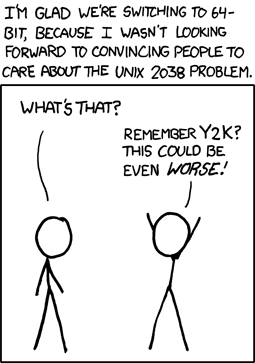
\includegraphics[width=.3\linewidth]{./gfx/xkcd-2038}
	\caption
	[Das \emph{Jahr 2038-Problem}]
	{Das \emph{Jahr 2038-Problem}. Quelle: \url{https://xkcd.com/607/}}
\end{center}
\end{figure}

\subsection{Zeitwerte finden und umrechnen}
Die aktuelle UNIX-Zeit wird von der Funktion \texttt{time} ermittelt. Dieser kann ein Pointer auf ein Objekt vom Typ \mintinline{c}{time_t} übergeben werden, an den die aktuelle Zeit (also die Zahl der Sekunden seit 1970-01-01, 00:00:00) geschrieben werden soll. Alternativ ist auch der Wert \texttt{NULL} als Parameter zulässig -- dann wird kein Wert in den Speicher geschrieben. In beiden Fällen enthält der Rückgabewert die Information der UNIX-Zeit.

\begin{codebox}[Beispiel: \texttt{time}]
\begin{minted}[linenos]{c}
#include <stdio.h>
#include <time.h>

int main () {
  time_t now = time(NULL);
  
  // time(&now);  // alternative Methode
  
  printf("%ld Sekunden seit 1970-01-01, 00:00:00.\n", now);
}
\end{minted}
\end{codebox}

Diese UNIX-Zeit kann nun in \enquote{menschliche Zeitrechnung} übersetzt werden, also in Jahre, Monate, \ldots aufgebrochen werden. Hierzu bedient man sich der Funktion \texttt{gmtime}, die einen Pointer auf ein Ojekt vom Typ \mintinline{c}{time_t} annimmt, und ein Objekt vom Typ \mintinline{c}{struct tm} zurück gibt. Dieser struct ist beschrieben unter \url{https://en.cppreference.com/w/c/chrono/tm} und enthält Felder für Jahr, Monat, Tag, \ldots. Mit \texttt{asctime} kann eine solches Objekt vom Typ 
\mintinline{c}{struct tm} in einen mit \texttt{printf} druckbaren Text umgewandelt werden (siehe \url{https://en.cppreference.com/w/c/chrono/asctime}).

\begin{codebox}[Beispiel: \texttt{time} in ein Datum übersetzen]
\begin{minted}[linenos]{c}
#include <stdio.h>
#include <time.h>

int main () {
  time_t now = time(NULL);
  printf("Now: %s", asctime(gmtime(&now)));
}
\end{minted}
\end{codebox}

\begin{cmdbox}[Ausgabebeispiel: \texttt{time} in ein Datum übersetzen]
Now: Fri Jun 21 19:50:01 2019
\end{cmdbox}

Um Objekte vom Typ \mintinline{c}{struct tm} zu erzeugen, sollte die Funktion \texttt{mktime} verwendet werden (\url{https://en.cppreference.com/w/c/chrono/mktime}). Die Funktion \texttt{strftime} erlaubt außerdem auch die Darstellung in anderen Zeit-Formaten als dem Amerikanischen (\url{https://en.cppreference.com/w/c/chrono/strftime}).

\subsection{Genaue Zeitmessung und Ticks}
Zeitangaben, die im Zusammenhang mit der UNIX-Zeit stehen sind nur auf eine Sekunde genau. Wo Genauigkeit auf unter eine Sekunde (und bis zu Nanosekunden hinab) gefragt ist, kann mit dem Datentyp \mintinline{c}{clock_t} gearbeitet werden. Auch hier handelt es sich um ein Alias für einen Ganzzahl-Datentyp. Mit Objekten dieses Typs werden aber nicht die Sekunden seit der UNIX-Epoche gezählt, sondern die \emph{Prozessortakte} seit einer bestimmten, nicht näher spezifizierten Referenzzeit. Üblichrweise ist diese Referenzzeit der Beginn der Ausführung des Programms.

Kennt man die Zahl der Prozessortakte, die in einer Sekunde umgesetzt werden, kann dies also leicht durch Division in eine Zeitdauer übersetzt werden. Genau diese Information -- Prozessortakte pro Sekunde -- ist in dem Macro \texttt{CLOCKS\_PER\_SEC} zugänglich:

\begin{codebox}[Beispiel: \texttt{clock}]
\begin{minted}[linenos]{c}
#include <stdio.h>
#include <time.h>
 
int main (void) {
  clock_t start = clock();
 
  // Zeitaufwändige Simulation
 
  clock_t end = clock();
  
  double cpu_time_used = ((double) (end - start)) / CLOCKS_PER_SEC; 
  printf("Die Simulation lief für %df Sekunden.\n", cpu_time_used);
}
\end{minted}
\end{codebox}

\subsection{Kurze Wartezeiten}
Manchmal möchte man den Ablauf seines Programms absichtlich verzögern. Dies könnte beispielsweise der Fall sein, wenn Sie ein Spiel programmieren, in dem Sie Ihren Spielern nicht Reaktionsvermögen einer CPU abverlangen wollen. 

Zu diesem Zweck existiert die Funktion \texttt{nanosleep}, die im POSIX-Standard von 1993 definiert wurde. Der Standard kann als Erweiterung zum C-Standard aufgefasst werden. Befehle, die hiervon abgedeckt werden gehören nicht mehr zum normalen Sprachumfang und werden nicht alleine durch Einbinden der richtigen Bibliotheken frei geschalten. Stattdessen muss eine Präprozessor-Konstante \texttt{\_POSIX\_C\_SOURCE} dem Compiler mitteilen, dass diese erweiterten Funktionen mit beachtet werden sollen\footnote{Im Header \texttt{<time.h>} finden Sie ein \mintinline{c}{#if}, das dafür sorgt, dass einige Definitionen nur umgesetzt werden, wenn die Präprozessor-Konstante einen geeigneten Wert hat.}.

Sobald \texttt{nanosleep} in Ihrem Code verfügbar gemacht wurde, können Sie es nach folgendem Beispiel benuzen:

\begin{codebox}[Beispiel: \texttt{clock}]
\begin{minted}[linenos]{c}
#define _POSIX_C_SOURCE 199309L   // this enables nanosleep
#include <time.h>

void   wait_ms(unsigned long miliseconds) {
  struct timespec sleeptime;
  
  if(miliseconds > 999) {   
    sleeptime.tv_sec  = (int) (miliseconds / 1000);
    sleeptime.tv_nsec = (miliseconds 
                      - ((long) sleeptime.tv_sec * 1000)) * 1000000;
  } else {   
    sleeptime.tv_sec = 0;
    sleeptime.tv_nsec = miliseconds * 1000000;
  }
  
  nanosleep(&sleeptime, NULL);
}
\end{minted}
\textrm{(Quelle:} \url{https://stackoverflow.com/questions/7684359}\textrm{)}
\end{codebox}

Eine genaue Beschreibung des Befehls finden Sie unter \url{http://man7.org/linux/man-pages/man2/nanosleep.2.html}

\begin{hintbox}[Es gäbe noch mehr zu sagen \ldots]
In diesem Abschnitt sollte Ihnen nur ein Überblick in die Logik hinter der time-library gegeben werden. Ich ermutige Sie also, selbstständig die unter \url{https://en.cppreference.com/w/c/chrono} aufgelisteten Funktionen selbstständig zu erkunden.
\end{hintbox}

\section{Zufallszahlen} \label{sec:RandomNums}
Computer sind \emph{deterministische} Maschinen. Das bedeutet, dass alle Ergebnisse, die mit einem Computer gewonnen werden können, bereits durch seinen Ausgangszustand vorgegeben sind. Kennt man den gesamten Speicherinhalt eines Rechners, so lässt sich daraus das Ergebnis jeder Berechnung und jedes Algorithmus ableiten. Dies schließt somit \emph{Zufall} bereits vollkommen aus.

Während \emph{echter} Zufall einem Computerprogramm nicht zugänglich ist, können wir aber zumindest Zahlenreihen erzeugen, die zufällig \emph{wirken}. Es ist einem Menschen \idR nicht möglich, die nächste Zahl einer solchen \emph{Pseudozufahlsreihe} vorherzusagen. In der Regel sind solche Zufallsreihen \emph{rekursiv} definiert, \ie eine Pseudozufallszahl wird aus ihrem Vorgänger berechnet. Damit gilt wieder, dass mit der ersten Zahl die komplette Zufallsreihe vorherbestimmt ist. Durch geschickte Wahl des Startwerts kann man aber echtem Zufall für die praktische Anwendung nahe genug kommen.

Im Header \texttt{<stdlib.h>} sind die Funktionen \texttt{rand} und \texttt{srand} deklariert, die zu diesem Zweck dienen. 
\begin{description}
\item[\texttt{rand}] gibt die nächste Zahl einer Zufallsreihe aus. Berechnet wird eine positive Ganzzahl zwischen 0 und \texttt{RAND\_MAX}. Letzteres wiederum ist ein Symbol, das ebenfalls in \texttt{<stdlib.h>} definiert ist, und dessen Wert von der Version des Compilers abhängt. I.\,d.\,R. handelt es sich um die größte Zahl, die mit dem Datentyp \mintinline{c}{int} dargestellt werden kann.
\item[\texttt{srand}] legt den Startwert fest. Als Argument wird eine vorzeichenlose Ganzzahl erwartet.
\end{description}

Es bietet sich an, als Startwert beispielsweise die aktuelle Systemzeit zu verwenden, wie sie von \texttt{time} zurück gegeben wird. Da dieser Wert im Allgemeinen bei jeder Programmausführung ein anderer ist, erhält man einen für praktische Zwecke gut geeigneten Pseudo-Zufallsgenerator.

In der praktischen Anwendung kann dies so aussehen:
\begin{codebox}[Beispiel: Pseudozufallszahlen]
\begin{minted}[linenos]{c}
#include <stdio.h>
#include <stdlib.h>
#include <time.h>

int main () {
  srand(time(NULL));      // "zufälligen" Startwert wählen
  
  printf("drei zufällige Ganzzahlen:\n");
  for (int i=0; i<3; i++) {
    printf("%d\n", rand());
  }
  
  printf("\ndrei zufällige Ganzzahlen zwischen 0 und 5:\n");
  for (int i=0; i<3; i++) {
    printf("%d\n", rand() % 6);
  }
  
  printf("\ndrei zufällige Fließkommazahlen zwischen 0 und 1:\n");
  for (int i=0; i<3; i++) {
    printf("%lf\n", (double) rand() / RAND_MAX);
  }
\end{minted}
\end{codebox}
%
\begin{codebox}[]
\begin{minted}[linenos, firstnumber=last]{c}
  
  double lo = 5;
  double hi = 15;
  printf("drei zufällige Fließkommazahlen zwischen %lf und %lf:\n", lo, hi);
  for (int i=0; i<3; i++) {
    printf("%lf\n", lo + ((double) rand() / RAND_MAX) * (hi-lo));
  }
}
\end{minted}
\end{codebox}

\begin{cmdbox}[Ausgabebeispiel: Zufallszahlen]
\begin{minted}{text}
drei zufällige Ganzzahlen:
1726242556
1893651755
1463512462

drei zufällige Ganzzahlen zwischen 0 und 5:
3
1
1

drei zufällige Fließkommazahlen zwischen 0 und 1:
0.662454
0.426405
0.427842

drei zufällige Fließkommazahlen zwischen 5.000000 und 15.000000:
5.544294
5.964819
9.742072
\end{minted}
\end{cmdbox}

\begin{hintbox}[Linear Congruential Generator -- der C-Standard-Pseudozufallsgenerator]
Der C-Standard schreibt nicht vor, wie der Algorithmus hinter \texttt{rand} genau auszusehen hat. Üblicherweise wird aber ein \emph{Linear Congruential Generator} implementiert. Diese funktionieren nach dem Prinzip:
\[ x_i = (a x_{i-1} + c) \mod m \]
Hierbei sind $x_i$ die berechneten Pseudozufallszahlen, \ie $x_{i-1}$ steht für den Vorgänger der gerade berechneten Zahl. Die Parameter $a$, $c$ und $m$ sind mehr oder minder beliebige Konstanten. Der Wert von $m$ legt den größten Wert fest, den diese Methode generieren wird. Eine geschickte Wahl von $a$ und $c$ sorgen für eine möglichst gleichmäßige Verteilung der Zufallswerte.

Der \texttt{gcc} verwendet:
\begin{align*}
	m &= 2^{31}\\
	a &= 1\,103\,515\,245\\
	c &= 12345
\end{align*}
(Siehe \url{https://en.wikipedia.org/wiki/Linear_congruential_generator})
\end{hintbox}

\begin{warnbox}[Statistische Qualität von Zufallszahlen]
Für allgemeine Anwendungen -- etwa die Programmierung von Spielen -- genügt der Standard-Zufallsgenerator des \texttt{gcc} vollkommen. Zu wissenschaftlichen Simulationen aber ist dieser \emph{nicht geeignet}. Die einzelnen Werte sind noch zu stark korrelliert, und die Periode (\ie die Zahl von Zufallswerten, bevor sich die Wertereihe wiederholt) ist zu gering.

Für Wissenschaftliche Arbeiten stehen viele Bibliotheken zur Verfügung, die ausgereiftere (aber auch langsamer arbeitende) Pseudozufalls-Generatoren anbieten. Ein Beispiel hierfür ist die \emph{Gnu Scientific Library} (GSL).

Siehe \url{https://www.gnu.org/software/gsl/}
\end{warnbox}

\section{\texttt{nan} -- not a number} \label{sec:NAN}
Fließkommazahlen -- also \mintinline{c}{float}s und \mintinline{c}{double}s -- haben eine interessante Eigenschaft: Sie können auch mathematische Objekte darstellen, die streng genommen \emph{keine Zahlen} sind. Bestimmte Bitmuster werden nicht als Zahl ausgewertet sondern stehen für das Ergebnis einer fehlerhaften Berechnung wie etwa die Wurzel aus einer negativen Zahl\footnote{C bietet zwar eine Bibliothek zur Arbeit mit komplexen Zahlen an. Für den \enquote{normalen} Betrieb gelten solche Rechnungen aber als nicht lösbar. Siehe dazu auch Abschnitt \ref{sec:complexNums}}. Wir nennen diese Bitmuster \emph{not a number} oder kurz \emph{NAN}.

Je nach Datentyp und Compiler werden unterschiedliche NANs unterschieden. Allen ist gemeinsam, dass jede Fließkomma-Rechnung, an denen eine NAN beteiligt ist, wieder eine NAN gleicher Art erzeugt. Soll eine solche NAN in eine Ganzzahl-Variable übertragen werden, so erzeugt dies, abhängig von Ziel-Datentyp und Compiler, entweder den Wert \texttt{0} oder $-2^{b}$ -- wobei $b$ die Breite des Datentyps in bits ist. Für \mintinline{c}{int}s (32bit) ergibt sich so der Wert \texttt{-2\,147\,483\,648}.

Bei der Ausgabe mit \texttt{printf} werden alle NANs durch die Zeichenkette \texttt{nan} dargestellt:
\begin{codebox}[Beispiel: NANs]
\begin{minted}[linenos]{c}
#include <stdio.h>
#include <math.h>

int main () {
  double nan = sqrt(-1.0);
  
  char         nan_char  = nan;
  short        nan_short = nan;
  int          nan_int   = nan;
  unsigned int nan_uint  = nan;
  long         nan_long  = nan;
  
  printf("nan als double: %lf\n" , nan      );
  printf("nan als char  : %hhd\n", nan_char );
  printf("nan als short : %hd\n" , nan_short);
  printf("nan als int   : %d\n"  , nan_int  );
  printf("nan als uint  : %d\n"  , nan_uint );
  printf("nan als long  : %ld\n" , nan_long );
  
  return 0;
}
\end{minted}
\end{codebox}

\begin{cmdbox}[Ausgabebeispiel: NANs]
\begin{minted}{text}
nan als double: nan
nan als char  : 0
nan als short : 0
nan als int   : -2147483648
nan als uint  : 0
nan als long  : -9223372036854775808
\end{minted}
\end{cmdbox}

Um zu überprüfen, ob ein Fließkommawert ein NAN ist (gleich welcher Art) kann das Macro \texttt{isnan} (definiert im Header \texttt{<math.h>}) benutzt werden:

\begin{codebox}[Beispiel: \texttt{isnan}]
\begin{minted}[linenos]{c}
#include <stdio.h>
#include <math.h>

int main () {
  printf("sqrt(+1.0)     ist %snan\n", (isnan(sqrt(+1.0)    ) ? "" : "kein "));
  printf("sqrt(-1.0)     ist %snan\n", (isnan(sqrt(-1.0)    ) ? "" : "kein "));
  printf("sqrt(-1.0) + 1 ist %snan\n", (isnan(sqrt(-1.0) + 1) ? "" : "kein "));
  
  return 0;
}
\end{minted}
\end{codebox}

\begin{cmdbox}[Ausgabebeispiel: \texttt{isnan}]
\begin{minted}{text}
sqrt(+1.0)     ist kein nan
sqrt(-1.0)     ist nan
sqrt(-1.0) + 1 ist nan
\end{minted}
\end{cmdbox}

Schließlich ist im Header \texttt{<float.h>} die Makro-Konstante \texttt{NAN} definiert, die zur schnellen bzw. klaren Erzeugung eines solchen Fehlerwerts geeignet ist.

\section{\texttt{atexit}}
Manche Aufgaben sollen erst ausgeführt werden, wenn das Programm beendet wird. Dies kann beispielsweise das Schließen von Logfiles sein oder die Freigabe von Speicherbereichen mit \texttt{free}.
Damit wir nicht jeden Pfad, auf den unser Programm enden kann, nachverfolgen müssen, können wir mit der Funktion \texttt{atexit} (deklariert im Heaer \texttt{<stdlib.h>}) eine oder mehrere eigene Funktionen registrieren, die bei Ende unseres Programms aufgerufen werden sollen.

Als Parameter wird ein Funktionszeiger auf eine \mintinline{c}{void}-Funktion ohne Parameter erwartet. (Da bei Programmende keine Stelle mehr einen Rückgabewert empfangen kann, ist der Rückgabetyp \mintinline{c}{void} naheliegend. Bedingt durch den automatischen Aufruf können auch keine Parameter übergeben werden. Werden in der Funktion dennoch zusätzliche Informationen gebraucht, muss dies über globale Variablen gelöst werden.)

\begin{codebox}[Beispiel: \texttt{atexit}]
\begin{minted}[linenos]{c}
#include <stdio.h>
#include <stdlib.h>

FILE * hDebug = NULL;

void handler_quit () {
  if (hDebug) {
    fclose(hDebug);
    printf("Debug Log geschlossen.\n");
  }
}

int main () {
  atexit(handler_quit);
  hDebug = fopen("debuglog.txt", "w");
  
  // restlicher Code...
}
\end{minted}
\end{codebox}


\section{Variadische Funktionen}
Wie wir wissen, können die Funktionen \texttt{printf} und \texttt{scanf} beliebig viele Parameter entgegen nehmen. Dies ist möglich, indem sie als \emph{variadische Funktionen} deklariert sind. Das bedeutet, dass ihre Signatur nur eine gewisse Anzahl an festen Parametern vorsieht und danach durch drei Punkte angedeutet wird, dass hier beliebige Werte folgen dürfen:

\begin{codebox}[Syntax: Prototyp einer variadischen Funktion]
\begin{minted}{c}
Rückgabetyp Funktionsname (Parameterliste_fest, ...);
\end{minted}
\end{codebox}

Um auf die so übergebenen \emph{variadischen Parameter} zuzugreifen, bietet der Header \texttt{<stdarg.h>} einge Macros an über die geeignete Pointer erhalten werden können.

Um die variadischen Parameter auszulesen benötigen wir zunächst ein Objekt vom Typ 
\mintinline{c}{va_list}, das als Handle auf die Parameter fungiert. Im folgenden soll diese Variable \texttt{args} genannt werden.

\texttt{args} wird über das Macro \mintinline{c}{va_start} initialisiert, dem wir dazu \texttt{args} als ersten Parameter übergeben mussen und zusätzlich den letzten Parameter, der \enquote{regulär} an unsere variadische Funktion übergeben wurde.

Einmal initialisiert liest das Macro \mintinline{c}{va_arg} nun aus \texttt{args} Werte beliebigen Typs aus. Als Parameter wird \texttt{arg} sowie der Datentyp des nächsten zu lesenden Wertes übergeben.
Ist die Arbeit mit der Liste beendet, muss mit \mintinline{c}{va_end} Speicher freigegeben werden.

Dieses abstrakte Vorgehen wird klarer, wenn wir ein Beispiel aus der CPP-Referenz betrachten:

\begin{codebox}[Beispiel: Variadische Funktion zum Aufsummieren beliebig vieler \texttt{int}s]
\begin{minted}[linenos]{c}
#include <stdio.h>
#include <stdarg.h>
 
int add_nums(int count, ...) {
  int result = 0;
  
  va_list args;                   // Liste variadischer Parameter
  va_start(args, count);          // Liste vorbereiten, Startpunkt nach count
  
  for (int i = 0; i < count; ++i) {
    result += va_arg(args, int);  // int-Werte aus der Liste lesen
  }
  
  va_end(args);
  return result;                  // Handle auf variadische Liste freigeben
}
 
int main() {
  printf("%d\n", add_nums(4, 25, 25, 50, 50));
}
\end{minted}
\end{codebox}

Besteht die variadische Liste aus Parametern unterschiedlichen Typs, so müssen die festen Parameter die Information enthalten, welche Datentypen an welcher Stelle der Liste stehen. Üblicherweise geschieht dies über einen \emph{Format String}. Die Interpretation eines solchen Strings nennt man auch \emph{parsen}.

\section{Komplexe Zahlen} \label{sec:complexNums}
Im Kontext von naturwissenschaftlichen Simulationen kommen häufig auch Rechnungen mit komplexen Zahlen vor. Der Header \texttt{<complex.h>} stellt einige Deklarationen und Makros bereit, die die Arbeit hiermit erleichtern.

Sobald der Header eingebunden ist, stehen die neuen Datentypen \mintinline{c}{complex float}, \mintinline{c}{complex double} und \mintinline{c}{complex long double} zur Verfügung. Wie ihre \enquote{Cousins} in den reellen Zahlen unterscheiden sich die drei Datentypen in der \emph{Rechengenauigkeit}, also in der Zahl der signifikanten Ziffern, die zur Verfügung stehen.

Mit Ausdrücken vom Typ \mintinline{c}{complex XXX} können die vier Grundrechenarten direkt mit den bekannten Operatoren (\texttt{+}, \texttt{-}, \texttt{*}, \texttt{/}) durchgeführt werden. Auch hier werden die gängigen Rechenregeln (Punkt vor Strich, Behandlung von Real- und Imaginärteil, \ldots) beachtet.

Der Header \texttt{<complex.h>} definiert auch das Symbol \texttt{I}, mit dem die imaginäre Einheit dargestellt wird. Mit den Funktionen \texttt{creal} und \texttt{cimag} kann der Real- bzw. Imaginärteil eines Ausdrucks vom Typ \mintinline{c}{complex XXX} ausgelesen werden.

Damit funktioniert dann der folgende Code:

\begin{codebox}[Beispiel: Grundrechenarten mit komplexen Zahlen]
\begin{minted}[linenos]{c}
#include <stdio.h>
#include <complex.h>

 
int main() {
  complex double z1 = 1.0 + 2.0 * I;
  complex double z2 = 5.0 - 2.7 * I;
  
  complex double z3 = z1 * z2 + z1;
  
  printf("Ergebnis: %lf%+lfi\n", creal(z3), cimag(z3));
}
\end{minted}
\end{codebox}

\begin{cmdbox}[Ausgabebeispiel: Grundrechenarten mit komplexen Zahlen]
Ergebnis: 11.400000+9.300000i
\end{cmdbox}

Für die wichtigsten aufwändigeren Operationen (Wurzel, Exponentialfunktion, Logarithmus, trigonometrische Funktionen, ...) existieren Analoga zu den bekannten Funktionen, die mit komplexen Zahlen funktionieren. Diese Funktionen haben denselben Namen wie die aus der \texttt{<math.h>} bekannten Routinen, beginnen aber mit dem Präfix \texttt{c}. Das bedeutet \eg, dass die Funktion \texttt{csin} den Sinus einer komplexen Zahl berechnet.

Um diese Funktionen benutzen zu können muss (wie auch schon bei den reellen mathematischen Funktionen) gegen die math-library gelinkt werden. Das heißt, der Compiler muss mit der Kommandozeilenoption \texttt{-lm} gestartet werden.

\begin{codebox}[Beispiel: Funktionen mit komplexen Zahlen]
\begin{minted}[linenos]{c}
#include <stdio.h>
#include <complex.h>
 
int main() {
  const int    lines     = 20;
  const double offset    = 40.0;
  const double height    = 10.0;
  const double frequency =  0.5;
  
  complex double result;
  
  for (int i=0; i<lines; i++) {
    result = cexp(i * frequency * I);
    
    for (int j=0; j<offset + creal(result) * height; j++) {
      printf(" ");
    }
    printf("*\n");
  }
}
\end{minted}
\end{codebox}

\begin{cmdbox}[Ausgabebeispiel: Funktionen mit komplexen Zahlen]
\begin{minted}{text}
                                                  *
                                                 *
                                              *
                                         *
                                    *
                                *
                               *
                               *
                                  *
                                      *
                                           *
                                                *
                                                  *
                                                  *
                                                *
                                            *
                                       *
                                  *
                               *
                               *
\end{minted}
\end{cmdbox}

Siehe \url{https://en.cppreference.com/w/c/numeric/complex} für eine Übersicht der komplexen Funktionen.

\section{Debugger}
Bis zu diesem Punkt haben Sie sicher schon festgestellt, wie häufig die ersten Zeilen Code, die wir schreiben fehlerhaft sind und nicht das Ergebnis erzielen, das wir uns erhoffen. Je größer und komplexer unsere Projekte werden, desto schwieriger wird es auch, einen Fehler ausfindig zu machen und zu korrigieren. Die Schwierigkeit besteht darin, die Entwicklung von den vielen Variablen nachzuverfolgen, mit denen wir arbeiten.

Um diese Aufgabe zu erleichtern steht das Tool \texttt{gdb} (GNU debugger) zur Verfügung. Das Programm wird von der Kommandozeile aufgerufen und bietet einen gewissen Einblick in unser laufendes Programm. Damit der Debugger diesen Einblick gewähren kann, müssen wir dem Compiler allerdings mitteilen, dass beim Übersetzen in Maschinensprache die Variablennamen und andere Informationen über unseren Quellcode erhalten bleiben sollen. Dies erreichen wir, indem wir den Compiler mit der Kommandozeilenoption \texttt{-g} aufrufen.

\begin{hintbox}[Performanz]
Programme, die mit der Debug-Option \texttt{-g} kompiliert wurden sind größer und laufen langsamer. Während der Entwicklung ist es sinnvoll, die Option zu nutzen, um eben den Support des \texttt{gdb} nutzen zu können. Vergessen Sie jedoch nicht, die finale Version ohne diese Option zu kompilieren, um das Maximum an Leistungsfähigkeit herauszuholen.
\end{hintbox}

Wenn Sie den \texttt{gdb} starten, finden Sie sich in einer neuen Kommandozeilen-Umgebung wieder. Das bedeutet, dass Sie, wie auch bei der Linux-Konsole, Kommandos eingeben und mit ENTER bestätigen können. Diese Kommandos sind jetzt jedoch andere, als dies in der normalen Konsole wäre.

Als ersten Schritt in der \texttt{gdb}-Umgebung können Sie mit dem folgenden Befehl festlegen, welches Programm Sie debuggen wollen:
\begin{cmdbox}[gdb: Programm festlegen]
file <executable>
\end{cmdbox}
Dabei steht \texttt{<executable>} für den Dateinamen Ihres \emph{ausführbaren} Programms. In den vorigen Beispielen wäre das also jeweils \texttt{./myProgram} gewesen.

Der Befehl \texttt{run} führt Ihr Programm aus. Sie können auch Kommandozeilenparameter an Ihr Programm übergeben, indem Sie diese hinter \texttt{run} setzen:
\begin{cmdbox}[gdb: Programm mit Kommandozeilenarametern starten]
run param1 param2 ...
\end{cmdbox}

Sie können im Vorfeld Punkte festlegen, an denen die Ausführung des Programms pausiert werden soll. Dies geschieht mit dem Befehl \texttt{break}. Hinter \texttt{break} können Sie entweder einen Funktionsnamen oder eine Zeilennummer angeben.

Ist ein solcher \emph{Breakpoint} erreicht, kann mit \texttt{print} der Wert von Variablen ausgegeben werden. Der folgende Befehl wird beispielsweise den Wert der Variablen \texttt{x} im aktuellen Zustand des Programms ausgeben:
\begin{cmdbox}[gdb: Wert von Variablen ausgeben]
print x
\end{cmdbox}

Schließlich lässt sich mit \texttt{continue} die Ausführung fortsetzen. Das Programm läuft weiter, bis ein neuer Breakpoint erreicht wird, bis das Programm regulär zu seinem Ende kommt oder bis es abstürzt.

Unter \url{https://web.eecs.umich.edu/~sugih/pointers/summary.html} finden Sie weitere Details zum GNU-Debugger.

\begin{hintbox}[Weitere Features]
Aus Gründen der Übersichtlichkeit können hier nur die wichtigsten Features des gdb vorgestellt werden. Dies soll aber nicht den Eindruck erwecken, dass der Funktionsumfang des Debuggers komplett durch einige zusätzliche \texttt{printf}-Zeilen im Code ersetzt werden könnte.
Lesen Sie beispielsweise unter \url{https://www.cs.umd.edu/~srhuang/teaching/cmsc212/gdb-tutorial-handout.pdf} über weitere Features des \texttt{gdb}.
\end{hintbox}
%
%\section{Die Bibliothek ncurses}
%
%\url{http://www.tldp.org/HOWTO/NCURSES-Programming-HOWTO/}
	\chapter{Rekursion} \label{chp:recursion}
\epigraph{To understand recursion, you must first understand recursion.}{Anonymous}

\begin{wrapfigure}{r}{.3\linewidth}
	\vspace{-10pt}
	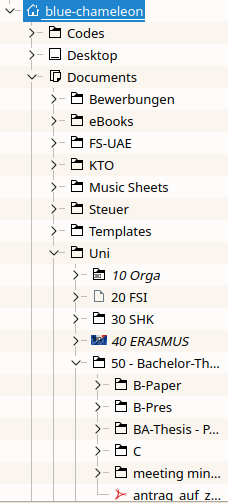
\includegraphics[width=\linewidth]{./gfx/foldertree}
	\caption
	[Auflistung einer Ordnerstruktur]
	{Die Auflistung einer Ordnerstruktur besteht aus Auflistungen von Sub-Ordnerstrukturen}
	\vspace{-90pt}
\end{wrapfigure}
Viele beim Programmieren auftauchende Probleme lassen sich in kleinere Unter-Probleme zerlegen, die dieselbe Form haben wie die ursprünglich zu lösende Aufgabe. Solche zerlegbaren Aufgaben lassen sich so weit aufdröseln, bis man bei einem \emph{elementaren Problem} angekommen ist, das mit einfachen Mitteln zu lösen ist.

Beispiel: Sie wollen die komplette Ordnerstruktur auf Ihrem Rechner auflisten. Dazu müssen Sie, ausgehend von einem Stammverzeichnis, ...
\begin{itemize}
\item alle Dateien des Stammverzeichnisses auflisten
\item alle Ordner im Stammverzeichnis auflisten
\item \emph{die Ordnerstruktur jedes Unterverzeichnisses auflisten}
\end{itemize}

In dieser Auflistung der Teilprobleme finden Sie also eine Unteraufgabe, die gleichlautend mit der ursprünglichen Aufgabe ist: Um eine Ordnerstruktur aufzulisten, müssen Sie eine \emph{Sub}-Ordnerstruktur auflisten. Die Teilaufgabe ist aber \enquote{leichter} als die Lösung des gesamten Problems, da nun nur eine Teilmenge des gesamten Ordnerstruktur aufgezählt werden muss. Schließlich wird man bei einer Teilaufgabe ankommen, die keine Sub-Ordnerstruktur mehr verlangt, da der Ausgangs-Ordner keine Unterordner mehr enthält. Die Auflistung eines solchen Ordners ohne Unterordner ist (verhältnismäßig) einfach.

Wir nennen Probleme, die sich auf gleichförmige Unterprobleme reduzieren lassen \emph{rekursiv}. Die entsprechende Lösungsstrategie nennt sich dementsprechend \emph{Rekursion}.

\section{Funktionen, die sich selbst aufrufen}
Behandeln wir zunächst ein einfaches Beispiel: Wir wollen alle Elemente eines \mintinline{c}{int}-Arrays aufsummieren. Natürlich können wir dies inzwischen schnell mit einer \mintinline{c}{for}-Schleife lösen. Für diesen Abschnitt wollen wir aber eine \emph{rekursive Strategie} wählen:

\begin{center}
\begin{minipage}{.8\linewidth}
\emph{Die Summe aller Elemente einer Liste ist gleich dem ersten Listenelement plus der Summe der verbleibenden Liste ohne ihr erstes Element.}
\end{minipage}
\end{center}

Diese Aufgabe ist direkt lösbar, wenn die verbleibende Liste nur ein Element hat. Ansonsten erkennen wir wieder die rekursive Struktur des Problems.

Zur Lösung setzen wir eine Funktion an, die als Parameter einen Pointer auf den Listenanfang sowie die Länge der Liste erwartet. Diese Funktion wird \emph{sich selbst aufrufen}, also \emph{in die Rekursion gehen}.

\begin{codebox}[Beispiel: Rekursives Aufsummieren]
\begin{minted}[linenos]{c}
#include <stdio.h>

int listsum_recursive(int * list, unsigned int N) {
  if        (N == 1) {
    return list[0];
    
  } else if (N == 2) {
    return list[0] + list[1];
    
  } else {
    return list[0] + listsum_recursive(list + 1, N - 1);
  }
}

int main () {
  int list[] = {1, 2, 3, 4, 5, 6, 7, 8, 9};
  
  printf("Summe: %d\n", listsum_recursive(list, sizeof(list) / sizeof(*list)));
  return 0;
}
\end{minted}
\end{codebox}

\begin{cmdbox}[Ausgabebeispiel: Rekursives Aufsummieren]
Summe: 45
\end{cmdbox}

Wie nun funktioniert dieses Verfahren?

Die Zeilen 1 bis 8 sind unkompliziert. Der Fall einer Liste mit nur einem bzw. zwei Elementen wird mit elementaren Mitteln bearbeitet. Für den interessanten Fall, dass die Unterliste mehr als ein Element hat (\mintinline{c}{else} in Zeile 10) beschreiben wir die Rekursionsstrategie: Wir addieren das erste Listenelement \texttt{list[0]} zur Summe der Unterliste ohne dieses erste Element. Der Ausdruck \texttt{list + 1} beschreibt einen \mintinline{c}{int}-Pointer, der um ein \mintinline{c}{int}-Element gegenüber der ursprünglichen Liste verschoben ist. \texttt{list + 1} zeigt also auf eine \enquote{neue} Liste, die mit dem \emph{zweiten} Element von \texttt{list} beginnt.

In der Umsetzung werden in Zeile 11 die beiden Summanden getrennt voneinander ausgewertet. Das heißt, der Rechner liest den Wert \texttt{list[0]} aus dem Speicher. Die Auswertung des zweiten Summanden sieht (\emph{in Pseudo-Syntax, \ie in nicht gültigem C-Code!}) so aus:

\begin{codebox}[Auswertung: Rekursionsstufe 0 in Pseudosyntax]
\begin{minted}{c}
    return 1 + listsum_recursive({2, 3, 4, 5, 6, 7, 8, 9}, 8);
\end{minted}
\end{codebox}

Als \texttt{Rekursionstiefe} oder \emph{Rekursionsebene} bezeichen wir die Anzahl der \enquote{verschachtelten} Aufrufe. Da wir aus der Funktion \texttt{listsum\_recursive} wieder dieselbe Funktion \texttt{listsum\_recursive} aufrufen, haben wir also gerade Rekursionsebene 1 erreicht.

Natürlich muss jetzt noch der Funktionsaufruf von \texttt{listsum\_recursive} aufgelöst werden. Dies geschieht nach demselben Prinzip wie schon der erste Aufruf, der von der \texttt{main} aus gestartet wurde. Wir gehen also wieder eine Rekursionsebene tiefer, wenn wir wieder auf Zeile 11 treffen. Die Zeile wird dann ausgewertet zu:

\begin{codebox}[Auswertung: Rekursionsstufe 1 in Pseudosyntax]
\begin{minted}{c}
    return 2 + listsum_recursive({3, 4, 5, 6, 7, 8, 9}, 7);
\end{minted}
\end{codebox}

Auch wenn wir immer dieselbe Funktion aufgerufen, wird jeweils ein neuer Scope betreten. Die Bezeichner \texttt{N} und \texttt{list} stehen also auf jeder Rekursions-Ebene für andere Speicherstellen. Sie können sich dies wie verschachtelte Boxen:

\begin{codebox}[Rekursionsstufe 0: Symbol und Werte]
N = 9, list = \{1, 2, 3, 4, 5, 6, 7, 8 ,9\}
\begin{codebox}[Rekursionsstufe 1: Symbole und Werte]
N = 8, list = \{2, 3, 4, 5, 6, 7, 8 ,9\}
\begin{codebox}[Rekursionsstufe 2: Symbole und Werte]
N = 7, list = \{3, 4, 5, 6, 7, 8 ,9\}
\begin{codebox}[Rekursionsstufe 3-6]
...
\begin{codebox}[Rekursionsstufe 7: Symbole und Werte]
N = 2, list = \{8, 9\}
\end{codebox}
\end{codebox}
\end{codebox}
\end{codebox}
\end{codebox}

Obwohl wir formell in derselben Funktion bleiben, hat das Symbol \texttt{N} in Ebene 7 und Ebene 6 nichts miteinander zu tun. Dasselbe gilt für das Symbol \texttt{list}.

In Ebene 7 treffen wir endlich auf einen Fall, den unser Algorithmus ohne weiteren Rekursionsschritt auskommt. Es wird die Summe \texttt{8 + 9} berechnet und zurück gegeben. Dieser Rückgabewert wird nun in Zeile 11 der jeweils übergeordneten Rekursionsebene eingesetzt, um auch dort einen Rückgabewert zu berechnen. Der Stapel wird sozusagen \emph{von innen heraus} aufgelöst:

\begin{codebox}[Rekursionsstufe 0: Rückgabewerte]
\begin{codebox}[Rekursionsstufe 1: Rückgabewerte]
\begin{codebox}[Rekursionsstufe 2: Rückgabewerte]
\begin{codebox}[Rekursionsstufe 3-6]
\begin{codebox}[Rekursionsstufe 7: Rückgabewerte]
return 8 + 9;
\end{codebox}
...
\end{codebox}
return 3 + 39;
\end{codebox}
return 2 + 42;
\end{codebox}
return 1 + 44;
\end{codebox}

\begin{warnbox}[Pseudocode und tatsächliche Werte]
Im obigen Beispiel wurde der Anschaulichkeit halber \texttt{list} mit einer Menge von Werten ersetzt (Darstellung in \{geschweiften Klammern\}). Dies ist keine gültige C-Syntax!

In der Realität wird jeweils ein \emph{Pointer} an die untergeordnete Rekursionsebene weitergeleitet. Alle diese Pointer zeigen auf \emph{überlappende} Speicherbereiche, sind aber jeweils um die Speicherbreite einer Zahl gegeneinander verschoben. Da man nun verschiedene Speicherpunkte als Listen-Anfang interpretiert, und zugleich die Listenlänge \texttt{N} in jeder Rekursionsebene um 1 reduziert, ergeben sich effektiv die oben gezeigten Listen.

Während die oben gewählte Darstellung die Vorgänge klarer macht, sollten Sie sich bewusst sein, was tatsächlich im Speicher abgelegt wird.
\end{warnbox}

\section{Kommunikation über Rekursionsebenen hinweg}
Wie üblich bei Funktionsaufrufen können Sie Werte zwischen den Rekursionsebenen austauschen, indem Sie diese als Parameter übergeben. Dies ist aber nicht immer wünschenswert. Stellen Sie sich etwa vor, Sie wollen eine Sicherheitssperre einbauen und die Rekursionstiefe auf 10 begrenzen. Dies ist möglich über folgenden Ansatz:

\begin{codebox}[Beispiel: Rekunsionstiefe mit Parameter]
\begin{minted}[linenos]{c}
int recursiveFunc(unsigned int depth) {
  if (depth > 10) {return 0;}
  
  depth++;
  recursiveFunc(depth)
  
  // nützlicher Code...
  
  return 1;
}
\end{minted}
\end{codebox}

Allerdings müssen Sie hier beim Aufruf der Funktion \texttt{recursiveFunc} (\eg aus der \texttt{main} heraus) den dort bedeutungslosen Parameter \texttt{depth} angeben. Um dem zu entgehen, können Sie auch das Schlüsselwort \mintinline{c}{static} benutzen.

Wie Sie noch aus Abschnitt \ref{sec:staticVar} wissen, sorgt \mintinline{c}{static} dafür, dass die Speicherzelle für ein so deklariertes Symbol nicht freigegeben wird, wenn die Funktion verlassen wird, dass also der Wert des Symbols zwischen Funktionsaufrufen erhalten bleibt. In diesem Fall bedeutet das also, dass der Wert eines \mintinline{c}{static} Symbols auch über die Rekursionsebenen hinweg erhalten bleibt. Somit können wir das obige Beispiel auch \emph{ohne} Parameter umsetzen:

\begin{codebox}[Beispiel: Rekunsionstiefe ohne Parameter]
\begin{minted}[linenos]{c}
int recursiveFunc() {
  static int depth = 0;
  
  if (depth > 10) {return 0;}
  
  depth++;
  recursiveFunc()
  depth--;
  
  // nützlicher Code...
  
  return 1;
}
\end{minted}
\end{codebox}

Zeile 2 -- die Deklaration und Wertzuweisung von \texttt{depth} wird nur ein einziges Mal\footnote{und tatsächlich bereits zur Kompilierzeit} ausgeführt. Ab dann greift \texttt{depth} von jeder Rekursionsebene auf \emph{dieselbe} Speicherstelle zu. Die Verwendung ist also ähnlich einer globalen Variablen, die aber nur innerhalb von \texttt{recursiveFunc} \enquote{sichtbar} ist.

\section{Laufzeitverhalten von rekursiven Methoden}
Wie Sie wissen, bedeuten Funktionsaufrufe einigen Verwaltungsaufwand, der in Summe spürbar Zeit kosten kann. Hinzu kommt, dass die maximale Rekursionstiefe begrenzt ist, da für jeden Rekursionsschritt gespeichert werden muss, wo die Programmausführung nach Ende eines Rekursionsschritts fortgesetzt werden soll. Diese \emph{Rücksprung-Adresse} wird auf dem Stack abgelegt, der nur begrenzt Speicherplatz anbietet. Zu viele Rekursionsebenen\footnote{mehrere hundert} führen zu einem sogenannten \emph{Stack overflow}.

Es lässt sich beweisen, dass jeder \emph{rekursive Algorithmus} sich auch in verschachtelten Schleifen schreiben lässt. Wo dies \emph{einfach} möglich ist, ist eine solche Lösung ohne Rekursion auch zu bevorzugen. Das obige Beispiel der Summe über ein Array sollte also aus Effizienzgründen besser so implementiert werden:

\begin{codebox}[Beispiel: Iteratives Aufsummieren]
\begin{minted}[linenos]{c}
#include <stdio.h>

int listsum_iterative(int * list, unsigned int N) {
  int reVal = 0;
  
  for (unsigned int i=0; i<N; i++) {
    reVal += list[i];
  }
  
  return reVal;
}

int main () {
  int list[] = {1, 2, 3, 4, 5, 6, 7, 8, 9};
  
  printf("Summe: %d\n", listsum_iterative(list, sizeof(list) / sizeof(*list)));
  return 0;
}
\end{minted}
\end{codebox}

Häufig macht eine rekursive Formulierung den Algorithmus aber für \emph{Menschen} leichter verständlich, und damit auch besser wartbar, erweiterbar oder anpassbar. Dies gilt insbesondere dann, wenn die Problembeschreibung bereits rekursive Elemente enthält, bzw. wenn sich die Aufgabe in \emph{Hierarchie-Ebenen} einteilen lässt. Im folgenden Abschnitt werde ich Ihnen eine rekursive Lösung zum Beispiel am Anfang des Kapitels zeigen. Ich lade Sie dazu ein, diese Lösung in eine nicht-rekursive Form umzuschreiben.

\section{Beispiel: Rekursives Auflisten der Ordnerstruktur}
Der folgende Code ist länger und verwendet einige Befehle, die hier noch nicht besprochen wurden. Sie werden aber feststellen, dass Sie inzwischen die Funktionsweise des Codes erfassen können, auch wenn Sie nicht jedes Detail verstehen. Die Namen der einzelnen Symbole sind dabei so gewählt, dass Ihnen das Verständnis erleichtert wird, wie es auch allgemein gute Praxis ist. Kommentare ergänzen dabei schwerer erfassbare Elemente in knapper Form.

Beginnen Sie beim Nachvollziehen mit der Funktion \texttt{showtree} ab Zeile 186. Diese enthält die Rekursion und ist für dieses Kapitel die interessanteste Funktion. Die Funktion \texttt{print\_indented} ab Zeile 178 sollte Ihnen keine Probleme bereiten.

Fahren Sie dann fort mit der Definition von \texttt{stringlist} und den zugeordneten Funktionen \texttt{make\_stringlist}, \texttt{free\_stringlist}, \texttt{append\_to\_stringlist}, 
\texttt{get\_stringlist\_item} und \texttt{get\_stringlist\_length} in der abgedruckten Reihenfolge. Diese führen einen eigenen Datentyp mit zugehörigen Funktionen ein und illustrieren eine gängige Herangehensweise in der Programmiertechnik: in ihren Eigenschaften eine Einheit bildene Informationen werden zu einem \emph{Objekt} zusammengefasst. Die daran auftretenden Aufgaben werden von allgemein gefassten \emph{Methoden} (Funktionen) erledigt\footnote{Man spricht auch von \emph{Reifikation}, oder \enquote{Verdinglichung}. In Kursen zur \emph{Objektorientierten} Programmierung wie in C++ ist dies ein zentrales Konzept}.

Die Funktion \texttt{get\_directory\_entries} ist auf Anhieb vermutlich schwer zu erfassen, da hier die meisten bisher unbekannten Befehle auftauchen. Ich werde nach dem Code einige Erläuterungen dazu geben. Versuchen Sie aber zuerst, die Zusammenhänge selbst zu erahnen.

\subsection{Code}
\begin{codebox}[Beispielprogramm: \texttt{tree.c}]
\begin{minted}[linenos]{c}
#define _GNU_SOURCE       // use all features from unistd.h

#include <stdio.h>
#include <stdlib.h>
#include <string.h>
#include <unistd.h>       // some file system functions...
#include <dirent.h>       // ... and some more ...
#include <sys/stat.h>     // ... and even more.

// ========================================================================= //
// handle a list of strings

typedef struct {
  unsigned int N;       // number of strings in the list
  char **      items;   // the list itself
} * stringlist;

// ------------------------------------------------------------------------- //

stringlist make_stringlist() {
  /* Create a well-defined initial state so that the other methods don't have
   * to do excessive error-checking
   */
  
  stringlist reVal = malloc(sizeof(stringlist));
  
  if (reVal) {
    reVal->N     = 0;
    reVal->items = NULL;
  } else {
    printf("Error in make_stringlist: Could not allocate memory.\n");
    return NULL;
  }
  
  return reVal;
}

// ......................................................................... //
\end{minted}
\end{codebox}

\begin{codebox}[]
\begin{minted}[linenos, firstnumber=last]{c}
void free_stringlist(const stringlist list) {
  /* frees all memory occupied by the components of a stringlist.
   */
  
  // first, free the items themselves
  for (unsigned int i=0; i<list->N; i++) {
    if (list->items[i]) {free(list->items[i]);}
  }
  
  // then free the list of items
  free(list->items);
  
  // and finally, free the struct
  free(list);
}

// ......................................................................... //

int append_to_stringlist(const stringlist list, const char * item) {
  /* adds an item to the end of a stringlist.
   * returns number of items in the list on success or -1 on failure.
   */
  
  // check whether a NULL pointer was passed
  if (!list) {
    printf("Error in append_to_stringlist: Invalid list.\n");
    return -1;
  }
  
  // make a copy of the item to be added to the list
  char * newItem = malloc(strlen(item) + 1);
  if (!newItem) {
    printf("Error in append_to_stringlist: Not enough memory for new item.\n");
    return -1;
  }
  strcpy(newItem, item);
  
  // make the list one item longer
  char ** longerList = realloc(list->items, (list->N+1) * sizeof(*longerList));
  if (!longerList) {
    printf("Error in append_to_stringlist: Could not expand list.\n");
    free(newItem);
    return -1;
  }
  
  list->items = longerList;
  list->items[list->N] = newItem;
  
  return ++list->N;
}

// ......................................................................... //
\end{minted}
\end{codebox}

\begin{codebox}[]
\begin{minted}[linenos, firstnumber=last]{c}
char * get_stringlist_item(const stringlist list, const unsigned int i) {
  /* access to stringlist items with error checks
   */
  
  // check whether a NULL pointer was passed
  if (!list) {
    printf("Error in get_stringlist_item: Invalid list.\n");
    return NULL;
  }
  
  // check if index out of boundaries
  if (i < list->N) {
    return list->items[i];
    
  } else {
    printf("Error in get_stringlist_item: Invalid index.\n");
    return NULL;
  }
}

// ......................................................................... //

unsigned int get_stringlist_length(const stringlist list) {
  if (!list) {
    printf("Error in get_stringlist_length: Invalid list.\n");
    return 0;
  }
  
  return list->N;
}

// ========================================================================= //
// create lists of files and directories in the current working directory

typedef enum {listtype_files, listtype_directories} listtypes;

stringlist get_directory_entries (const listtypes type) {
  stringlist reVal = make_stringlist();
  
  DIR * filesystem_handle = opendir(".");
      // "." represents current work directory
      // opendir returns NULL if it couldn't open the directory 
  
  struct dirent * directory_entry;
      // will hold name of one item in the directory
  struct stat     statbuffer;
      // will hold kind of one item in the directory (file or folder)
  
  if (filesystem_handle == NULL) {
    printf("Error in get_subdirectories: Could not open current directory\n");
    free_stringlist(reVal);
    return NULL;
  }
\end{minted}
\end{codebox}

\begin{codebox}[]
\begin{minted}[linenos, firstnumber=last]{c}
  // read new entries from the directory as long as there are any.
  while (  (directory_entry = readdir(filesystem_handle)) != NULL  ) {
    // skip special file system elements
    if ((strcmp(directory_entry->d_name, "." ) == 0) ||
        (strcmp(directory_entry->d_name, "..") == 0)
    ) {continue;}
    
    // analyze type of directory enty
    if(  stat(directory_entry->d_name, &statbuffer) == -1  ) {
      printf("Error in get_subdirectories: "
             "Could not determine kind of entry %s\n", 
             directory_entry->d_name);
      free_stringlist(reVal);
      return NULL;
    }
    
    int entry_is_directory = S_ISDIR(statbuffer.st_mode);
    int condition_to_add =
       ( entry_is_directory && (type == listtype_directories)) ||
       (!entry_is_directory && (type == listtype_files      ));
    
    if (condition_to_add) {
      append_to_stringlist(reVal, directory_entry->d_name);
    }
    
  }
  
  closedir(filesystem_handle);
  return reVal;
}

// ========================================================================= //
// recursive traversal of file system

void print_indented(const char * text, const unsigned int n) {
  for (unsigned int i=0; i<n; i++) {printf("  ");}
  
  printf("%s\n", text);
}

// ------------------------------------------------------------------------- //

void showtree(char * startDir) {
  static unsigned int indent_level = 0;
  int                 flag_free_startDir = 0;
  
  if (!startDir) {
    // use current work directory if nothing else was specified.
    startDir = get_current_dir_name();
        // this function uses malloc, thus a free() is needed later
    flag_free_startDir = 1;
        // store information: free is needed.
  }
\end{minted}
\end{codebox}

\begin{codebox}[]
\begin{minted}[linenos, firstnumber=last]{c}
  if (  chdir(startDir)  ) {
    // switch to directory startDir. Return 0 on success, -1 otherwise
    
    printf("\x1b[91m");   // switch to colour red for error output
    print_indented("(invalid directory)", indent_level);
    printf("\033[m");     // restore normal colours
    if (flag_free_startDir) {free(startDir);}
    return;
  }
  
  printf("\x1b[96m");   // show directories in bright cyan
  print_indented(startDir, indent_level);
  printf("\033[m");     // restore normal colours
  
  // get list of directories and go into recursion
  stringlist subdirs = get_directory_entries(listtype_directories);
  if (subdirs) {
    for (unsigned int i=0; i<get_stringlist_length(subdirs); i++) {
      indent_level++;
      showtree(get_stringlist_item(subdirs, i));
      chdir("..");
      indent_level--;
    }
    free_stringlist(subdirs);
  }
  
  // get list of files
  stringlist files = get_directory_entries(listtype_files);
  if (files) {
    for (unsigned int i=0; i<get_stringlist_length(files); i++) {
      print_indented(get_stringlist_item(files, i), indent_level + 1);
    }
    free_stringlist(files);
  }
  
  if (flag_free_startDir) {free(startDir);}
}

// ========================================================================= //

int main (int argc, char ** argv) {
  if (argc) {showtree(argv[1]);}
  else      {showtree(NULL   );}
}
\end{minted}
\end{codebox}

\subsection{Anmerkungen zu \texttt{showtree}}
Als Parameter wird dieser Funktion ein \mintinline{c}{char *} übergeben, also ein String. Dieser benennt das Ausgangsverzeichnis, von dem ab die Auflistung der Ordnerstruktur beginnen soll. Neben einem \enquote{sinnvollen} Pointer auf eine echte Zeichenkette kann aber auch der Wert \texttt{NULL} übergeben werden. In diesem speziellen Fall wird der Rechner angewiesen, vom aktuellen Arbeitsverzeichnis auszugehen. Der Name desselben wird mit der Funktion \texttt{get\_current\_dir\_name} ermittelt. Die Funktion ist im Header \texttt{<unistd.h>} deklariert, sobald das Macro \texttt{\_GNU\_SOURCE} definiert wird.

Wie Sie unter \url{http://man7.org/linux/man-pages/man3/getcwd.3.html} nachlesen können, reserviert \texttt{get\_current\_dir\_name} für den Namen des aktuellen Arbeitsverzeichnisses Speicher, der später wieder mit \texttt{free} freigegeben werden muss. Wir \emph{setzen ein Flag}, \ie speichern die Information, dass wir dieses \texttt{free} später noch ausführen müssen in einer Variablen \texttt{flag\_free\_startDir}.

Die \mintinline{c}{static unsigned int indent_level} speichert die gegenwärtige Rekursionstiefe. Wir benutzen diese Information auch, um damit Einrückungen zu machen, und die hierarchische Struktur des Ordnersystems grafisch wiedergeben.

In Zeile 197 wird \texttt{chdir} aufgerufen. Auch diese Funktion ist im Header \texttt{<unistd.h>} deklariert, und setzt ein neues Arbeitsverzeichnis. Da \texttt{startDir} auch auf \enquote{unsinnige} Strings zeigen kann, ist es möglich, dass dieser Verzeichniswechsel fehlschlägt. In diesem Fall ist der Rückgabewert von \texttt{chdir} gleich \texttt{-1}\footnote{Daneben sind auch andere Wege möglich, wegen derer der Verzeichniswechsel fehlschlagen kann. Beispielsweise kann der Zugriff auf einzelne Verzeichnisse nur dem Administrator gestattet sein, oder ein Netzlaufwerk ist wegen schlechter Verbindung zeitweise nicht erreichbar.}.
Lesen Sie hierzu mehr unter \url{http://man7.org/linux/man-pages/man2/chdir.2.html}.

Beachten Sie Zeile 201: Obwohl wir die Funktion \texttt{print\_indented} bislang noch nicht besprochen haben, dürften Sie intuitiv erfassen, was hier geschieht: Der Text \texttt{(invalid directory)} wird auf dem Bildschirm ausgegeben, und zwar mit einer Einrückung, die der aktuellen Tiefe im Ordnerbaum entspricht. Dass der Effekt ohne genauere Betrachtungen erfasst werden kann ist eine Konsequenz aus der sinnvollen Benennung von Funktionen und Variablen.

Ähnlich verhält es sich mit Zeile 212:
\begin{center}
\mintinline{c}{stringlist subdirs = get_directory_entries(listtype_directories);}
\end{center}
Eine neue Variable vom Typ \texttt{stringlist} mit Namen \texttt{subdirs} wird angelegt und speichert nun den Wert, der von \texttt{get\_directory\_entries(listtype\_directories)} berechnet wurde. Obwohl wir bislang weder wissen, wie dieser Typ \texttt{stringlist} aufgebaut ist, noch wie exakt 
\texttt{get\_directory\_entries} funktioniert, können wir diese Zeile \emph{semantisch} erfassen: gespeichert werden alle Einträge des aktuellen Arbeitsverzeichnisses, die dem 
\texttt{listtype\_directories} entsprechen, also alle Unterordner des aktuellen Arbeitsverzeichnisses.

Wenn diese \texttt{stringlist} nicht leer war (Zeile 213), so wird jedes Element der Liste abgearbeitet. Da dies bei Unterordnern bedeutet, dass wir eine Ebene tiefer in die Rekursion gehen, erhöhen wir zuerst den Zähler \texttt{indent\_level}, bevor wir rekursiv wieder \texttt{showtree} aufrufen. Statt im aktuellen Arbeitsverzeichnis zu starten, geben wir nun aber als Parameter 
\texttt{get\_stringlist\_item(subdirs, i)} an: der \texttt{i}-te Wert aus der Liste \texttt{subdirs}, also der Name des Unterordners, den wir gerade analysieren wollen. In diesem Rekursionsschritt wird unsere Funktion ein \texttt{chdir} ausführen, und so in das Unterverzeichnis wechseln. Wenn die Struktur des Unterverzeichnisses ausgegeben wurde, müssen wir natürlich wieder ins Ausgangsverzeichnis zurückkehren. Dazu dient in Zeile 217 der Befehl \texttt{chdir("..");}. Mit dem Wechsel ins Ausgangsverzeichnis sind wir auch wieder eine Hierarchieebene aufgestiegen; daher reduzieren wir den Zähler \texttt{indent\_level}. Die Liste \texttt{subdirs} hat Speicherplatz beansprucht, der von hier an nicht mehr gebraucht wird. Da anscheinend die Struktur des Typs \texttt{stringlist} etwas komplexer ist, existiert zu diesem Zweck eine eigene Funktion \texttt{free\_stringlist}, die für uns diesen \enquote{Aufräumvorgang} erledigt.

Für die Ausgabe der Dateien passiert nochmals dasselbe, nur dass hier kein Rekursionsschritt mehr erfolgt. Stattdessen werden alle Dateien auf dem Bildschirm mit Hierarchieebene 
\texttt{indent\_level + 1} ausgegeben, um zu symbolisieren, dass sie eben \emph{unter} dem gerade analysierten Verzeichnis zu finden sind.

\subsection{Anmerkungen zur \texttt{stringlist}}
Wir haben bereits gesehen, dass es leicht nachzuvollziehen ist \emph{was} die \texttt{stringlist} für uns leistet. Nun wollen wir verstehen, \emph{wie} die umgesetzt wird.

In den Zeilen 13 bis 16 wird der Typ \texttt{stringlist} über ein \mintinline{c}{typedef} definiert. Es handelt sich um einen \emph{Pointer auf} eine \mintinline{c}{struct} mit zwei Feldern: \texttt{N}, das die Zahl der Listenelemente speichert und \texttt{items}, welches die eigentliche Liste enthält. Da es sich um eine Liste von \emph{Strings} handelt, muss der Datentyp von \texttt{items} \mintinline{c}{char **} sein.

Es ist in C üblich, bei komplexen Objekten den zugehörigen Datentyp gleich als Pointer anzulegen. Dies erlaubt, dass Funktionen Änderungen am Objekt durchführen (\eg Listenelemente einfügen), ohne dass hierfür explizit der Adressoperator \texttt{\&} benutzt werden müsste, und erlaubt eine komfortablere Anwendung.

Um ein Objekt vom Typ \texttt{stringlist} zu erzeugen, das \enquote{sinnvolle} Werte hat, finden wir in Zeile 20 die Funktion \texttt{make\_stringlist}. Sie reserviert zuerst den Speicherplatz für die Struktur selbst. War dies erfolgreich, setzen wir die Startwerte auf \texttt{N=0} und \texttt{items} auf einen den Wert \texttt{NULL}. Andernfalls wird auf dem Bildschirm eine Fehlermeldung ausgegeben und der Rückgabewert der Funktion \texttt{NULL} gesetzt. Damit kann auch nicht versehentlich mit zufällig im Speicher befindlichen Werten weiter gearbeitet werden.

Verwandt mit \texttt{make\_stringlist} ist \texttt{free\_stringlist}: Diese Funktion gibt allen Speicher frei, der von unserer Liste in Anspruch genommen wurde. Dies umfasst den Speicher für die einzelnen Strings, für die Liste der Strings, und für die Datenstruktur \texttt{stringlist} selbst.

Das Paar \texttt{make\_stringlist} und \texttt{free\_stringlist} kann man als \emph{Constructor und Destructor} auffassen. Beides sind Begriffe aus C++ bzw. der objektorientierten Programmierung; dem Konzept nach erledigen diese beiden Funktionen aber dieselbe Aufgabe, nämlich das Erstellen und Bereinigen einer Datenstruktur vor bzw. nach Gebrauch.

Spannend ist nun die Funktion \texttt{append\_to\_stringlist}: Nach einer Sicherheitsprüfung in Zeile 63 wird zunächst eine Kopie des Elements angelegt, das wir an unsere Liste anhängen wollen (ab Zeile 69). Dies müssen wir tun, da unser Destructor explizit auch den Speicherplatz für die Strings in der Liste wieder freigibt. Wenn wir nun Pointer auf Strings übergeben, die nicht freigegeben werden dürfen (\eg String Literals), würde dies zu einem Programmabsturz führen. Stattdessen gestalten wir unsere Routinen so, dass sie eine \emph{geschlossene Einheit} bilden. Parameter, die \emph{von außen} übergeben werden, also aus anderen Programmteilen stammen werden nur gelesen, nicht aber verändert. Wir sagen, \emph{die \texttt{stringlist} verwaltet sich selbst}.

In Zeile 77 wird nun versucht, die Liste zu erweitern. Wir benutzen dazu \texttt{realloc} und speichern das Ergebnis dieses Versuchs zunächst in \texttt{longerList} zwischen. Dies hat folgenden Grund:

Stellen Sie sich vor, die Erweiterung schlägt fehl. Es kann zwar kein Speicher für \texttt{N+1} \mintinline{c}{char *} gefunden werden; die alte Liste bleibt aber dennoch bestehen. Hätten wir also \texttt{items} direkt überschrieben, so hätte dieses Element jetzt den Wert \texttt{NULL}, und der Zugriff auf die alte Liste wäre verloren. Insbesondere könnte auch der hierfür reservierte Speicher nicht mehr freigegeben werden. 

Wenn die Liste nicht erweitert werden kann, so ist auch unsere Kopie \texttt{newItem} überflüssig geworden und muss mit \texttt{free} freigegeben werden.

Haben dagegen alle Speicher-Allozierungen funktioniert, so können in unserer \texttt{stringlist list} die Änderungen eingetragen werden: \texttt{items} erhält nun die neue Adresse, die wir in \texttt{longerList} zwischengespeichert hatten. An das Ende der Liste wird \texttt{newItem} gestellt. Da wir den Zähler \texttt{N} noch nicht erhöht haben, ist \texttt{N} auch Index des letzten Elements.

In Zeile 87 erhöhen wir endlich auch diesen Zähler und geben die neue Anzahl der Elemente in der Liste zurück.

\texttt{get\_stringlist\_item} und \texttt{get\_stringlist\_length} bieten lediglich ein komfortableres Interface auf unsere Datenstruktur: Einige Sicherheitsprüfungen werden durchgeführt, außerdem sind die Namen leichter interpretierbar als \texttt{N} und \texttt{items}. Ein Anwender unserer Datenstruktur muss hier weniger gedankliche Energie investieren, um \enquote{richtig} damit umzugehen, und kann auch nicht versehentlich den Wert von \texttt{N} ändern.

\subsection{Anmerkungen zu \texttt{get\_directory\_entries}}
Dieser Abschnitt beginnt mit der Definition einer \mintinline{c}{enum}, die zwei Symbole \texttt{listtype\_files} und \texttt{listtype\_directories} festlegt. Sie haben schon gesehen, dass diese benutzt werden, um zu unterscheiden, welche Art von Liste angelegt werden soll.

Die Funktion beginnt damit, eine \texttt{stringlist} zu initialisieren. Weiter wird in Zeile 130 auch ein Objekt \texttt{filesystem\_handle} vom Typ \texttt{DIR} durch \texttt{opendir} erstellt. Ähnlich wie schon \texttt{FILE} handelt es sich hierbei um ein sehr komplexes Objekt, das wir nicht näher verstehen wollen. Es stellt eine Schnittstelle zum Betriebssystem dar, und symbolisiert einen Zugriff auf ein Verzeichnis -- in diesem Fall das aktuelle Arbeitsverzeichnis. Dies wird durch den Parameter \texttt{''.''} zum Ausdruck gebracht. Wenn ein anderes Verzeichnis als das aktuelle Arbeitsverzeichnis analysiert werden sollte, könnten wir den Namen des Verzeichnisses an dieser Stelle einsetzen. Lesen Sie hierzu mehr unter \url{http://man7.org/linux/man-pages/man3/opendir.3.html}.

Über dieses \texttt{filesystem\_handle} können nacheinander die einzelnen Elemente im gewählten Verzeichnis gelesen werden. Die hierbei erhaltenen Informationen speichern wir in Form eines \mintinline{c}{struct dirent *}. Die Information, ob es sich um einen Ordner oder eine Datei handelt, wird in der \mintinline{c}{struct stat} zu finden sein\footnote{Mit dieser \mintinline{c}{struct} können bei weitem mehr Informationen zugänglich gemacht werden, auf die wir hier leider nicht eingehen können. Da tatsächlich so viele Informationen vorliegen, sind wir zum Umgang mit diesen unhandlichen Strukturen gezwungen.}. Lesen Sie hierzu mehr unter \url{http://man7.org/linux/man-pages/man3/readdir.3.html}.

In Zeile 145 benutzen wir nun \texttt{readdir} aus dem Header \texttt{<dirent.h>}, um nacheinander die Namen aller Dateien und Ordner im gewählten Verzeichnis zu erfahren. Die Funktion gibt \texttt{NULL} zurück, wenn alle Verzeichnisinhalte einmal bearbeitet wurden und markiert damit das Ende für die Schleife in dieser Zeile. Da die Strings \texttt{"."} für das aktuelle Arbeitsverzeichnis und \texttt{".."} für das übergeordnete Verzeichnis stehen, wollen wir diese nicht in unserer Auflistung beachten. In den Zeilen 147 bis 149 werden sie daher einfach übrersprungen.

In Zeile 152 fragt schließlich die Funktion \texttt{stat} (Header \texttt{<sys/stat.h>}) weitere Informationen zu dem gerade erhaltenen Datenobjekt ab. Ob es sich dabei um ein Verzeichnis handelt, kann mit dem Macro \texttt{S\_ISDIR} in Erfahrung gebracht werden. Lesen Sie hierzu mehr unter \url{http://man7.org/linux/man-pages/man2/stat.2.html} und \url{http://man7.org/linux/man-pages/man7/inode.7.html}.
	\chapter{Linked Lists} \label{chp:linkedlist}
\epigraph{Where did you come from, where did you go? // Where did you come from, Cotton-Eye Joe?}
{Rednex}

Unsere Arbeit mit Listen involvierte bislang immer Arrays. Dies ist günstig, solange wir die Liste nicht vergrößern oder verkleinern wollen. Soll aber ein Element an die Liste angehängt werden, kann dies ein sehr ungünstiges \emph{Laufzeitverhalten}\footnote{Das Laufzeitverhalten ist ein Maß für den Zeitbedarf eines Algorithmus, in Abhängigkeit von der zu verarbeitenden Datenmenge. Wenn eine Liste mit \texttt{n} Elementen mit dem Befehl \texttt{realloc} vergrößert werden soll, kann es sein, dass diese \texttt{n} Werte an eine andere Stelle im Speicher \enquote{umgezogen} werden müssen. Dieses Umziehen bedeutet Kopieren und kostet Zeit, und zwar für jedes Listenelement. Je länger die Liste ist, desto mehr Zeit kann das \texttt{realloc} also beanspruchen.} erzeugen. Noch schwieriger wird es, wenn ein neues Element \emph{in der Mitte der Liste} eingefügt werden soll.

In diesem Kapitel werden wir eine Datenstruktur kennenlernen, die bei Einfügungen und Löschung aus der Liste ein wesentlich besseres Laufzeitverhalten zeigt.

\section{Ausgangslage: Klassische Arrays}
\begin{codebox}[Beispiel: Einfügen in eine Liste: Lösung mit Arrays]
\begin{minted}[linenos]{c}
#include <stdio.h>
#include <stdlib.h>

int * insert_into_list(int * list, int N, int newVal, int pos) {
  if (pos<0) {printf("Fehler: Einfügung vor dem Listenanfang\n");  return NULL;}
  if (pos>N) {printf("Fehler: Einfügung hinter dem Listenende\n"); return NULL;}
  
  int * newlist = malloc((N + 1) * sizeof(*newlist));
  if (!newlist) {printf("Fehler: Allozierung fehlgeschlagen\n");   return NULL;}
  
  for (int i=0; i<pos; i++) {
    newlist[i] = list[i];
  }

  newlist[pos] = newVal;

  for (int i=pos+1; i<N+1; i++) {
    newlist[i] = list[i-1];
  }
  
  free(list);
  return newlist;
}
\end{minted}
\end{codebox}
%
\begin{codebox}[]
\begin{minted}[linenos, firstnumber=last]{c}
void print_list(int * list, int N) {
  for (int i=0; i<N; i++) {
    printf("Element #%d: %3d\n", i, list[i]);
  }
}

int main() {
  int N = 5;
  int * list = malloc(N * sizeof(*list));
  
  if (!list) {
    printf("Fehler: Allozierung fehlgeschlagen\n");
    return -1;
  }
  
  for (int i=0; i<N; i++) {
    list[i] = i;
  }
  
  printf("vorher:\n");
  print_list(list, N);
  
  
  int * dummy = insert_into_list(list, N, 666, 3);
  if (dummy) {list = dummy; N++;}
  else       {printf("Keine Einfügung hat stattgefunden.\n");}
  
  printf("nachher:\n");
  printlist(list, N);
  
  free(list);
  return 0;
}
\end{minted}
\end{codebox}

\begin{cmdbox}[Ausgabebeispiel: Einfügen in eine Liste: Lösung mit Arrays]
vorher:\\
Element \#0:   0\\
Element \#1:   1\\
Element \#2:   2\\
Element \#3:   3\\
Element \#4:   4\\
nachher:\\
Element \#0:   0\\
Element \#1:   1\\
Element \#2:   2\\
Element \#3: 666\\
Element \#4:   3\\
Element \#5:   4
\end{cmdbox}
Wir legen hier in der \texttt{main} ein dynamisches Array mit \texttt{N=5} Elementen an, und befüllen Sie mit Beispieldaten, hier aufsteigend die Werte \texttt{0\ldots N-1}. Die Funktion 
\texttt{insert\_into\_list} fügt dann an vierter Stelle (Arrayindex \texttt{3}) einen neuen Wert ein.

Dieses Einfügen geschieht, indem eine \emph{Kopie der Original-Liste} angelegt wird. Diese Kopie geht aber nur bis zum Listenelement \texttt{pos}, also bis zu der Stelle, an der ein neues Element in die Liste eingefügt werden soll. Ebenso werden die Listenelemente mit den Indizes \texttt{pos\ldots N-1} kopiert, jedoch mit einem \emph{Offset} von 1, so dass das neue Element eingefügt werden kann.

Für jede Einfügung wird also die volle Liste kopiert\footnote{Eine Lösung, bei der nur die letzten \texttt{N-pos} Elemente kopiert werden ist denkbar. Dies verbessert das Laufzeitverhalten jedoch nur unwesentlich.}. Außerdem ändert sich nach jeder Einfügung der Wert des Pointers \texttt{list}, was eine Fehlerquelle darstellt -- es ist leicht, dieses Update zu vergessen.

Betrachten wir im Folgenden eine Struktur, die hier ein günstigeres Verhalten zeigt.

\section{Verknüpfung mit seinen Nachbarn: Linked Lists}
Arrays werden im Speicher dicht an dicht gepackt. Dies ist der Grund, warum in die Listen-Mitte nicht einfach ein Wert eingefügt werden kann, da sonst andere Listenelemente überschrieben werden. Diese dichte Packung ist aber nicht zwingend notwendig, solange nur bekannt ist, \emph{wo im Speicher} ein bestimmter Wert zu finden ist. Insbesondere können wir für jedes Listenelement speichern, wo sein Nachfolger zu finden ist. Dazu bedienen wir uns einer \texttt{struct}:

\begin{codebox}[Datentyp für Elemente einer Linked List]
\begin{minted}[linenos]{c}
typedef struct listElement_struct {
  int                         data;
  struct listElement_struct * next;
} listElement_t;
\end{minted}
\end{codebox}

Wir definieren einen Datentyp \texttt{listElement\_t}\footnote{Es ist eine verbreitete Konvention, selbstdefinierte Datentypen auf den Suffix \texttt{\_t} enden zu lassen. In der Praxis wird dies aber nicht sehr streng gelebt.}. Dieser Datentyp besteht aus \enquote{Nutzdaten} \texttt{data} und der Information, wo das nächste Element der Liste im Speicher zu finden ist (Feld \texttt{next}). Diese \enquote{Ortsangabe} verweist wieder auf eine Instanz des Typs \texttt{listElement\_t}. Da solche Selbstbezüge aber mit \texttt{typedef} nicht möglich sind, arbeiten wir zusätzlich mit dem Hilfs-Datentyp \mintinline{c}{struct listElement_struct}. Im weiteren verwenden wir aber nur noch \texttt{listElement\_t}. Sie können daher auch das Element \texttt{next} als einen Pointer auf eine Instanz von \texttt{listElement\_t} verstehen.

\begin{tcolorbox}[title=Visualisierung: Verkettete Liste]
\begin{tikzpicture}
  [ 
    cell/.style={text width=8mm,
    text height=5mm, draw=black, inner sep=1mm},
    ld/.style={draw=blue,shorten >=2pt,->}
  ]
  \node (c01) at ( 0,0) [cell]       {\ttfamily \ldots};
  \node (c02) at ( 1,0) [cell, blue] {\ttfamily 1};
  \node (c03) at ( 2,0) [cell, blue] {\ttfamily PTR};
  \node (c04) at ( 3,0) [cell]       {\ttfamily \ldots};
  \node (c05) at ( 4,0) [cell]       {\ttfamily \ldots};
  \node (c06) at ( 5,0) [cell, blue] {\ttfamily 2};
  \node (c07) at ( 6,0) [cell, blue] {\ttfamily PTR};
  \node (c08) at ( 7,0) [cell]       {\ttfamily \ldots};
  \node (c09) at ( 8,0) [cell]       {\ttfamily \ldots};
  \node (c10) at ( 9,0) [cell]       {\ttfamily \ldots};
  \node (c11) at (10,0) [cell]       {\ttfamily \ldots};
  \node (c12) at (11,0) [cell, blue] {\ttfamily 3};
  \node (c13) at (12,0) [cell, blue] {\ttfamily NULL};
  \node (c14) at (13,0) [cell]       {\ttfamily \ldots};
  \node (c15) at (14,0) [cell]       {\ttfamily \ldots};
  
  \draw [ld] (c03.north) .. controls +(1.0,0.5) and +(-1.0, 0.5) .. (c06.north west);
  \draw [ld] (c07.north) .. controls +(1.0,0.5) and +(-1.0, 0.5) .. (c12.north west);

  \draw [decorate, decoration={brace, amplitude=5pt, mirror}, xshift=-4pt, yshift=0pt, blue]
  		(0.6, -0.5) -- (2.6, -0.5) 
  		node [midway, yshift=-0.5cm]
		(I1) {Instanz Listenelement 1};
  \draw [decorate, decoration={brace, amplitude=5pt, mirror}, xshift=-4pt, yshift=0pt, blue]
  		(4.6, -0.5) -- (6.6, -0.5) 
  		node [midway, yshift=-0.5cm]
		(I2) {Instanz Listenelement 2};
  \draw [decorate, decoration={brace, amplitude=5pt, mirror}, xshift=-4pt, yshift=0pt, blue]
  		(10.6, -0.5) -- (12.6, -0.5) 
  		node [midway, yshift=-0.5cm]
		(I3) {Instanz Listenelement 3};
\end{tikzpicture}
\end{tcolorbox}

Jede Instanz von \texttt{listElement\_t} besteht aus zwei \enquote{Zellen}, die mehr oder minder zufällig im Speicher angeordnet sind. Auch die Reihenfolge ist nicht festgelegt; das dritte Element der Liste kann eine kleinere Adresse haben als das zweite. Dennoch ist die Liste in ihrer Gänze geordnet reproduzierbar, da zu jedem Element bekannt ist, wo der Nachfolger im Speicher zu finden ist. Diese Information ist im Feld \texttt{next} enthalten.

Das letzte Element der Liste -- hier das Dritte -- hat keinen Nachfolger mehr. Daher wird \texttt{next} auf den Wert \texttt{NULL} gesetzt.

Wenn nun ein neues Element in die Liste eingefügt werden soll, so müssen nur drei Schritte ausgeführt werden:
\begin{itemize}
\item Speicher für das neue Element bereit stellen
\item Den Pointer \texttt{next} seines Vorgängers auf das einzufügende Element umleiten
\item Den Pointer \texttt{next} des Einzufügenden Elements auf seinen Nachfolger
\end{itemize}

Wir können dies so verbildlichen:

\begin{tcolorbox}[title=Visualisierung: Einfügen in eine verkettete Liste]
\begin{tikzpicture}
  [ 
    cell/.style={text width=8mm,
    text height=5mm, draw=black, inner sep=1mm},
    ld/.style={draw=blue,shorten >=2pt,->}
  ]
  \node (c01) at ( 0,0) [cell]         {\ttfamily \ldots};
  \node (c02) at ( 1,0) [cell, blue]   {\ttfamily 1};
  \node (c03) at ( 2,0) [cell, blue]   {\ttfamily PTR};
  \node (c04) at ( 3,0) [cell]         {\ttfamily \ldots};
  \node (c05) at ( 4,0) [cell]         {\ttfamily \ldots};
  \node (c06) at ( 5,0) [cell, blue]   {\ttfamily 2};
  \node (c07) at ( 6,0) [cell, blue]   {\ttfamily \textcolor{red}{PTR}};
  \node (c08) at ( 7,0) [cell]         {\ttfamily \ldots};
  \node (c09) at ( 8,0) [cell, purple] {\ttfamily 666};
  \node (c10) at ( 9,0) [cell, purple] {\ttfamily PTR};
  \node (c11) at (10,0) [cell]         {\ttfamily \ldots};
  \node (c12) at (11,0) [cell, blue]   {\ttfamily 3};
  \node (c13) at (12,0) [cell, blue]   {\ttfamily NULL};
  \node (c14) at (13,0) [cell]         {\ttfamily \ldots};
  \node (c15) at (14,0) [cell]         {\ttfamily \ldots};
  
  \draw [ld]         (c03.north) .. controls +(1.0,0.5) and +(-1.0, 0.5) .. (c06.north west);
  \draw [ld, dotted] (c07.north) .. controls +(0.0,1.0) and +(-0.0, 1.0) .. (c12.north west);
  \draw [ld, red]    (c07.north) .. controls +(0.5,0.5) and +(-0.5, 0.5) .. (c09.north west);
  \draw [ld, purple] (c10.north) .. controls +(0.5,0.5) and +(-0.5, 0.5) .. (c12.north west);

  \draw [decorate, decoration={brace, amplitude=5pt, mirror}, xshift=-4pt, yshift=0pt, blue]
  		(0.6, -0.5) -- (2.6, -0.5) 
  		node [midway, yshift=-0.5cm]
		(I1) {Listenelement 1};
  \draw [decorate, decoration={brace, amplitude=5pt, mirror}, xshift=-4pt, yshift=0pt, blue]
  		(4.6, -0.5) -- (6.6, -0.5) 
  		node [midway, yshift=-0.5cm]
		(I2) {Listenelement 2};
  \draw [decorate, decoration={brace, amplitude=5pt, mirror}, xshift=-4pt, yshift=0pt, blue]
  		(10.6, -0.5) -- (12.6, -0.5) 
  		node [midway, yshift=-0.5cm]
		(I3) {Listenelement 3};
  \draw [decorate, decoration={brace, amplitude=5pt, mirror}, xshift=-4pt, yshift=0pt, purple]
  		(7.6, -0.5) -- (9.6, -0.5) 
  		node [midway, yshift=-0.5cm]
		(I4) {neues Listenelement};
\end{tikzpicture}
Ein neues Element (dargestellt in violett) soll in die Liste eingefügt werden. Dazu wird zunächst Speicherplatz reserviert. Die neuen Werte (\texttt{666} sowie der Pointer auf den Nachfolger des einzufügenden Wertes) werden in die entsprechenden Speicherzellen geschrieben. Schließlich wird der Pointer des Vorgängers des eingefügten Listenelements aktualisiert: Er zeigt nun nicht mehr auf den Nachfolger des eingefügten Werts (gepunktete Linie), sondern auf den eingefügten Wert selbst.
\end{tcolorbox}

Solange wir also das erste Element einer Liste kennen, können wir jedes weitere Element erreichen, indem wir \enquote{von Listenelement zu Listenelement springen}\footnote{Natürlich kostet jeder dieser Sprünge Zeit. Wir werden uns hierzu in Abschnitt \ref{sec:linkedListRuntime} mehr Gedanken machen}. Wenn neue Elemente in die Liste eingefügt werden sollen, so muss nur die Speicherstelle ausfindig gemacht werden, die das Listenelement beschreibt, \emph{hinter} das eingefügt werden soll.

Hierbei gibt es noch zwei Spezialfälle: Wenn ein Element an das \emph{Listenende} angefügt werden soll, gibt es keinen Nachfolger des eingefügten Elements. In diesem Fall wird der Pointer \texttt{next} auf \texttt{NULL} gesetzt:

\begin{tcolorbox}[title=Visualisierung: Einfügen an das Ende einer verkettete Liste]
\begin{tikzpicture}
  [ 
    cell/.style={text width=8mm,
    text height=5mm, draw=black, inner sep=1mm},
    ld/.style={draw=blue,shorten >=2pt,->}
  ]
  \node (c01) at ( 0,0) [cell]         {\ttfamily \ldots};
  \node (c02) at ( 1,0) [cell, blue]   {\ttfamily 1};
  \node (c03) at ( 2,0) [cell, blue]   {\ttfamily PTR};
  \node (c04) at ( 3,0) [cell]         {\ttfamily \ldots};
  \node (c05) at ( 4,0) [cell]         {\ttfamily \ldots};
  \node (c06) at ( 5,0) [cell, blue]   {\ttfamily 2};
  \node (c07) at ( 6,0) [cell, blue]   {\ttfamily PTR};
  \node (c08) at ( 7,0) [cell]         {\ttfamily \ldots};
  \node (c09) at ( 8,0) [cell, purple] {\ttfamily 666};
  \node (c10) at ( 9,0) [cell, purple] {\ttfamily NULL};
  \node (c11) at (10,0) [cell]         {\ttfamily \ldots};
  \node (c12) at (11,0) [cell, blue]   {\ttfamily 3};
  \node (c13) at (12,0) [cell, blue]   {\ttfamily \textcolor{red}{PTR}};
  \node (c14) at (13,0) [cell]         {\ttfamily \ldots};
  \node (c15) at (14,0) [cell]         {\ttfamily \ldots};
  
  \draw [ld]         (c03.north) .. controls +(1.0,0.5) and +(-1.0, 0.5) .. (c06.north west);
  \draw [ld]         (c07.north) .. controls +(0.5,0.5) and +(-0.5, 0.5) .. (c12.north west);
  \draw [ld, red]    (c13.north) .. controls +(0.5,1.0) and +(-1.5, 1.0) .. (c09.north west);

  \draw [decorate, decoration={brace, amplitude=5pt, mirror}, xshift=-4pt, yshift=0pt, blue]
  		(0.6, -0.5) -- (2.6, -0.5) 
  		node [midway, yshift=-0.5cm]
		(I1) {Listenelement 1};
  \draw [decorate, decoration={brace, amplitude=5pt, mirror}, xshift=-4pt, yshift=0pt, blue]
  		(4.6, -0.5) -- (6.6, -0.5) 
  		node [midway, yshift=-0.5cm]
		(I2) {Listenelement 2};
  \draw [decorate, decoration={brace, amplitude=5pt, mirror}, xshift=-4pt, yshift=0pt, blue]
  		(10.6, -0.5) -- (12.6, -0.5) 
  		node [midway, yshift=-0.5cm]
		(I3) {Listenelement 3};
  \draw [decorate, decoration={brace, amplitude=5pt, mirror}, xshift=-4pt, yshift=0pt, purple]
  		(7.6, -0.5) -- (9.6, -0.5) 
  		node [midway, yshift=-0.5cm]
		(I4) {neues Listenelement};
\end{tikzpicture}
Beim Einfügen an das Listenende muss wieder der Pointer \texttt{next} des Vorgängers aktualisiert werden. Das neu eingefügte Wert erhält als Nachfolger \texttt{NULL}.\\
Beachten Sie, dass die Anordnung im Speicher nicht zwingend die Reihenfolge der Liste wiedergibt: auch, wenn das neue Listenelement im Speicher zwischen Element 2 und 3 angeordnet ist, handelt es sich um das Listenende (Ordnung durch die Pointer, hier visualisiert als Pfeile).
\end{tcolorbox}

Der andere Spezialfall tritt ein, wenn an den \emph{Anfang} der Liste ein Wert eingefügt werden soll. In diesem Fall müssen wir in der Speicherstruktur unserer Liste keine Pointer aktualisieren. Es ändert sich aber der \enquote{Einstiegspunkt}: Da wir nur \enquote{vorwärts} in unserer Liste weiter springen können, müssen wir als \emph{handle} die Adresse des eingefügten Elements speichern.

\begin{tcolorbox}[title=Visualisierung: Einfügen an den Anfang einer verkettete Liste]
\begin{tikzpicture}
  [ 
    cell/.style={text width=8mm,
    text height=5mm, draw=black, inner sep=1mm},
    ld/.style={draw=blue,shorten >=2pt,->}
  ]
  \node (c01) at ( 0,0) [cell]         {\ttfamily \ldots};
  \node (c02) at ( 1,0) [cell, blue]   {\ttfamily 1};
  \node (c03) at ( 2,0) [cell, blue]   {\ttfamily PTR};
  \node (c04) at ( 3,0) [cell]         {\ttfamily \ldots};
  \node (c05) at ( 4,0) [cell]         {\ttfamily \ldots};
  \node (c06) at ( 5,0) [cell, blue]   {\ttfamily 2};
  \node (c07) at ( 6,0) [cell, blue]   {\ttfamily PTR};
  \node (c08) at ( 7,0) [cell]         {\ttfamily \ldots};
  \node (c09) at ( 8,0) [cell, purple] {\ttfamily 666};
  \node (c10) at ( 9,0) [cell, purple] {\ttfamily PTR};
  \node (c11) at (10,0) [cell]         {\ttfamily \ldots};
  \node (c12) at (11,0) [cell, blue]   {\ttfamily 3};
  \node (c13) at (12,0) [cell, blue]   {\ttfamily NULL};
  \node (c14) at (13,0) [cell]         {\ttfamily \ldots};
  
  \draw [ld]         (c03.north) .. controls +(1.0,0.5) and +(-1.0, 0.5) .. (c06.north west);
  \draw [ld]         (c07.north) .. controls +(0.5,0.5) and +(-0.5, 0.5) .. (c12.north west);
  \draw [ld, purple] (c10.north) .. controls +(0.5,1.0) and +(-1.5, 1.0) .. (c02.north west);

  \draw [decorate, decoration={brace, amplitude=5pt, mirror}, xshift=-4pt, yshift=0pt, blue]
  		(0.6, -0.5) -- (2.6, -0.5) 
  		node [midway, yshift=-0.5cm]
		(I1) {Listenelement 1};
  \draw [decorate, decoration={brace, amplitude=5pt, mirror}, xshift=-4pt, yshift=0pt, blue]
  		(4.6, -0.5) -- (6.6, -0.5) 
  		node [midway, yshift=-0.5cm]
		(I2) {Listenelement 2};
  \draw [decorate, decoration={brace, amplitude=5pt, mirror}, xshift=-4pt, yshift=0pt, blue]
  		(10.6, -0.5) -- (12.6, -0.5) 
  		node [midway, yshift=-0.5cm]
		(I3) {Listenelement 3};
  \draw [decorate, decoration={brace, amplitude=5pt, mirror}, xshift=-4pt, yshift=0pt, purple]
  		(7.6, -0.5) -- (9.6, -0.5) 
  		node [midway, yshift=-0.5cm]
		(I4) {neues Listenelement};
\end{tikzpicture}
Beim Einfügen an den Listenanfang muss keines der bestehenden Listenelemente aktualisiert werden. Da jedoch nur Elemente in \enquote{Vorwärtsrichtung} (der Pfeile) erreicht werden können, ist unser Einstiegspunkt für die Listenverwaltung das neu eingefügte Element.
\end{tcolorbox}

Auch das Löschen von Werten aus der Liste ist jetzt leicht umsetzbar: Wir suchen den \emph{Vorgänger} des zu löschenden Elements, ändern seinen Pointer auf den \emph{Nachfolger} des zu löschenden Elements, und vergessen nicht, den Speicher freizugeben:

\begin{tcolorbox}[title=Visualisierung: Löschen aus einer verketteten Liste]
\begin{tikzpicture}
  [ 
    cell/.style={text width=8mm,
    text height=5mm, draw=black, inner sep=1mm},
    ld/.style={draw=blue,shorten >=2pt,->}
  ]
  \node (c01) at ( 0,0) [cell]         {\ttfamily \ldots};
  \node (c02) at ( 1,0) [cell, blue]   {\ttfamily 1};
  \node (c03) at ( 2,0) [cell, blue]   {\ttfamily PTR};
  \node (c04) at ( 3,0) [cell]         {\ttfamily \ldots};
  \node (c05) at ( 4,0) [cell]         {\ttfamily \ldots};
  \node (c06) at ( 5,0) [cell, blue]   {\ttfamily 2};
  \node (c07) at ( 6,0) [cell, blue]   {\ttfamily \textcolor{red}{PTR}};
  \node (c08) at ( 7,0) [cell]         {\ttfamily \ldots};
  \node (c09) at ( 8,0) [cell, grey]   {\ttfamily 666};
  \node (c10) at ( 9,0) [cell, grey]   {\ttfamily PTR};
  \node (c11) at (10,0) [cell]         {\ttfamily \ldots};
  \node (c12) at (11,0) [cell, blue]   {\ttfamily 3};
  \node (c13) at (12,0) [cell, blue]   {\ttfamily NULL};
  \node (c14) at (13,0) [cell]         {\ttfamily \ldots};
  \node (c15) at (14,0) [cell]         {\ttfamily \ldots};
  
  \draw [ld]         (c03.north) .. controls +(1.0,0.5) and +(-1.0, 0.5) .. (c06.north west);
  \draw [ld, red]    (c07.north) .. controls +(0.0,1.0) and +(-0.0, 1.0) .. (c12.north west);
  \draw [ld, dotted] (c07.north) .. controls +(0.5,0.5) and +(-0.5, 0.5) .. (c09.north west);
  \draw [ld, dotted] (c10.north) .. controls +(0.5,0.5) and +(-0.5, 0.5) .. (c12.north west);

  \draw [decorate, decoration={brace, amplitude=5pt, mirror}, xshift=-4pt, yshift=0pt, blue]
  		(0.6, -0.5) -- (2.6, -0.5) 
  		node [midway, yshift=-0.5cm]
		(I1) {Listenelement 1};
  \draw [decorate, decoration={brace, amplitude=5pt, mirror}, xshift=-4pt, yshift=0pt, blue]
  		(4.6, -0.5) -- (6.6, -0.5) 
  		node [midway, yshift=-0.5cm]
		(I2) {Listenelement 2};
  \draw [decorate, decoration={brace, amplitude=5pt, mirror}, xshift=-4pt, yshift=0pt, blue]
  		(10.6, -0.5) -- (12.6, -0.5) 
  		node [midway, yshift=-0.5cm]
		(I3) {Listenelement 3};
  \draw [decorate, decoration={brace, amplitude=5pt, mirror}, xshift=-4pt, yshift=0pt, grey]
  		(7.6, -0.5) -- (9.6, -0.5) 
  		node [midway, yshift=-0.5cm]
		(I4) {gelöschtes Element};
\end{tikzpicture}
Beim Löschen eines Elements -- hier des Eintrags zwischen Element 2 und Element 3 -- muss lediglich der Pointer \texttt{next} des \emph{Vorgängers} aktualisiert und der Speicher freigegeben werden.
\end{tcolorbox}

Auch hier ergeben sich Spezialfälle für Löschen am Listenanfang bzw. am Listenende. Sie können sich jetzt leicht vorstellen, wie diese Fälle aussehen. Im folgenden Abschnitt werden wir diese mit Codebeispielen genauer betrachten.

\section{Aufbau einer Bibliothek zur Verwaltung von Linked Lists}
Die im letzten Abschnitt besprochenen Ideen haben bereits einige Komplexität. Wir wollen nicht für jedes Projekt, in dem wir diese Technik brauchen, komplett von Null weg beginnen. Daher schreiben wir uns eine \emph{Bibliothek}, in der wir die Routinen zur Verwaltung einer Linked List in allgemeiner Form ablegen. 

\subsection{Die Datentypen}
Da sich der Einstiegspunkt in unsere Liste ändern kann, führen wir einen weiteren Datentyp (eine weitere \mintinline{c}{struct}) ein, in dem wir diesen Einstiegspunkt und andere Daten speichern. Diesen neuen Datentyp wollen wir \texttt{linkedlist\_t} nennen.

Während sich durch unsere Operationen (\eg Einfügen in und Löschen aus der Liste) der Einstiegspunkt ändern kann, bleibt die Speicherstelle der Variable vom Typ \texttt{linkedlist\_t} konstant. Wenn wir unsere Routinen so gestalten, dass diese diese \enquote{Verwaltungs-Variable} aktuell halten, können wir für die Verwendung unserer Liste ihre innere Struktur \enquote{vergessen}. Wir erledigen einmal die Aufgaben Speicherverwaltung und Listen-Management. Für unser eigentliches Projekt dann können wir einfach die Routinen unserer Bibliothek verwenden und müssen keine Gedanken mehr darauf aufwenden, ob alle Pointer auf die richtigen Speicherstellen zeigen.

Wir wollen mit unserer Bibliothek Listen beliebigen Datentyps anlegen. Dies umfasst sowohl die \emph{primitiven Datentypen} (\mintinline{c}{int}, \mintinline{c}{double}, ...) als auch selbst erstellte \mintinline{c}{struct}s. Daher werden wir den Datentyp von \texttt{data} in der \texttt{listElement\_t} auf \mintinline{c}{void *} abändern. Das heißt, wir speichern \enquote{in der linken Zelle} unserer Listenelemente nicht mehr den Wert selbst, sondern nur, wo im Speicher sich der tatsächliche Wert befindet. Um die Ausgabe der Liste auf dem Bildschirm zu vereinfachen, fügen wir \texttt{linkedlist\_t} einen Funktionszeiger hinzu. Dieser soll eine Funktion benennen, die den Datentyp der Liste gut auf dem Bildschirm ausgeben kann.

Aus praktischen Gründen speichern wir außerdem noch mit, wie viele Elemente unsere Liste im Moment hat. Diese Information ist zwar durch Nachverfolgen der Pointer zugänglich; bei langen Listen dauert es aber, bis man durch die gesamte Kette gesprungen ist. Schließlich führen wir noch den Wahrheitswert \texttt{memoryAutoManaged} ein, dessen Funktion ich weiter unten genauer erläutere.

Aus diesen Überlegungen ergeben sich diese Datentypen:
\begin{codebox}[Datentypen für Listenelemente und Verwaltungsvariable einer Linked List]
\begin{minted}[linenos]{c}
typedef struct listElement_struct {
  void *                      data;
  struct listElement_struct * next;
} listElement_t;

typedef struct {
  listElement_t * first;
  int             size;
  
  int             memoryAutoManaged;
  void (*printElement)(void *);
} linkedList_t;
\end{minted}
\end{codebox}

Da dies bislang nur \emph{Definitionen} waren, gehört dieser Code in eine Header-Datei. Wir wollen sie \texttt{linkedlist.h} nennen. Der folgende Code soll in einer Moduldatei mit dem Namen \texttt{linkedlist.c} gespeichert sein.

\subsection{Aufbau und Bereinigung der Liste -- Constructor und Destructor}
Um mit der Liste Arbeiten zu können, muss zuerst ein definierter Ausgangszustand geschaffen werden. Hier werden wir bereits Speicherplatz allozieren müssen, daher sollten wir uns im selben Abschnitt der Entwicklung auch bereits Gedanken um die Freigabe des allozierten Speichers machen.

Routinen, die Speicherstrukturen vorbereiten werden \emph{Constructors} genannt. Prozeduren, die Speicher wieder freigeben, bezeichnen wir als \emph{Destructors}. Wir entwickeln hier also den Constructor \texttt{make\_linkedList} und den Destructor \texttt{free\_linkedList}.

Da jede Einfügung oder Löschung den Einstiegspunkt (\texttt{first}) und die Zahl der Elemente (\texttt{size}) ändern können, müssen unsere Routinen mit Pointern auf die Verwaltungs-Variable arbeiten. Damit wir vermeiden können, in jedem Aufruf der Routinen unserer Bibliothek einen Adress-Operator \texttt{\&} setzen zu müssen, konzipieren wir gleich den Constructor so, dass ein Pointer erzeugt wird:

\begin{codebox}[Constructor einer Linked List]
\begin{minted}[linenos]{c}
#include <stdio.h>
#include <stdlib.h>
#include <string.h>
#include "linkedlist.h"

linkedList_t * make_linkedList () {
  linkedList_t * reVal = malloc(sizeof(*reVal));
  if (!reVal) {
    printf("Fehler: Speicher konnte nicht alloziert werden\n");
    return NULL;
  }
  
  reVal->first             = NULL;
  reVal->size              = 0;
  reVal->printElement      = NULL;
  reVAl->memoryAutoManaged = 0;
  
  return reVal;
}
\end{minted}
\end{codebox}

Alle Elemente der Verwaltungsstruktur werden zunächst auf null gesetzt. Damit sind zufällige Effekte von \enquote{Resten im Speicher} ausgeschlossen.

Der Destructor muss alle Elemente der Liste löschen und schließlich den Speicherplatz für die Verwaltungsstruktur vom Typ \texttt{linkedList\_t} selbst freigeben. Da wir später ohnehin einzelne Listen-Elemente löschen wollen werden, können wir für diese Aufgabe auf die (noch nicht existierende) Funktion \texttt{delete\_from\_linkedList} zurückgreifen. Dieser Funktion übergeben wir den Index des zu löschenden Listenelements. Wenn wir oft genug das erste Element der Liste entfernen, geben wir am Ende allen Speicher frei. Der Code lässt sich folgendermaßen schreiben:

\begin{codebox}[Destructor einer Linked List]
\begin{minted}[linenos, firstnumber=last]{c}
void free_linkedList(linkedList_t * list) {
  while (list->size) {
    delete_from_linkedList(list, 0);
  }
  
  free(list);
}
\end{minted}
\end{codebox}

\subsection{Sprünge durch die Liste}
Es wäre naheliegend nun die Funktion \texttt{delete\_from\_linkedList} zu schreiben. Da wir für jede Veränderung der Liste jedoch zuerst ein bestimmtes Listenelement \enquote{finden} müssen, bietet es sich an, zuerst diese Sprünge durch die Liste umzusetzen. Wir entwickeln also eine Routine, der wir einen Index mitteilen, und die das zugehörige Listenelement ausfindig macht:

\begin{codebox}[Sprung zu einem bestimmten Element einer Linked List]
\begin{minted}[linenos, firstnumber=last]{c}
listElement_t * get_linkedList_element(linkedList_t * list, int index) {
  if (index < 0 || index >= list->size) {
    printf("Fehler: ungültiger Index\n");
    return NULL;
  }
  
  listElement_t * element = list->first;
  for (int i=0; i<index; i++) {
    element = element->next;
  }
  
  return element;
}
\end{minted}
\end{codebox}

\subsection{Löschen und Einfügen in die Liste}
Mit diesem Werkzeug können wir nun endlich das Löschen von Elementen aus der Liste angehen; im selben Schritt werden wir uns dann auch mit dem Einfügen in die Liste beschäftigen.

\begin{codebox}[Löschen aus einer Linked List]
\begin{minted}[linenos, firstnumber=last]{c}
int delete_from_linkedList(linkedList_t * list, int index) {
  if (index < 0 || index >= list->size) {
    printf("Fehler: ungültiger Index\n");
    return -1;
  }
  
  listElement_t * prev, * self, * next;
  
  if (index == 0) {
    prev = NULL;
    self = list->first;
    list->first = self->next;
    
  } else {
    prev = get_linkedList_element(list, index - 1);
    self = prev->next;
  }
  
  next = self->next;
  if (prev) {prev->next = next;}
  
  if (list->memoryAutoManaged) {free(self->data);}
  free(self);
  
  return --list->size;
}
\end{minted}
\end{codebox}

Wir beschaffen uns zunächst die Adressen des zu löschenden Elements, sowie die seines Vor- als auch Nachgängers (Variablen \texttt{self}, \texttt{prev} und \texttt{next}.) Wenn das erste Element der Liste gelöscht werden soll (wenn \texttt{index} gleich \texttt{0} ist), existiert kein Vorgänger. Wir behandeln diesen Fall gesondert (\mintinline{c}{if} in Zeile 48). Hier beachten wir auch, dass sich der Einstiegspunkt in unsere Liste ändern wird (Zeile 51). Ansonsten benutzen wir die soeben geschriebene Funktion \texttt{get\_linkedList\_element}, um das zu löschende Element ausfindig zu machen. In jedem Fall ist sein Nachfolger über \texttt{self->next} ausfindig zu machen. Da wir mit dem \mintinline{c}{if} in Zeile 41 prüfen, ob ein \enquote{sinnvoller} \texttt{index} übergeben wurde, ist auch sichergestellt, dass \texttt{self} von \texttt{NULL} verschieden ist. (Sie erinnern sich, dass \texttt{self->next} eine Kurzform für \texttt{(*self).next} ist, und dass \texttt{*pointer} verboten ist, wenn \texttt{pointer == NULL}.)

Wird \texttt{self} gelöscht, so soll das Listenelement an der Stelle \texttt{prev} entweder auf den Nachfolger von \texttt{self} verweisen, wenn ein solcher existiert, oder den Wert \texttt{NULL} erhalten, wenn es nach der Löschung das letzte Element der Liste ist.

Wir können davon ausgehen, dass unsere Liste zuvor in einem intakten Zustand war. Die Variable \texttt{next} erhält damit in Zeile 58 als Wert entweder einen Pointer auf ein Element unserer Liste, oder den Wert \texttt{NULL}, falls \texttt{self} auf das Ende der Liste zeigt. Wir müssen also keine Fallunterscheidung für Mitte und Ende der Liste machen.

Allerdings kann es sein, dass das erste Element der Liste gelöscht wird, und daher \texttt{prev == NULL}. Nur wenn dies nicht der Fall ist, kann ein Pointer aktualisiert werden -- wir schrebein in Zeile 59 ein \mintinline{c}{if}.

Im vorigen Kapitel bei der \texttt{stringlist} sind wir auf das Problem gestoßen, dass der Speicherplatz für die Nutzdaten (dort also für die einzelnen Strings) von den Routinen der Stringlist komplett verwaltet werden sollte. Wir wollen hier einen ähnlichen Weg gehen, jedoch ein zusätzliches Szenario bedenken:

Es ist möglich, dass wir in unserem Projekt mehr als eine LinkedList benutzen. Die beiden Listen könnten sich Elemente teilen, \ie dasselbe Element kommt in zwei Listen vor. (Denken Sie beispielsweise an die Verwaltung einer Firma. Eine Liste könnte alle Angestellten sein, eine speichert alle Angestellten, die in der Abteilung IT arbeiten). Wenn nun die erste Liste freigegeben wird (\eg die Liste \emph{aller} Angestellten), so wird auch der Speicher aller Nutzdaten freigegeben -- selbst der Speicher, der in der zweiten Liste (die der Angestellten in der IT) registrierten Nutzdaten. 

Um dieses Problem zu umgehen, haben wir den \enquote{Schalter} \texttt{memoryAutoManaged} in \texttt{linkedList\_t} eingebaut. Nutzdaten werden nur freigegeben, wenn die aktuelle Liste die Nutzdaten auch \enquote{besitzen} soll. In Zeile 61 wird daher nur für diesen Fall der Speicher der Nutzdaten freigegeben.

Da nun alle Pointer aktualisiert sind, können wir endlich auch den Speicher des Listenelements freigeben (Zeile 62) und weiter unserer Verwaltungs-Variablen mitteilen, dass sich die Länge unserer Liste geändert hat (Zeile 64). 

Eine Liste hat immer eine nicht-negative Länge. Wir nutzen diese Information, und geben als Rückgabewert entweder die neue Länge der Liste zurück, wenn die Löschung erfolgreich war, oder einen negativen Wert, um anzudeuten, dass ein Fehler aufgetreten ist.

Betrachten wir nun Einfügungen in die Liste:

\begin{codebox}[Einfügen in eine Linked List]
\begin{minted}[linenos, firstnumber=last]{c}
int add_to_linkedList(
  linkedList_t * list, int index, 
  void * newData, size_t bytes
) {
  if (index < 0 || index > list->size) {
    printf("Fehler: ungültiger Index\n");
    return -1;
  }
\end{minted}
\end{codebox}
%
\begin{codebox}[]
\begin{minted}[linenos, firstnumber=last]{c}
  listElement_t * prev, * self, * next;
  
  self = malloc(sizeof(*self));
  if (!self) {
    printf("Fehler: Speicher konnte nicht alloziert werden\n");
    return -1;
  }
  
  if (list->memoryAutoManaged) {
    self->data = malloc(bytes);
    if (!self->data) {
      printf("Fehler: Speicher konnte nicht alloziert werden\n");
      free(self);
      return -1;
    }
    memcpy(self->data, newData, bytes);
    
  } else {
    self->data = newData;
  }
  
  if (index == 0) {
    prev = NULL;
    next = list->first;
    list->first = self;
    
  } else {
    prev = get_linkedList_element(list, index - 1);
    next = prev->next;
  }
  
  if (prev) {prev->next = self;}
  self->next = next;
  
  return ++list->size;
}
\end{minted}
\end{codebox}

Der Test, ob der übergebene \texttt{index} sinnvoll ist, sieht fast genauso aus wie schon in der Routine zum Löschen; jedoch erlauben wir hier Werte bis \emph{einschließlich} der Länge der Liste, da es auch möglich sein soll, Werte an ihr Ende anzuhängen.

Wir reservieren also Speicher für unser Listenelement (Zeile 76). Für die tatsächlichen Nutzdaten betrachten wir wieder den Status des \enquote{Schalters} \texttt{memoryAutoManaged}.

Wenn unsere Liste die ihr zugeordneten Elemente \emph{komplett selbst verwalten soll}, legen wir eine Kopie der übergebenen Nutzdaten (\texttt{newData}) an, und verhindern so, dass Daten doppelt freigegeben werden (Zeilen 82 bis 89). Da dies bei großen Nutzdaten jedoch viel Zeit beanspruchen kann, erlauben wir auch, dass lediglich die Speicheradresse der Nutzdaten in unsere Liste übernommen wird, ohne eine Kopie anzulegen (Zeile 92).

In Zeile 95 treffen wir wieder auf den Sonderfall, dass an den Listenanfang eingefügt werden soll. Wir notieren, dass es keinen Vorgänger gibt, der aktualisiert werden muss, und merken uns den Nachfolger: das vormals erste Element der Liste. Außerdem aktualisieren wir den Einstiegspunkt.

Für den allgemeinen Fall dagegen machen wir einfach das Listenelement vor dem Einfügepunkt ausfindig (Zeile 101). Sein Nachfolger ist wieder entweder ein Pointer auf ein Listenelement oder der Wert \texttt{NULL} falls \texttt{index} auf das Listenenede verweist -- also für alle denkbaren Szenarios der richtige Wert. Den so gefundenen Nachfolger \texttt{next} weisen wir dann als Nachfolger von \texttt{self} zu (Zeile 106), und aktualisieren auch den Vorgänger, falls ein solcher existiert (Zeile 105).

\subsection{Ausgeben der gesamten Liste}
Als Beispiel für die Aufgaben, die mit einer Liste erledigt werden müssen wollen wir alle Elemente auf dem Bildschirm ausgeben. Wir wissen zwar nicht, welche Struktur ein einzelnes Listenelement hat (unsere Nutzdaten sind ein \mintinline{c}{void *}), aber wir kennen eine Funktion, die mit diesen Daten umzugehen weiß -- die \texttt{printElement} aus \texttt{linkedList\_t}! Damit gestaltet sich diese Aufgabe als sehr leicht:

\begin{codebox}[Alle Listenelemente ausgeben]
\begin{minted}[linenos, firstnumber=last]{c}
void print_all_from_linkedlist(linkedList_t * list) {
  listElement_t * element = list->first;
  while (element != NULL) {
    list->printElement(element->data);
    element = element->next;
  }
}
\end{minted}
\end{codebox}

\subsection{Der Komplette Header}
In den vorigen Abschnitten haben wir den Code unserer Bibliothek kennen gelernt. Damit die Routinen in unserem eigentlichen Projekt zur Verfügung stehen, müssen wir den Header um die Deklaration der Routinen ergänzen. Vollständig lautet der Header also:

\begin{codebox}[Kompletter Header \texttt{linkedlist.h}]
\begin{minted}[linenos]{c}
#include <stdlib.h>

typedef struct listElement_struct {
  void *                      data;
  struct listElement_struct * next;
} listElement_t;

typedef struct {
  listElement_t * first;
  int             size;
  
  int             memoryAutoManaged;
  void (*printElement)(void *);
} linkedList_t;
\end{minted}
\end{codebox}
%
\begin{codebox}[]
\begin{minted}[linenos, firstnumber=last]{c}
linkedList_t * make_linkedList ();
void           free_linkedList(linkedList_t * list);

listElement_t * get_linkedList_element(linkedList_t * list, int index);

int delete_from_linkedList(linkedList_t * list, int index);
int add_to_linkedList(
  linkedList_t * list, int index, 
  void * newData, size_t bytes
);

void print_all_from_linkedlist(linkedList_t * list);
\end{minted}
\end{codebox}

Aller weiterer Code, wie Sie ihn gerade gesehen haben, ist im Modul \texttt{linkedlist.c} zu finden.

\subsection{Anwendungsbeispiel}
Wir haben nun die wichtigsten Routinen für die Arbeit mit einer Linked List fertig gestellt. Natürlich kann man den Funktionsumfang noch beliebig erweitern (Durchsuchen, Sortieren, Werte tauschen, ...). Hier wollen wir uns aber darauf beschränken, die gezeigten Routinen in Anwendung zu sehen.

Wir legen eine Liste aus zwei Arbeitnehmern einer Firma an. Wir halten den Schalter \texttt{memoryAutoManaged} zunächst auf \emph{false}, um unnötiges Kopieren zu verhindern. Nach dem Befüllen stellen wir den Schalter auf \emph{true}, um eine automatische Freigabe des Speichers für die gesamte Liste zu erreichen.

\begin{codebox}[Anwendungsbeispiel: Angestellte in einer Linked List]
\begin{minted}[linenos]{c}
#include <stdio.h>
#include <string.h>

#include "linkedlist.h"

// ========================================================================= //

typedef struct {
  char   firstName [20];
  char   lastName  [20];
  char   department[20];
  double salary;
} employee_t;

void printEmployee(void * employee) {
  printf("%20s | %20s | %20s | %8.2lf\n",
    (employee_t *) employee->firstName,
    (employee_t *) employee->lastName,
    (employee_t *) employee->department,
    (employee_t *) employee->salary
  );
}

// ========================================================================= //
\end{minted}
\end{codebox}
%
\begin{codebox}[]
\begin{minted}[linenos, firstnumber=last]{c}
int main () {
  linkedList_t * list = make_linkedList();
  
  list->memoryAutoManaged = 0;
  list->printElement = printEmployee;
  
  employee_t * emp = malloc(sizeof(*emp));
    strcpy(emp->firstName , "Vanessa");
    strcpy(emp->lastName  , "Schmetterling");
    strcpy(emp->department, "Betriebsarzt");
    emp->salary     = 7000.0;
  add_to_linkedList(list, 0, emp, 0);
  
  emp = malloc(sizeof(*emp));
    strcpy(emp->firstName , "Rebecka");
    strcpy(emp->lastName  , "Rein");
    strcpy(emp->department, "R&D");
    emp->salary     = 420.69;
  add_to_linkedList(list, 0, emp, 0);
  
  printf(
    "%20s | %20s | %20s | %8s\n",
    "Vorname",
    "Nachname",
    "Abteilung",
    "Lohn"
  );
  printf(
    "---------------------+-"
    "---------------------+-"
    "---------------------+-"
    "--------\n"
  );
  
  print_all_from_linkedlist(list);
  
  list->memoryAutoManaged = 1;
  free_linkedList(list);
}
\end{minted}
\end{codebox}

\begin{cmdbox}[Ausgabebeispiel: Angestellte in einer Linked List]
\begin{minted}{text}
             Vorname |             Nachname |            Abteilung |     Lohn
---------------------+----------------------+----------------------+---------
             Rebecka |                 Rein |                  R&D |   420.69
             Vanessa |        Schmetterling |         Betriebsarzt |  7000.00
\end{minted}
\end{cmdbox}


\section{Einsatzbereiche der Linked List: Vor- und Nachteile} \label{sec:linkedListRuntime}
Der Verwaltungsaufwand von Linkedlists ist größer als der von einfachen Arrays. Zugriffe auf einzelne Elemente erfordern bereits Funktionsaufrufe, und die ganze Struktur macht komplexe Überlegungen zum Speicher-Management nötig. Wann also ist dieser Aufwand gerechtfertigt?

Wir hatten gesehen, dass das Einfügen von Werten in die Mitte der Liste und insbesondere an den Listenanfang besonders einfach geht, da kein Kopieren oder Verschieben von Werten notwendig wird. Solche Aufgaben, bei denen also häufig Elemente in Listen eingeschoben und daraus entfernt werden, können sehr effizient mit Linked Lists erledigt werden.

Das \emph{Iterieren} über \emph{alle} Elemente der Liste ist mit vertretbarem Aufwand zu meistern und hat kein bedeutend schlechteres Laufzeitverhalten als das Bearbeiten aller Elemente eines einfachen Arrays. Im einen Fall springt man jeweils von einem Listenelement zu seinem Nachfolger; im anderen Fall erhöht man einen Index.

Wo \emph{wahlfreier Zugriff} gefordert ist, \ie wo die Reihenfolge der Indizes, auf die man zugreift, nicht der Reihenfolge der Liste entspricht, ist das Verhalten der Linked List klar schlechter als das von Arrays.

Es hängt also vom Anwendungsfall ab: Welche Arten von Aufgaben sollen mit der Liste erledigt werden? Wie wird auf die Listenelemente zugegriffen? Abhängig von der Antwort auf diese Fragen kann die Wahl auf klassische Arrays, Linked Lists oder ganz andere Speicherstrukturen fallen.

Der Vorzeige-Anwendungsfall für Linked Lists sind sogenannte \emph{FIFOs} (englisch: \emph{first in, first out}). Stellen Sie sich einen Stapel vor. Sie können oben auf den Stapel Elemente (Aufgaben) legen; diese werden dann in der umgekehrten Reihenfolge bearbeitet, in der sie auf den Stapel gelegt wurden, \ie das zuletzt eingefügte Element wird als erstes vom Stapel genommen.

In der Vorlesung \emph{Algorithmen \& Datenstrukturen} der Universität Regensburg werden Sie hierzu mehr Details erfahren und auch Strukturen kennen lernen, die auf den Ideen der Linked List aufbauen. Diese Strukturen können zusätzliche Funktionalität bieten (\eg durchsuchbare Bäume) oder für bestimmte Anwendungsfälle optimiert sein (\eg \emph{priority queues}, die besonders schnellen Zugriff auf das größte Element einer Liste erlauben.)

Linked Lists und andere Speicherstrukturen gehören zum Standard-Repertoire des Programmierens. Während Sie die zugrunde liegenden Konzepte verstehen und umsetzen können sollten, werden Sie in der praktischen Anwendung \idR keine Linked Lists selbst schreiben, sondern vorgefertigte Lösungen anderer KollegInnen auf Ihre Projekte anwenden. Beispielsweise können Sie in C die SGLIB verwenden. Siehe hierzu \url{http://sglib.sourceforge.net/}.

\begin{plusbox}[Die Containers-Library in C++]
Der letzte Absatz gilt umso mehr für C++: Die Aufgabe, Daten effizient im Speicher zu behalten und Schnittstellen für Zugriffe bestimmter Art zu implementieren wurde in der STL (Standard Library) für eine Reihe von Szenarios sehr effizient umgesetzt und kann von jedem/jeder ProgrammiererIn genutzt werden.\\
Linked Lists stehen dort in der Klasse \texttt{std::queue} bwz. als \texttt{std::forward\_list} zur Verfügung. Verwandt damit ist der \texttt{std::stack} (LIFO, also \emph{last in, first out}) und die \texttt{std::deque} (double-ended queue).\\
Siehe dazu \url{https://en.cppreference.com/w/cpp/container}
\end{plusbox}
	\chapter{Ausblicke: C++}
\epigraph{C makes it easy to shoot yourself in the foot; C++ makes it harder, but when you do it blows your whole leg off.}{Bjarne Stroustrup}

\begin{plusbox}[keine grafische Hervorhebung von C++-Themen in diesem Kapitel]
Wie der Titel verspricht, behandelt dieses gesamte Kapitel Inhalte zur Sprache C++. Auf eine grafische Hervorhebung wird hier daher verzichtet.
\end{plusbox}

Einer der größten Vorteile der Sprache C ist seine Nähe zur Hardware, die es erlaubt, extrem effiziente Programme zu erstellen. Einer der größte Nachteile der Sprache C ist ebenfalls diese Hardware-Nähe, zwingt sie doch dazu, in abstrakten und kleinschrittigen Konzepten zu denken.

Die Sprache C++ wurde geschaffen, um die Effizienz von C so weit wie möglich zu erhalten, dabei aber menschennähere Denkweise in das Programmieren einzführen. Vielfach wiederkehrende Aufgaben sind in der STL (C++ Standard Library) in allgemeiner Form gelöst und können ohne weiteren Aufwand in eigene Projekte eingefügt werden\footnote{Der Name C++ leitet sich vom Inkrement-Operator \texttt{++} der Sprache C ab: C++ ist eine \emph{Aufwertung} der Sprache C. Einem ähnlichen Schema folgt auch die Benennung der Sprache C\# (sprich: C-sharp). Diese Weiterentwicklung von C++ sollte ursprünglich mit vier Pluszeichen geschrieben werden, eben als \emph{Aufwertung} von C++. Da dies aber in der Praxis zu umständlich wäre, ordnete man die Pluszeichen so um, dass sie das Raute-Symbol \# ergeben.}.

Syntaktisch sind sich C und C++ sehr ähnlich. Je nach gewähltem Compiler lässt sich C-Code mit einem C++-Compiler direkt umsetzen oder bedarf nur kleinerer Änderungen, um ein \emph{funktionierendes} Programm zu erzeugen. Dies soll aber nicht den Eindruck erwecken, C++ sei nur eine Variation der Sprache C. Vielmehr handelt es sich um eine komplette Neuentwicklung. Während C-Code von einem C++-Compiler zu einem \emph{funktionierenden} ausführbaren Programm umgesetzt werden kann, sieht \emph{guter} C++-Code bedeutend anders aus.

\begin{warnbox}[C++ ist eine eigenständige Sprache]
Einsteiger kommen ob der syntaktischen Nähe oft zu dem Schluss, dass C und C++ quasi dieselbe Sprache seien. Infolge dessen werden Code-Konzepte gemischt, was im besten Fall nur zu Performance-Einbußen oder eingeschränkter Kompatiblität des Codes mit verschiedenen Plattformen führt, im schlimmsten Fall aber zu instabilem Code und schwer auffindbaren Fehlern. Wenn Sie die Sprache C++ erlernen wollen -- wozu ich ihnen stark rate -- behalten Sie immer im Kopf, dass es sich um eine eigenständige Sprache handelt. Benutzen Sie Nachschlagewerke oder fragen Sie Dozenten und erfahrene ProgrammiererInnen in Ihrem Bekanntenkreis, ob sich eine Ihnen aus C bekannte Technik problemlos nach C++ übersetzen lässt.
\end{warnbox}

Aus Gründen des Umfangs kann hier nur ein \enquote{Teaser} für die Features der Sprache C++ gegeben werden. Eine tiefere Einsicht bietet der Kurs \emph{C++ und Qt} der Universität Regensburg. Für das Selbststudium ist das Tutorial (in englischer Sprache) unter \url{http://www.cplusplus.com/doc/tutorial/} sehr gut geeignet. Selbstverständlich ersetzt dieser Kurz-Kurs nicht die Praxis-Erfahrung (vgl. Abbildung \ref{fig:gooseCPP}), die Sie sich hoffentlich bald aneignen -- sowohl in C wie auch in C++.

\begin{figure}
	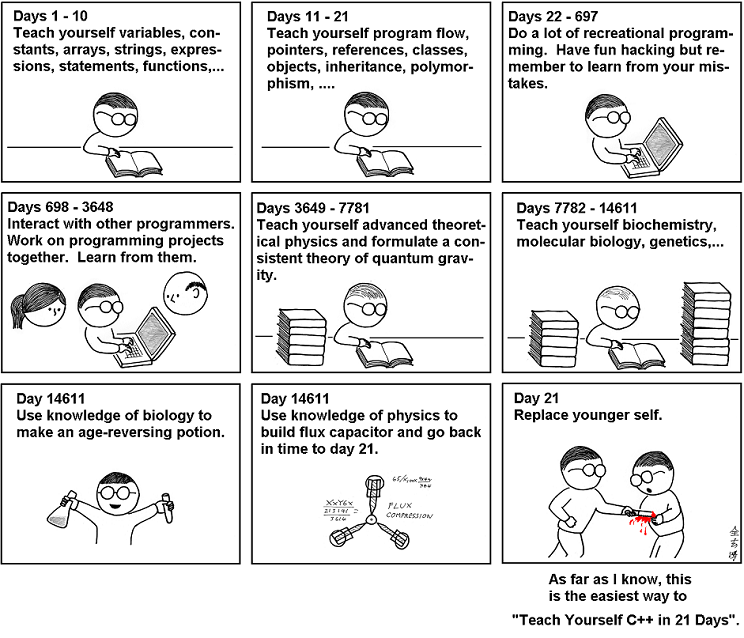
\includegraphics[width=\linewidth]{./gfx/agoose-249}
	\caption
		[Teach Yourself C++ in 21 days -- ein Praxisbericht.]
		{Teach Yourself C++ in 21 days -- ein Praxisbericht.\newline 
		 Quelle: \url{https://abstrusegoose.com/249}}
	\label{fig:gooseCPP}
\end{figure}


\section{Default Arguments und Function Overloading}
In C++ ist es möglich, Funktionen, die Parameter erwarten, Standardwerte vorzugeben. Beim Aufruf kann man dann diesen Parameter auslassen. Im Prototypen der Funktion wird dazu einfach hinter der Deklaration des Parameters ein \texttt{= Wert} angefügt. In der Kopfzeile der eigentlichen Funktion wird dies dann nicht mehr wiederholt.

\begin{codebox}[Beispiel: Funktion mit Default-Parameter]
\begin{minted}[linenos]{c++}
#include <iostream>

void showANumber(int number = 42);

void showANumber(int number) {
  std::cout << number << std::endl;
}

int main() {
   showANumber();
   showANumber(666);
}
\end{minted}
\end{codebox}

\begin{cmdbox}[Ausgabebeispiel: Funktion mit Default-Parameter]
42\\
666
\end{cmdbox}

\emph{Fakultative} (notwendige) und optionale Parameter (also solche, für die ein Standardwert vorgegeben wurde) können gemischt vorkommen; die optionalen Parameter müssen allerdings am Ende der Deklaration stehen.

Daneben ist es möglich, mehrere Funktionen mit demselben Bezeichner anzulegen, solange sich diese in der Signatur unterscheiden. Beispielsweise kann sich der Rückgabetyp unterscheiden oder die Zahl und Art der Parameter verschieden sein. Wir nennen dies \emph{Function Overloading}

Im Folgenden Beispiel benutzen wir Function Overloading, um mit einem Symbol Matrizen verschiedenen Datentyps (\mintinline{c++}{float} oder \mintinline{c++}{double}) anzulegen. Die Befehle \mintinline{c++}{new} und \mintinline{c++}{delete} sind für Sie noch neu, entsprechen in ihrer Funktion aber den Ihnen schon bekannten Befehlen \texttt{malloc} und \texttt{free}:

\begin{codebox}[Beispiel: Überladene Funktion]
\begin{minted}[linenos]{c++}
typedef struct {
  int     rows;
  int     cols;
  float*  data;
} matrixFloat;

typedef struct {
  int     rows;
  int     cols;
  double* data;
} matrixDouble;
\end{minted}
\end{codebox}

\begin{codebox}[]
\begin{minted}[linenos, firstnumber=last]{c++}
matrixFloat initMatrix(int rows, int cols) {
  matrixFloat reVal =  {-1, -1, nullptr};
  
  if (rows < 1 || cols < 1) {
    std::cout << "Unzulässige Matrix-Dimension" << std::endl;
    return reVal;
  }
  
  float * data = new float[rows * cols];
  if (!data) {
    std::cout << "Fehler beim Allozieren" << std::endl;
    return reVal;
  }
  
  reVal.rows = rows;
  reVal.cols = cols;
  reVal.data = data;
  
  return reVal;
}

matrixDouble initMatrix(int rows, int cols) {
  matrixDouble reVal =  {-1, -1, nullptr};
  
  if (rows < 1 || cols < 1) {
    std::cout << "Unzulässige Matrix-Dimension" << std::endl;
    return reVal;
  }
  
  double * data = new double[rows * cols];
  if (!data) {
    std::cout << "Fehler beim Allozieren" << std::endl;
    return reVal;
  }
  
  reVal.rows = rows;
  reVal.cols = cols;
  reVal.data = data;
  
  return reVal;
}

int main() {
   matrixFloat  mf = initMatrix(3, 3);
   matrixDouble md = initMatrix(3, 3);
   
   delete mf.data;
   delete md.data;
}
\end{minted}
\end{codebox}


\section{Templates}
Im obigen Beispiel gewinnen wir als ProgrammierInnen zwar in der \texttt{main} Klarheit des Codes, weil wir das Symbol \texttt{initMatrix} benutzen können, ohne uns weiter Gedanken über den Datentyp der erstellten Matrix machen zu müssen. Jedoch zwingt uns diese Struktur, Code doppelt zu schreiben: Bis auf die Allozierung von Speicher sind die Codes für die \mintinline{c++}{float}- und 
\mintinline{c++}{double}-Variante quasi gleich. Die ist schlecht, da es in der Weiterentwicklung unseres Codes leicht ist zu vergessen, Änderungen in einer Funktion auf ihr Pendant zu übertragen.

C++ erlaubt es daher, Funktionen für einen allgemeinen Datentypen zu schreiben. Der tatsächliche Datentyp wird erst im Aufruf eingesetzt. Wir nennen diese Technik \emph{Templates}. Über das Schlüsselwort \mintinline{c++}{template} wird ein Symbol definiert, das im folgenden Scope gültig ist und einen Typ beschreibt. Aufrufe einer Funktion mit einem Template-Typ \enquote{erzeugen} dann erst den tatsächlichen Code. Ähnlich wie bei Präprozessoren wird also Code erst umgeschrieben, bevor dieser kompiliert wird. Durch intellegentere Mechaniken tauchen aber weit weniger unerwartete Effekte auf.

Das obige Beispiel mit Matrizen lässt sich mit Templates so umschreiben:
\begin{codebox}[Beispiel: Überladene Funktion]
\begin{minted}[linenos]{c++}
template <typename T>
typedef struct {
  int  rows;
  int  cols;
  T *  data;
} matrix_t;

template <typename T>
matrix_t initMatrix(int rows, int cols) {
  matrix_t reVal =  {-1, -1, nullptr};
  
  if (rows < 1 || cols < 1) {
    std::cout << "Unzulässige Matrix-Dimension" << std::endl;
    return reVal;
  }
  
  T * data = new T[rows * cols];
  if (!data) {
    std::cout << "Fehler beim Allozieren" << std::endl;
    return reVal;
  }
  
  reVal.rows = rows;
  reVal.cols = cols;
  reVal.data = data;
  
  return reVal;
}
\end{minted}
\end{codebox}

\begin{codebox}[]
\begin{minted}[linenos, firstnumber=last]{c++}
int main() {
   matrix_t<float>  mf = initMatrix<float> (3, 3);
   matrix_t<double> md = initMatrix<double>(3, 3);
   
   delete mf.data;
   delete md.data;
}
\end{minted}
\end{codebox}

In den Zeilen 1 bis 6 definieren wir also eine Struktur, die Matrizen vom Typ \texttt{T} speichert. An dieser Stelle steht noch nicht fest, für welchen Datentyp \texttt{T} tatsächlich steht.

Die folgende Funktion \texttt{initMatrix} bereitet nun eine solche Matrix vor. Auch hier wird nur auf einen \emph{generischen} Datentyp \texttt{T} Bezug genommen; die Einsetzung für einen real existerenden Datentyp geschieht erst später.

In Zeile 30 dann wird eine Variable \texttt{mf} vom Typ \mintinline{c++}{matrix_T<float>} angelegt. Die <spitzen Klammern> sind der \emph{Template-Parameter}, also der \enquote{Wert}, der für \texttt{T} eingesetzt werden soll. An dieser Stelle wird also aus der Vorlage in den Zeilen 1 bis 6 ein \mintinline{c++}{struct} generiert, in dem \texttt{T} durch \mintinline{c++}{float} ersetzt wird. In der folgenden Zeile 31 passiert dasselbe für den Datentyp \mintinline{c++}{double}. Mit einfacher Tipparbeit sind also zwei Datentypen entstanden, die sich ein gemeinsames Gerüst teilen.

Dasselbe passiert in den Zeilen 30 und 31 für die Funktion \texttt{initMatrix}: Durch den Template-Parameter wird eine Variante der Funktion für \mintinline{c++}{float}s und eine Variante für \mintinline{c++}{double}s erzeugt\footnote{Bei den Funktionsaufrufen kann der Template-Parameter sogar entfallen. Da der Wert einer entsprechenden Variable zugeordnet werden soll, ist eindeutig vorgegeben, für welchen Zieltyp das Template umgesetzt werden soll.}.


\section{Klassen und Objektorientierung}
In C++ folgt man der Philosophie, gedankliche Einheiten in \emph{Objekten} abzubilden, die bestimmten \emph{Klassen} angehören. Eine Klasse ist eine Gruppe von Variablen zusammen mit \emph{Methoden}, über die mit diesem Objekt gearbeitet werden kann. Eine Klasse ist also eine Erweiterung der Idee einer \mintinline{c++}{struct} um Methoden. Hinzu kommt auch eine Einschränkung der Sichtbarkeit von Elementen der Klasse, ähnlich wie bei Scopes. Dies soll das versehentliche Ändern von Werten verhindern, die Nebeneffekte mit sich bringen und deren Veränderung einen inkonsistenten Programmzustand bewirken würden.

Objekte können zum Beispiel die oben angesprochenen Matrizen sein, oder eine Figur in einem Jump'n'Run-Spiel. Ein Codeauszug aus einem solchen Spiel könnte lauten:

\begin{codebox}[Beispiel: Überladene Funktion]
\begin{minted}[linenos]{c++}
class character {
private:
  int posX;
  int posY;
  int health;
  
public:
  void moveLeft();
  void moveRight();
  void jump();
}
\end{minted}
\end{codebox}

\begin{codebox}[]
\begin{minted}[linenos, firstnumber=last]{c++}
// Definition der Funktionen moveLeft, etc.

int main () {
  // ... Code ...
  character x;
  
  if (keyboard == right) {x.moveRight();}
}
\end{minted}
\end{codebox}

Das Schlüsselwort \texttt{private:} sperrt den Zugriff auf alle nachfolgenden Elemente der Klasse, also hier auf die Felder \texttt{posX}, \texttt{posY} und \texttt{health}. Nur Methoden derselben Klasse -- hier also \texttt{moveLeft}, \texttt{moveRight} und \texttt{jump} dürfen diese lesen oder verändern. Das Schlüsselwort \texttt{public:} hebt diese Einschränkung wieder auf: Alle nachfolgenden Deklarationen sind von jeder Stelle aus \enquote{sichtbar}.

Auf eine ähnliche Art können \emph{Constructors} und \emph{Destructors} definiert werden, \ie Methoden, die automatisch aufgerufen werden, sobald ein Objekt vom Typ der Klasse erstellt wird, bzw. sobald die Lebensdauer dieses Objekts endet. Damit muss man sich also nur einmal beim Erstellen der Klasse Gedanken um das Speichermanagement machen, und kann weiter in der Anwendung darauf vertrauen, dass diese Aufgabe bereits gelöst ist.


\section{Überladene Operatoren}
In Kapitel \ref{chp:structs} hatten wir festgestellt, dass für \mintinline{c++}{struct}s nur die Wertzuweisung (\texttt{=}) definiert ist. Alle anderen Operationen mussten dort über explizite Funktionsaufrufe erledigt werden.

In C++ ist es möglich, das Verhalten von Operatoren selbst zu definieren und damit auch neue Datentypen abzudecken. Das Verhalten wird in einer Funktion mit einer speziellen Kopfzeile definiert. Der \enquote{Aufruf} der Funktion geschieht dann über das Operatorsymbol.

Die Addition zweier Vektoren ließe sich in C++ beispielsweise so realisieren:

\begin{codebox}[Beispiel: Überladene Operatoren]
\begin{minted}[linenos]{c++}
typedef struct {
  double x;
  double y;
} vector2d_t;

vector2d_t operator + (vector2d_t LHS, vector2d_t RHS) {
  vector2d_t reVal = {LHS.x + RHS.x, LHS.y + RHS.y};
  return reVal;
}

int main {
  vector2d_t a = {42, 666}, b = {-420, 3.14};
  vector2d_t c = a + b;

}
\end{minted}
\end{codebox}


\section{Strings in C++}
Die aufwändigen und wiederkehrenden Aufgaben, die beim Umgang mit Texten in C auftreten, sind in C++ gesammelt und in der Klasse \texttt{std::string} abgehandelt. Mit dieser sind weiterhin die von C bekannten Techniken möglich. 

Als \emph{Klasse} stehen für Strings diverse \emph{Methoden} zur Verfügung, die über die oben gezeigte Syntax \texttt{object.method()} aufgerufen werden. Zur Verfügung stehen unter anderem Methoden zur Bestimmung der Länge, zur Verkettung oder zum Finden von Zeichenketten im String.

\begin{codebox}[Beispiel: Die \texttt{string}-Klasse]
\begin{minted}[linenos]{c++}
#include <iostream>
#include <string>

int main () {
  std::string 
     firstHalf = "Ich bin aus", 
     lastHalf  = " der Hölle",
     total;
  
  std::cout << firstHalf + lastHalf << std::endl;
  std::cout << (firstHalf + lastHalf).length() << std::endl;
  
  total = firstHalf + lastHalf;
  total.replace( total.find("aus"), 4, "Frau");
  total.replace( total.find("der"), 3, "");
  total[ total.find("ö") ] = 'o';
  std::cout << total << std::endl;
  
  firstHalf.insert( firstHalf.find("a"), "r" );
  
  std::cout << firstHalf << std::endl;
}
\end{minted}
\end{codebox}

\begin{cmdbox}[Ausgabebeispiel: Die \texttt{string}-Klasse]
Ich bin aus der Hölle \\
22\\
Ich bin Frau Holle\\
Ich bin raus
\end{cmdbox}

Alle Aufgaben des Speicher-Managements werden von der internen Mechanik der Klasse \texttt{string} automatisch übernommen.

Siehe auch \url{https://en.cppreference.com/w/cpp/string/basic_string} für weitere Details zur Klasse.


\section{Die Container-Library}
Neben Strings sind in der STL auch andere Klassen vorgefertigt, die die Arbeit mit größeren Datenmengen erleichtern. Listen beliebigen Datentyps können mit Hilfe dieser Klassen bequem angelegt, vergrößert und verkleinert werden. Wie schon bei Strings geschieht die Speicherverwaltung automatisch. Für verschiedene Anwendungsfälle stehen verschiedene Klassen zur Verfügung. Sie unterscheiden sich im Wesentlichen darin, welche Aufgaben die Methoden optimiert wurden. Für die meisten Anwendungsfälle ist die Klasse \texttt{std::vector} gut geeignet.

\begin{codebox}[Beispiel: Die \texttt{vector}-Klasse]
\begin{minted}[linenos]{c++}
#include <iostream>
#include <algorithm>
#include <vector>

int main () {
  std::vector<int> list;
  
  // make a list of numbers
  for (int i=0; i<20; i++) {list.push_back((i - 3) * (i - 1) * (i - 6));}
  
  // output on screen
  for (int i=0; i<20; i++) {std::cout << list[i] << " ";}
  std::cout << std::endl;
  
  // sort in ascending order
  std::sort(list.begin(), list.end());
  
  // output on screen
  for (int i=0; i<20; i++) {std::cout << list[i] << " ";}
  std::cout << std::endl;
}
\end{minted}
\end{codebox}

\begin{cmdbox}[Ausgabebeispiel: Die \texttt{vector}-Klasse]
-18 0 4 0 -6 -8 0 24 70 144 252 400 594 840 1144 1512 1950 2464 3060 3744\\ 
-18 -8 -6 0 0 0 4 24 70 144 252 400 594 840 1144 1512 1950 2464 3060 3744
\end{cmdbox}

Ähnlich funktionieren die folgenden Klassen:
\begin{description}
\item [\mintinline{c++}{std::array}]
	Wird auf dem Stack angelegt und kann nicht mehr in der Größe verändert werden. Viele Operationen
	laufen mit dieser Klasse schneller.
	(\url{https://en.cppreference.com/w/cpp/container/array})
\item [\mintinline{c++}{std::list}]
	Intern als Linked List umgesetzt. Einfügen an den Anfang und entfernen vom Anfang der Liste ist
	besonders schnell, ebenso ist Sortieren effizient programmiert. Diese Optimierung geht auf Kosten
	der Lesezeit für Elemente in der Mitte der Liste
	(\url{https://en.cppreference.com/w/cpp/container/list})
\item [\mintinline{c++}{std::map}]
	Implementiert ein \enquote{dictionary}, also eine Zuordnung von Wertepaaren zueinander. Anstelle
	eines Index wird also beispielsweise ein Wort als Schlüssel verwendet.
	(\url{https://en.cppreference.com/w/cpp/container/map})
\end{description}

Die Mechaniken hinter diesen Klassen werden z.\,T. in der Vorlesung \emph{Algorithmen und Datenstrukturen} an der Universität Regensburg besprochen.

	\appendix
\begin{appendices}
\chapter{Begriffe}
\section*{A...}
\begin{description}
\item[Adresse] \enquote{Nummer des Bytes im Speicher}, ab dem eine Information zu finden ist.\newline
	Siehe Abschnitt \ref{sec:Pointer}
\item[Adress-Operator] Das Zeichen \texttt{\&}. Wird vor Variablen gestellt, um den Speicherort (\ie die 
	\emph{Adresse}) der Variable zu ermitteln.\newline
	Siehe Abschnitt \ref{sec:Pointer}
\item[Allozieren] Anfrage an das Betriebssystem, einen Speicherbereich für andere Programme zu sperren,
	also den Speicherbereich für eine bestimmte Aufgabe zu \emph{reservieren}. Üblicherweise mit den 
	Befehlen \texttt{malloc} oder \texttt{calloc} aus dem \emph{Header} \texttt{<stdlib.h>} umgesetzt.
	\newline
	Siehe Abschnitt \ref{sec:allocation}
\item[Alphanumerisch] Schriftzeichen, die für menschliche Worte (im Englischen) üblich sind, sowie
	Ziffern: A-Z, a-z, 0-9.
\item[Argument] Wert, der einer \emph{Funktion} in runden Klammern \texttt{()} \emph{übergeben} wird.
	Die Funkion kann nun mit diesem Wert arbeiten. Argumente können \emph{Konstanten}, \emph{Variablen}
	oder komplexe \emph{Ausdrücke} sein.\newline
	Beispiel: Die Funktion \texttt{sin} erwartet ein \emph{Argument} vom \texttt{Datentyp} 
	\mintinline{c}{double}. Damit können als Argumente \eg \texttt{0}, \texttt{x} oder 
	\texttt{3.14 * x + acos(0)} möglich.\newline
	Siehe Abschnitt \ref{sec:funcs}
\item[Array] Eine Liste von Werten, die im Speicher \enquote{hintereinander} abgelegt wird. Zugriff auf
	die Elemente des Arrays geschieht über einen \emph{Pointer} auf den Listenanfang und einen
	\emph{Index}.\newline
	Siehe Abschnitt \ref{sec:Arrays}
\item[Assembler] Eine Programmiersprache und auch der Name einer Art von Programmen.\newline
	Die Befehle der Sprache Assembler entsprechen dem (sehr kleinen) Befehlssatz eines Prozessors. Daher
	ist in dieser Sprache eine sehr hardwarenahe, kleinschrittige Denkweise notwendig.\newline
	\emph{Hochsprachen} erlauben größere Abstraktion und dadurch eine für Menschen natürlichere
	Denkweise. Oft werden Hochsprachen-Programme erst in die Sprache Assembler übersetzt und dann von
	einem Assembler-Programm in \emph{Maschinensprache} weiter übersetzt.\newline
	Siehe Abschnitt \ref{sec:assembly}
\item[Ausdruck] Eine Folge von \emph{Konstanten}, \emph{Variablen} und \emph{Funktionsaufrufen}, die
	durch \emph{Operatoren} so miteinander verknüpft sind, dass daraus ein Wert berechnet werden kann.
	\newline
	Beispiele (jeweils durch Semikolons getrennt): \texttt{x + 9}; \texttt{42}; 
	\texttt{-sqrt(5.3) * 7 - y}; \texttt{x > y}.\newline
	Siehe Abschnitt \ref{sec:expressions}
\item[Ausschlussset-Schreibweise] Teil eines \emph{Format-Strings} bei \texttt{scanf}, der bei der
	Eingabe von \emph{Strings} benutzt wird. Form \mintinline{c}{[^...]}, wobei \texttt{...} für die
	Zeichen steht, die \emph{nicht} beachtet werden sollen.\newline
	Siehe Abschnitt \ref{sec:strInput}
\item[Automatische Arrays] \emph{Arrays}, die vom Compiler verwaltet werden, \ie für die kein
	Speicher mit \texttt{malloc} \emph{alloziert} werden muss, und die nicht mit \texttt{free}
	freigegeben werden dürfen. Bei der \emph{Deklaration} wird in [eckige Klammern] die Arraygröße in
	Elementen angegeben (Ausnahme: \emph{Initializer-List}).\\
	Einmal angelegt kann die Größe von automatischen Arrays nicht mehr geändert werden. Siehe daher auch 
	\emph{Dynamische Arrays}, die zur \emph{Laufzeit} die Größe ändern können\\
	Siehe Abschnitt \ref{sec:Arrays}

\section*{B...}
\item[Bibliothek] Eine Sammlung von \emph{Routinen}, die für sich genommen kein alleinstehendes Programm
	ergeben, die aber Probleme lösen, welche in anderen Programmen (mehrfach) auftreten können.
	Üblicherweise stehen Bibliotheken als \emph{vorkompilierte} Datenobjekte zur Verfügung. Sie werden
	über einen \emph{Header} in den eigenen Code eingebunden. Beim \emph{kompilieren} muss gegen die
	Bibliothek \emph{gelinkt} werden.\newline
	Siehe Abschnitt \ref{sec:Compile} und Kapitel \ref{chp:modules}
\item[Binärformat] Darstellung von Werten in einem Format, das von Computern leicht und effizient
	verarbeitet werden kann, das für Menschen dagegen \idR nicht entzifferbar ist. Dateien in diesem
	Format werden mit \texttt{fwrite} geschrieben und mit \texttt{fread} gelesen. Alle Werte im Speicher
	werden im Binärformat gehalten.\newline
	Siehe Abschnitt \ref{sec:binAccess}
\item[Binärsystem] Zahlensystem, das lediglich aus den Ziffern \texttt{0} und \texttt{1} besteht und die
	Grundlage der Rechner-Elektronik bildet. \newline
	Siehe Abschnitt \ref{sec:BinaryNumbers}
\item[Bitweise Operatoren] \emph{Operatoren}, die nicht mit Zahlen als Einheit arbeiten, sondern die die
	einzelnen Bits der Zahlen getrennt voneinander verarbeiten. Die Bitweisen Operatoren werden
	mit den Zeichen \texttt{\textasciicircum}, \texttt{\&}, \texttt{|} und \texttt{\^} gesetzt und sind
	von den \emph{logischen Operatoren} abzugrenzen.\newline
	Siehe Abschnitt \ref{sec:BitwiseOperator}

\section*{C...}
\item[Compiler] Ein Programm, das die Übersetzung von (menschenlesbarer) Programmiersprache in
	\emph{Maschinensprache} übernimmt. Häufig wird dabei zunächst als Zwischenschritt in
	\emph{Assembler} \emph{transpiliert}.\newline
	Umgangssprachlich wird das \emph{Linken} auch als Teil des Kompilier-Vorgangs aufgefasst.\newline
	Siehe Abschnitt \ref{sec:Compile}.
	
\section*{D...}
\item[Dateimodi] Lese- oder Schreibzugriff.\\
	Siehe Abschnitt \ref{sec:fileAccess}
\item[Datentyp] Die Art der Information, auf die über eine \emph{Variable} oder einen \emph{Ausdruck} 
	zugegriffen werden kann, bzw. die einer \emph{Konstanten} zugeordnet ist. Ein Datentyp kann eine von
	mehreren Arten von \emph{Ganzzahlen}, \emph{Fließkommazahlen} oder \emph{Pointern} sein.\\
	Siehe Abschnitt \ref{sec:expressions} sowie die Tabellen \ref{tab:DatatypesStd} und
	\ref{tab:DatatypesExt}
\item[Definition] Eine Anweisung, die zwar die Bedeutung eines Symbols festlegt, aber keine
	\emph{Speicherstelle} reserviert oder ändert.\\
	Siehe \emph{Forward declaration}, \emph{Header}, \emph{Präprozessor}.
\item[Deklaration] Abschnitt im Code, bei dem einem \emph{Symbol} innerhalb seines Scopes eine
	ein \emph{Datentyp} und eine \emph{Speicherstelle} zugewiesen werden (letzteres geschieht dabei
	automatisch).\\
	Siehe Abschnitte \ref{sec:DeclareVars} und \ref{sec:funcs}
\item[Dereferenzierung] Anweisung an den Compiler, nicht mit einem \emph{Pointer} zu arbeiten, sondern
	mit dem Wert im Speicher, der durch den Pointer referenziert wird. Dies geschieht entweder über den
	Dereferenzierungsoperator (\texttt{*pointer}) oder über den Array-Index-Zugriff
	(\texttt{pointer[index]})\\
	Siehe Abschnitte \ref{sec:Pointer} und \ref{sec:Arrays}.
\item[Dualsystem] Synonym für \emph{Binärsystem}
\item[Dynamische Arrays] \emph{Arrays}, die vom/von der ProgrammiererIn verwaltet werden, \ie für die
	Speicher mit \texttt{malloc} \emph{alloziert} werden muss, und die nicht mit \texttt{free}
	freigegeben werden müssen. Bei der \emph{Deklaration} wird das Symbol \texttt{*} benutzt, um
	das zugeordnete Symbol als \emph{Pointer} zu markieren.\\
	\emph{Dynamische Arrays} können zur \emph{Laufzeit} die Größe ändern, sind aber aufwändiger zu
	verwalten als \emph{Automatische Arrays}\\
	Siehe Abschnitt \ref{sec:Arrays}

\section*{E...}
\item[Errorcode] Eine \emph{Ganzzahl} zwischen 0 und 255, die eine Information darüber enthält, welche
	Fehler bei der Ausführung eines Programms aufgetreten sind.\\
	Siehe Abschnitt \ref{sec:errorcodes}
\item[Escape-Char, Escape-Sequenz] Ein Zeichen, das angibt, dass das oder die folgenden Zeichen eines
	Textes nicht eins zu eins umgesetzt werden sollen, sondern durch andere, schwer einzugebende Zeichen
	ersetzt	werden sollen (\eg Zeilenumbruch). In C ist das Escape-Char der Backslash
	\texttt{\textbackslash}.\\
	Escape-Char und \emph{Escape-Sequenz} werden zusammen durch eine Entsprechung ersetzt.\\
	Siehe Tabelle \ref{tab:Escape}
\item[Expansion] Der Code, der vom \emph{Präprozessor} erzeugt wird, nachdem ein \emph{Macro} durch
	seinen Macrotext ersetzt wurde.\\
	Siehe Kapitel \ref{chp:Preprocessor}

\section*{F...}
\item[Fließkommazahl] Eine Information, die eine Zahl mit Nachkomma-Anteil beschreibt, also \eg
	\texttt{3.14} oder auch \texttt{42.0}.\\
	Siehe Abschnitt \ref{sec:valueAssignment}
\item[Format-String] Eine Zeichenkette, die mit \texttt{printf}, \texttt{scanf} und den damit
	verwandeten Funktionen (\texttt{sprintf}, \texttt{fprintf}, \ldots) verwendet wird.\\
	Ein Format-String enthält Steuer-zeichenketten, die über Datentyp und Format von Werten informieren. 
	Diese Zeichenketten beginnen in der Regel mit einem Prozentsymbol \% und können aus einem oder 
	mehreren weiteren Zeichen bestehen.\\
	Siehe Tabellen \ref{tab:FormatOutNum}, \ref{tab:FormatOutSpc} und \ref{tab:FormatIn}
\item[Forward Declaration] Eine \enquote{unvollständige \emph{Deklaration}}, die notwendig ist, um
	Zirkelbezüge aufzulösen. Diese Technik kann mit \emph{Funktionen} und \emph{\mintinline{c}{struct}}s
	angewandt werden.\\
	Siehe Abschnitt \ref{sec:forwardDeclaration} und \ref{sec:typedef}
\item[Function-Body] Die eigentlichen Anweisungen, wie sie bei \emph{Funktionsaufruf} ausgeführt werden,
	eingefasst von \{geschweiften Klammern\}.\\
	Siehe Abschnitt \ref{sec:funcs}
\item[Funktion, Function] Ein Codeabschnitt, der einen eigentständigen \emph{Scope} definiert und eine
	allgemeine Lösung für ein Problem bereitstellt. Funktionen haben einen Namen, einen
	\emph{Rückgabetyp} und eine \emph{Parameterliste} (\ie null bis meherere \emph{Argumente}).\\
	Siehe Abschnitt \ref{sec:funcs}
\item[Funktionsaufruf] Der Befehl, mit der Code-Ausführung in eine \emph{Funktion} zu springen.\\
	Siehe Abschnitt \ref{sec:funcs}
\item[Funktionssignatur] Die Gesamtheit der Informationen \emph{Rückgabetyp} plus \emph{Parameterliste},
	ohne den Funktionsnamen. Man kann die Signatur einer Funktion als ihren \emph{Datentyp} auffassen.\\
	Siehe Abschnitt \ref{sec:funcs}

\section*{G...}
\item[Ganzzahl] Eine Information, die eine Zahl ohne Nachkomma-Anteil beschreibt, also \eg
	\texttt{3} oder auch \texttt{-42}.\\
	Siehe Abschnitt \ref{sec:valueAssignment}

\section*{H...}
\item[Header] Eine Code-Datei, die lediglich \emph{Definitionen} enthält: \emph{Funktions-Signaturen}
	ohne \emph{Function-Body}, \mintinline{c}{struct}s, \mintinline{c}{enum}s und 
	\mintinline{c}{typedef}s sowie \emph{Präprozessor-Direktiven}.\\
	Siehe Abschnitt \ref{sec:funcs}, und Kapitel \ref{chp:structs}, sowie \ref{chp:Preprocessor}
\item[Heap] (Großer) Speicherbereich, der dynamisch verwaltet werden kann, \ie in dem \ua
	\emph{dynamische Arrays} angelegt werden.\\
	Siehe Abschnitt \ref{sec:HeapStack}
\item[Hexadezimalsystem] Zahlensystem, das aus 16 Ziffern besteht (0, 1, 2, 3, 4, 5, 6, 7, 8, 9, A, B,
	C, D, E, F). Im Programmier- und Elektronik-Umfeld erlaubt dies eine platzsparende und
	übersichtliche Darstellung mancher Zusammenhänge.\newline
	Siehe Abschnitt \ref{sec:NumSystems}
\item[Hochsprache] Sprachen, die (gemessen am Befehlssatz eines Prozessors) komplexere Aufgaben in
	einem gedanklichen Schritt erledigen lassen. C ist noch sehr systemnah, zählt aber bereits als
	Hochsprache. Das Gegenstück bildet \emph{Assembler} mit einer (beinahen) eins-zu-eins-Entsprechung
	von Befehlen der Sprache und erzeugtem \emph{Maschinencode}.\\
	Siehe Abschnitt \ref{sec:assembly}

\section*{I...}
\item[Index] Nummer eines Elements in einer Liste. Indices beginnen in C bei 0!\\
	Siehe Abschnitt \ref{sec:Arrays}
\item[Initializer-List] Eine durch Kommata getrennte Liste von Werten, eingefasst in \{geschweiften
	Klammern\}. Wird zur gleichzeitigen \emph{Deklaration} und Wertzuweisung bei \emph{automatischen
	Arrays} und \mintinline{c}{struct}s gebraucht.\\
	Siehe Abschnitt \ref{sec:arrayInit} und \ref{sec:structInit}
\item[Instanz] Eine Speicherstelle, der ein Datentyp zugeordnet ist. Dieser Datentyp kann ein
	\emph{primitiver Datentyp} sein oder ein \mintinline{c}{struct}. Die Instanz ist also eine
	\emph{Variable} oder ein \emph{Array}-Element.\\
	Siehe Kapitel \ref{chp:structs}
\item[Iteration, Iterationsschritt] Wiederholung von ähnlichen Vorgängen in direkter Folge, häufig bei
	Veränderung von nur einer Variablen. Synonym für  \emph{Schleifen}. Ein \emph{Iterationsschritt} ist
	ein einzelner Durchlauf des \emph{Schleifenkörpers}.\\
	Siehe Kapitel \ref{chp:loops}

\section*{K...}
\item[Kommandozeile] Text-basiertes User-Interface, in das Kommandos eingegeben werden können, die vom
	Betriebssystem direkt umgesetzt werden. Im Kurs benutzt zum Aufruf des \emph{Compilers} und zum 
	Starten unserer Programme.\\
	Siehe Abschnitt \ref{sec:Compile}
\item[Kommandozeilen-Option] Teil des Textes, der in die \emph{Kommandozeile} eingegeben wird. Diese
	Optionen werden durch Leerzeichen vom Programmnamen und voneinander abgegrenzt, und beeinflussen
	den Programmablauf.\\
	Siehe Abschnitt \ref{sec:cmdlineParams}
\item[Kompilieren] Der Vorgang, bei dem ein menschenlesbarer Programmcode in Maschinensprache übersetzt
	wird. Umgangssprachlich wird das \emph{Linken} als Teil des Kompilierens aufgefasst.\\
	Siehe \emph{Compiler}, \emph{Linker}
\item[Kompilierzeit] Der Zeitpunkt, zu dem ein Programmcode in Maschinensprache übersetzt wird. Hier
	stehen noch nicht alle Informationen zur Verfügung, die zur \emph{Laufzeit} gegeben sind, \eg
	Usereingaben und damit Speicherbedarf. Dies macht dynamische Programmierung notwendig, also etwa
	\emph{dynamische Arrays}.\\
	Siehe Abschnitt \ref{sec:Arrays}
\item[Konstante] Ein Wert im Programm, der -- auch versehentlich -- nicht mehr geändert werden kann,
	sobald das Programm \emph{kompiliert} wurde. Beispiele: \mintinline{c}{3}, \mintinline{c}{"Dune"}
	
\section*{L...}
\item[Laufzeit] Der Zeitpunkt, an dem ein Programm ausgeführt wird. Hier stehen alle Informationen zur
	Verfügung (Usereingaben, Speicherbedarf, ...), aber es können keine strukturellen Änderungen am Code
	mehr durchgeführt werden, da das Programm bereits \emph{kompiliert} ist.\\
	Siehe Abschnitt \ref{sec:Arrays}
\item[Laufzeitverhalten] Die Beziehung von Zeitbedarf zu Datenmenge, die ein Algorithmus verarbeitet.
\item[Library] Englisch für \emph{Bibliothek}
\item[Linker] Ein Programm, das mehrere Dateien mit Code in \emph{Maschinensprache} zu einer einzigen,
	ausführbaren Datei zusammen fügt.
\item[Logische Operatoren] Operatoren, die mit \emph{Wahrheitswerten} operieren. In C existieren die
	logischen Operatoren \texttt{\&\&}, \texttt{||} und \texttt{!}.\\
	Siehe Abschnitt \ref{sec:OperatorsLogical}

\section*{M...}
\item[Macro, Makro] Textblöcke, die vom \emph{Präprozessor} durch anderen Text (Code) ersetzt werden.\\
	Siehe \emph{Expansion}, Kapitel \ref{chp:Preprocessor}
\item[Maschinensprache] Folge von Zahlenwerten, die Anweisungen für den Prozessor enthalten, und die
	vom Menschen nicht mehr (mit vertretbarem Aufwand) verstanden werden können. Wird beim
	\emph{kompilieren} erzeugt.\\
	Siehe Abschnitt \ref{sec:Compile}.
\item[Memory Leakage] Fehler in der Programmierung, bei der \emph{allozierter Speicher} nach
	Programmende nicht mehr freigegeben wird.\\
	Siehe Abchnitt \ref{sec:allocation}
\item[Menschenlesbares Format] Eine Darstellung von Information in für Menschen gedachte Schriftzeichen,
	Insbesondere durch die ASCII-Zeichen 32 bis 127. Daten im Menschenlesbaren Format sind \idR weniger
	effizient von Computern erfassbar als solche im \emph{Binärformat}.
\item[Modul] Eine Code-Einheit, die üblicherweise in einer einzelnen Datei abgelegt wird, und zunächst
	zu einem eigenständigen Object-File umgesetzt wird. Code eines Moduls \enquote{lebt} in einem
	eigenen Scope.\\
	Siehe Kapitel \ref{chp:modules}
\item[Modulo-Operator] Berechnet den Rest einer Division. Ausgedrückt durch das Prozent-Symbol \%.\\
	Siehe Abschnitt \ref{sec:OperatorsArithmetic}

\section*{N...}
\item[NAN] \enquote{not a number}. Ein Bitmuster, das bei \emph{Fließkommazahlen} als
	\enquote{Fehlerwert} gedeutet wird. Rechnungen, an denen eine NAN Anteil hat, haben zum Ergebnis
	wiederum eine NAN.
\item[Null-Char] Der Wert \mintinline{c}{0}, als \mintinline{c}{char} im Speicher abgelegt. Dieser Wert
	markiert das Ende eines \emph{Strings}.\\
	Siehe Abschnitt \ref{sec:string}

\section*{O...}
\item[Object-File] Datei bestehend aus \emph{Maschinencode}, der aus einem einzigen \emph{Modul} 
	stammt.\\
	Siehe Abschnitt \ref{sec:Compile}
\item[Offset] Englisch: \enquote{Versatz}: Der Abstand von einem bestimmten Anfangspunkt. Meist der
	Abstand vom Beginn eines \emph{Arrays} zu einer Speicherstelle, gemessen in Bytes; je nach Kontext
	aber auch in der Größeneinheit der Array-Elemente.
\item[Oktalsystem] Zahlensystem, das aus 8 Ziffern besteht (0 \ldots). Im Programmier- und Elektronik-
	Umfeld früher weit verbreitet. Heute nur noch im Kontext von Festplatten-Hardware üblich und
	weitgehend durch das \emph{Hexadezimalsystem} abgelöst\\
	Siehe Abschnitt \ref{sec:NumSystems}
\item[Operator] Eine Rechenanweisung. Wir unterscheiden unäre Operatoren, die nur einen einzigen Wert
	zur Berechnung des Ergebnisses brauchen (\eg. logisches und bitweises NOT, sowie das Vorzeichen
	Minus), binäre Operatoren (die zwei Zahlen brauchen, wie \eg \texttt{+}, \texttt{*}, \texttt{<{}<})
	\\
	Siehe Abschnitte \ref{sec:OperatorsLogical}, \ref{sec:OperatorsArithmetic}
\item[Overhead] Zusätzlicher Verwaltungsaufwand (für den Prozessor), der durch die Nutzung mancher
	Techniken notwendig wird und häufig nicht offensichtlich ist. Beispielsweise muss bei
	\emph{Funktionsaufrufen} der Codepunkt der Fortsetzung nach Funktionsende gespeichert werden,
	\emph{Parameter} kopiert werden und ein Programmsprung ausgeführt werden.

\section*{P...}
\item[Parameter, Parameterliste] Synonym für \emph{Argument}. Eine Parameterliste wird in runden
	Klammern () gesetzt und überhält die Werte, die an eine \emph{Funktion} übergeben werden.\\
	Siehe Abschnitt \ref{sec:funcs}
\item[Parität] Eigenschaft einer ganzen Zahl, gerade oder ungerade zu sein; man sagt also 1 hat ungerade
	Parätät, während 2 gerade Parität hat.
\item[Parsen] Sammelbegriff für das Deuten eines \emph{Strings} in einem bestimmten Kontext, also
	beispielsweise die Zerlegung in einzelne Worte oder die Verarbeitung eines \emph{Format-Strings}.
\item[Pointer] Typ von Variablen, die nicht eine Information selbst, sondern ihre \emph{Adresse} im
	Speicher enthalten.\\
	Siehe Abschnitt \ref{sec:Pointer}
\item[Präprozessor] Ein Programm, das (C-)Code \enquote{vorverarbeitet}, indem bestimmte Text-Elemente
	durch andere ersetzt werden.\\
	Siehe Kapitel \ref{chp:Preprocessor}
\item[Präprozessor-Direktive] Eine Anweisung an den \emph{Präprozessor}, die \eg festlegt, welche
	Ersetzungen vorgenommen werden sollen.
\item[Primitiver Datentyp] Datentypen, wie sie in der Sprache C ohne Zutun des/der ProgrammiererIn zur
	Verfügung stehen.\\
	Siehe Tabellen \ref{tab:DatatypesStd} und \ref{tab:DatatypesExt}
\item[Prototyp] Die erste Zeile einer \emph{Funktion}, in der \emph{Rückgabetyp}, Funktionsname und
	\emph{Parameterliste} zu finden sind.\\
	Siehe Abschnitt \ref{sec:funcs}
\item[Prozedur] Synonym für \emph{Funktion}.\\
	Siehe Abschnitt \ref{sec:funcs}

\section*{R...}
\item[Registerbreite] Die Zahl der Bits, die für eine \emph{Instanz} eines \emph{Datentyps} zur
	Verfügung stehen muss.
\item[Rekursion] Technik, bei der eine Funktion sich selbst aufruft.\\
	Siehe Kapitel \ref{chp:recursion}
\item[Rekursionstiefe] Die \enquote{Anzahl der Verschachtelungen} oder der Aufrufe der \emph{rekursiven}
	\emph{Funktion}\\
	Siehe Kapitel \ref{chp:recursion}
\item[Routine] Synonym für \emph{Funktion}.
\item[Rückgabetyp] Der \emph{Datentyp} des Wertes, der von einer \emph{Funktion} berechnet wird.\\
	Siehe Abschnitt \ref{sec:funcs}
\item[Rückgabewert] Der Wert, der von einer \emph{Funktion} berechnet wird.\\
	Siehe Abschnitt \ref{sec:funcs}

\section*{S...}
\item[Scope] Codeabschnitt, innerhalb dem die Bedeutung eines \emph{Symbols} definiert ist.\\
	Siehe Abschnitt \ref{sec:Scopes}
\item[Schleife] Code-Struktur, die mehrere ähnliche Anweisungen in direkter Folge wiederholt, und dabei
	häufig nur den Wert von einer oder wenigen Variablen verändert.\\
	Siehe Kapitel \ref{chp:loops}
\item[Schleifenkörper] Der Code in \{geschweiften Klammern\}, der durch die \emph{Schleife} wiederholt
	werden soll.\\
	Siehe Kapitel \ref{chp:loops}
\item[Segfault] Schwerer Fehler, der durch den falschen Umgang mit \emph{Pointern} entsteht. Beim
	unbeabsichtigten Zugriff auf eine Speicherstelle werden Werte überschrieben und führen zum
	Programmabsturz.
\item[Set-Schreibweise] Teil eines \emph{Format-Strings} bei \texttt{scanf}, der bei der
	Eingabe von \emph{Strings} benutzt wird. Form \mintinline{c}{[...]}, wobei \texttt{...} für die
	Zeichen steht, die für die Eingabe erlaubt sollen.\newline
	Siehe Abschnitt \ref{sec:strInput}
\item[Speicher Freigeben] Anweisung an das Betriebssystem, dass ein vorher \emph{allozierter}
	Speicherbereich nicht mehr benötigt wird und wieder für andere Programme zur Verfügung steht. Wird
	durch den Befehl \texttt{free} umgesetzt.\\
	Siehe Abschnitt \ref{sec:allocation}
\item[Speicher Reservieren] Anweisung an das Betriebssystem, dass Speicherplatz für eine bestimmte
	Aufgabe benötigt wird. Das Betriebssystem findet einen zusammenhängenden, genügend großen Block im
	Arbeitsspeicher und sperrt diesen für andere Prozesse. Wird durch die Befehle \texttt{malloc} und
	\texttt{calloc} umgesetzt.\\
	Siehe Abschnitt \ref{sec:allocation}
\item[Speicherstelle] Die Bytes im Arbeitsspeicher, an denen eine Information abgelegt ist.
\item[Signatur] Die Gesamtheit der Informationen \emph{Rückgabetyp} plus \emph{Parameterliste}, aber
	ohne den Namen der Funktion.\\
	Siehe Abschnitt \ref{sec:funcs}
\item[Stack] (Kleiner) Speicherbereich, der automatisch verwaltet wird, \ie in dem \ua
	\emph{automatische Arrays} sowie alle \enquote{einfachen Variablen} angelegt werden. Auf dem Stack
	wird außerdem die Rücksprungadresse bei \emph{Funktionsaufrufen} gespeichert.\\
	Siehe Abschnitt \ref{sec:HeapStack}
\item[Startadresse] Die \emph{Adresse} des ersten Werts eines \emph{Arrays}.\\
	Siehe Abschnitt \ref{sec:Arrays}
\item[String] Ein \emph{Array} aus \mintinline{c}{char}-Werten, das insbesondere Text enthält. Strings
	in C enden mit einem \emph{NULL-char}.\\
	Siehe Abschnitt \ref{sec:string}
\item[String-Literal] Eine \emph{String-Konstante}, also Text, eingefasst durch \texttt{''}doppelte
	Anführungszeichen\texttt{''}\\
	Siehe Abschnitt \ref{sec:string}
\item[Strong-Typed] Eigenschaft vieler Programmiersprachen, dass der \emph{Datentyp} einer
	\emph{Variablen} einmalig bei ihrer \emph{Deklaration} festgelegt wird und sich danach nicht mehr
	ändern kann.
\item[\mintinline{c}{struct}s] Benutzerdefinierte Datentypen, die aus mehreren 
	\emph{primitiven Datentypen} zusammengesetzt sind.\\
	Siehe Kapitel \ref{chp:structs}
\item[Symbol] Eine Folge von \emph{alphanumerischen} Zeichen sowie Unterstrichen (\texttt{\_}) die
	ein Konzept im Code bezeichnen. Ein solches Konzept kann \eg eine \emph{Variable}, ein
	Funktionsname, ein \mintinline{c}{struct}, \mintinline{c}{enum} oder eine 
	\emph{Präprozessor-Direktive} sein.
\item[Syntaxfehler] Eine Art von Programmierfehler, bei der der \emph{Compiler} die Arbeit abbricht. In
	der Regel handelt es sich um Tippfehler.

\section*{T...}
\item[Transpiler] Ein Programm, das Code von einer \emph{Hochsprache} in eine andere übersetzt.

\section*{U...}
\item[Übergeben von Werten] Teil eines \emph{Funktionsaufrufs}: Parameter von der aufrufenden Stelle
	werden an eine \emph{Speicherstelle} kopiert, mit der in der \emph{Funktion} gearbeitet werden kann
	\\
	Siehe Abschnitt \ref{sec:funcs}
	
\section*{V...}
\item[Variable] Ein Code\emph{symbol}, das auf eine \emph{Speicherstelle} verweist, deren Wert sich
	im Ablauf des Programms ändern kann.\\
	Siehe Abschnitt \ref{sec:expressions}

\section*{W...}
\item[Wahrheitswert] Die Information \enquote{wahr} oder \enquote{falsch} (\enquote{true} oder
	\enquote{false}). In C wird dies durch einen \emph{Ganzzahl}-Wert ausgedrückt, der entweder gleich
	null (false) oder ungleich null (true) ist.\\
	Siehe Abschnitt \ref{sec:truthvalues}

\section*{Z...}
\item[Zahlensystem] Die Gesamtheit an Symbolen, die als Ziffern verwendet werden. Gängig sind das
	Dezimalsystem und das \emph{Hexadezimalsystem}.
\end{description}



\chapter{Tabellen}
\section{Escape-Sequenzen}
\begin{table}[h!]
\newcolumntype{E}{>{\centering\ttfamily\arraybackslash}m{.3  \linewidth}}
\newcolumntype{F}{>{\centering         \arraybackslash}m{.65 \textwidth}}

\rowcolors{1}{white}{chameleonblue2}

\begin{tabularx}
	{\linewidth}
	{EF}
	\toprule[1.5pt]

	\normalfont	\bfseries Sequenz &
				\bfseries Funktion
	\tabcrlf
	
	\textbackslash a &
	\emph{alert} -- Ausgabe eines Tons über den Beeper, sofern vorhanden
	\\
	
	\textbackslash b &
	\emph{backspace} -- Textcursor um eine Spalte nach links verschieben
	\\
		
	\textbackslash f &
	\emph{form feed} -- Textcursor um eine Zeile nach unten verschieben
	\\
		
	\textbackslash n &
	\emph{newline} -- Textcursor an den Anfang der nächsten Zeile verschieben
	\\
		
	\textbackslash r &
	\emph{carriage return} -- Textcursor an den Anfang der aktuellen Zeile verschieben	
	\\
	
	\textbackslash t &
	\emph{horizontal tab} -- Textcursor auf die nächste Tabulator-Position nach rechts verschieben
	\\
	
	\textbackslash v &
	\emph{vertical tab} -- Textcursor auf die nächste \emph{vertikale} Tabulator-Position nach unten
						   verschieben
	\\
		
	\textbackslash \textbackslash  &
	\emph{backslash} -- das Zeichen \texttt{\textbackslash} selbst
	\\
		
	\textbackslash '' &
	\emph{double quote} -- das Zeichen \texttt{''} selbst
	\\
		
	\textbackslash x\texttt{hh} &
	\emph{ASCII character} -- das Zeichen mit dem ASCII-Code \texttt{0xhh} einfügen, wobei \texttt{hh}
							  ein Hexadezimalwert zwischen \texttt{00} und \texttt{FF} ist
	\\
		
	\textbackslash u\texttt{hhhh} &
	\emph{unicode character} -- das Unicode-Zeichen \texttt{0xhhhh} einfügen, wobei \texttt{hhhh} ein
								Hexadezimalwert zwischen \texttt{00} und \texttt{FFFF} ist
	\\
		
	\textbackslash U\texttt{hhhhhhhh} &
	\emph{unicode character} -- das Unicode-Zeichen \texttt{0xhhhhhhhh} einfügen, wobei
								\texttt{hhhhhhhh} ein Hexadezimalwert zwischen \texttt{00} und
								\texttt{FFFFFFFF} ist
	\\
	
	\%\% &
	\emph{percentage} -- das Prozentzeichen. Achtung: Hier werden tatsächlich zwei \% hintereinander
						 gesetzt, nicht der Backslash \textbackslash.
	\\
	
	\bottomrule[1.5pt]
\end{tabularx}
\caption{Escape-Sequenzen nach ISO/IEC 9899:TC3}
\label{tab:Escape}
\end{table}
Siehe Seite 19 auf \url{http://www.open-std.org/jtc1/sc22/wg14/www/docs/n1256.pdf}


\FloatBarrier
\section{Formatierte Textausgabe}
Die Format-Codes in Tabellen \ref{tab:FormatOutNum} und \ref{tab:FormatOutSpc} funktionieren sowohl mit \texttt{printf}, \texttt{sprintf}, \texttt{snprintf}, als auch mit \texttt{fprintf}.

Siehe auch \url{http://en.cppreference.com/w/c/io/fprintf}

\newcommand*{\tabsec}{\\ \cline{2-4}}
\newcommand*{\SLASH}{\char`\\}

\begin{table}[h!]
\newcolumntype{T}{>{\centering\ttfamily\arraybackslash}m{.15 \linewidth}}
\newcolumntype{S}{>{\centering\ttfamily\arraybackslash}m{.10 \textwidth}}
\newcolumntype{E}{>{\centering\ttfamily\arraybackslash}m{.35 \linewidth}}
\newcolumntype{C}{>{\centering         \arraybackslash}m{.29 \linewidth}}

\begin{tabularx}
	{\linewidth}
	{|T|S|E|C|}
	\toprule[1.5pt]

	\normalfont \bfseries Datentyp &
		\normalfont \bfseries format string &
		\normalfont \bfseries Beispiele &
		\normalfont \bfseries Anmerkung
\tabcrlf
	
\multirow{7}{*}{
	\makecell{
		\texttt{float} \\
		\normalfont oder \\
		\texttt{double}
	}
} & 
	\makecell{
		\%f \\
		\%lf 
	} & 
	\makecell{
		0.700000 \\
		1234567890123456768.000000
	} &
	Dezimalpunkt 
\tabsec
	
	& \%e &
	\makecell{
		7.0000000e-1 \\
		1.234568e+18 
	} &
	Exponentialschreibweise mit \enquote{e}
\tabsec

	& \%E &
	\makecell{
		7.0000000e-1 \\
		1.234568E+18 
	} &
	Exponentialschreibweise mit \enquote{E}
\tabsec

	& \%g &
	\makecell{
		0.7 \\
		1.234568e+18 
	} &
	Dezimal oder E-Schreibweise mit \enquote{e}
\tabsec

	& \%G &
	\makecell{
		0.7 \\
		1.234568E+18 
	} &
	Dezimal oder E-Schreibweise mit \enquote{E}
\tabsec

	& \%a &
	\makecell{
		0x1.6666666666666p-1  \\
		0x1.12210f47de981p+60 
	} &
	Hexadezimal mit Kleinbuchstaben
\tabsec

	& \%A &
	\makecell{
		0X1.6666666666666P-1  \\
		0X1.12210F47DE981P+60
	} &
	Hexadezimal mit Großbuchstaben
\tabcrlf

long double &
	\%Lf  &
	\normalfont wie bei \texttt{float} und \texttt{double} &
	Variationen (\texttt{\%Le}, ...) analog zu \texttt{float} und \texttt{double}
\tabcrlf

\multirow{2}{*}{char} & 
	\%c &
	A &
	als ASCII-Zeichen, Werte von 0 bis 255
\tabsec
	
	& \%hhi &
	65 &
	als Dezimalzahl, Werte von 0 bis 255
\tabcrlf

\multirow{6}{*}{\texttt{int}} &
	\makecell{
		\%d \\
		\%i
	} &
	\makecell{
		-1 \\
		2147483647
	} &
	Dezimal
\tabsec

	& \%u &
	\makecell{
		4294967295 \\
		2147483647
	} &
	Dezimal, ohne Vorzeichen 
\tabsec

	& \%o &
	\makecell{
		37777777777 \\
		17777777777
	} &
	Oktal, ohne Vorzeichen
\tabsec

	& \%x &
	\makecell{
		ffffffff \\
		7fffffff 
	} &
	Hexadezimal, ohne Vorzeichen, Kleinbuchstaben
\tabsec

	& \%X &
	\makecell{
		FFFFFFFF \\
		7FFFFFFF 
	} &
	Hexadezimal, ohne Vorzeichen, Grpßbuchstaben
\tabcrlf

long long int &
	\%lli, \%llx, ... &
	\makecell{
		-1 \\
		9223372036854775807
	} &
	alle Formen wie bei \texttt{int}, jeweils mit Präfix \texttt{ll}
\tabcrlf

short int &
	\%hi &
	\makecell{
		-1 \\
		32767 
	} &
	Variationen analog zu int \\

\bottomrule[1.5pt]
\end{tabularx}

\caption{Codes für formatierte Textausgabe (Zahlen)} \label{tab:FormatOutNum}
\end{table}

\begin{table}[h!]
\newcolumntype{T}{>{\centering\ttfamily\arraybackslash}m{.16 \linewidth}}
\newcolumntype{S}{>{\centering\ttfamily\arraybackslash}m{.10 \textwidth}}
\newcolumntype{E}{>{\centering\ttfamily\arraybackslash}m{.34 \linewidth}}
\newcolumntype{C}{>{\centering         \arraybackslash}m{.29 \linewidth}}

\begin{tabularx}
	{\linewidth}
	{|T|S|E|C|}
	\toprule[1.5pt]

	\normalfont \bfseries Datentyp &
		\normalfont \bfseries format string &
		\normalfont \bfseries Beispiele &
		\normalfont \bfseries Anmerkung
\tabcrlf

\multirow{5}{*}{\makecell{alle \\ Zahlen-Typen}} &
	\%+\textit{code} &
	\makecell{
		-1 \\
		+2147483647
	} &
	Ausgabe wie oben, immer mit Vorzeichen
\tabsec

	& \%N.M\textit{code} &
	\makecell{
		-0.70 \\
	 	1234567890123456768.00
	 } &
	Vorgabe: Mindestens Platz für \texttt{N} Zeichen; davon \texttt{M} für Nachkommastellen,
	rechtsbündig. Negative Zahlen für \texttt{N} und \texttt{M} machen die Ausgabe linksbündig.
\tabsec

	& \%0N.M\textit{code} &
	\makecell{
		-00.70 {\newline}
		1234567890123456768.00
	} &
	Vorgabe: wie oben, aber leere Stellen werden mit 0 aufgefüllt\tabcrlf
	
\makecell{
	{\ttfamily char*}, \\
	{\ttfamily char[]}, \\
	{\ttfamily unsigned~char*}
} &
	\%s &
	abcdefg &
	Als Zeichenkette; alle Zeichen von der adressierten Speicherstelle bis zum ersten 
	\texttt{NULL}-Zeichen.
\tabcrlf

\makecell{
	\textit{Datentyp} *\\
	\textsf{(Pointer)}
} & 
	\%p  &
	\makecell{
		 0x7fffc7a9dfb8 \\
		 (nil) 
	} & 
	Pointer auf beliebigen Datentyp, Ausgabe als Hexadezimalzahl.
	\texttt{NULL} wird als \texttt{(nil)} ausgegeben.
\\

\bottomrule[1.5pt]
\end{tabularx}
\caption{Codes für formatierte Textausgabe (Spacing und Strings)} \label{tab:FormatOutSpc}
\end{table}


\FloatBarrier
\section{Formatierte Texteingabe}
Die Format-Codes in Tabelle \ref{tab:FormatIn} funktionieren sowohl mit \texttt{scanf}, \texttt{sscanf}, \texttt{snscanf},  als auch mit \texttt{fscanf}.\\
Siehe auch \url{http://en.cppreference.com/w/c/io/fscanf}

\begin{table}[h!]
\newcolumntype{T}{>{\centering\ttfamily\arraybackslash}m{.20 \linewidth}}
\newcolumntype{S}{>{\centering\ttfamily\arraybackslash}m{.10 \linewidth}}
\newcolumntype{C}{>{\centering         \arraybackslash}m{.62\linewidth}}
\renewcommand*{\tabsec}{\\ \cline{1-2}}
\newcommand*  {\tabSec}{\\ \cline{2-3}}

\begin{tabularx}
	{\linewidth}
	{|T|S|C|}
	\toprule[1.5pt]
	
\normalfont \bfseries Pointer für Datentyp &
	\normalfont \bfseries format string &
	\normalfont \bfseries Anmerkung
	\tabcrlf
	
float &
	\%f &
	\multirow{3}{.75\linewidth}{
	Alle Schreibweisen (Dezimalpunkt, exponential, hexadezimal) werdenautomatisch erkannt) 
	}\tabsec

double &
	\%lf & \tabsec
	
long double &
	\%Lf & \tabcrlf
	
\multirow{2}{*}{int} 
	& \%i & 
	automatische Erkennung der Basis \tabSec
	
	& \%d & 
	dezimal \tabcrlf

\multirow{3}{*}{unsigned int} 
	& \%u & 
	vorzeichenlos, dezimal \tabSec
	
	& \%o & 
	vorzeichenlos, oktal \tabSec
	
	& \%x & 
	vorzeichenlos, hexadezimal \tabcrlf

\multirow{2}{*}{char} 
	& \%hhi 
	& Werte zwischen -128 und 127 \tabSec
	
	& \%c
	& ein Zeichen \tabcrlf

short int
	& \%hi, \%hu, ...
	& Variationen analog zu \texttt{int} und \texttt{unsigned int} \tabcrlf

long int 
	& \%li, \%lu, ...
	& Variationen analog zu \texttt{int} und \texttt{unsigned int} \tabcrlf
	

long long int 
	& \%lli, ...
	& Variationen analog zu \texttt{int} und \texttt{unsigned int} \tabcrlf
	
\multirow{7}{*}{
	\makecell{
		{\ttfamily char*}, \\
		{\ttfamily char[]}, \\
		{\ttfamily unsigned~char*}
	}
} 
	& \%s
	& Zeichenkette beliebiger Länge. Leerzeichen und Tabulatoren werden als Text-Ende interpretiert.
	\tabSec
	
	& \%Ns
	& Zeichenkette mit maximaler Länge N. Leerzeichen und Tabulatoren werden als Text-Ende interpretiert.
	\tabSec
	
	& \%[\textit{list}]s
	& Zeichenkette beliebiger Länge. Nur Zeichen, die in \textit{list} aufgeführt sind, werden akzeptiert. Der Ausdruck \textit{list} kann entweder eine Aneinanderreihung aller erlaubten Zeichen sein, oder ein Ausdruck der Art \emph{von-bis}. Alles hinter dem ersten Zeichen, das nicht in \textit{list} genannt wurde, wird ignoriert.\newline
	Beispiel 1: 
	\texttt{\%[0-9a-fA-F]} erlaubt Eingabe von Hexadezimalen Ganzzahlen\newline
	Beispiel 2:
	\texttt{\%[ \SLASH ta-z]} erlaubt Eingabe von Kleinbuchstaben, dem Tabulator und dem Leerzeichen.
	\\

	\bottomrule[1.5pt]
\end{tabularx}
\caption{Codes für formattierte Texteingabe} \label{tab:FormatIn}
\end{table}


\FloatBarrier
\section{UNIX/bash-Kommandos zum Formatieren}
Die Ausgabe der Zeichenketten (\eg mit \texttt{printf}) in den Tabellen \ref{tab:bashFormatCol} und \ref{tab:bashFormatSpc} wird von den auf \emph{unixoiden Systemen} (\eg Linux, Mac OS) üblichen Konsolen als Änderung des Ausgabeformats interpretiert. Die Details sind abhängig von der Implementierung der Konsole. Beschrieben hier ist die auf  verbreitete Konsole \emph{bash}. Die beschriebenen Farben stellen die Standard-Einstellungen dar und können bei jedem Anwender individuell angepasst werden.

\begin{table}[h!]
\newcolumntype{C}{>{\centering         \arraybackslash}m{.32\linewidth}}
\newcolumntype{F}{>{\centering\ttfamily\arraybackslash}m{.30\linewidth}}
\newcolumntype{B}{>{\centering\ttfamily\arraybackslash}m{.30\linewidth}}

\rowcolors{1}{white}{chameleonblue2}

\begin{tabularx}
	{\linewidth}
	{|C|F|B|}
	\toprule[1.5pt]

	\textbf{Farbe} &
		\normalfont \textbf{Schriftfarbe} &
		\normalfont \textbf{Hintergrund}
	\tabcrlf

	Schwarz  &
		\textbackslash x1b[30m &
		\textbackslash x1b[40m\\
	
	Rot  &
		\textbackslash x1b[31m &
		\textbackslash x1b[41m\\
	
	Grün  &
		\textbackslash x1b[32m &
		\textbackslash x1b[42m\\
	
	Braun  &
		\textbackslash x1b[33m &
		\textbackslash x1b[43m\\
	
	Blau  &
		\textbackslash x1b[34m &
		\textbackslash x1b[44m\\
	
	Magenta  &
		\textbackslash x1b[35m &
		\textbackslash x1b[45m\\
	
	Zyan  &
		\textbackslash x1b[36m &
		\textbackslash x1b[46m\\
	
	Grau  &
		\textbackslash x1b[37m &
		\textbackslash x1b[47m
	\tabcrlf

	Dunkelgrau  &
		\textbackslash x1b[90m &
		\textbackslash x1b[100m\\
	
	Hellrot  &
		\textbackslash x1b[91m &
		\textbackslash x1b[101m\\
	
	Hellgrün  &
		\textbackslash x1b[92m &
		\textbackslash x1b[102m\\
	
	Gelb  &
		\textbackslash x1b[93m &
		\textbackslash x1b[103m\\
	
	Hellblau  &
		\textbackslash x1b[94m &
		\textbackslash x1b[104m\\
	
	Pink  &
		\textbackslash x1b[95m &
		\textbackslash x1b[105m\\
	
	Hellzyan  &
		\textbackslash x1b[96m &
		\textbackslash x1b[106m\\
	
	Hellgrau  &
		\textbackslash x1b[97m &
		\textbackslash x1b[107m
	\tabcrlf
	
	(Standard-Farbe)  &
		\textbackslash x1b[39m &
		\textbackslash x1b[49m\\

	\bottomrule[1.5pt]
\end{tabularx}
\caption{UNIX/bash-Farbkommandos} \label{tab:bashFormatCol}
\end{table}

\begin{table}[h!]
\newcolumntype{C}{>{\centering         \arraybackslash}m{.32\linewidth}}
\newcolumntype{F}{>{\centering\ttfamily\arraybackslash}m{.30\linewidth}}
\newcolumntype{B}{>{\centering\ttfamily\arraybackslash}m{.30\linewidth}}

\rowcolors{1}{white}{chameleonblue2}

\begin{tabularx}
	{\linewidth}
	{|C|F|B|}
	\toprule[1.5pt]

	\textbf{Effekt} &
		\normalfont \textbf{Aktivieren} &
		\normalfont \textbf{Deaktivieren}
	\tabcrlf

	Normalen Text einstellen  &
		\textbackslash x1b[0m &
		\normalfont --\\
	
	Fettdruck  &
		\textbackslash x1b[1m &
		\textbackslash x1b[21m\\
	
	Kursivtext  &
		\textbackslash x1b[3m &
		\textbackslash x1b[23m\\
	
	Unterstreichung  &
		\textbackslash x1b[4m &
		\textbackslash x1b[24m\\
	
	Blinkend  &
		\textbackslash x1b[5m &
		\textbackslash x1b[25m\\
	
	Standardeinstellungen wiederherstellen &
		\textbackslash  033[m &
		\normalfont --\\
		
	\bottomrule[1.5pt]
\end{tabularx}
\caption{UNIX/bash-Formatkommandos} \label{tab:bashFormatSpc}
\end{table}


\FloatBarrier
\section{Operator-Hierarchie}
\begin{table}[h!]
	\rowcolors{1}{white}{chameleonblue2}
	\newcolumntype{P}{>{\centering \arraybackslash          } p{.2 \linewidth}}
	\newcolumntype{C}{>{\centering \arraybackslash \ttfamily} p{.2 \linewidth}}
	\newcolumntype{D}{>{\centering \arraybackslash          } p{.5\linewidth}}
\begin{tabularx}
		{\linewidth}
		{PCD}
		\toprule[1pt]

	\textbf{Priorität} & \normalfont\textbf{Operator} & \textbf{Beschreibung} \tabcrlf
	
	1  & \makecell{
			++, -{}-\\
			()\\
			{[]}\\
			., ->
		} & \makecell{
			Inkrement und Dekrement (Postfix) \\
			Funktionsaufruf\\
			Array-Indizierung\\
			Strukturzugriff
		} \\
	2  & \makecell{
			++, -{}-\\
			!, \textasciitilde \\
			(type) \\
			*\\
			\&\\
			sizeof
		} & \makecell{
			Inkrement und Dekrement (Prefix) \\
			Logisches und bitweises NOT \\
			Typecast\\
			Dereferenzierung\\
			Adresse finden\\
			Strukturgröße ermitteln
		} \\
	3  & *, /, \%                & Multiplikation, Division, Modulo\\
	4  & +, -                    & Addition, Subtraktion\\
	5  & <{}<, >{}>              & Bitshift nach links und rechts\\
	6  & \makecell{
			<, >\\
	 		<=, >=
	 	} &  \makecell{Vergleichsoperatoren kleiner/größer als \\
				 	   und kleiner gleich/größer gleich
		} \\
	7  & ==, != & Vergleichsoperatoren Gleichheit, Ungleichheit\\
	8  & \&                      & Bitweises AND\\
	9  & \textasciicircum        & Bitweises XOR\\
	10 & |                       & Bitweises OR\\
	11 & \&\& & Logisches AND\\
	12 & || & Logisches OR\\
	13 & ? : & Bedingte Auswertung (\emph{ternärer Operator})\\
	14 & = \\
	
	
	\bottomrule[1pt]	
\end{tabularx}
\caption{Präzedenz der Operatoren in C} \label{tab:OperatorPrecedence}
\end{table}

Siehe auch \url{https://en.cppreference.com/w/c/language/operator_precedence} für weitere Informationen.

\begin{plusbox}[C++: Erweiterte Liste von Operatoren]
Die Sprache C++ kennt einige weitere Operatoren, die hier nicht angesprochen werden können. Der Vollständigkeit halber sei dennoch auf den C++-spezifischen Artikel unter \url{https://en.cppreference.com/w/cpp/language/operator_precedence} verwiesen.
\end{plusbox}


\FloatBarrier
\section{Übersicht Datentypen} \label{sec:Datatypes}
Tabelle \ref{tab:DatatypesStd} beschreibt Datentypen, die immer zur Verfügung stehen. Grau gesetzte Werte sind plattformabhängig; hier ist jeweils die übliche Umsetzung auf modernen Rechnern angegeben.
\begin{table}[h!]
\rowcolors{1}{chameleonblue2}{white}
\newcolumntype{S}{>{\centering \arraybackslash} p{.19\linewidth}}
\newcolumntype{B}{>{\centering \arraybackslash} p{.54\linewidth}}

\begin{tabularx}
	{\linewidth}
	{SBS}
	\toprule[1pt]
	
	Datentyp      & Wertebereich                                & Speicherbedarf
\tabcrlf
	char          &               -128 \ldots              +127 & 1 Byte\\
	short int     &           -32\,768 \ldots          +32\,767 & 2 Byte\\
	int           &  \textcolor{grey}{-2\,147\,483\,648 \ldots +2\,147\,483\,647}
	                                                            & \textcolor{grey}{4 Byte}\\
	long int      & \textcolor{grey}{
                    -9\,223\,372\,036\,854\,775\,808 \ldots
	                +9\,223\,372\,036\,854\,775\,807}
	                                                            & \textcolor{grey}{8 Byte}\\
	long long int & -9\,223\,372\,036\,854\,775\,808 \ldots
	                +9\,223\,372\,036\,854\,775\,807
	                                                            & 8 Byte
\tabcrlf

	unsigned char          & 0 \ldots 255           				& 1 Byte\\
	unsigned short int     & 0 \ldots 65\,535         			& 2 Bytes\\
	unsigned int           & \textcolor{grey}{0 \ldots 4\,294\,967\,295}
																& \textcolor{grey}{4 Bytes}\\
	unsigned long int      & \textcolor{grey}{0 \ldots 1.8446744e+19}
																& \textcolor{grey}{8 Bytes}\\
	unsigned long long int & 0 \ldots 1.8446744e+19				& 8 Bytes
	
\tabcrlf

	float       & $\pm$3.4E+38, ca. 7 signifikante Ziffern    & 4 Byte\\	
	double      & $\pm$1.7E+308, ca. 16 signifikante Ziffern  & 8 Byte\\
	long double & \textcolor{grey}{sehr viel}                 & \textcolor{grey}{10 Byte}\\
	
\bottomrule[1pt]
\end{tabularx}
\caption{Standard-Datentypen der Sprache C} \label{tab:DatatypesStd}
\end{table}

Tabelle \ref{tab:DatatypesExt} beschreibt Datentypen, die zur Verfügung stehen, sobald der Header \texttt{stdint.h} eingebunden wird:
\begin{table}[h!]
\rowcolors{1}{white}{chameleonblue2}
\newcolumntype{S}{>{\centering \arraybackslash} p{.19\linewidth}}
\newcolumntype{B}{>{\centering \arraybackslash} p{.54\linewidth}}

\begin{tabularx}
	{\linewidth}
	{SBS}
	\toprule[1pt]
	
	Datentyp      & Wertebereich                                & Speicherbedarf
\tabcrlf
	int8\_t  &               -128 \ldots              +127 & 1 Byte\\
	int16\_t &           -32\,768 \ldots          +32\,767 & 2 Byte\\
	int32\_t &  -2\,147\,483\,648 \ldots +2\,147\,483\,647 & 4 Byte\\
	int64\_t & -9\,223\,372\,036\,854\,775\,808
	                                 \ldots
	                                        +9\,223\,372\,036\,854\,775\,807
	                                                          & 8 Byte
\tabcrlf

	uint8\_t   & 0 \ldots 255           & 1 Byte\\
	uint16\_t  & 0 \ldots 65\,535         & 2 Byte\\
	uint32\_t  & 0 \ldots 4\,294\,967\,295    & 4 Byte\\
	uint64\_t  & 0 \ldots 1.8446744e+19 & 8 Byte\\
	
\bottomrule[1pt]
\end{tabularx}
\caption{Standard-Datentypen der Sprache C} \label{tab:DatatypesExt}
\end{table}

Weitere Details können von der CPP-Referenz entnommen werden: 
\begin{itemize}
\item Standard-Typen: \url{https://en.cppreference.com/w/c/language/types}.
\item Erweiterte Ganzzahl-Typen: \url{https://en.cppreference.com/w/c/types/integer} (wie definiert in \texttt{stdint.h})
\end{itemize}

\begin{plusbox}[C++: Erweiterte Liste von Datentypen]
Die Sprache C++ wurde gegenüber C um einige Standard-Typen erweitert, die auf dem Artikel unter \url{https://en.cppreference.com/w/cpp/language/types} beschrieben werden.
\end{plusbox}

\section{Vordefinierte Präprozessor-Symbole}
Unter \url{https://gcc.gnu.org/onlinedocs/cpp/Predefined-Macros.html} finden Sie eine Liste von vordefinierten Macros. Für Betriebssystem-spezifische Macros, siehe \url{http://nadeausoftware.com/articles/2012/01/c_c_tip_how_use_compiler_predefined_macros_detect_operating_system}.

Hier seien einige der nützlichsten Macros aufgeführt\footnote{Ich beziehe mich hier auf den \texttt{gcc}; für andere Compiler haben die Macros ggf. andere Namen oder sind gar nicht definiert.}:

\begin{table}[h!]
\newcolumntype{E}{>{\centering\ttfamily\arraybackslash}m{.3  \linewidth}}
\newcolumntype{F}{>{\centering         \arraybackslash}m{.65 \textwidth}}

\rowcolors{1}{white}{chameleonblue2}

\begin{tabularx}
	{\linewidth}
	{EF}
	\toprule[1.5pt]

	\normalfont	\bfseries Macro &
				\bfseries Umsetzung
	\tabcrlf
	
	\_\_FILE\_\_ &
	String, der den Dateinamen der aktuell verarbeiteten Datei enthält
	\\
	
	\_\_LINE\_\_ &
	String, der die Nummer der Code-Zeile in der aktuell verarbeiteten Datei enthält
	\\
		
	\_\_func\_\_ &
	String, der die aktuell kompilierte Funktion enthält
	\\
		
	\_\_DATE\_\_ &
	String, der das Datum zur Kompilierzeit im Format \texttt{MMM DD YYYY} enthält.
	\\
		
	\_\_TIME\_\_ &
	String, der die Uhrzeit zur Kompilierzeit im Format \texttt{HH:MM:SS} enthält.
	\\
		
	\_\_VERSION\_\_ \textrm{und}  \_\_STDC\_VERSION\_\_ &
	String, der die Versionsnummer des Compilers enthält.
	\\
	
	\_\_unix\_\_ &
	Symbol ohne Inhalt, nur definiert, wenn für unixoide Systeme kompiliert wird
	\\
	
	\_\_linux\_\_ &
	Symbol ohne Inhalt, nur definiert, wenn für das Betriebssystem Linux kompiliert wird
	\\
	
	\_\_APPLE\_\_ &
	Symbol ohne Inhalt, nur definiert, wenn für das Betriebssysteme von Apple kompiliert wird
	\\
		
	\_\_WIN32\_\_  &
	Symbol ohne Inhalt, nur definiert, wenn für 32bit-Windows-Systeme kompiliert wird
	\\
		
	\_\_WIN64\_\_  &
	Symbol ohne Inhalt, nur definiert, wenn für 64bit-Windows-Systeme kompiliert wird
	\\
	
	\bottomrule[1.5pt]
\end{tabularx}
\caption{Vordefinierte Präprozessor-Symbole des \texttt{gcc}} \label{tab:predefinedMacros}
\end{table}

\chapter{Geschichte}
Der folgende Abschnitt ist eine freie Übersetzung von:\\
\url{https://www.techopedia.com/the-history-of-the-c-programming-language/2/32996}

\begin{wrapfigure}{r}{.4\linewidth}
	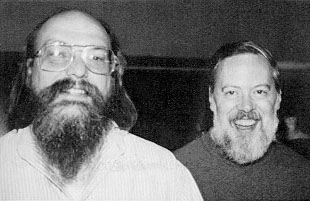
\includegraphics[width=\linewidth]{./gfx/KTDR}
	\caption%
		[Ken Thompson und Dennis Ritchie (1973) -- die Entwickler der Sprache C]
		{Ken Thompson und Dennis Ritchie (1973) -- die Entwickler der Sprache C\newline
		\url{https://en.wikipedia.org/wiki/Dennis_Ritchie}}
	\vspace{-20pt}
\end{wrapfigure}
Bis heute zählt die Sprache C zu einer der bedeutendsten Programmiersprachen. Von der Vielzahl an  Programmierpsprachen, die für verschiedenste Einsatzbereiche zur Verfügung stehen, ist ein Großteil von C beeinflusst. Ungeachtet der Existenz dieser Spezialisierungen bleibt C als Allzweck-Sprache von Bedeutung.

Es ist nicht bekannt, ob die Entwickler \emph{Dennis Ritchie} und \emph{Ken Thompson} bereits die Vision der großen Erfolge hatten, die die Sprache C einmal erreichen würde. Wie die meisten Innovationen sah auch C viele Veränderungen über die Zeit. Vermutlich der größte Erfolg ist die Tatsache, dass C bis in die jüngste Zeit hinein relevant blieb. Für die Entwickler ist es sicherlich sehr erfüllend zu sehen, dass C nicht als überholt oder als nur in Nischenanwendungen nützlich gilt. Stattdessen ist C als starke Allzweck-Sprache anerkannt.

Das Ursprüngliche Ziel der Entwickler war nicht die Entwicklung einer neuen Sprache. Tatsächlich war es erst das Zusammenspiel mehrerer Zufälle, die die Entwicklung der Sprache anstoßen. In den 1960ern arbeitete Dennis Ritchie bei Bell Labs (AT\&T) an einem Betriebssystem das von vielen Anwendern gleichzeitig benutzt werden konnte. Dieses Projekt \emph{MULTICS} (Multiplexed Information and Computer Services) sollte die gemeinsame Verwendung von Rechenressourcen erlauben. Von dem Projekt versprach man sich viele Verbesserungen -- aber bald stellte sich heraus, dass die Kosten für die Umsetzung die Vorteile überwiegen würden. Bell Labs zog sich graduell aus dem Projekt zurück.

Vor diesem Hintergrund schloss sich Ritchie dem Team von Ken Thompson und Brian Kernighan an. Thompson entwickelte in der Sprache Assembler ein Dateisystem für den DEC PDP-7 Supercomputer. Weitere Verbesserungen daran führten schließlich zur Konzeption des Betriebssystems UNIX, in dem einige der Ideen von MULTICS wieder auflebten. Tatsächlich weist schon der Originalname des neuen Projekts -- UNICS (Uniplexed Information and Computing Service) -- auf seine Verwandtschaft mit dem früheren Projekt hin.

UNIX wurde in Assembler geschrieben, was leicht für Computer umzusetzen ist, für Menschen aber eine herausfordernde Arbeitsumgebung darstellt. Um die Arbeit an UNIX zu erleichtern kamen die Sprachen Fortran und B zum Einsatz. Aus den Einschränkungen, die diese Sprachen brachten, erwuchs die Idee für die Sprache C.

Die Sprache B -- eine Weiterentwicklung der Sprache BCPL von Martin Richards -- stellte sich als nützliches Werkzeug in der Entwicklung von UNIX heraus. Jedoch mussten auch hier, wie auch in Assembler, Daten in Maschinensprache zur Verfügung gestellt werden. Datenstrukturen wurden in B ebenfalls nicht unterstützt.

Für die effiziente Fortsetzung der Arbeiten musste sich etwas ändern. Aus diesem Grunde machten sich Ritchie und seine Kollegen in den Jahren 1971 bis 73 daran, die Einschränkungen, die B ihnen auferlegte, abzuschalten. Es sollte nicht vergessen werden, dass die Sprache C im Geiste von B entwickelt wurde -- trotz oder gerade wegen dessen Beschränktheit. Viele Features und Konzepte wurden beibehalten, während neue Ideen -- darunter Datentypen und Strukturen -- hinzugefügt wurden. Der Name C weist direkt darauf hin, dass es sich hierbei um einen Nachfolger der Sprache B handelt. Anfangs wurde C im Hinblick auf die Arbeit an UNIX entwicklet. Um die Performance des Kernels und die Arbeit am Betriebssystem zu verbessern wurden viele UNIX-Komponenten neu in C umgeschrieben.

Ritchie und Kernighan dokumentierten ihr Werk in dem Buch \emph{The C Programming Language}. Obwohl Kernighan behauptete, keinen Einfluss auf das Design der Sprache C genommen zu haben, ist er doch der Autor vieler berühmter UNIX-Programme.

Bald begann C, in PCs für die Software-Entwicklung eingesetzt zu werden. Die erste (kleinere) Änderung am Sprachkonzept fand im Jahr 1983 statt, als das American National Standards Institute (ANSI) ein Kommittee zur Standardisierung der Sprache bildete. Einige Modifikationen wurden vorgenommen, die Code in der nun normierten Sprache kompatibler zu Vorgängerversionen machte. Im Jahre 1989 wurde der neue Standard verabschiedet und ist heute als ANSI C oder C89 bekannt. Die International Organization for Standardization (ISO) trug auch zur Standardisierung von C bei.

Im Laufe der Zeit hat sich C stark weiterentwickelt und Features wie Speichermanagement, Funktionen, Klassen und Bibliotheken in ihren Umfang aufgenommen und wird heute in einigen der größten und bekanntesten Projekte der Welt verwendet. Die Sprache beeinflusste die Entwicklung vieler anderer sprachen wie AMPL, AWK, csh, C++, C--, C\#, Objective-C, Bit C, D, Go, Java, JavaScript, Julia, Limbo, LPC, Perl, PHP, Pike, Processing, Python, Rust, Seed7, Vala und Verilog. 

Sind Sie ein Windows-User? Dann benutzen Sie ein Produkt, das vorwiegend in C geschrieben ist. Dasselbe gilt für MacOS, Linux, Android, iOS als auch für das Windows Phone -- kurz für alle modernen Betriebssysteme. Weiter findet C auch verbreitete Anwendung in Embedded Systems wie sie in Fahrzeugen, Smart TVs und den vielen Elementen des Internet of Things (IoT) verbaut sind.

Die vielfältigen Anwenungsfelder von C sind zu zahlreich, um sie hier aufzulisten. Einige jedoch seien als Beispiel genannt:
\begin{itemize}
\item Entwicklung von Compilern
\item Datenbanken 
\item Computer- und Handy-Spiele
\item Der UNIX-Kernel in seiner fortlaufenden Entwicklung
\item Auswertung Mathematischer Gleichungen
\item Design von Netzwerk-Geräten
\end{itemize}

Wie alle der großen Erfindungen entstand die Sprache C aus einer Notwendigkeit heraus. Die Probleme und Umstände der Zeit ihrer Entwicklung waren die Insporation für die Konzeption der Sprache. Anders als viele Sprachen, die heute als (fast) ausgestorben gelten, \enquote{gedeiht} C auch weiterhin. Einige Sprachen finden heute nur noch in Nischenbereichen Anwendung -- Fortran etwa kommt nur noch im Engineering-Bereich zum Einsatz, und COBOL hat kaum mehr Relevanz. C dagegen ist nicht nur weiterhin eine Sprache, die es zu kennen lohnt. Sie ist und bleibt Einfluss für die Weiterentwicklung bestehender und Konzeption neuer Sprachen. aufwändige Selbst Technologien wie das IoT, AI und Automations-Konzepte konnten sich nicht von der Sprache C lösen. Es bleibt zu erwarten, dass diese Sprache auch lange in die Zukunft ein Teil der Programmier-Welt bleiben wird.
\end{appendices}


	\listoffigures
\end{document}
